\documentclass[11pt, a4paper]{article}
\usepackage{epsfig}
\usepackage{graphicx}
\usepackage{amssymb, amsmath, amsthm, mathtools}
\usepackage[margin=2.5cm]{geometry}
\usepackage{siunitx}
\usepackage{booktabs}
\usepackage{caption}
\usepackage{pgfplots}
\usepackage{listings}
\usepackage{caption, subcaption}
% \usepackage{lmodern, microtype}
\usepackage{fontspec}
\usepackage[Latin,Greek]{ucharclasses}

\newfontfamily\substitutefont{FreeSerif}
\setTransitionsForGreek{\begingroup\substitutefont}{\endgroup}

\pgfplotsset{compat=newest}

\makeatletter
\def\fps@figure{hbtp}
\def\fps@table{hbtp}
\makeatother

\let\originalleft\left
\let\originalright\right
\renewcommand{\left}{\mathopen{}\mathclose\bgroup\originalleft}
\renewcommand{\right}{\aftergroup\egroup\originalright}

\DeclareMathOperator{\Normal}{Normal}
\DeclareMathOperator{\GammaD}{Gamma}
\DeclareMathOperator{\Bernoulli}{Bernoulli}
\DeclareMathOperator{\mean}{mean}
\DeclareMathOperator{\var}{var}
\DeclareMathOperator{\Id}{Id}

\lstset{
	breaklines=true,
	postbreak=\mbox{\textcolor{red}{$\hookrightarrow$}\space},
	}

\title{Assignment 6}
\author{Axel Forsman}

\begin{document}
\maketitle

\section{Introduction}
This laboration is concerned with stochastic processes,
which, simply said, are stochastic variables with a time parameter.
We first look at Brownian motions from physics.
Then we construct a new stochastic process based on the Brownian motion,
and try to approximate it using a cheaper recursive formula.
This leads to the question of how \emph{good} the approximation is.
Two measures of convergence are introduced for that purpose.

\section{Assignment 1}\label{sec:brownian_motion}
\subsection{Problem}
Plot a sample path of a Brownian motion for all $h_i = 2^{-i}, i = 1, \ldots, 10$
using the same noise throughout.
\subsection{Theory and implementation}
A \emph{stochastic process} $X \coloneqq (X(t), t \in \mathbb T \subset \mathbb R)$
is a collection of random variables indexed by $\mathbb T$.
Its \emph{sample path} is plot of $X(\omega, t)$ for a fixed $\omega \in \Omega$.
Moreover,
a \emph{Brownian motion} $W$ is a stochastic process given by
$$ W(t_n) \coloneqq W(t_{n-1}) + \eta^{(n)} $$
where $t_0, \ldots, t_N$ is a partition of $\mathbb T = [0, T]$,
$W(t_0) \coloneqq 0$ and $\eta \sim \mathcal N(0, h), \, h \coloneqq N^{-1}$.

To have the sample paths at the different resolutions use the same noise,
we generate $W_{h_{10}}$ and let
$$ \eta_{h_i}^{(n)} \coloneqq \eta_{h_{i+1}}^{(n)} + \eta_{h_{i+1}}^{(n+1)} \sim \mathcal N(0, 2h_{i+1})
	= \mathcal N(0, h_i) $$
That is, we can sum two finer increments to get the coarser increment.
\subsection{Results and discussion}
The sample path is shown in figure~\ref{fig:brownian_motion}.
We see that the paths become more and more jittery as we get to the finer resolutions,
as a result of the increased number of increments
each having an equal chance of being positive or negative.
Additionally, between every two adjacent endpoints of a path for a coarser resolution
there is one point of the immediately finer resolution,
that represents the further detail.

\begin{figure}
	\centering
	% This file was created by tikzplotlib v0.8.4.
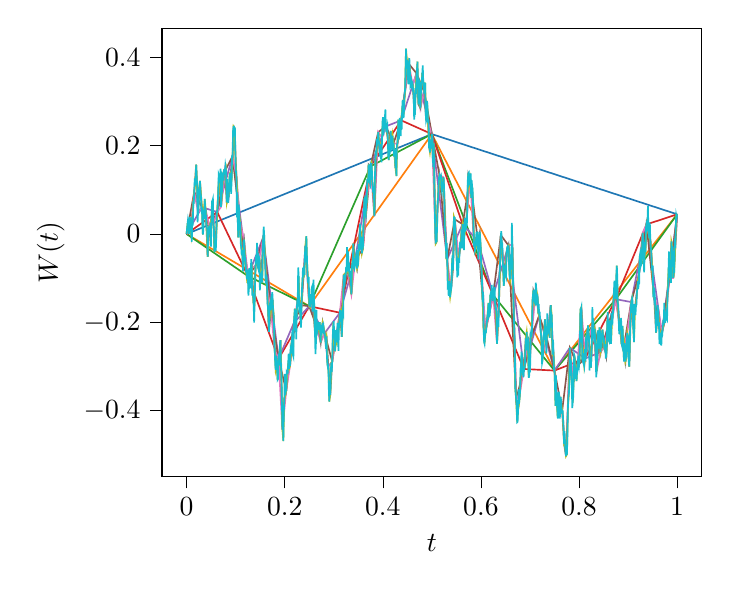
\begin{tikzpicture}

\definecolor{color0}{rgb}{0.12156862745098,0.466666666666667,0.705882352941177}
\definecolor{color1}{rgb}{1,0.498039215686275,0.0549019607843137}
\definecolor{color2}{rgb}{0.172549019607843,0.627450980392157,0.172549019607843}
\definecolor{color3}{rgb}{0.83921568627451,0.152941176470588,0.156862745098039}
\definecolor{color4}{rgb}{0.580392156862745,0.403921568627451,0.741176470588235}
\definecolor{color5}{rgb}{0.549019607843137,0.337254901960784,0.294117647058824}
\definecolor{color6}{rgb}{0.890196078431372,0.466666666666667,0.76078431372549}
\definecolor{color7}{rgb}{0.737254901960784,0.741176470588235,0.133333333333333}
\definecolor{color8}{rgb}{0.0901960784313725,0.745098039215686,0.811764705882353}

\begin{axis}[
tick align=outside,
tick pos=left,
x grid style={white!69.01960784313725!black},
xlabel={\(\displaystyle t\)},
xmin=-0.05, xmax=1.05,
xtick style={color=black},
y grid style={white!69.01960784313725!black},
ylabel={\(\displaystyle W(t)\)},
ymin=-0.549249892405815, ymax=0.465939421362371,
ytick style={color=black}
]
\addplot [semithick, color0]
table {%
0 0
0.5 0.226188299266531
1 0.0446367678077983
};
\addplot [semithick, color1]
table {%
0 0
0.25 -0.163477428547707
0.5 0.226188299266531
0.75 -0.309270056876883
1 0.0446367678077983
};
\addplot [semithick, color2]
table {%
0 0
0.125 -0.0952290895608764
0.25 -0.163477428547707
0.375 0.153316609039355
0.5 0.226188299266531
0.625 -0.138600696262659
0.75 -0.309270056876883
0.875 -0.147663601827953
1 0.0446367678077983
};
\addplot [semithick, color3]
table {%
0 0
0.0625 0.0498406463010942
0.125 -0.0952290895608764
0.1875 -0.282560705866867
0.25 -0.163477428547707
0.3125 -0.17821024233334
0.375 0.153316609039355
0.4375 0.257296812010063
0.5 0.226188299266531
0.5625 0.0220933241208356
0.625 -0.138600696262659
0.6875 -0.305677867892093
0.75 -0.309270056876883
0.8125 -0.282006474217183
0.875 -0.147663601827953
0.9375 0.0216241360304298
1 0.0446367678077983
};
\addplot [semithick, color4]
table {%
0 0
0.03125 0.0606067941849485
0.0625 0.0498406463010942
0.09375 0.176226423266858
0.125 -0.0952290895608764
0.15625 -0.00756850556480143
0.1875 -0.282560705866867
0.21875 -0.201295357378841
0.25 -0.163477428547707
0.28125 -0.224839619792612
0.3125 -0.17821024233334
0.34375 -0.0568086556033337
0.375 0.153316609039355
0.40625 0.243738622097754
0.4375 0.257296812010063
0.46875 0.363798493889044
0.5 0.226188299266531
0.53125 -0.057133985656343
0.5625 0.0220933241208356
0.59375 -0.0154172561142197
0.625 -0.138600696262659
0.65625 -0.0260238606155302
0.6875 -0.305677867892093
0.71875 -0.184772217913951
0.75 -0.309270056876883
0.78125 -0.25741473101758
0.8125 -0.282006474217183
0.84375 -0.267559392039037
0.875 -0.147663601827953
0.90625 -0.154107577114174
0.9375 0.0216241360304298
0.96875 -0.224514770945199
1 0.0446367678077983
};
\addplot [semithick, color5]
table {%
0 0
0.015625 0.0949638996083537
0.03125 0.0606067941849485
0.046875 0.0159279928293963
0.0625 0.0498406463010942
0.078125 0.142210765700092
0.09375 0.176226423266858
0.109375 0.0243038731543342
0.125 -0.0952290895608764
0.140625 -0.0722392995830708
0.15625 -0.00756850556480143
0.171875 -0.172837157714303
0.1875 -0.282560705866867
0.203125 -0.354712292590823
0.21875 -0.201295357378841
0.234375 -0.161391528650076
0.25 -0.163477428547707
0.265625 -0.211712732872344
0.28125 -0.224839619792612
0.296875 -0.288749282393864
0.3125 -0.17821024233334
0.328125 -0.0846418797739782
0.34375 -0.0568086556033337
0.359375 -0.0346857477057923
0.375 0.153316609039355
0.390625 0.230677285059979
0.40625 0.243738622097754
0.421875 0.205516965049848
0.4375 0.257296812010063
0.453125 0.385027346836459
0.46875 0.363798493889044
0.484375 0.322215098367622
0.5 0.226188299266531
0.515625 0.132708025359011
0.53125 -0.057133985656343
0.546875 0.0330655873051347
0.5625 0.0220933241208356
0.578125 0.124604646774031
0.59375 -0.0154172561142197
0.609375 -0.220308355338923
0.625 -0.138600696262659
0.640625 -0.00258580696152944
0.65625 -0.0260238606155302
0.671875 -0.374947461328615
0.6875 -0.305677867892093
0.703125 -0.231252048833452
0.71875 -0.184772217913951
0.734375 -0.236365538420743
0.75 -0.309270056876883
0.765625 -0.399674335779856
0.78125 -0.25741473101758
0.796875 -0.29738887769789
0.8125 -0.282006474217183
0.828125 -0.202550631355121
0.84375 -0.267559392039037
0.859375 -0.209972054624842
0.875 -0.147663601827953
0.890625 -0.260885746422818
0.90625 -0.154107577114174
0.921875 -0.0924616219561403
0.9375 0.0216241360304298
0.953125 -0.143691821340463
0.96875 -0.224514770945199
0.984375 -0.0999651399759821
1 0.0446367678077983
};
\addplot [semithick, color6]
table {%
0 0
0.0078125 0.00750542366524199
0.015625 0.0949638996083537
0.0234375 0.0496090905745811
0.03125 0.0606067941849485
0.0390625 0.0541602667863782
0.046875 0.0159279928293963
0.0546875 0.0239416108487721
0.0625 0.0498406463010942
0.0703125 0.0612710623590579
0.078125 0.142210765700092
0.0859375 0.0858049787449583
0.09375 0.176226423266858
0.1015625 0.13138563187588
0.109375 0.0243038731543342
0.1171875 -0.0130490910708574
0.125 -0.0952290895608764
0.1328125 -0.076479633100492
0.140625 -0.0722392995830708
0.1484375 -0.0549530718489272
0.15625 -0.00756850556480143
0.1640625 -0.121943250428684
0.171875 -0.172837157714303
0.1796875 -0.262449730663052
0.1875 -0.282560705866867
0.1953125 -0.443197811705809
0.203125 -0.354712292590823
0.2109375 -0.298385064604458
0.21875 -0.201295357378841
0.2265625 -0.148635686377056
0.234375 -0.161391528650076
0.2421875 -0.0262762615121445
0.25 -0.163477428547707
0.2578125 -0.165171417964965
0.265625 -0.211712732872344
0.2734375 -0.246117414425025
0.28125 -0.224839619792612
0.2890625 -0.300016114161143
0.296875 -0.288749282393864
0.3046875 -0.235778569975109
0.3125 -0.17821024233334
0.3203125 -0.0930329111546726
0.328125 -0.0846418797739782
0.3359375 -0.136670067080375
0.34375 -0.0568086556033337
0.3515625 -0.0363944804959497
0.359375 -0.0346857477057923
0.3671875 0.0717251504165042
0.375 0.153316609039355
0.3828125 0.0402912481427834
0.390625 0.230677285059979
0.3984375 0.217879790761237
0.40625 0.243738622097754
0.4140625 0.198054592321961
0.421875 0.205516965049848
0.4296875 0.20399571176038
0.4375 0.257296812010063
0.4453125 0.325544799378953
0.453125 0.385027346836459
0.4609375 0.337368540626418
0.46875 0.363798493889044
0.4765625 0.284649307961869
0.484375 0.322215098367622
0.4921875 0.252514872591599
0.5 0.226188299266531
0.5078125 -0.0219788646798917
0.515625 0.132708025359011
0.5234375 0.128747610749399
0.53125 -0.057133985656343
0.5390625 -0.126138951666179
0.546875 0.0330655873051347
0.5546875 -0.0542370608026445
0.5625 0.0220933241208356
0.5703125 0.0258775495809889
0.578125 0.124604646774031
0.5859375 -0.0244488360694108
0.59375 -0.0154172561142197
0.6015625 -0.0854772803455934
0.609375 -0.220308355338923
0.6171875 -0.177353233246973
0.625 -0.138600696262659
0.6328125 -0.248509039979496
0.640625 -0.00258580696152944
0.6484375 -0.0847920520557961
0.65625 -0.0260238606155302
0.6640625 -0.0238289675547193
0.671875 -0.374947461328615
0.6796875 -0.358766087750973
0.6875 -0.305677867892093
0.6953125 -0.246793541592899
0.703125 -0.231252048833452
0.7109375 -0.137858080427287
0.71875 -0.184772217913951
0.7265625 -0.271147567301344
0.734375 -0.236365538420743
0.7421875 -0.161369466976155
0.75 -0.309270056876883
0.7578125 -0.398981607955599
0.765625 -0.399674335779856
0.7734375 -0.503104923598171
0.78125 -0.25741473101758
0.7890625 -0.333566661517945
0.796875 -0.29738887769789
0.8046875 -0.166414263982712
0.8125 -0.282006474217183
0.8203125 -0.234418490290076
0.828125 -0.202550631355121
0.8359375 -0.310275733475615
0.84375 -0.267559392039037
0.8515625 -0.256696568419661
0.859375 -0.209972054624842
0.8671875 -0.196399527078721
0.875 -0.147663601827953
0.8828125 -0.20886395487942
0.890625 -0.260885746422818
0.8984375 -0.223910118636943
0.90625 -0.154107577114174
0.9140625 -0.168726988496781
0.921875 -0.0924616219561403
0.9296875 0.00237673140619113
0.9375 0.0216241360304298
0.9453125 -0.0137956920029042
0.953125 -0.143691821340463
0.9609375 -0.168445090129871
0.96875 -0.224514770945199
0.9765625 -0.189447521519726
0.984375 -0.0999651399759821
0.9921875 -0.0995064939869106
1 0.0446367678077983
};
\addplot [semithick, white!49.80392156862745!black]
table {%
0 0
0.00390625 0.0263962315661699
0.0078125 0.00750542366524199
0.01171875 0.0380399724328816
0.015625 0.0949638996083537
0.01953125 0.156842406289404
0.0234375 0.0496090905745811
0.02734375 0.120289925622556
0.03125 0.0606067941849485
0.03515625 0.0553094517344589
0.0390625 0.0541602667863782
0.04296875 -0.0514981832936526
0.046875 0.0159279928293963
0.05078125 0.0365201590246302
0.0546875 0.0239416108487721
0.05859375 -0.0224362032089515
0.0625 0.0498406463010942
0.06640625 0.131926776817921
0.0703125 0.0612710623590579
0.07421875 0.133371215725286
0.078125 0.142210765700092
0.08203125 0.0714055704422601
0.0859375 0.0858049787449583
0.08984375 0.13910629059502
0.09375 0.176226423266858
0.09765625 0.240697737319982
0.1015625 0.13138563187588
0.10546875 -0.00762576113177928
0.109375 0.0243038731543342
0.11328125 -0.036058800446301
0.1171875 -0.0130490910708574
0.12109375 -0.0828487239942866
0.125 -0.0952290895608764
0.12890625 -0.0940753058586704
0.1328125 -0.076479633100492
0.13671875 -0.158971472381434
0.140625 -0.0722392995830708
0.14453125 -0.05995998031238
0.1484375 -0.0549530718489272
0.15234375 -0.0907707810499254
0.15625 -0.00756850556480143
0.16015625 -0.0587028221711809
0.1640625 -0.121943250428684
0.16796875 -0.221334122378265
0.171875 -0.172837157714303
0.17578125 -0.157381234739689
0.1796875 -0.262449730663052
0.18359375 -0.29645239153525
0.1875 -0.282560705866867
0.19140625 -0.240652766705346
0.1953125 -0.443197811705809
0.19921875 -0.373261647113368
0.203125 -0.354712292590823
0.20703125 -0.296252315148166
0.2109375 -0.298385064604458
0.21484375 -0.2393744701935
0.21875 -0.201295357378841
0.22265625 -0.19963573102332
0.2265625 -0.148635686377056
0.23046875 -0.15526160597645
0.234375 -0.161391528650076
0.23828125 -0.0979507837257469
0.2421875 -0.0262762615121445
0.24609375 -0.0792059625392834
0.25 -0.163477428547707
0.25390625 -0.150331289069667
0.2578125 -0.165171417964965
0.26171875 -0.222872756276004
0.265625 -0.211712732872344
0.26953125 -0.217407873130758
0.2734375 -0.246117414425025
0.27734375 -0.200805442873365
0.28125 -0.224839619792612
0.28515625 -0.231913796558504
0.2890625 -0.300016114161143
0.29296875 -0.364518167816891
0.296875 -0.288749282393864
0.30078125 -0.218464022723796
0.3046875 -0.235778569975109
0.30859375 -0.229012590227173
0.3125 -0.17821024233334
0.31640625 -0.232986571174745
0.3203125 -0.0930329111546726
0.32421875 -0.0924936053327452
0.328125 -0.0846418797739782
0.33203125 -0.0967495599790372
0.3359375 -0.136670067080375
0.33984375 -0.0216939625756777
0.34375 -0.0568086556033337
0.34765625 -0.0782402646913226
0.3515625 -0.0363944804959497
0.35546875 -0.00614499587666713
0.359375 -0.0346857477057923
0.36328125 0.0816574471400288
0.3671875 0.0717251504165042
0.37109375 0.157716294016238
0.375 0.153316609039355
0.37890625 0.115346740660878
0.3828125 0.0402912481427834
0.38671875 0.176226359833509
0.390625 0.230677285059979
0.39453125 0.178092364608356
0.3984375 0.217879790761237
0.40234375 0.240526787947656
0.40625 0.243738622097754
0.41015625 0.216739306790557
0.4140625 0.198054592321961
0.41796875 0.198472268396748
0.421875 0.205516965049848
0.42578125 0.150001828456082
0.4296875 0.20399571176038
0.43359375 0.2257011351187
0.4375 0.257296812010063
0.44140625 0.295514270586683
0.4453125 0.325544799378953
0.44921875 0.393534823533129
0.453125 0.385027346836459
0.45703125 0.345190318817798
0.4609375 0.337368540626418
0.46484375 0.269977367105124
0.46875 0.363798493889044
0.47265625 0.29353388613458
0.4765625 0.284649307961869
0.48046875 0.364023825344129
0.484375 0.322215098367622
0.48828125 0.257868279073694
0.4921875 0.252514872591599
0.49609375 0.18463987104118
0.5 0.226188299266531
0.50390625 0.205221248349695
0.5078125 -0.0219788646798917
0.51171875 0.06870842022355
0.515625 0.132708025359011
0.51953125 0.101886100867533
0.5234375 0.128747610749399
0.52734375 0.00788460927000829
0.53125 -0.057133985656343
0.53515625 -0.125672890548181
0.5390625 -0.126138951666179
0.54296875 -0.0822779939939632
0.546875 0.0330655873051347
0.55078125 -0.0582517338477929
0.5546875 -0.0542370608026445
0.55859375 -0.028822665828881
0.5625 0.0220933241208356
0.56640625 0.0238165367931883
0.5703125 0.0258775495809889
0.57421875 0.136358955315751
0.578125 0.124604646774031
0.58203125 0.107778145952784
0.5859375 -0.0244488360694108
0.58984375 -0.0174323640707271
0.59375 -0.0154172561142197
0.59765625 0.00396721560635573
0.6015625 -0.0854772803455934
0.60546875 -0.215288326386932
0.609375 -0.220308355338923
0.61328125 -0.186602195083765
0.6171875 -0.177353233246973
0.62109375 -0.13724981850899
0.625 -0.138600696262659
0.62890625 -0.159260193265509
0.6328125 -0.248509039979496
0.63671875 -0.161522907806613
0.640625 -0.00258580696152944
0.64453125 -0.060802295929
0.6484375 -0.0847920520557961
0.65234375 -0.0425329917772428
0.65625 -0.0260238606155302
0.66015625 -0.102262032210925
0.6640625 -0.0238289675547193
0.66796875 -0.219944922929224
0.671875 -0.374947461328615
0.67578125 -0.397594486540326
0.6796875 -0.358766087750973
0.68359375 -0.275970135059472
0.6875 -0.305677867892093
0.69140625 -0.236656605824755
0.6953125 -0.246793541592899
0.69921875 -0.299978892047295
0.703125 -0.231252048833452
0.70703125 -0.126815741800246
0.7109375 -0.137858080427287
0.71484375 -0.13694585014441
0.71875 -0.184772217913951
0.72265625 -0.229978523995509
0.7265625 -0.271147567301344
0.73046875 -0.193515943991879
0.734375 -0.236365538420743
0.73828125 -0.220979256039149
0.7421875 -0.161369466976155
0.74609375 -0.272992527498911
0.75 -0.309270056876883
0.75390625 -0.371473420466688
0.7578125 -0.398981607955599
0.76171875 -0.404719139941017
0.765625 -0.399674335779856
0.76953125 -0.475628872552948
0.7734375 -0.503104923598171
0.77734375 -0.391719387590152
0.78125 -0.25741473101758
0.78515625 -0.333971207221557
0.7890625 -0.333566661517945
0.79296875 -0.305124893610988
0.796875 -0.29738887769789
0.80078125 -0.289785409585198
0.8046875 -0.166414263982712
0.80859375 -0.269700975899721
0.8125 -0.282006474217183
0.81640625 -0.226483545664001
0.8203125 -0.234418490290076
0.82421875 -0.302399406767347
0.828125 -0.202550631355121
0.83203125 -0.215419791367675
0.8359375 -0.310275733475615
0.83984375 -0.244703208428599
0.84375 -0.267559392039037
0.84765625 -0.216607028796237
0.8515625 -0.256696568419661
0.85546875 -0.277846718638333
0.859375 -0.209972054624842
0.86328125 -0.195657413405065
0.8671875 -0.196399527078721
0.87109375 -0.130776411481616
0.875 -0.147663601827953
0.87890625 -0.156656610991417
0.8828125 -0.20886395487942
0.88671875 -0.248801583743796
0.890625 -0.260885746422818
0.89453125 -0.289063460034515
0.8984375 -0.223910118636943
0.90234375 -0.300327242483637
0.90625 -0.154107577114174
0.91015625 -0.207021984596591
0.9140625 -0.168726988496781
0.91796875 -0.132022667917891
0.921875 -0.0924616219561403
0.92578125 -0.0523759759356481
0.9296875 0.00237673140619113
0.93359375 -0.0520886717469625
0.9375 0.0216241360304298
0.94140625 0.00866443189137601
0.9453125 -0.0137956920029042
0.94921875 -0.0819817196248202
0.953125 -0.143691821340463
0.95703125 -0.223360218369492
0.9609375 -0.168445090129871
0.96484375 -0.223145037349761
0.96875 -0.224514770945199
0.97265625 -0.206389570522446
0.9765625 -0.189447521519726
0.98046875 -0.132568269239262
0.984375 -0.0999651399759821
0.98828125 -0.0170142944554604
0.9921875 -0.0995064939869106
0.99609375 -0.0315024580347488
1 0.0446367678077983
};
\addplot [semithick, color7]
table {%
0 0
0.001953125 0.0232871603362519
0.00390625 0.0263962315661699
0.005859375 0.0150384479705233
0.0078125 0.00750542366524199
0.009765625 -0.00482878149200773
0.01171875 0.0380399724328816
0.013671875 0.0713351002779234
0.015625 0.0949638996083537
0.017578125 0.112171955968573
0.01953125 0.156842406289404
0.021484375 0.111113449722117
0.0234375 0.0496090905745811
0.025390625 0.0988853927096341
0.02734375 0.120289925622556
0.029296875 0.0864072463907575
0.03125 0.0606067941849485
0.033203125 -0.00127862530076411
0.03515625 0.0553094517344589
0.037109375 0.0792281516374222
0.0390625 0.0541602667863782
0.041015625 0.0158958550817062
0.04296875 -0.0514981832936526
0.044921875 0.00507037300003466
0.046875 0.0159279928293963
0.048828125 0.0256422492020869
0.05078125 0.0365201590246302
0.052734375 0.0752240615830723
0.0546875 0.0239416108487721
0.056640625 -0.0402462598581825
0.05859375 -0.0224362032089515
0.060546875 -0.00744409587095423
0.0625 0.0498406463010942
0.064453125 0.0952351264186752
0.06640625 0.131926776817921
0.068359375 0.116514939203743
0.0703125 0.0612710623590579
0.072265625 0.0971114947186668
0.07421875 0.133371215725286
0.076171875 0.143955387942964
0.078125 0.142210765700092
0.080078125 0.149156983957442
0.08203125 0.0714055704422601
0.083984375 0.0818905383416038
0.0859375 0.0858049787449583
0.087890625 0.137230505007555
0.08984375 0.13910629059502
0.091796875 0.118860152474113
0.09375 0.176226423266858
0.095703125 0.243889287053919
0.09765625 0.240697737319982
0.099609375 0.172111122613549
0.1015625 0.13138563187588
0.103515625 0.0942599239507356
0.10546875 -0.00762576113177928
0.107421875 0.0421341045097762
0.109375 0.0243038731543342
0.111328125 -0.0293777761217829
0.11328125 -0.036058800446301
0.115234375 -0.084384864845623
0.1171875 -0.0130490910708574
0.119140625 -0.053766325755176
0.12109375 -0.0828487239942866
0.123046875 -0.102687635533628
0.125 -0.0952290895608764
0.126953125 -0.125535477587916
0.12890625 -0.0940753058586704
0.130859375 -0.0816394392427401
0.1328125 -0.076479633100492
0.134765625 -0.133303148137123
0.13671875 -0.158971472381434
0.138671875 -0.160370684845608
0.140625 -0.0722392995830708
0.142578125 -0.0578801820558323
0.14453125 -0.05995998031238
0.146484375 -0.0796051238031616
0.1484375 -0.0549530718489272
0.150390625 -0.103278262440399
0.15234375 -0.0907707810499254
0.154296875 -0.110106722463679
0.15625 -0.00756850556480143
0.158203125 -0.00292746164833332
0.16015625 -0.0587028221711809
0.162109375 -0.11114266160513
0.1640625 -0.121943250428684
0.166015625 -0.168010024583614
0.16796875 -0.221334122378265
0.169921875 -0.157747685058733
0.171875 -0.172837157714303
0.173828125 -0.139920847305001
0.17578125 -0.157381234739689
0.177734375 -0.186742028494335
0.1796875 -0.262449730663052
0.181640625 -0.307367084756947
0.18359375 -0.29645239153525
0.185546875 -0.330191026500355
0.1875 -0.282560705866867
0.189453125 -0.297701195172807
0.19140625 -0.240652766705346
0.193359375 -0.313880392664538
0.1953125 -0.443197811705809
0.197265625 -0.46879303357154
0.19921875 -0.373261647113368
0.201171875 -0.365300445998884
0.203125 -0.354712292590823
0.205078125 -0.315756873521809
0.20703125 -0.296252315148166
0.208984375 -0.305474032260795
0.2109375 -0.298385064604458
0.212890625 -0.269529589939583
0.21484375 -0.2393744701935
0.216796875 -0.27415673782097
0.21875 -0.201295357378841
0.220703125 -0.168962073116153
0.22265625 -0.19963573102332
0.224609375 -0.176105373968778
0.2265625 -0.148635686377056
0.228515625 -0.0961853582436953
0.23046875 -0.15526160597645
0.232421875 -0.195043873979939
0.234375 -0.161391528650076
0.236328125 -0.101062675130361
0.23828125 -0.0979507837257469
0.240234375 -0.0926308982926995
0.2421875 -0.0262762615121445
0.244140625 -0.00487309381690309
0.24609375 -0.0792059625392834
0.248046875 -0.110570504652723
0.25 -0.163477428547707
0.251953125 -0.16604761546756
0.25390625 -0.150331289069667
0.255859375 -0.119632223767659
0.2578125 -0.165171417964965
0.259765625 -0.147099714632839
0.26171875 -0.222872756276004
0.263671875 -0.248525794209365
0.265625 -0.211712732872344
0.267578125 -0.211496772362654
0.26953125 -0.217407873130758
0.271484375 -0.199804232017033
0.2734375 -0.246117414425025
0.275390625 -0.217137260315202
0.27734375 -0.200805442873365
0.279296875 -0.210759360920784
0.28125 -0.224839619792612
0.283203125 -0.242454892262259
0.28515625 -0.231913796558504
0.287109375 -0.295808228133019
0.2890625 -0.300016114161143
0.291015625 -0.379710467614765
0.29296875 -0.364518167816891
0.294921875 -0.291654060860531
0.296875 -0.288749282393864
0.298828125 -0.211183902770684
0.30078125 -0.218464022723796
0.302734375 -0.265757661360059
0.3046875 -0.235778569975109
0.306640625 -0.245164877106894
0.30859375 -0.229012590227173
0.310546875 -0.212415697039078
0.3125 -0.17821024233334
0.314453125 -0.172496037054829
0.31640625 -0.232986571174745
0.318359375 -0.177517208196036
0.3203125 -0.0930329111546726
0.322265625 -0.0902273620289791
0.32421875 -0.0924936053327452
0.326171875 -0.0868182008700163
0.328125 -0.0846418797739782
0.330078125 -0.0758187937924795
0.33203125 -0.0967495599790372
0.333984375 -0.0997637978670162
0.3359375 -0.136670067080375
0.337890625 -0.0657166506725158
0.33984375 -0.0216939625756777
0.341796875 -0.0796629103969444
0.34375 -0.0568086556033337
0.345703125 -0.0491919728121229
0.34765625 -0.0782402646913226
0.349609375 -0.0713338444841452
0.3515625 -0.0363944804959497
0.353515625 0.0230000827880981
0.35546875 -0.00614499587666713
0.357421875 -0.0439205208328652
0.359375 -0.0346857477057923
0.361328125 0.0372041936776117
0.36328125 0.0816574471400288
0.365234375 0.0414711130364623
0.3671875 0.0717251504165042
0.369140625 0.116411496367838
0.37109375 0.157716294016238
0.373046875 0.118677514795719
0.375 0.153316609039355
0.376953125 0.160379096720897
0.37890625 0.115346740660878
0.380859375 0.0990937598416174
0.3828125 0.0402912481427834
0.384765625 0.168374177899138
0.38671875 0.176226359833509
0.388671875 0.205123184377808
0.390625 0.230677285059979
0.392578125 0.20723909488803
0.39453125 0.178092364608356
0.396484375 0.203176347920042
0.3984375 0.217879790761237
0.400390625 0.264432065899554
0.40234375 0.240526787947656
0.404296875 0.264702479904582
0.40625 0.243738622097754
0.408203125 0.240405710764268
0.41015625 0.216739306790557
0.412109375 0.167557579199958
0.4140625 0.198054592321961
0.416015625 0.233658696454773
0.41796875 0.198472268396748
0.419921875 0.2229163730079
0.421875 0.205516965049848
0.423828125 0.183130826520175
0.42578125 0.150001828456082
0.427734375 0.131051104748605
0.4296875 0.20399571176038
0.431640625 0.258925523187346
0.43359375 0.2257011351187
0.435546875 0.234107571681156
0.4375 0.257296812010063
0.439453125 0.283062639235478
0.44140625 0.295514270586683
0.443359375 0.284095565358353
0.4453125 0.325544799378953
0.447265625 0.419794452554726
0.44921875 0.393534823533129
0.451171875 0.35449308081875
0.453125 0.385027346836459
0.455078125 0.373239647757316
0.45703125 0.345190318817798
0.458984375 0.340693592903548
0.4609375 0.337368540626418
0.462890625 0.31366744659283
0.46484375 0.269977367105124
0.466796875 0.330209608267049
0.46875 0.363798493889044
0.470703125 0.390469136817937
0.47265625 0.29353388613458
0.474609375 0.346020695514927
0.4765625 0.284649307961869
0.478515625 0.335257946343223
0.48046875 0.364023825344129
0.482421875 0.346573306395403
0.484375 0.322215098367622
0.486328125 0.34283571353021
0.48828125 0.257868279073694
0.490234375 0.301247280933469
0.4921875 0.252514872591599
0.494140625 0.199766684568157
0.49609375 0.18463987104118
0.498046875 0.20124810974909
0.5 0.226188299266531
0.501953125 0.171437637966031
0.50390625 0.205221248349695
0.505859375 0.0668638834038843
0.5078125 -0.0219788646798917
0.509765625 -0.0180227268825522
0.51171875 0.06870842022355
0.513671875 0.106259644948706
0.515625 0.132708025359011
0.517578125 0.127587876861345
0.51953125 0.101886100867533
0.521484375 0.111590094194346
0.5234375 0.128747610749399
0.525390625 0.0865419897878292
0.52734375 0.00788460927000829
0.529296875 -0.0559288435386276
0.53125 -0.057133985656343
0.533203125 -0.115866825044
0.53515625 -0.125672890548181
0.537109375 -0.143515158651238
0.5390625 -0.126138951666179
0.541015625 -0.0703849467579954
0.54296875 -0.0822779939939632
0.544921875 0.0395008957022845
0.546875 0.0330655873051347
0.548828125 -0.00207727820852743
0.55078125 -0.0582517338477929
0.552734375 -0.0684037967523167
0.5546875 -0.0542370608026445
0.556640625 -0.0367912170937145
0.55859375 -0.028822665828881
0.560546875 0.0101227107899712
0.5625 0.0220933241208356
0.564453125 -0.0249367450395892
0.56640625 0.0238165367931883
0.568359375 0.00868383603544118
0.5703125 0.0258775495809889
0.572265625 0.0633380884520613
0.57421875 0.136358955315751
0.576171875 0.113032720454596
0.578125 0.124604646774031
0.580078125 0.0820312323890443
0.58203125 0.107778145952784
0.583984375 0.0662386863223572
0.5859375 -0.0244488360694108
0.587890625 -0.0378182773920432
0.58984375 -0.0174323640707271
0.591796875 -0.0261218004077911
0.59375 -0.0154172561142197
0.595703125 -0.026898187397326
0.59765625 0.00396721560635573
0.599609375 -0.0324094090729715
0.6015625 -0.0854772803455934
0.603515625 -0.154404583419096
0.60546875 -0.215288326386932
0.607421875 -0.248242445998252
0.609375 -0.220308355338923
0.611328125 -0.208943867253795
0.61328125 -0.186602195083765
0.615234375 -0.156314868630493
0.6171875 -0.177353233246973
0.619140625 -0.13890788782629
0.62109375 -0.13724981850899
0.623046875 -0.138249694666777
0.625 -0.138600696262659
0.626953125 -0.140128784213901
0.62890625 -0.159260193265509
0.630859375 -0.171355138432634
0.6328125 -0.248509039979496
0.634765625 -0.194348331983071
0.63671875 -0.161522907806613
0.638671875 -0.0801065024870649
0.640625 -0.00258580696152944
0.642578125 -0.022038335447487
0.64453125 -0.060802295929
0.646484375 -0.117491803471145
0.6484375 -0.0847920520557961
0.650390625 -0.0898258521419344
0.65234375 -0.0425329917772428
0.654296875 -0.0286218162308286
0.65625 -0.0260238606155302
0.658203125 -0.0912531923908817
0.66015625 -0.102262032210925
0.662109375 -0.0624279254751085
0.6640625 -0.0238289675547193
0.666015625 -0.145708091602882
0.66796875 -0.219944922929224
0.669921875 -0.347553226304313
0.671875 -0.374947461328615
0.673828125 -0.426225620385062
0.67578125 -0.397594486540326
0.677734375 -0.384274649207844
0.6796875 -0.358766087750973
0.681640625 -0.300343274191569
0.68359375 -0.275970135059472
0.685546875 -0.307602022413533
0.6875 -0.305677867892093
0.689453125 -0.301038207466494
0.69140625 -0.236656605824755
0.693359375 -0.22164663806433
0.6953125 -0.246793541592899
0.697265625 -0.323715787395223
0.69921875 -0.299978892047295
0.701171875 -0.228186068348061
0.703125 -0.231252048833452
0.705078125 -0.15062886139399
0.70703125 -0.126815741800246
0.708984375 -0.151502029375596
0.7109375 -0.137858080427287
0.712890625 -0.125787228416556
0.71484375 -0.13694585014441
0.716796875 -0.179686065989587
0.71875 -0.184772217913951
0.720703125 -0.195705492258046
0.72265625 -0.229978523995509
0.724609375 -0.292176118882207
0.7265625 -0.271147567301344
0.728515625 -0.223214952936768
0.73046875 -0.193515943991879
0.732421875 -0.239255049430413
0.734375 -0.236365538420743
0.736328125 -0.198669948806414
0.73828125 -0.220979256039149
0.740234375 -0.235012806923656
0.7421875 -0.161369466976155
0.744140625 -0.181102868413322
0.74609375 -0.272992527498911
0.748046875 -0.270728439775957
0.75 -0.309270056876883
0.751953125 -0.389340789371419
0.75390625 -0.371473420466688
0.755859375 -0.405393321473075
0.7578125 -0.398981607955599
0.759765625 -0.369720102294587
0.76171875 -0.404719139941017
0.763671875 -0.38339453565877
0.765625 -0.399674335779856
0.767578125 -0.420424360867359
0.76953125 -0.475628872552948
0.771484375 -0.472360486659131
0.7734375 -0.503104923598171
0.775390625 -0.499279584868604
0.77734375 -0.391719387590152
0.779296875 -0.36257627247326
0.78125 -0.25741473101758
0.783203125 -0.284878140083387
0.78515625 -0.333971207221557
0.787109375 -0.381589974240222
0.7890625 -0.333566661517945
0.791015625 -0.277027658066412
0.79296875 -0.305124893610988
0.794921875 -0.333227292224381
0.796875 -0.29738887769789
0.798828125 -0.293039199201516
0.80078125 -0.289785409585198
0.802734375 -0.170919311082894
0.8046875 -0.166414263982712
0.806640625 -0.285103360356818
0.80859375 -0.269700975899721
0.810546875 -0.298272647230867
0.8125 -0.282006474217183
0.814453125 -0.230029415961757
0.81640625 -0.226483545664001
0.818359375 -0.206906408410932
0.8203125 -0.234418490290076
0.822265625 -0.282290779318036
0.82421875 -0.302399406767347
0.826171875 -0.247306611504149
0.828125 -0.202550631355121
0.830078125 -0.221616066520195
0.83203125 -0.215419791367675
0.833984375 -0.274135645127123
0.8359375 -0.310275733475615
0.837890625 -0.218107923807573
0.83984375 -0.244703208428599
0.841796875 -0.211617537354712
0.84375 -0.267559392039037
0.845703125 -0.256708708352955
0.84765625 -0.216607028796237
0.849609375 -0.237462837575726
0.8515625 -0.256696568419661
0.853515625 -0.249398968235236
0.85546875 -0.277846718638333
0.857421875 -0.203867876083331
0.859375 -0.209972054624842
0.861328125 -0.242982814419095
0.86328125 -0.195657413405065
0.865234375 -0.249022592358907
0.8671875 -0.196399527078721
0.869140625 -0.178413592826531
0.87109375 -0.130776411481616
0.873046875 -0.13264559087744
0.875 -0.147663601827953
0.876953125 -0.0715955827028644
0.87890625 -0.156656610991417
0.880859375 -0.195055706634116
0.8828125 -0.20886395487942
0.884765625 -0.20821593255532
0.88671875 -0.248801583743796
0.888671875 -0.208011549404874
0.890625 -0.260885746422818
0.892578125 -0.247496666593297
0.89453125 -0.289063460034515
0.896484375 -0.281780786760974
0.8984375 -0.223910118636943
0.900390625 -0.23457953088115
0.90234375 -0.300327242483637
0.904296875 -0.203094989144496
0.90625 -0.154107577114174
0.908203125 -0.145714834692211
0.91015625 -0.207021984596591
0.912109375 -0.244687445961182
0.9140625 -0.168726988496781
0.916015625 -0.162957099470955
0.91796875 -0.132022667917891
0.919921875 -0.106872198201237
0.921875 -0.0924616219561403
0.923828125 -0.0511110871926631
0.92578125 -0.0523759759356481
0.927734375 -0.0659232634385568
0.9296875 0.00237673140619113
0.931640625 -0.0353641524952404
0.93359375 -0.0520886717469625
0.935546875 -0.0403165778206282
0.9375 0.0216241360304298
0.939453125 0.0297545228496643
0.94140625 0.00866443189137601
0.943359375 -0.00975735988743161
0.9453125 -0.0137956920029042
0.947265625 -0.0373597127860505
0.94921875 -0.0819817196248202
0.951171875 -0.133392244611412
0.953125 -0.143691821340463
0.955078125 -0.148660670328966
0.95703125 -0.223360218369492
0.958984375 -0.198875459011197
0.9609375 -0.168445090129871
0.962890625 -0.203749174583767
0.96484375 -0.223145037349761
0.966796875 -0.227250164376533
0.96875 -0.224514770945199
0.970703125 -0.21225597856372
0.97265625 -0.206389570522446
0.974609375 -0.178503402524127
0.9765625 -0.189447521519726
0.978515625 -0.19186818722138
0.98046875 -0.132568269239262
0.982421875 -0.0782070623255066
0.984375 -0.0999651399759821
0.986328125 -0.0970098299977018
0.98828125 -0.0170142944554604
0.990234375 -0.027231918084717
0.9921875 -0.0995064939869106
0.994140625 -0.0829454036510088
0.99609375 -0.0315024580347488
0.998046875 0.042849008283082
1 0.0446367678077983
};
\addplot [semithick, color8]
table {%
0 0
0.0009765625 0.0114861252793495
0.001953125 0.0232871603362519
0.0029296875 0.0328937485072227
0.00390625 0.0263962315661699
0.0048828125 -0.000259869913875065
0.005859375 0.0150384479705233
0.0068359375 0.0378264961155611
0.0078125 0.00750542366524199
0.0087890625 0.0145890627570374
0.009765625 -0.00482878149200773
0.0107421875 -0.0175021638698739
0.01171875 0.0380399724328816
0.0126953125 0.0188392082506875
0.013671875 0.0713351002779234
0.0146484375 0.0709160541374486
0.015625 0.0949638996083537
0.0166015625 0.126100584304985
0.017578125 0.112171955968573
0.0185546875 0.114709632591106
0.01953125 0.156842406289404
0.0205078125 0.133084643615294
0.021484375 0.111113449722117
0.0224609375 0.026619048787763
0.0234375 0.0496090905745811
0.0244140625 0.0547916419858947
0.025390625 0.0988853927096341
0.0263671875 0.110046876893882
0.02734375 0.120289925622556
0.0283203125 0.0938664269235817
0.029296875 0.0864072463907575
0.0302734375 0.0492922880096761
0.03125 0.0606067941849485
0.0322265625 0.0187138788490163
0.033203125 -0.00127862530076411
0.0341796875 0.00736357380744103
0.03515625 0.0553094517344589
0.0361328125 0.0344364863673718
0.037109375 0.0792281516374222
0.0380859375 0.0562246654760598
0.0390625 0.0541602667863782
0.0400390625 0.0236256663533831
0.041015625 0.0158958550817062
0.0419921875 0.0123461077981531
0.04296875 -0.0514981832936526
0.0439453125 -0.00831479154415343
0.044921875 0.00507037300003466
0.0458984375 0.0165585991304462
0.046875 0.0159279928293963
0.0478515625 -0.000815843981822065
0.048828125 0.0256422492020869
0.0498046875 -0.0285511584099417
0.05078125 0.0365201590246302
0.0517578125 0.0733597342974828
0.052734375 0.0752240615830723
0.0537109375 0.0792639938906963
0.0546875 0.0239416108487721
0.0556640625 0.012035518814693
0.056640625 -0.0402462598581825
0.0576171875 -0.0183008237383888
0.05859375 -0.0224362032089515
0.0595703125 -0.0390541499322731
0.060546875 -0.00744409587095423
0.0615234375 0.0492142189436747
0.0625 0.0498406463010942
0.0634765625 0.0655153079750641
0.064453125 0.0952351264186752
0.0654296875 0.135135999485506
0.06640625 0.131926776817921
0.0673828125 0.126095566201475
0.068359375 0.116514939203743
0.0693359375 0.148184347576369
0.0703125 0.0612710623590579
0.0712890625 0.0877204046681787
0.072265625 0.0971114947186668
0.0732421875 0.135490295181246
0.07421875 0.133371215725286
0.0751953125 0.120832151834677
0.076171875 0.143955387942964
0.0771484375 0.145654661289567
0.078125 0.142210765700092
0.0791015625 0.155996820957399
0.080078125 0.149156983957442
0.0810546875 0.113561133847643
0.08203125 0.0714055704422601
0.0830078125 0.12406701890015
0.083984375 0.0818905383416038
0.0849609375 0.0707531006768662
0.0859375 0.0858049787449583
0.0869140625 0.10892830384381
0.087890625 0.137230505007555
0.0888671875 0.0966295571744289
0.08984375 0.13910629059502
0.0908203125 0.091132625387219
0.091796875 0.118860152474113
0.0927734375 0.176540209892726
0.09375 0.176226423266858
0.0947265625 0.234072267139677
0.095703125 0.243889287053919
0.0966796875 0.221629797336691
0.09765625 0.240697737319982
0.0986328125 0.2385569613578
0.099609375 0.172111122613549
0.1005859375 0.14243094858962
0.1015625 0.13138563187588
0.1025390625 0.0377473170455939
0.103515625 0.0942599239507356
0.1044921875 0.0238070767880975
0.10546875 -0.00762576113177928
0.1064453125 0.0662546417962625
0.107421875 0.0421341045097762
0.1083984375 0.0236955643038956
0.109375 0.0243038731543342
0.1103515625 -0.0207837652518231
0.111328125 -0.0293777761217829
0.1123046875 -0.047984793889385
0.11328125 -0.036058800446301
0.1142578125 -0.0681563834546757
0.115234375 -0.084384864845623
0.1162109375 -0.0604693510062875
0.1171875 -0.0130490910708574
0.1181640625 -0.0441481307605462
0.119140625 -0.053766325755176
0.1201171875 -0.0574470943968352
0.12109375 -0.0828487239942866
0.1220703125 -0.0819386436459245
0.123046875 -0.102687635533628
0.1240234375 -0.0807181616714391
0.125 -0.0952290895608764
0.1259765625 -0.139589754895364
0.126953125 -0.125535477587916
0.1279296875 -0.0769006754261017
0.12890625 -0.0940753058586704
0.1298828125 -0.123129505393681
0.130859375 -0.0816394392427401
0.1318359375 -0.0572111834183807
0.1328125 -0.076479633100492
0.1337890625 -0.139702017773494
0.134765625 -0.133303148137123
0.1357421875 -0.13732810435371
0.13671875 -0.158971472381434
0.1376953125 -0.2006518095896
0.138671875 -0.160370684845608
0.1396484375 -0.110972914040279
0.140625 -0.0722392995830708
0.1416015625 -0.0486971050271688
0.142578125 -0.0578801820558323
0.1435546875 -0.019954477957838
0.14453125 -0.05995998031238
0.1455078125 -0.0752440201440878
0.146484375 -0.0796051238031616
0.1474609375 -0.0517117452651317
0.1484375 -0.0549530718489272
0.1494140625 -0.127578861635835
0.150390625 -0.103278262440399
0.1513671875 -0.0942200895335026
0.15234375 -0.0907707810499254
0.1533203125 -0.0869116666218514
0.154296875 -0.110106722463679
0.1552734375 -0.0279486227612414
0.15625 -0.00756850556480143
0.1572265625 0.0166344562067522
0.158203125 -0.00292746164833332
0.1591796875 -0.0460175538195376
0.16015625 -0.0587028221711809
0.1611328125 -0.110598555309594
0.162109375 -0.11114266160513
0.1630859375 -0.0920516822135448
0.1640625 -0.121943250428684
0.1650390625 -0.157785709842152
0.166015625 -0.168010024583614
0.1669921875 -0.193745977600967
0.16796875 -0.221334122378265
0.1689453125 -0.179096567133098
0.169921875 -0.157747685058733
0.1708984375 -0.154314458662963
0.171875 -0.172837157714303
0.1728515625 -0.141198665325728
0.173828125 -0.139920847305001
0.1748046875 -0.131683134989521
0.17578125 -0.157381234739689
0.1767578125 -0.176260898514934
0.177734375 -0.186742028494335
0.1787109375 -0.234180669299501
0.1796875 -0.262449730663052
0.1806640625 -0.294695336842896
0.181640625 -0.307367084756947
0.1826171875 -0.275525222399218
0.18359375 -0.29645239153525
0.1845703125 -0.304618823970862
0.185546875 -0.330191026500355
0.1865234375 -0.32826510752497
0.1875 -0.282560705866867
0.1884765625 -0.270660941743561
0.189453125 -0.297701195172807
0.1904296875 -0.250985761366229
0.19140625 -0.240652766705346
0.1923828125 -0.29539219801224
0.193359375 -0.313880392664538
0.1943359375 -0.37928494163339
0.1953125 -0.443197811705809
0.1962890625 -0.415952452786581
0.197265625 -0.46879303357154
0.1982421875 -0.403889514271346
0.19921875 -0.373261647113368
0.2001953125 -0.316976013094844
0.201171875 -0.365300445998884
0.2021484375 -0.355593016020563
0.203125 -0.354712292590823
0.2041015625 -0.313353620984129
0.205078125 -0.315756873521809
0.2060546875 -0.314759362246517
0.20703125 -0.296252315148166
0.2080078125 -0.271161796947406
0.208984375 -0.305474032260795
0.2099609375 -0.278229530623309
0.2109375 -0.298385064604458
0.2119140625 -0.26389126064388
0.212890625 -0.269529589939583
0.2138671875 -0.267624522040147
0.21484375 -0.2393744701935
0.2158203125 -0.216559914825021
0.216796875 -0.27415673782097
0.2177734375 -0.277960364273373
0.21875 -0.201295357378841
0.2197265625 -0.184054087425751
0.220703125 -0.168962073116153
0.2216796875 -0.218418386365178
0.22265625 -0.19963573102332
0.2236328125 -0.238633086555772
0.224609375 -0.176105373968778
0.2255859375 -0.1511722326623
0.2265625 -0.148635686377056
0.2275390625 -0.0759347576760931
0.228515625 -0.0961853582436953
0.2294921875 -0.178198677984464
0.23046875 -0.15526160597645
0.2314453125 -0.17372097004818
0.232421875 -0.195043873979939
0.2333984375 -0.211814607847987
0.234375 -0.161391528650076
0.2353515625 -0.122933117367408
0.236328125 -0.101062675130361
0.2373046875 -0.0764361137006017
0.23828125 -0.0979507837257469
0.2392578125 -0.0734408517525471
0.240234375 -0.0926308982926995
0.2412109375 -0.0475407192881792
0.2421875 -0.0262762615121445
0.2431640625 -0.0642814118195134
0.244140625 -0.00487309381690309
0.2451171875 -0.0423782394280894
0.24609375 -0.0792059625392834
0.2470703125 -0.108526844229391
0.248046875 -0.110570504652723
0.2490234375 -0.0971004270605746
0.25 -0.163477428547707
0.2509765625 -0.136300602975493
0.251953125 -0.16604761546756
0.2529296875 -0.151249687189091
0.25390625 -0.150331289069667
0.2548828125 -0.122954277894354
0.255859375 -0.119632223767659
0.2568359375 -0.17554575630328
0.2578125 -0.165171417964965
0.2587890625 -0.103233713090651
0.259765625 -0.147099714632839
0.2607421875 -0.174330986755681
0.26171875 -0.222872756276004
0.2626953125 -0.271973873094294
0.263671875 -0.248525794209365
0.2646484375 -0.171597033021372
0.265625 -0.211712732872344
0.2666015625 -0.218737166731632
0.267578125 -0.211496772362654
0.2685546875 -0.19901418052873
0.26953125 -0.217407873130758
0.2705078125 -0.208803040458392
0.271484375 -0.199804232017033
0.2724609375 -0.218218944950053
0.2734375 -0.246117414425025
0.2744140625 -0.205783527751082
0.275390625 -0.217137260315202
0.2763671875 -0.219284455314062
0.27734375 -0.200805442873365
0.2783203125 -0.217285888275687
0.279296875 -0.210759360920784
0.2802734375 -0.221752130008254
0.28125 -0.224839619792612
0.2822265625 -0.229508458672897
0.283203125 -0.242454892262259
0.2841796875 -0.260117249525954
0.28515625 -0.231913796558504
0.2861328125 -0.278305691949867
0.287109375 -0.295808228133019
0.2880859375 -0.302198326097258
0.2890625 -0.300016114161143
0.2900390625 -0.356648882153972
0.291015625 -0.379710467614765
0.2919921875 -0.334278453454372
0.29296875 -0.364518167816891
0.2939453125 -0.315660045636406
0.294921875 -0.291654060860531
0.2958984375 -0.312429926072453
0.296875 -0.288749282393864
0.2978515625 -0.233306675456443
0.298828125 -0.211183902770684
0.2998046875 -0.197501472394238
0.30078125 -0.218464022723796
0.3017578125 -0.218869042467058
0.302734375 -0.265757661360059
0.3037109375 -0.221151280457909
0.3046875 -0.235778569975109
0.3056640625 -0.21774806471589
0.306640625 -0.245164877106894
0.3076171875 -0.201331479086489
0.30859375 -0.229012590227173
0.3095703125 -0.264383353673555
0.310546875 -0.212415697039078
0.3115234375 -0.199569088706513
0.3125 -0.17821024233334
0.3134765625 -0.180303447725416
0.314453125 -0.172496037054829
0.3154296875 -0.192442690776575
0.31640625 -0.232986571174745
0.3173828125 -0.193498955763066
0.318359375 -0.177517208196036
0.3193359375 -0.181325116900902
0.3203125 -0.0930329111546726
0.3212890625 -0.12081549143011
0.322265625 -0.0902273620289791
0.3232421875 -0.102242491807156
0.32421875 -0.0924936053327452
0.3251953125 -0.0743786813881124
0.326171875 -0.0868182008700163
0.3271484375 -0.0299192364682982
0.328125 -0.0846418797739782
0.3291015625 -0.0392571021415893
0.330078125 -0.0758187937924795
0.3310546875 -0.0646888067183151
0.33203125 -0.0967495599790372
0.3330078125 -0.0836539323416401
0.333984375 -0.0997637978670162
0.3349609375 -0.105704850035848
0.3359375 -0.136670067080375
0.3369140625 -0.0733986131113326
0.337890625 -0.0657166506725158
0.3388671875 -0.067107672987734
0.33984375 -0.0216939625756777
0.3408203125 -0.0766470645841625
0.341796875 -0.0796629103969444
0.3427734375 -0.0729898794849432
0.34375 -0.0568086556033337
0.3447265625 -0.0548688207910179
0.345703125 -0.0491919728121229
0.3466796875 -0.0684478364569034
0.34765625 -0.0782402646913226
0.3486328125 -0.0368234545694192
0.349609375 -0.0713338444841452
0.3505859375 -0.02234221448493
0.3515625 -0.0363944804959497
0.3525390625 -0.0332486497620201
0.353515625 0.0230000827880981
0.3544921875 -0.0157293419188386
0.35546875 -0.00614499587666713
0.3564453125 -0.0329210097743372
0.357421875 -0.0439205208328652
0.3583984375 -0.0067716184516047
0.359375 -0.0346857477057923
0.3603515625 0.0247759804320821
0.361328125 0.0372041936776117
0.3623046875 0.0798931550131001
0.36328125 0.0816574471400288
0.3642578125 0.0470596252097664
0.365234375 0.0414711130364623
0.3662109375 0.0714248118641287
0.3671875 0.0717251504165042
0.3681640625 0.124657920743365
0.369140625 0.116411496367838
0.3701171875 0.118015270091139
0.37109375 0.157716294016238
0.3720703125 0.145199348879718
0.373046875 0.118677514795719
0.3740234375 0.114250133490338
0.375 0.153316609039355
0.3759765625 0.148172778013744
0.376953125 0.160379096720897
0.3779296875 0.14077996162726
0.37890625 0.115346740660878
0.3798828125 0.0979978141847156
0.380859375 0.0990937598416174
0.3818359375 0.0990250970577059
0.3828125 0.0402912481427834
0.3837890625 0.118366011258146
0.384765625 0.168374177899138
0.3857421875 0.188565420209041
0.38671875 0.176226359833509
0.3876953125 0.215338342521634
0.388671875 0.205123184377808
0.3896484375 0.212211225082753
0.390625 0.230677285059979
0.3916015625 0.211928592627851
0.392578125 0.20723909488803
0.3935546875 0.182931827087416
0.39453125 0.178092364608356
0.3955078125 0.174292110534952
0.396484375 0.203176347920042
0.3974609375 0.162438357738987
0.3984375 0.217879790761237
0.3994140625 0.254818368070644
0.400390625 0.264432065899554
0.4013671875 0.223253799502129
0.40234375 0.240526787947656
0.4033203125 0.255881980748643
0.404296875 0.264702479904582
0.4052734375 0.282198002068673
0.40625 0.243738622097754
0.4072265625 0.230136404266206
0.408203125 0.240405710764268
0.4091796875 0.245370526216905
0.41015625 0.216739306790557
0.4111328125 0.175766719017806
0.412109375 0.167557579199958
0.4130859375 0.189953937463529
0.4140625 0.198054592321961
0.4150390625 0.205662309118611
0.416015625 0.233658696454773
0.4169921875 0.194001516181326
0.41796875 0.198472268396748
0.4189453125 0.20383499792677
0.419921875 0.2229163730079
0.4208984375 0.190836568655875
0.421875 0.205516965049848
0.4228515625 0.175205618098416
0.423828125 0.183130826520175
0.4248046875 0.185849010423631
0.42578125 0.150001828456082
0.4267578125 0.160322961667533
0.427734375 0.131051104748605
0.4287109375 0.202062085959872
0.4296875 0.20399571176038
0.4306640625 0.220505074957956
0.431640625 0.258925523187346
0.4326171875 0.213730477282531
0.43359375 0.2257011351187
0.4345703125 0.262729763891601
0.435546875 0.234107571681156
0.4365234375 0.221776480369283
0.4375 0.257296812010063
0.4384765625 0.237195800065177
0.439453125 0.283062639235478
0.4404296875 0.303385271164861
0.44140625 0.295514270586683
0.4423828125 0.262381004911708
0.443359375 0.284095565358353
0.4443359375 0.3163838045465
0.4453125 0.325544799378953
0.4462890625 0.36835348113976
0.447265625 0.419794452554726
0.4482421875 0.376676821067154
0.44921875 0.393534823533129
0.4501953125 0.382298965060953
0.451171875 0.35449308081875
0.4521484375 0.338741796896071
0.453125 0.385027346836459
0.4541015625 0.398253328477643
0.455078125 0.373239647757316
0.4560546875 0.340626790223139
0.45703125 0.345190318817798
0.4580078125 0.329636442965302
0.458984375 0.340693592903548
0.4599609375 0.332859246550138
0.4609375 0.337368540626418
0.4619140625 0.324307726814412
0.462890625 0.31366744659283
0.4638671875 0.259056452788105
0.46484375 0.269977367105124
0.4658203125 0.271379965148224
0.466796875 0.330209608267049
0.4677734375 0.317188432599647
0.46875 0.363798493889044
0.4697265625 0.373821231940535
0.470703125 0.390469136817937
0.4716796875 0.348646545305952
0.47265625 0.29353388613458
0.4736328125 0.348708636754118
0.474609375 0.346020695514927
0.4755859375 0.341243753336103
0.4765625 0.284649307961869
0.4775390625 0.315738130964179
0.478515625 0.335257946343223
0.4794921875 0.343302744493012
0.48046875 0.364023825344129
0.4814453125 0.381919077256471
0.482421875 0.346573306395403
0.4833984375 0.338822232067074
0.484375 0.322215098367622
0.4853515625 0.324300023703524
0.486328125 0.34283571353021
0.4873046875 0.279754874807924
0.48828125 0.257868279073694
0.4892578125 0.263627256407554
0.490234375 0.301247280933469
0.4912109375 0.287241380076955
0.4921875 0.252514872591599
0.4931640625 0.259103093036396
0.494140625 0.199766684568157
0.4951171875 0.201409455042595
0.49609375 0.18463987104118
0.4970703125 0.205447581832233
0.498046875 0.20124810974909
0.4990234375 0.198791427181418
0.5 0.226188299266531
0.5009765625 0.214608820106969
0.501953125 0.171437637966031
0.5029296875 0.151364000879841
0.50390625 0.205221248349695
0.5048828125 0.119670339690416
0.505859375 0.0668638834038843
0.5068359375 0.00714303422289926
0.5078125 -0.0219788646798917
0.5087890625 0.0154091520793252
0.509765625 -0.0180227268825522
0.5107421875 0.020382824141535
0.51171875 0.06870842022355
0.5126953125 0.0819086147369435
0.513671875 0.106259644948706
0.5146484375 0.128358868919183
0.515625 0.132708025359011
0.5166015625 0.127523040715947
0.517578125 0.127587876861345
0.5185546875 0.13062315461024
0.51953125 0.101886100867533
0.5205078125 0.0955693310092697
0.521484375 0.111590094194346
0.5224609375 0.102979825334751
0.5234375 0.128747610749399
0.5244140625 0.118686828219925
0.525390625 0.0865419897878292
0.5263671875 0.0161417567851968
0.52734375 0.00788460927000829
0.5283203125 -0.00335909392000704
0.529296875 -0.0559288435386276
0.5302734375 -0.0199207884076283
0.53125 -0.057133985656343
0.5322265625 -0.118400345007267
0.533203125 -0.115866825044
0.5341796875 -0.140249489356196
0.53515625 -0.125672890548181
0.5361328125 -0.106113404249813
0.537109375 -0.143515158651238
0.5380859375 -0.133749839464511
0.5390625 -0.126138951666179
0.5400390625 -0.118087971206166
0.541015625 -0.0703849467579954
0.5419921875 -0.0484433146747237
0.54296875 -0.0822779939939632
0.5439453125 -0.0284064233268122
0.544921875 0.0395008957022845
0.5458984375 0.031473696112689
0.546875 0.0330655873051347
0.5478515625 0.00244350900702555
0.548828125 -0.00207727820852743
0.5498046875 -0.0228449131913204
0.55078125 -0.0582517338477929
0.5517578125 -0.0981226770499901
0.552734375 -0.0684037967523167
0.5537109375 -0.0940239912792806
0.5546875 -0.0542370608026445
0.5556640625 -0.0652181852889638
0.556640625 -0.0367912170937145
0.5576171875 -0.017183353292409
0.55859375 -0.028822665828881
0.5595703125 -0.0260144084587793
0.560546875 0.0101227107899712
0.5615234375 -0.0325970453708293
0.5625 0.0220933241208356
0.5634765625 0.00314184928966225
0.564453125 -0.0249367450395892
0.5654296875 -0.0365664804216716
0.56640625 0.0238165367931883
0.5673828125 0.0359068164862953
0.568359375 0.00868383603544118
0.5693359375 0.0109061887378309
0.5703125 0.0258775495809889
0.5712890625 0.0180537241146533
0.572265625 0.0633380884520613
0.5732421875 0.122076674579782
0.57421875 0.136358955315751
0.5751953125 0.138380623296468
0.576171875 0.113032720454596
0.5771484375 0.115366646384187
0.578125 0.124604646774031
0.5791015625 0.137350799728631
0.580078125 0.0820312323890443
0.5810546875 0.12168185282518
0.58203125 0.107778145952784
0.5830078125 0.102070264863513
0.583984375 0.0662386863223572
0.5849609375 0.0105782288975517
0.5859375 -0.0244488360694108
0.5869140625 -0.0233467765737028
0.587890625 -0.0378182773920432
0.5888671875 -0.0336355835234864
0.58984375 -0.0174323640707271
0.5908203125 0.00456383498909143
0.591796875 -0.0261218004077911
0.5927734375 0.00605865391933094
0.59375 -0.0154172561142197
0.5947265625 -0.0580078653365413
0.595703125 -0.026898187397326
0.5966796875 -0.0106612376921359
0.59765625 0.00396721560635573
0.5986328125 -0.0115637810247518
0.599609375 -0.0324094090729715
0.6005859375 -0.0738581547978902
0.6015625 -0.0854772803455934
0.6025390625 -0.12227349158597
0.603515625 -0.154404583419096
0.6044921875 -0.13111019835177
0.60546875 -0.215288326386932
0.6064453125 -0.243848515004607
0.607421875 -0.248242445998252
0.6083984375 -0.229413804867323
0.609375 -0.220308355338923
0.6103515625 -0.221236829719658
0.611328125 -0.208943867253795
0.6123046875 -0.19782891006619
0.61328125 -0.186602195083765
0.6142578125 -0.194278817732565
0.615234375 -0.156314868630493
0.6162109375 -0.188564613149374
0.6171875 -0.177353233246973
0.6181640625 -0.18608095720939
0.619140625 -0.13890788782629
0.6201171875 -0.133682186438353
0.62109375 -0.13724981850899
0.6220703125 -0.115335387134424
0.623046875 -0.138249694666777
0.6240234375 -0.151596592320311
0.625 -0.138600696262659
0.6259765625 -0.129220564164689
0.626953125 -0.140128784213901
0.6279296875 -0.1206451307414
0.62890625 -0.159260193265509
0.6298828125 -0.157419670557346
0.630859375 -0.171355138432634
0.6318359375 -0.176133798717211
0.6328125 -0.248509039979496
0.6337890625 -0.19961509859345
0.634765625 -0.194348331983071
0.6357421875 -0.210812980105275
0.63671875 -0.161522907806613
0.6376953125 -0.0895105245555641
0.638671875 -0.0801065024870649
0.6396484375 -0.0355695573943676
0.640625 -0.00258580696152944
0.6416015625 0.00654691041464456
0.642578125 -0.022038335447487
0.6435546875 -0.0218947071678425
0.64453125 -0.060802295929
0.6455078125 -0.0831201183653237
0.646484375 -0.117491803471145
0.6474609375 -0.106813853848626
0.6484375 -0.0847920520557961
0.6494140625 -0.069290605154547
0.650390625 -0.0898258521419344
0.6513671875 -0.0945642364603043
0.65234375 -0.0425329917772428
0.6533203125 -0.0306672997334164
0.654296875 -0.0286218162308286
0.6552734375 -0.0354461027522308
0.65625 -0.0260238606155302
0.6572265625 -0.064960296885802
0.658203125 -0.0912531923908817
0.6591796875 -0.0850710104148761
0.66015625 -0.102262032210925
0.6611328125 -0.0586615209340756
0.662109375 -0.0624279254751085
0.6630859375 0.0251246879061497
0.6640625 -0.0238289675547193
0.6650390625 -0.0804862971082763
0.666015625 -0.145708091602882
0.6669921875 -0.179341902228405
0.66796875 -0.219944922929224
0.6689453125 -0.245841340431001
0.669921875 -0.347553226304313
0.6708984375 -0.362782917942029
0.671875 -0.374947461328615
0.6728515625 -0.389749378414972
0.673828125 -0.426225620385062
0.6748046875 -0.425081174867171
0.67578125 -0.397594486540326
0.6767578125 -0.351629070755102
0.677734375 -0.384274649207844
0.6787109375 -0.372344402659725
0.6796875 -0.358766087750973
0.6806640625 -0.305581269955463
0.681640625 -0.300343274191569
0.6826171875 -0.26632531174131
0.68359375 -0.275970135059472
0.6845703125 -0.310722297618079
0.685546875 -0.307602022413533
0.6865234375 -0.324463501972615
0.6875 -0.305677867892093
0.6884765625 -0.306826938556908
0.689453125 -0.301038207466494
0.6904296875 -0.269084768345664
0.69140625 -0.236656605824755
0.6923828125 -0.260099098428862
0.693359375 -0.22164663806433
0.6943359375 -0.263413332814426
0.6953125 -0.246793541592899
0.6962890625 -0.242884585201227
0.697265625 -0.323715787395223
0.6982421875 -0.323673216783075
0.69921875 -0.299978892047295
0.7001953125 -0.313568266940403
0.701171875 -0.228186068348061
0.7021484375 -0.23266104982632
0.703125 -0.231252048833452
0.7041015625 -0.219363786247258
0.705078125 -0.15062886139399
0.7060546875 -0.138868292511561
0.70703125 -0.126815741800246
0.7080078125 -0.14919087029191
0.708984375 -0.151502029375596
0.7099609375 -0.154757331715306
0.7109375 -0.137858080427287
0.7119140625 -0.110475627292134
0.712890625 -0.125787228416556
0.7138671875 -0.161749428144076
0.71484375 -0.13694585014441
0.7158203125 -0.144835825779253
0.716796875 -0.179686065989587
0.7177734375 -0.158129464066763
0.71875 -0.184772217913951
0.7197265625 -0.176172368522028
0.720703125 -0.195705492258046
0.7216796875 -0.213605839574578
0.72265625 -0.229978523995509
0.7236328125 -0.251906405282497
0.724609375 -0.292176118882207
0.7255859375 -0.286562434248354
0.7265625 -0.271147567301344
0.7275390625 -0.229773158431846
0.728515625 -0.223214952936768
0.7294921875 -0.240251408420047
0.73046875 -0.193515943991879
0.7314453125 -0.225513498137156
0.732421875 -0.239255049430413
0.7333984375 -0.271105677083031
0.734375 -0.236365538420743
0.7353515625 -0.180045004404846
0.736328125 -0.198669948806414
0.7373046875 -0.208640625528023
0.73828125 -0.220979256039149
0.7392578125 -0.219581055654149
0.740234375 -0.235012806923656
0.7412109375 -0.181325038134105
0.7421875 -0.161369466976155
0.7431640625 -0.191987981073328
0.744140625 -0.181102868413322
0.7451171875 -0.214515570806994
0.74609375 -0.272992527498911
0.7470703125 -0.239764125984181
0.748046875 -0.270728439775957
0.7490234375 -0.308116542704904
0.75 -0.309270056876883
0.7509765625 -0.344989660003291
0.751953125 -0.389340789371419
0.7529296875 -0.319997219979599
0.75390625 -0.371473420466688
0.7548828125 -0.35864907931316
0.755859375 -0.405393321473075
0.7568359375 -0.418127337182721
0.7578125 -0.398981607955599
0.7587890625 -0.356990053979089
0.759765625 -0.369720102294587
0.7607421875 -0.417737575257129
0.76171875 -0.404719139941017
0.7626953125 -0.368711064853415
0.763671875 -0.38339453565877
0.7646484375 -0.40678940405103
0.765625 -0.399674335779856
0.7666015625 -0.401017917646958
0.767578125 -0.420424360867359
0.7685546875 -0.442923956823722
0.76953125 -0.475628872552948
0.7705078125 -0.446692486573897
0.771484375 -0.472360486659131
0.7724609375 -0.493100800334582
0.7734375 -0.503104923598171
0.7744140625 -0.489590240154068
0.775390625 -0.499279584868604
0.7763671875 -0.456764288063152
0.77734375 -0.391719387590152
0.7783203125 -0.368622256062471
0.779296875 -0.36257627247326
0.7802734375 -0.339588347358022
0.78125 -0.25741473101758
0.7822265625 -0.317623757524731
0.783203125 -0.284878140083387
0.7841796875 -0.30109812167763
0.78515625 -0.333971207221557
0.7861328125 -0.394271257949429
0.787109375 -0.381589974240222
0.7880859375 -0.369439960310716
0.7890625 -0.333566661517945
0.7900390625 -0.273197039362718
0.791015625 -0.277027658066412
0.7919921875 -0.328224398222744
0.79296875 -0.305124893610988
0.7939453125 -0.309453841492703
0.794921875 -0.333227292224381
0.7958984375 -0.314192868213613
0.796875 -0.29738887769789
0.7978515625 -0.284974578929931
0.798828125 -0.293039199201516
0.7998046875 -0.300998193428586
0.80078125 -0.289785409585198
0.8017578125 -0.246610113015473
0.802734375 -0.170919311082894
0.8037109375 -0.171128495318671
0.8046875 -0.166414263982712
0.8056640625 -0.204825112076779
0.806640625 -0.285103360356818
0.8076171875 -0.288392128708001
0.80859375 -0.269700975899721
0.8095703125 -0.292324231029778
0.810546875 -0.298272647230867
0.8115234375 -0.260795754549064
0.8125 -0.282006474217183
0.8134765625 -0.283734618561483
0.814453125 -0.230029415961757
0.8154296875 -0.266860991278836
0.81640625 -0.226483545664001
0.8173828125 -0.230268036581819
0.818359375 -0.206906408410932
0.8193359375 -0.220542228309437
0.8203125 -0.234418490290076
0.8212890625 -0.309069071647366
0.822265625 -0.282290779318036
0.8232421875 -0.29184784602079
0.82421875 -0.302399406767347
0.8251953125 -0.27530590526053
0.826171875 -0.247306611504149
0.8271484375 -0.165850453567155
0.828125 -0.202550631355121
0.8291015625 -0.191383615002606
0.830078125 -0.221616066520195
0.8310546875 -0.245943131990791
0.83203125 -0.215419791367675
0.8330078125 -0.247106875011105
0.833984375 -0.274135645127123
0.8349609375 -0.324426988707545
0.8359375 -0.310275733475615
0.8369140625 -0.266909395822777
0.837890625 -0.218107923807573
0.8388671875 -0.252008435769674
0.83984375 -0.244703208428599
0.8408203125 -0.259751576986972
0.841796875 -0.211617537354712
0.8427734375 -0.222298583045516
0.84375 -0.267559392039037
0.8447265625 -0.244877297748179
0.845703125 -0.256708708352955
0.8466796875 -0.228068049292494
0.84765625 -0.216607028796237
0.8486328125 -0.228487333769448
0.849609375 -0.237462837575726
0.8505859375 -0.237104173410733
0.8515625 -0.256696568419661
0.8525390625 -0.261133409915922
0.853515625 -0.249398968235236
0.8544921875 -0.278888495857845
0.85546875 -0.277846718638333
0.8564453125 -0.253156071653699
0.857421875 -0.203867876083331
0.8583984375 -0.176814823281106
0.859375 -0.209972054624842
0.8603515625 -0.239925594481422
0.861328125 -0.242982814419095
0.8623046875 -0.229356166835562
0.86328125 -0.195657413405065
0.8642578125 -0.203149412986755
0.865234375 -0.249022592358907
0.8662109375 -0.179212366172329
0.8671875 -0.196399527078721
0.8681640625 -0.19924599472216
0.869140625 -0.178413592826531
0.8701171875 -0.159293274100711
0.87109375 -0.130776411481616
0.8720703125 -0.10544668660122
0.873046875 -0.13264559087744
0.8740234375 -0.10833600928718
0.875 -0.147663601827953
0.8759765625 -0.0927461049044344
0.876953125 -0.0715955827028644
0.8779296875 -0.0950545404187393
0.87890625 -0.156656610991417
0.8798828125 -0.159921323646002
0.880859375 -0.195055706634116
0.8818359375 -0.226948565543799
0.8828125 -0.20886395487942
0.8837890625 -0.204362676964625
0.884765625 -0.20821593255532
0.8857421875 -0.189834453646506
0.88671875 -0.248801583743796
0.8876953125 -0.253293289938647
0.888671875 -0.208011549404874
0.8896484375 -0.240077617255318
0.890625 -0.260885746422818
0.8916015625 -0.289139094292389
0.892578125 -0.247496666593297
0.8935546875 -0.256446127415582
0.89453125 -0.289063460034515
0.8955078125 -0.265004778713661
0.896484375 -0.281780786760974
0.8974609375 -0.238119060063606
0.8984375 -0.223910118636943
0.8994140625 -0.235996998811666
0.900390625 -0.23457953088115
0.9013671875 -0.288890970621839
0.90234375 -0.300327242483637
0.9033203125 -0.264106564336748
0.904296875 -0.203094989144496
0.9052734375 -0.179146965622225
0.90625 -0.154107577114174
0.9072265625 -0.151196755593334
0.908203125 -0.145714834692211
0.9091796875 -0.153628153226913
0.91015625 -0.207021984596591
0.9111328125 -0.223928312561471
0.912109375 -0.244687445961182
0.9130859375 -0.159093352482078
0.9140625 -0.168726988496781
0.9150390625 -0.183722020629622
0.916015625 -0.162957099470955
0.9169921875 -0.160307578641887
0.91796875 -0.132022667917891
0.9189453125 -0.122380430160437
0.919921875 -0.106872198201237
0.9208984375 -0.124210460089219
0.921875 -0.0924616219561403
0.9228515625 -0.0980158115404674
0.923828125 -0.0511110871926631
0.9248046875 -0.0432550053985788
0.92578125 -0.0523759759356481
0.9267578125 -0.069295647619943
0.927734375 -0.0659232634385568
0.9287109375 -0.0242901784279459
0.9296875 0.00237673140619113
0.9306640625 -0.0116989702385588
0.931640625 -0.0353641524952404
0.9326171875 -0.087056869019684
0.93359375 -0.0520886717469625
0.9345703125 -0.0187327913043468
0.935546875 -0.0403165778206282
0.9365234375 0.0148635571469058
0.9375 0.0216241360304298
0.9384765625 0.0172260331179969
0.939453125 0.0297545228496643
0.9404296875 0.0632641632921729
0.94140625 0.00866443189137601
0.9423828125 -0.00268546222278892
0.943359375 -0.00975735988743161
0.9443359375 0.0254419360388995
0.9453125 -0.0137956920029042
0.9462890625 -0.0306093561771842
0.947265625 -0.0373597127860505
0.9482421875 -0.0797592226985972
0.94921875 -0.0819817196248202
0.9501953125 -0.0717067762785751
0.951171875 -0.133392244611412
0.9521484375 -0.130167973885939
0.953125 -0.143691821340463
0.9541015625 -0.135966487571291
0.955078125 -0.148660670328966
0.9560546875 -0.190694684274533
0.95703125 -0.223360218369492
0.9580078125 -0.201621612681908
0.958984375 -0.198875459011197
0.9599609375 -0.160830995164614
0.9609375 -0.168445090129871
0.9619140625 -0.204702931101339
0.962890625 -0.203749174583767
0.9638671875 -0.249395851066678
0.96484375 -0.223145037349761
0.9658203125 -0.234896947079241
0.966796875 -0.227250164376533
0.9677734375 -0.25254983251927
0.96875 -0.224514770945199
0.9697265625 -0.226332201149437
0.970703125 -0.21225597856372
0.9716796875 -0.194786234856295
0.97265625 -0.206389570522446
0.9736328125 -0.15608210731715
0.974609375 -0.178503402524127
0.9755859375 -0.201049857200407
0.9765625 -0.189447521519726
0.9775390625 -0.182690058281001
0.978515625 -0.19186818722138
0.9794921875 -0.194179757818054
0.98046875 -0.132568269239262
0.9814453125 -0.125722958862039
0.982421875 -0.0782070623255066
0.9833984375 -0.0396931761573109
0.984375 -0.0999651399759821
0.9853515625 -0.07958437888302
0.986328125 -0.0970098299977018
0.9873046875 -0.110873481813943
0.98828125 -0.0170142944554604
0.9892578125 -0.0454357480547657
0.990234375 -0.027231918084717
0.9912109375 -0.0511108713860097
0.9921875 -0.0995064939869106
0.9931640625 -0.0812708041549363
0.994140625 -0.0829454036510088
0.9951171875 -0.0107033530915312
0.99609375 -0.0315024580347488
0.9970703125 0.0167737754377366
0.998046875 0.042849008283082
0.9990234375 0.0373281656046175
1 0.0446367678077983
};
\end{axis}

\end{tikzpicture}
	\caption{Sample path of a Brownian motion for $h_i = 2^{-1}, \, i = 1, \ldots, 10$. \label{fig:brownian_motion}}
\end{figure}

\section{Assignment 2}
\subsection{Problem}
Plot sample paths of $X$ and $X_{h_i}, \, i = 1, \ldots, 10$ based on the same noise,
where
$$ X : \Omega \times [0, 1] \to \mathbb R, \, t \mapsto \exp\left(\left(\mu - \frac{\sigma^2}2\right) t + \sigma W(t)\right), \quad \mu \coloneqq 1 \eqqcolon \sigma $$
and $X_h$ are approximations of $X$ given by
$$ X_h(t_n) = (1 + h \mu) X_h(t_{n-1}) + \sigma X_h(t_{n-1}) (W(t_n) - W(t_{n-1})) $$
with $X_h(0) = 1$.
\subsection{Theory and implementation}
Both $X$ and $X_h$ were computed directly based on $W$ from section~\ref{sec:brownian_motion},
where $X$ used the finest resolution.
\subsection{Results and discussion}
The sample paths in question are visible in figure~\ref{fig:x_sample_path}.
As $i$ increases and, subsequently, $h_i$ gets smaller,
we see that the approximations $X_{h_i}$ seemingly look to converge toward $X$.
The plot is visually alike the Brownian motion one in figure~\ref{fig:brownian_motion},
but dampened and amplified for negative and positive $y$ respectively,
as one would expect from the exponential function used in the definition of $X$.

\begin{figure}
	\centering
	%% Creator: Matplotlib, PGF backend
%%
%% To include the figure in your LaTeX document, write
%%   \input{<filename>.pgf}
%%
%% Make sure the required packages are loaded in your preamble
%%   \usepackage{pgf}
%%
%% Figures using additional raster images can only be included by \input if
%% they are in the same directory as the main LaTeX file. For loading figures
%% from other directories you can use the `import` package
%%   \usepackage{import}
%% and then include the figures with
%%   \import{<path to file>}{<filename>.pgf}
%%
%% Matplotlib used the following preamble
%%   \usepackage{fontspec}
%%   \setmainfont{DejaVuSerif.ttf}[Path=/home/axel/.local/lib/python3.6/site-packages/matplotlib/mpl-data/fonts/ttf/]
%%   \setsansfont{DejaVuSans.ttf}[Path=/home/axel/.local/lib/python3.6/site-packages/matplotlib/mpl-data/fonts/ttf/]
%%   \setmonofont{DejaVuSansMono.ttf}[Path=/home/axel/.local/lib/python3.6/site-packages/matplotlib/mpl-data/fonts/ttf/]
%%
\begingroup%
\makeatletter%
\begin{pgfpicture}%
\pgfpathrectangle{\pgfpointorigin}{\pgfqpoint{6.400000in}{4.800000in}}%
\pgfusepath{use as bounding box, clip}%
\begin{pgfscope}%
\pgfsetbuttcap%
\pgfsetmiterjoin%
\definecolor{currentfill}{rgb}{1.000000,1.000000,1.000000}%
\pgfsetfillcolor{currentfill}%
\pgfsetlinewidth{0.000000pt}%
\definecolor{currentstroke}{rgb}{1.000000,1.000000,1.000000}%
\pgfsetstrokecolor{currentstroke}%
\pgfsetdash{}{0pt}%
\pgfpathmoveto{\pgfqpoint{0.000000in}{0.000000in}}%
\pgfpathlineto{\pgfqpoint{6.400000in}{0.000000in}}%
\pgfpathlineto{\pgfqpoint{6.400000in}{4.800000in}}%
\pgfpathlineto{\pgfqpoint{0.000000in}{4.800000in}}%
\pgfpathclose%
\pgfusepath{fill}%
\end{pgfscope}%
\begin{pgfscope}%
\pgfsetbuttcap%
\pgfsetmiterjoin%
\definecolor{currentfill}{rgb}{1.000000,1.000000,1.000000}%
\pgfsetfillcolor{currentfill}%
\pgfsetlinewidth{0.000000pt}%
\definecolor{currentstroke}{rgb}{0.000000,0.000000,0.000000}%
\pgfsetstrokecolor{currentstroke}%
\pgfsetstrokeopacity{0.000000}%
\pgfsetdash{}{0pt}%
\pgfpathmoveto{\pgfqpoint{0.800000in}{0.528000in}}%
\pgfpathlineto{\pgfqpoint{5.760000in}{0.528000in}}%
\pgfpathlineto{\pgfqpoint{5.760000in}{4.224000in}}%
\pgfpathlineto{\pgfqpoint{0.800000in}{4.224000in}}%
\pgfpathclose%
\pgfusepath{fill}%
\end{pgfscope}%
\begin{pgfscope}%
\pgfsetbuttcap%
\pgfsetroundjoin%
\definecolor{currentfill}{rgb}{0.000000,0.000000,0.000000}%
\pgfsetfillcolor{currentfill}%
\pgfsetlinewidth{0.803000pt}%
\definecolor{currentstroke}{rgb}{0.000000,0.000000,0.000000}%
\pgfsetstrokecolor{currentstroke}%
\pgfsetdash{}{0pt}%
\pgfsys@defobject{currentmarker}{\pgfqpoint{0.000000in}{-0.048611in}}{\pgfqpoint{0.000000in}{0.000000in}}{%
\pgfpathmoveto{\pgfqpoint{0.000000in}{0.000000in}}%
\pgfpathlineto{\pgfqpoint{0.000000in}{-0.048611in}}%
\pgfusepath{stroke,fill}%
}%
\begin{pgfscope}%
\pgfsys@transformshift{1.025455in}{0.528000in}%
\pgfsys@useobject{currentmarker}{}%
\end{pgfscope}%
\end{pgfscope}%
\begin{pgfscope}%
\definecolor{textcolor}{rgb}{0.000000,0.000000,0.000000}%
\pgfsetstrokecolor{textcolor}%
\pgfsetfillcolor{textcolor}%
\pgftext[x=1.025455in,y=0.430778in,,top]{\color{textcolor}\sffamily\fontsize{10.000000}{12.000000}\selectfont 0.0}%
\end{pgfscope}%
\begin{pgfscope}%
\pgfsetbuttcap%
\pgfsetroundjoin%
\definecolor{currentfill}{rgb}{0.000000,0.000000,0.000000}%
\pgfsetfillcolor{currentfill}%
\pgfsetlinewidth{0.803000pt}%
\definecolor{currentstroke}{rgb}{0.000000,0.000000,0.000000}%
\pgfsetstrokecolor{currentstroke}%
\pgfsetdash{}{0pt}%
\pgfsys@defobject{currentmarker}{\pgfqpoint{0.000000in}{-0.048611in}}{\pgfqpoint{0.000000in}{0.000000in}}{%
\pgfpathmoveto{\pgfqpoint{0.000000in}{0.000000in}}%
\pgfpathlineto{\pgfqpoint{0.000000in}{-0.048611in}}%
\pgfusepath{stroke,fill}%
}%
\begin{pgfscope}%
\pgfsys@transformshift{1.927273in}{0.528000in}%
\pgfsys@useobject{currentmarker}{}%
\end{pgfscope}%
\end{pgfscope}%
\begin{pgfscope}%
\definecolor{textcolor}{rgb}{0.000000,0.000000,0.000000}%
\pgfsetstrokecolor{textcolor}%
\pgfsetfillcolor{textcolor}%
\pgftext[x=1.927273in,y=0.430778in,,top]{\color{textcolor}\sffamily\fontsize{10.000000}{12.000000}\selectfont 0.2}%
\end{pgfscope}%
\begin{pgfscope}%
\pgfsetbuttcap%
\pgfsetroundjoin%
\definecolor{currentfill}{rgb}{0.000000,0.000000,0.000000}%
\pgfsetfillcolor{currentfill}%
\pgfsetlinewidth{0.803000pt}%
\definecolor{currentstroke}{rgb}{0.000000,0.000000,0.000000}%
\pgfsetstrokecolor{currentstroke}%
\pgfsetdash{}{0pt}%
\pgfsys@defobject{currentmarker}{\pgfqpoint{0.000000in}{-0.048611in}}{\pgfqpoint{0.000000in}{0.000000in}}{%
\pgfpathmoveto{\pgfqpoint{0.000000in}{0.000000in}}%
\pgfpathlineto{\pgfqpoint{0.000000in}{-0.048611in}}%
\pgfusepath{stroke,fill}%
}%
\begin{pgfscope}%
\pgfsys@transformshift{2.829091in}{0.528000in}%
\pgfsys@useobject{currentmarker}{}%
\end{pgfscope}%
\end{pgfscope}%
\begin{pgfscope}%
\definecolor{textcolor}{rgb}{0.000000,0.000000,0.000000}%
\pgfsetstrokecolor{textcolor}%
\pgfsetfillcolor{textcolor}%
\pgftext[x=2.829091in,y=0.430778in,,top]{\color{textcolor}\sffamily\fontsize{10.000000}{12.000000}\selectfont 0.4}%
\end{pgfscope}%
\begin{pgfscope}%
\pgfsetbuttcap%
\pgfsetroundjoin%
\definecolor{currentfill}{rgb}{0.000000,0.000000,0.000000}%
\pgfsetfillcolor{currentfill}%
\pgfsetlinewidth{0.803000pt}%
\definecolor{currentstroke}{rgb}{0.000000,0.000000,0.000000}%
\pgfsetstrokecolor{currentstroke}%
\pgfsetdash{}{0pt}%
\pgfsys@defobject{currentmarker}{\pgfqpoint{0.000000in}{-0.048611in}}{\pgfqpoint{0.000000in}{0.000000in}}{%
\pgfpathmoveto{\pgfqpoint{0.000000in}{0.000000in}}%
\pgfpathlineto{\pgfqpoint{0.000000in}{-0.048611in}}%
\pgfusepath{stroke,fill}%
}%
\begin{pgfscope}%
\pgfsys@transformshift{3.730909in}{0.528000in}%
\pgfsys@useobject{currentmarker}{}%
\end{pgfscope}%
\end{pgfscope}%
\begin{pgfscope}%
\definecolor{textcolor}{rgb}{0.000000,0.000000,0.000000}%
\pgfsetstrokecolor{textcolor}%
\pgfsetfillcolor{textcolor}%
\pgftext[x=3.730909in,y=0.430778in,,top]{\color{textcolor}\sffamily\fontsize{10.000000}{12.000000}\selectfont 0.6}%
\end{pgfscope}%
\begin{pgfscope}%
\pgfsetbuttcap%
\pgfsetroundjoin%
\definecolor{currentfill}{rgb}{0.000000,0.000000,0.000000}%
\pgfsetfillcolor{currentfill}%
\pgfsetlinewidth{0.803000pt}%
\definecolor{currentstroke}{rgb}{0.000000,0.000000,0.000000}%
\pgfsetstrokecolor{currentstroke}%
\pgfsetdash{}{0pt}%
\pgfsys@defobject{currentmarker}{\pgfqpoint{0.000000in}{-0.048611in}}{\pgfqpoint{0.000000in}{0.000000in}}{%
\pgfpathmoveto{\pgfqpoint{0.000000in}{0.000000in}}%
\pgfpathlineto{\pgfqpoint{0.000000in}{-0.048611in}}%
\pgfusepath{stroke,fill}%
}%
\begin{pgfscope}%
\pgfsys@transformshift{4.632727in}{0.528000in}%
\pgfsys@useobject{currentmarker}{}%
\end{pgfscope}%
\end{pgfscope}%
\begin{pgfscope}%
\definecolor{textcolor}{rgb}{0.000000,0.000000,0.000000}%
\pgfsetstrokecolor{textcolor}%
\pgfsetfillcolor{textcolor}%
\pgftext[x=4.632727in,y=0.430778in,,top]{\color{textcolor}\sffamily\fontsize{10.000000}{12.000000}\selectfont 0.8}%
\end{pgfscope}%
\begin{pgfscope}%
\pgfsetbuttcap%
\pgfsetroundjoin%
\definecolor{currentfill}{rgb}{0.000000,0.000000,0.000000}%
\pgfsetfillcolor{currentfill}%
\pgfsetlinewidth{0.803000pt}%
\definecolor{currentstroke}{rgb}{0.000000,0.000000,0.000000}%
\pgfsetstrokecolor{currentstroke}%
\pgfsetdash{}{0pt}%
\pgfsys@defobject{currentmarker}{\pgfqpoint{0.000000in}{-0.048611in}}{\pgfqpoint{0.000000in}{0.000000in}}{%
\pgfpathmoveto{\pgfqpoint{0.000000in}{0.000000in}}%
\pgfpathlineto{\pgfqpoint{0.000000in}{-0.048611in}}%
\pgfusepath{stroke,fill}%
}%
\begin{pgfscope}%
\pgfsys@transformshift{5.534545in}{0.528000in}%
\pgfsys@useobject{currentmarker}{}%
\end{pgfscope}%
\end{pgfscope}%
\begin{pgfscope}%
\definecolor{textcolor}{rgb}{0.000000,0.000000,0.000000}%
\pgfsetstrokecolor{textcolor}%
\pgfsetfillcolor{textcolor}%
\pgftext[x=5.534545in,y=0.430778in,,top]{\color{textcolor}\sffamily\fontsize{10.000000}{12.000000}\selectfont 1.0}%
\end{pgfscope}%
\begin{pgfscope}%
\pgfsetbuttcap%
\pgfsetroundjoin%
\definecolor{currentfill}{rgb}{0.000000,0.000000,0.000000}%
\pgfsetfillcolor{currentfill}%
\pgfsetlinewidth{0.803000pt}%
\definecolor{currentstroke}{rgb}{0.000000,0.000000,0.000000}%
\pgfsetstrokecolor{currentstroke}%
\pgfsetdash{}{0pt}%
\pgfsys@defobject{currentmarker}{\pgfqpoint{-0.048611in}{0.000000in}}{\pgfqpoint{0.000000in}{0.000000in}}{%
\pgfpathmoveto{\pgfqpoint{0.000000in}{0.000000in}}%
\pgfpathlineto{\pgfqpoint{-0.048611in}{0.000000in}}%
\pgfusepath{stroke,fill}%
}%
\begin{pgfscope}%
\pgfsys@transformshift{0.800000in}{0.807398in}%
\pgfsys@useobject{currentmarker}{}%
\end{pgfscope}%
\end{pgfscope}%
\begin{pgfscope}%
\definecolor{textcolor}{rgb}{0.000000,0.000000,0.000000}%
\pgfsetstrokecolor{textcolor}%
\pgfsetfillcolor{textcolor}%
\pgftext[x=0.481898in,y=0.754636in,left,base]{\color{textcolor}\sffamily\fontsize{10.000000}{12.000000}\selectfont 0.5}%
\end{pgfscope}%
\begin{pgfscope}%
\pgfsetbuttcap%
\pgfsetroundjoin%
\definecolor{currentfill}{rgb}{0.000000,0.000000,0.000000}%
\pgfsetfillcolor{currentfill}%
\pgfsetlinewidth{0.803000pt}%
\definecolor{currentstroke}{rgb}{0.000000,0.000000,0.000000}%
\pgfsetstrokecolor{currentstroke}%
\pgfsetdash{}{0pt}%
\pgfsys@defobject{currentmarker}{\pgfqpoint{-0.048611in}{0.000000in}}{\pgfqpoint{0.000000in}{0.000000in}}{%
\pgfpathmoveto{\pgfqpoint{0.000000in}{0.000000in}}%
\pgfpathlineto{\pgfqpoint{-0.048611in}{0.000000in}}%
\pgfusepath{stroke,fill}%
}%
\begin{pgfscope}%
\pgfsys@transformshift{0.800000in}{1.358909in}%
\pgfsys@useobject{currentmarker}{}%
\end{pgfscope}%
\end{pgfscope}%
\begin{pgfscope}%
\definecolor{textcolor}{rgb}{0.000000,0.000000,0.000000}%
\pgfsetstrokecolor{textcolor}%
\pgfsetfillcolor{textcolor}%
\pgftext[x=0.481898in,y=1.306147in,left,base]{\color{textcolor}\sffamily\fontsize{10.000000}{12.000000}\selectfont 1.0}%
\end{pgfscope}%
\begin{pgfscope}%
\pgfsetbuttcap%
\pgfsetroundjoin%
\definecolor{currentfill}{rgb}{0.000000,0.000000,0.000000}%
\pgfsetfillcolor{currentfill}%
\pgfsetlinewidth{0.803000pt}%
\definecolor{currentstroke}{rgb}{0.000000,0.000000,0.000000}%
\pgfsetstrokecolor{currentstroke}%
\pgfsetdash{}{0pt}%
\pgfsys@defobject{currentmarker}{\pgfqpoint{-0.048611in}{0.000000in}}{\pgfqpoint{0.000000in}{0.000000in}}{%
\pgfpathmoveto{\pgfqpoint{0.000000in}{0.000000in}}%
\pgfpathlineto{\pgfqpoint{-0.048611in}{0.000000in}}%
\pgfusepath{stroke,fill}%
}%
\begin{pgfscope}%
\pgfsys@transformshift{0.800000in}{1.910419in}%
\pgfsys@useobject{currentmarker}{}%
\end{pgfscope}%
\end{pgfscope}%
\begin{pgfscope}%
\definecolor{textcolor}{rgb}{0.000000,0.000000,0.000000}%
\pgfsetstrokecolor{textcolor}%
\pgfsetfillcolor{textcolor}%
\pgftext[x=0.481898in,y=1.857658in,left,base]{\color{textcolor}\sffamily\fontsize{10.000000}{12.000000}\selectfont 1.5}%
\end{pgfscope}%
\begin{pgfscope}%
\pgfsetbuttcap%
\pgfsetroundjoin%
\definecolor{currentfill}{rgb}{0.000000,0.000000,0.000000}%
\pgfsetfillcolor{currentfill}%
\pgfsetlinewidth{0.803000pt}%
\definecolor{currentstroke}{rgb}{0.000000,0.000000,0.000000}%
\pgfsetstrokecolor{currentstroke}%
\pgfsetdash{}{0pt}%
\pgfsys@defobject{currentmarker}{\pgfqpoint{-0.048611in}{0.000000in}}{\pgfqpoint{0.000000in}{0.000000in}}{%
\pgfpathmoveto{\pgfqpoint{0.000000in}{0.000000in}}%
\pgfpathlineto{\pgfqpoint{-0.048611in}{0.000000in}}%
\pgfusepath{stroke,fill}%
}%
\begin{pgfscope}%
\pgfsys@transformshift{0.800000in}{2.461930in}%
\pgfsys@useobject{currentmarker}{}%
\end{pgfscope}%
\end{pgfscope}%
\begin{pgfscope}%
\definecolor{textcolor}{rgb}{0.000000,0.000000,0.000000}%
\pgfsetstrokecolor{textcolor}%
\pgfsetfillcolor{textcolor}%
\pgftext[x=0.481898in,y=2.409168in,left,base]{\color{textcolor}\sffamily\fontsize{10.000000}{12.000000}\selectfont 2.0}%
\end{pgfscope}%
\begin{pgfscope}%
\pgfsetbuttcap%
\pgfsetroundjoin%
\definecolor{currentfill}{rgb}{0.000000,0.000000,0.000000}%
\pgfsetfillcolor{currentfill}%
\pgfsetlinewidth{0.803000pt}%
\definecolor{currentstroke}{rgb}{0.000000,0.000000,0.000000}%
\pgfsetstrokecolor{currentstroke}%
\pgfsetdash{}{0pt}%
\pgfsys@defobject{currentmarker}{\pgfqpoint{-0.048611in}{0.000000in}}{\pgfqpoint{0.000000in}{0.000000in}}{%
\pgfpathmoveto{\pgfqpoint{0.000000in}{0.000000in}}%
\pgfpathlineto{\pgfqpoint{-0.048611in}{0.000000in}}%
\pgfusepath{stroke,fill}%
}%
\begin{pgfscope}%
\pgfsys@transformshift{0.800000in}{3.013441in}%
\pgfsys@useobject{currentmarker}{}%
\end{pgfscope}%
\end{pgfscope}%
\begin{pgfscope}%
\definecolor{textcolor}{rgb}{0.000000,0.000000,0.000000}%
\pgfsetstrokecolor{textcolor}%
\pgfsetfillcolor{textcolor}%
\pgftext[x=0.481898in,y=2.960679in,left,base]{\color{textcolor}\sffamily\fontsize{10.000000}{12.000000}\selectfont 2.5}%
\end{pgfscope}%
\begin{pgfscope}%
\pgfsetbuttcap%
\pgfsetroundjoin%
\definecolor{currentfill}{rgb}{0.000000,0.000000,0.000000}%
\pgfsetfillcolor{currentfill}%
\pgfsetlinewidth{0.803000pt}%
\definecolor{currentstroke}{rgb}{0.000000,0.000000,0.000000}%
\pgfsetstrokecolor{currentstroke}%
\pgfsetdash{}{0pt}%
\pgfsys@defobject{currentmarker}{\pgfqpoint{-0.048611in}{0.000000in}}{\pgfqpoint{0.000000in}{0.000000in}}{%
\pgfpathmoveto{\pgfqpoint{0.000000in}{0.000000in}}%
\pgfpathlineto{\pgfqpoint{-0.048611in}{0.000000in}}%
\pgfusepath{stroke,fill}%
}%
\begin{pgfscope}%
\pgfsys@transformshift{0.800000in}{3.564951in}%
\pgfsys@useobject{currentmarker}{}%
\end{pgfscope}%
\end{pgfscope}%
\begin{pgfscope}%
\definecolor{textcolor}{rgb}{0.000000,0.000000,0.000000}%
\pgfsetstrokecolor{textcolor}%
\pgfsetfillcolor{textcolor}%
\pgftext[x=0.481898in,y=3.512190in,left,base]{\color{textcolor}\sffamily\fontsize{10.000000}{12.000000}\selectfont 3.0}%
\end{pgfscope}%
\begin{pgfscope}%
\pgfsetbuttcap%
\pgfsetroundjoin%
\definecolor{currentfill}{rgb}{0.000000,0.000000,0.000000}%
\pgfsetfillcolor{currentfill}%
\pgfsetlinewidth{0.803000pt}%
\definecolor{currentstroke}{rgb}{0.000000,0.000000,0.000000}%
\pgfsetstrokecolor{currentstroke}%
\pgfsetdash{}{0pt}%
\pgfsys@defobject{currentmarker}{\pgfqpoint{-0.048611in}{0.000000in}}{\pgfqpoint{0.000000in}{0.000000in}}{%
\pgfpathmoveto{\pgfqpoint{0.000000in}{0.000000in}}%
\pgfpathlineto{\pgfqpoint{-0.048611in}{0.000000in}}%
\pgfusepath{stroke,fill}%
}%
\begin{pgfscope}%
\pgfsys@transformshift{0.800000in}{4.116462in}%
\pgfsys@useobject{currentmarker}{}%
\end{pgfscope}%
\end{pgfscope}%
\begin{pgfscope}%
\definecolor{textcolor}{rgb}{0.000000,0.000000,0.000000}%
\pgfsetstrokecolor{textcolor}%
\pgfsetfillcolor{textcolor}%
\pgftext[x=0.481898in,y=4.063701in,left,base]{\color{textcolor}\sffamily\fontsize{10.000000}{12.000000}\selectfont 3.5}%
\end{pgfscope}%
\begin{pgfscope}%
\pgfpathrectangle{\pgfqpoint{0.800000in}{0.528000in}}{\pgfqpoint{4.960000in}{3.696000in}}%
\pgfusepath{clip}%
\pgfsetrectcap%
\pgfsetroundjoin%
\pgfsetlinewidth{1.505625pt}%
\definecolor{currentstroke}{rgb}{0.121569,0.466667,0.705882}%
\pgfsetstrokecolor{currentstroke}%
\pgfsetdash{}{0pt}%
\pgfpathmoveto{\pgfqpoint{1.025455in}{1.358909in}}%
\pgfpathlineto{\pgfqpoint{1.029858in}{1.313703in}}%
\pgfpathlineto{\pgfqpoint{1.034261in}{1.300588in}}%
\pgfpathlineto{\pgfqpoint{1.038665in}{1.306730in}}%
\pgfpathlineto{\pgfqpoint{1.043068in}{1.261644in}}%
\pgfpathlineto{\pgfqpoint{1.047472in}{1.259174in}}%
\pgfpathlineto{\pgfqpoint{1.051875in}{1.288327in}}%
\pgfpathlineto{\pgfqpoint{1.056278in}{1.325751in}}%
\pgfpathlineto{\pgfqpoint{1.060682in}{1.351749in}}%
\pgfpathlineto{\pgfqpoint{1.065085in}{1.285520in}}%
\pgfpathlineto{\pgfqpoint{1.069489in}{1.309809in}}%
\pgfpathlineto{\pgfqpoint{1.073892in}{1.286518in}}%
\pgfpathlineto{\pgfqpoint{1.078295in}{1.252667in}}%
\pgfpathlineto{\pgfqpoint{1.082699in}{1.272135in}}%
\pgfpathlineto{\pgfqpoint{1.087102in}{1.250800in}}%
\pgfpathlineto{\pgfqpoint{1.091506in}{1.294560in}}%
\pgfpathlineto{\pgfqpoint{1.095909in}{1.294787in}}%
\pgfpathlineto{\pgfqpoint{1.100313in}{1.264682in}}%
\pgfpathlineto{\pgfqpoint{1.104716in}{1.250155in}}%
\pgfpathlineto{\pgfqpoint{1.109119in}{1.257278in}}%
\pgfpathlineto{\pgfqpoint{1.113523in}{1.207145in}}%
\pgfpathlineto{\pgfqpoint{1.117926in}{1.172875in}}%
\pgfpathlineto{\pgfqpoint{1.122330in}{1.196131in}}%
\pgfpathlineto{\pgfqpoint{1.126733in}{1.124913in}}%
\pgfpathlineto{\pgfqpoint{1.131136in}{1.130705in}}%
\pgfpathlineto{\pgfqpoint{1.135540in}{1.119917in}}%
\pgfpathlineto{\pgfqpoint{1.139943in}{1.077396in}}%
\pgfpathlineto{\pgfqpoint{1.144347in}{1.068533in}}%
\pgfpathlineto{\pgfqpoint{1.148750in}{1.083272in}}%
\pgfpathlineto{\pgfqpoint{1.153153in}{1.084661in}}%
\pgfpathlineto{\pgfqpoint{1.157557in}{1.042689in}}%
\pgfpathlineto{\pgfqpoint{1.161960in}{1.079048in}}%
\pgfpathlineto{\pgfqpoint{1.166364in}{1.089955in}}%
\pgfpathlineto{\pgfqpoint{1.170767in}{1.160439in}}%
\pgfpathlineto{\pgfqpoint{1.175170in}{1.143031in}}%
\pgfpathlineto{\pgfqpoint{1.179574in}{1.105609in}}%
\pgfpathlineto{\pgfqpoint{1.183977in}{1.113052in}}%
\pgfpathlineto{\pgfqpoint{1.188381in}{1.124770in}}%
\pgfpathlineto{\pgfqpoint{1.192784in}{1.153869in}}%
\pgfpathlineto{\pgfqpoint{1.197188in}{1.141227in}}%
\pgfpathlineto{\pgfqpoint{1.201591in}{1.125100in}}%
\pgfpathlineto{\pgfqpoint{1.205994in}{1.113341in}}%
\pgfpathlineto{\pgfqpoint{1.210398in}{1.106492in}}%
\pgfpathlineto{\pgfqpoint{1.214801in}{1.084280in}}%
\pgfpathlineto{\pgfqpoint{1.219205in}{1.091154in}}%
\pgfpathlineto{\pgfqpoint{1.223608in}{1.127085in}}%
\pgfpathlineto{\pgfqpoint{1.228011in}{1.127366in}}%
\pgfpathlineto{\pgfqpoint{1.232415in}{1.113830in}}%
\pgfpathlineto{\pgfqpoint{1.236818in}{1.110608in}}%
\pgfpathlineto{\pgfqpoint{1.241222in}{1.123327in}}%
\pgfpathlineto{\pgfqpoint{1.245625in}{1.159703in}}%
\pgfpathlineto{\pgfqpoint{1.250028in}{1.117187in}}%
\pgfpathlineto{\pgfqpoint{1.254432in}{1.091019in}}%
\pgfpathlineto{\pgfqpoint{1.258835in}{1.119444in}}%
\pgfpathlineto{\pgfqpoint{1.263239in}{1.095984in}}%
\pgfpathlineto{\pgfqpoint{1.267642in}{1.133955in}}%
\pgfpathlineto{\pgfqpoint{1.276449in}{1.173633in}}%
\pgfpathlineto{\pgfqpoint{1.280852in}{1.151586in}}%
\pgfpathlineto{\pgfqpoint{1.285256in}{1.168646in}}%
\pgfpathlineto{\pgfqpoint{1.289659in}{1.150672in}}%
\pgfpathlineto{\pgfqpoint{1.294063in}{1.107338in}}%
\pgfpathlineto{\pgfqpoint{1.298466in}{1.108995in}}%
\pgfpathlineto{\pgfqpoint{1.302869in}{1.080965in}}%
\pgfpathlineto{\pgfqpoint{1.307273in}{1.100345in}}%
\pgfpathlineto{\pgfqpoint{1.311676in}{1.052900in}}%
\pgfpathlineto{\pgfqpoint{1.320483in}{0.992446in}}%
\pgfpathlineto{\pgfqpoint{1.324886in}{1.001575in}}%
\pgfpathlineto{\pgfqpoint{1.329290in}{0.963208in}}%
\pgfpathlineto{\pgfqpoint{1.333693in}{0.963437in}}%
\pgfpathlineto{\pgfqpoint{1.338097in}{0.959985in}}%
\pgfpathlineto{\pgfqpoint{1.342500in}{0.969325in}}%
\pgfpathlineto{\pgfqpoint{1.346903in}{0.941196in}}%
\pgfpathlineto{\pgfqpoint{1.351307in}{0.892430in}}%
\pgfpathlineto{\pgfqpoint{1.355710in}{0.903613in}}%
\pgfpathlineto{\pgfqpoint{1.360114in}{0.906011in}}%
\pgfpathlineto{\pgfqpoint{1.364517in}{0.905382in}}%
\pgfpathlineto{\pgfqpoint{1.368920in}{0.913700in}}%
\pgfpathlineto{\pgfqpoint{1.373324in}{0.918862in}}%
\pgfpathlineto{\pgfqpoint{1.377727in}{0.900090in}}%
\pgfpathlineto{\pgfqpoint{1.382131in}{0.889613in}}%
\pgfpathlineto{\pgfqpoint{1.390937in}{0.854340in}}%
\pgfpathlineto{\pgfqpoint{1.395341in}{0.859745in}}%
\pgfpathlineto{\pgfqpoint{1.399744in}{0.889896in}}%
\pgfpathlineto{\pgfqpoint{1.404148in}{0.896180in}}%
\pgfpathlineto{\pgfqpoint{1.408551in}{0.861169in}}%
\pgfpathlineto{\pgfqpoint{1.412955in}{0.900419in}}%
\pgfpathlineto{\pgfqpoint{1.417358in}{0.911462in}}%
\pgfpathlineto{\pgfqpoint{1.421761in}{0.914346in}}%
\pgfpathlineto{\pgfqpoint{1.426165in}{0.920551in}}%
\pgfpathlineto{\pgfqpoint{1.430568in}{0.891684in}}%
\pgfpathlineto{\pgfqpoint{1.439375in}{0.809373in}}%
\pgfpathlineto{\pgfqpoint{1.443778in}{0.796679in}}%
\pgfpathlineto{\pgfqpoint{1.448182in}{0.794523in}}%
\pgfpathlineto{\pgfqpoint{1.452585in}{0.804687in}}%
\pgfpathlineto{\pgfqpoint{1.456989in}{0.787127in}}%
\pgfpathlineto{\pgfqpoint{1.461392in}{0.783073in}}%
\pgfpathlineto{\pgfqpoint{1.465795in}{0.782283in}}%
\pgfpathlineto{\pgfqpoint{1.470199in}{0.806794in}}%
\pgfpathlineto{\pgfqpoint{1.474602in}{0.820516in}}%
\pgfpathlineto{\pgfqpoint{1.479006in}{0.828500in}}%
\pgfpathlineto{\pgfqpoint{1.483409in}{0.820673in}}%
\pgfpathlineto{\pgfqpoint{1.487812in}{0.822733in}}%
\pgfpathlineto{\pgfqpoint{1.492216in}{0.810287in}}%
\pgfpathlineto{\pgfqpoint{1.496619in}{0.831074in}}%
\pgfpathlineto{\pgfqpoint{1.501023in}{0.806021in}}%
\pgfpathlineto{\pgfqpoint{1.505426in}{0.845922in}}%
\pgfpathlineto{\pgfqpoint{1.509830in}{0.826433in}}%
\pgfpathlineto{\pgfqpoint{1.518636in}{0.877698in}}%
\pgfpathlineto{\pgfqpoint{1.523040in}{0.870364in}}%
\pgfpathlineto{\pgfqpoint{1.527443in}{0.892877in}}%
\pgfpathlineto{\pgfqpoint{1.531847in}{0.858145in}}%
\pgfpathlineto{\pgfqpoint{1.536250in}{0.836921in}}%
\pgfpathlineto{\pgfqpoint{1.540653in}{0.841256in}}%
\pgfpathlineto{\pgfqpoint{1.545057in}{0.837658in}}%
\pgfpathlineto{\pgfqpoint{1.549460in}{0.856442in}}%
\pgfpathlineto{\pgfqpoint{1.558267in}{0.790955in}}%
\pgfpathlineto{\pgfqpoint{1.562670in}{0.803447in}}%
\pgfpathlineto{\pgfqpoint{1.567074in}{0.782192in}}%
\pgfpathlineto{\pgfqpoint{1.571477in}{0.795917in}}%
\pgfpathlineto{\pgfqpoint{1.575881in}{0.792963in}}%
\pgfpathlineto{\pgfqpoint{1.580284in}{0.788412in}}%
\pgfpathlineto{\pgfqpoint{1.589091in}{0.823997in}}%
\pgfpathlineto{\pgfqpoint{1.593494in}{0.821704in}}%
\pgfpathlineto{\pgfqpoint{1.597898in}{0.795306in}}%
\pgfpathlineto{\pgfqpoint{1.602301in}{0.797724in}}%
\pgfpathlineto{\pgfqpoint{1.606705in}{0.790340in}}%
\pgfpathlineto{\pgfqpoint{1.611108in}{0.797562in}}%
\pgfpathlineto{\pgfqpoint{1.615511in}{0.823871in}}%
\pgfpathlineto{\pgfqpoint{1.619915in}{0.807231in}}%
\pgfpathlineto{\pgfqpoint{1.624318in}{0.813543in}}%
\pgfpathlineto{\pgfqpoint{1.628722in}{0.825563in}}%
\pgfpathlineto{\pgfqpoint{1.633125in}{0.843384in}}%
\pgfpathlineto{\pgfqpoint{1.637528in}{0.851709in}}%
\pgfpathlineto{\pgfqpoint{1.641932in}{0.841251in}}%
\pgfpathlineto{\pgfqpoint{1.646335in}{0.834793in}}%
\pgfpathlineto{\pgfqpoint{1.650739in}{0.872021in}}%
\pgfpathlineto{\pgfqpoint{1.659545in}{0.854458in}}%
\pgfpathlineto{\pgfqpoint{1.668352in}{0.889038in}}%
\pgfpathlineto{\pgfqpoint{1.672756in}{0.879394in}}%
\pgfpathlineto{\pgfqpoint{1.681563in}{0.896241in}}%
\pgfpathlineto{\pgfqpoint{1.685966in}{0.891727in}}%
\pgfpathlineto{\pgfqpoint{1.690369in}{0.898721in}}%
\pgfpathlineto{\pgfqpoint{1.694773in}{0.911294in}}%
\pgfpathlineto{\pgfqpoint{1.703580in}{0.952309in}}%
\pgfpathlineto{\pgfqpoint{1.707983in}{0.966129in}}%
\pgfpathlineto{\pgfqpoint{1.712386in}{0.942691in}}%
\pgfpathlineto{\pgfqpoint{1.716790in}{0.932732in}}%
\pgfpathlineto{\pgfqpoint{1.721193in}{0.946089in}}%
\pgfpathlineto{\pgfqpoint{1.725597in}{0.934521in}}%
\pgfpathlineto{\pgfqpoint{1.730000in}{0.978095in}}%
\pgfpathlineto{\pgfqpoint{1.734403in}{0.981206in}}%
\pgfpathlineto{\pgfqpoint{1.738807in}{0.972941in}}%
\pgfpathlineto{\pgfqpoint{1.743210in}{0.948768in}}%
\pgfpathlineto{\pgfqpoint{1.747614in}{0.898446in}}%
\pgfpathlineto{\pgfqpoint{1.752017in}{0.878463in}}%
\pgfpathlineto{\pgfqpoint{1.756420in}{0.890988in}}%
\pgfpathlineto{\pgfqpoint{1.760824in}{0.898367in}}%
\pgfpathlineto{\pgfqpoint{1.769631in}{0.936271in}}%
\pgfpathlineto{\pgfqpoint{1.774034in}{0.932975in}}%
\pgfpathlineto{\pgfqpoint{1.778438in}{0.935662in}}%
\pgfpathlineto{\pgfqpoint{1.782841in}{0.972130in}}%
\pgfpathlineto{\pgfqpoint{1.787244in}{0.972517in}}%
\pgfpathlineto{\pgfqpoint{1.791648in}{0.964031in}}%
\pgfpathlineto{\pgfqpoint{1.796051in}{0.949616in}}%
\pgfpathlineto{\pgfqpoint{1.800455in}{0.905243in}}%
\pgfpathlineto{\pgfqpoint{1.804858in}{0.911299in}}%
\pgfpathlineto{\pgfqpoint{1.809261in}{0.889772in}}%
\pgfpathlineto{\pgfqpoint{1.813665in}{0.902805in}}%
\pgfpathlineto{\pgfqpoint{1.822472in}{0.919768in}}%
\pgfpathlineto{\pgfqpoint{1.826875in}{0.954785in}}%
\pgfpathlineto{\pgfqpoint{1.831278in}{0.943893in}}%
\pgfpathlineto{\pgfqpoint{1.840085in}{0.956383in}}%
\pgfpathlineto{\pgfqpoint{1.844489in}{0.927781in}}%
\pgfpathlineto{\pgfqpoint{1.853295in}{0.961115in}}%
\pgfpathlineto{\pgfqpoint{1.857699in}{0.960421in}}%
\pgfpathlineto{\pgfqpoint{1.862102in}{0.955626in}}%
\pgfpathlineto{\pgfqpoint{1.866506in}{0.944397in}}%
\pgfpathlineto{\pgfqpoint{1.870909in}{0.942630in}}%
\pgfpathlineto{\pgfqpoint{1.875312in}{0.948444in}}%
\pgfpathlineto{\pgfqpoint{1.879716in}{0.974346in}}%
\pgfpathlineto{\pgfqpoint{1.888523in}{0.909319in}}%
\pgfpathlineto{\pgfqpoint{1.892926in}{0.919547in}}%
\pgfpathlineto{\pgfqpoint{1.897330in}{0.954402in}}%
\pgfpathlineto{\pgfqpoint{1.901733in}{0.961690in}}%
\pgfpathlineto{\pgfqpoint{1.906136in}{0.961357in}}%
\pgfpathlineto{\pgfqpoint{1.914943in}{0.938295in}}%
\pgfpathlineto{\pgfqpoint{1.919347in}{0.887111in}}%
\pgfpathlineto{\pgfqpoint{1.932557in}{0.853538in}}%
\pgfpathlineto{\pgfqpoint{1.936960in}{0.876053in}}%
\pgfpathlineto{\pgfqpoint{1.941364in}{0.870174in}}%
\pgfpathlineto{\pgfqpoint{1.945767in}{0.866925in}}%
\pgfpathlineto{\pgfqpoint{1.950170in}{0.876541in}}%
\pgfpathlineto{\pgfqpoint{1.954574in}{0.880049in}}%
\pgfpathlineto{\pgfqpoint{1.958977in}{0.895316in}}%
\pgfpathlineto{\pgfqpoint{1.963381in}{0.885824in}}%
\pgfpathlineto{\pgfqpoint{1.967784in}{0.897473in}}%
\pgfpathlineto{\pgfqpoint{1.972187in}{0.895086in}}%
\pgfpathlineto{\pgfqpoint{1.976591in}{0.901079in}}%
\pgfpathlineto{\pgfqpoint{1.980994in}{0.939172in}}%
\pgfpathlineto{\pgfqpoint{1.989801in}{0.962014in}}%
\pgfpathlineto{\pgfqpoint{1.994205in}{0.968984in}}%
\pgfpathlineto{\pgfqpoint{1.998608in}{0.958535in}}%
\pgfpathlineto{\pgfqpoint{2.003011in}{0.965842in}}%
\pgfpathlineto{\pgfqpoint{2.007415in}{1.012977in}}%
\pgfpathlineto{\pgfqpoint{2.011818in}{0.972659in}}%
\pgfpathlineto{\pgfqpoint{2.020625in}{0.999953in}}%
\pgfpathlineto{\pgfqpoint{2.029432in}{0.953378in}}%
\pgfpathlineto{\pgfqpoint{2.033835in}{0.988962in}}%
\pgfpathlineto{\pgfqpoint{2.038239in}{0.956658in}}%
\pgfpathlineto{\pgfqpoint{2.042642in}{0.979306in}}%
\pgfpathlineto{\pgfqpoint{2.047045in}{0.962360in}}%
\pgfpathlineto{\pgfqpoint{2.051449in}{0.935955in}}%
\pgfpathlineto{\pgfqpoint{2.055852in}{0.918611in}}%
\pgfpathlineto{\pgfqpoint{2.060256in}{0.928502in}}%
\pgfpathlineto{\pgfqpoint{2.064659in}{0.892931in}}%
\pgfpathlineto{\pgfqpoint{2.069063in}{0.877298in}}%
\pgfpathlineto{\pgfqpoint{2.073466in}{0.924064in}}%
\pgfpathlineto{\pgfqpoint{2.077869in}{0.932413in}}%
\pgfpathlineto{\pgfqpoint{2.082273in}{0.908076in}}%
\pgfpathlineto{\pgfqpoint{2.086676in}{0.907896in}}%
\pgfpathlineto{\pgfqpoint{2.091080in}{0.904966in}}%
\pgfpathlineto{\pgfqpoint{2.095483in}{0.928501in}}%
\pgfpathlineto{\pgfqpoint{2.099886in}{0.920809in}}%
\pgfpathlineto{\pgfqpoint{2.104290in}{0.953900in}}%
\pgfpathlineto{\pgfqpoint{2.108693in}{0.951474in}}%
\pgfpathlineto{\pgfqpoint{2.113097in}{0.939356in}}%
\pgfpathlineto{\pgfqpoint{2.117500in}{0.984478in}}%
\pgfpathlineto{\pgfqpoint{2.121903in}{0.967907in}}%
\pgfpathlineto{\pgfqpoint{2.126307in}{0.980657in}}%
\pgfpathlineto{\pgfqpoint{2.130710in}{0.965394in}}%
\pgfpathlineto{\pgfqpoint{2.135114in}{0.967236in}}%
\pgfpathlineto{\pgfqpoint{2.139517in}{0.954752in}}%
\pgfpathlineto{\pgfqpoint{2.143920in}{0.976065in}}%
\pgfpathlineto{\pgfqpoint{2.148324in}{0.979720in}}%
\pgfpathlineto{\pgfqpoint{2.152727in}{1.007462in}}%
\pgfpathlineto{\pgfqpoint{2.157131in}{1.068793in}}%
\pgfpathlineto{\pgfqpoint{2.161534in}{1.071762in}}%
\pgfpathlineto{\pgfqpoint{2.165938in}{1.078761in}}%
\pgfpathlineto{\pgfqpoint{2.170341in}{1.083267in}}%
\pgfpathlineto{\pgfqpoint{2.174744in}{1.071096in}}%
\pgfpathlineto{\pgfqpoint{2.179148in}{1.063699in}}%
\pgfpathlineto{\pgfqpoint{2.183551in}{1.076914in}}%
\pgfpathlineto{\pgfqpoint{2.187955in}{1.068210in}}%
\pgfpathlineto{\pgfqpoint{2.192358in}{1.098418in}}%
\pgfpathlineto{\pgfqpoint{2.196761in}{1.080379in}}%
\pgfpathlineto{\pgfqpoint{2.201165in}{1.079062in}}%
\pgfpathlineto{\pgfqpoint{2.205568in}{1.038306in}}%
\pgfpathlineto{\pgfqpoint{2.209972in}{1.034438in}}%
\pgfpathlineto{\pgfqpoint{2.223182in}{1.111685in}}%
\pgfpathlineto{\pgfqpoint{2.227585in}{1.121791in}}%
\pgfpathlineto{\pgfqpoint{2.231989in}{1.090119in}}%
\pgfpathlineto{\pgfqpoint{2.236392in}{1.076998in}}%
\pgfpathlineto{\pgfqpoint{2.240795in}{1.082540in}}%
\pgfpathlineto{\pgfqpoint{2.245199in}{1.083488in}}%
\pgfpathlineto{\pgfqpoint{2.249602in}{1.093972in}}%
\pgfpathlineto{\pgfqpoint{2.254006in}{1.073550in}}%
\pgfpathlineto{\pgfqpoint{2.258409in}{1.038446in}}%
\pgfpathlineto{\pgfqpoint{2.262812in}{1.037095in}}%
\pgfpathlineto{\pgfqpoint{2.267216in}{1.061691in}}%
\pgfpathlineto{\pgfqpoint{2.271619in}{1.041450in}}%
\pgfpathlineto{\pgfqpoint{2.276023in}{1.051223in}}%
\pgfpathlineto{\pgfqpoint{2.280426in}{1.076126in}}%
\pgfpathlineto{\pgfqpoint{2.284830in}{1.079643in}}%
\pgfpathlineto{\pgfqpoint{2.289233in}{1.109907in}}%
\pgfpathlineto{\pgfqpoint{2.293636in}{1.117214in}}%
\pgfpathlineto{\pgfqpoint{2.298040in}{1.076822in}}%
\pgfpathlineto{\pgfqpoint{2.302443in}{1.083869in}}%
\pgfpathlineto{\pgfqpoint{2.306847in}{1.088243in}}%
\pgfpathlineto{\pgfqpoint{2.311250in}{1.082126in}}%
\pgfpathlineto{\pgfqpoint{2.320057in}{1.108685in}}%
\pgfpathlineto{\pgfqpoint{2.324460in}{1.103664in}}%
\pgfpathlineto{\pgfqpoint{2.328864in}{1.107470in}}%
\pgfpathlineto{\pgfqpoint{2.333267in}{1.103970in}}%
\pgfpathlineto{\pgfqpoint{2.337670in}{1.126980in}}%
\pgfpathlineto{\pgfqpoint{2.342074in}{1.046363in}}%
\pgfpathlineto{\pgfqpoint{2.346477in}{0.989882in}}%
\pgfpathlineto{\pgfqpoint{2.350881in}{0.984773in}}%
\pgfpathlineto{\pgfqpoint{2.355284in}{1.001769in}}%
\pgfpathlineto{\pgfqpoint{2.359688in}{0.975852in}}%
\pgfpathlineto{\pgfqpoint{2.364091in}{0.988023in}}%
\pgfpathlineto{\pgfqpoint{2.368494in}{0.945262in}}%
\pgfpathlineto{\pgfqpoint{2.377301in}{0.961435in}}%
\pgfpathlineto{\pgfqpoint{2.381705in}{0.979238in}}%
\pgfpathlineto{\pgfqpoint{2.386108in}{0.980505in}}%
\pgfpathlineto{\pgfqpoint{2.390511in}{0.964804in}}%
\pgfpathlineto{\pgfqpoint{2.394915in}{1.010858in}}%
\pgfpathlineto{\pgfqpoint{2.399318in}{1.021182in}}%
\pgfpathlineto{\pgfqpoint{2.403722in}{1.012110in}}%
\pgfpathlineto{\pgfqpoint{2.408125in}{1.052735in}}%
\pgfpathlineto{\pgfqpoint{2.412528in}{1.069108in}}%
\pgfpathlineto{\pgfqpoint{2.416932in}{1.054248in}}%
\pgfpathlineto{\pgfqpoint{2.421335in}{1.065370in}}%
\pgfpathlineto{\pgfqpoint{2.425739in}{1.095397in}}%
\pgfpathlineto{\pgfqpoint{2.430142in}{1.080312in}}%
\pgfpathlineto{\pgfqpoint{2.434545in}{1.054706in}}%
\pgfpathlineto{\pgfqpoint{2.438949in}{1.074544in}}%
\pgfpathlineto{\pgfqpoint{2.447756in}{1.158974in}}%
\pgfpathlineto{\pgfqpoint{2.452159in}{1.133079in}}%
\pgfpathlineto{\pgfqpoint{2.456562in}{1.133521in}}%
\pgfpathlineto{\pgfqpoint{2.460966in}{1.129588in}}%
\pgfpathlineto{\pgfqpoint{2.469773in}{1.178765in}}%
\pgfpathlineto{\pgfqpoint{2.474176in}{1.180250in}}%
\pgfpathlineto{\pgfqpoint{2.478580in}{1.162673in}}%
\pgfpathlineto{\pgfqpoint{2.482983in}{1.121279in}}%
\pgfpathlineto{\pgfqpoint{2.487386in}{1.090534in}}%
\pgfpathlineto{\pgfqpoint{2.491790in}{1.083600in}}%
\pgfpathlineto{\pgfqpoint{2.496193in}{1.085554in}}%
\pgfpathlineto{\pgfqpoint{2.500597in}{1.100423in}}%
\pgfpathlineto{\pgfqpoint{2.505000in}{1.099971in}}%
\pgfpathlineto{\pgfqpoint{2.509403in}{1.078246in}}%
\pgfpathlineto{\pgfqpoint{2.513807in}{1.089516in}}%
\pgfpathlineto{\pgfqpoint{2.518210in}{1.056060in}}%
\pgfpathlineto{\pgfqpoint{2.522614in}{1.068876in}}%
\pgfpathlineto{\pgfqpoint{2.527017in}{1.091529in}}%
\pgfpathlineto{\pgfqpoint{2.531420in}{1.081266in}}%
\pgfpathlineto{\pgfqpoint{2.535824in}{1.108357in}}%
\pgfpathlineto{\pgfqpoint{2.540227in}{1.065021in}}%
\pgfpathlineto{\pgfqpoint{2.544631in}{1.086987in}}%
\pgfpathlineto{\pgfqpoint{2.549034in}{1.092890in}}%
\pgfpathlineto{\pgfqpoint{2.553438in}{1.111412in}}%
\pgfpathlineto{\pgfqpoint{2.562244in}{1.170191in}}%
\pgfpathlineto{\pgfqpoint{2.566648in}{1.167802in}}%
\pgfpathlineto{\pgfqpoint{2.571051in}{1.180211in}}%
\pgfpathlineto{\pgfqpoint{2.575455in}{1.216562in}}%
\pgfpathlineto{\pgfqpoint{2.579858in}{1.237897in}}%
\pgfpathlineto{\pgfqpoint{2.584261in}{1.184540in}}%
\pgfpathlineto{\pgfqpoint{2.588665in}{1.210128in}}%
\pgfpathlineto{\pgfqpoint{2.593068in}{1.217187in}}%
\pgfpathlineto{\pgfqpoint{2.597472in}{1.179602in}}%
\pgfpathlineto{\pgfqpoint{2.601875in}{1.215503in}}%
\pgfpathlineto{\pgfqpoint{2.606278in}{1.220764in}}%
\pgfpathlineto{\pgfqpoint{2.610682in}{1.204582in}}%
\pgfpathlineto{\pgfqpoint{2.615085in}{1.210947in}}%
\pgfpathlineto{\pgfqpoint{2.619489in}{1.202878in}}%
\pgfpathlineto{\pgfqpoint{2.623892in}{1.199250in}}%
\pgfpathlineto{\pgfqpoint{2.628295in}{1.215600in}}%
\pgfpathlineto{\pgfqpoint{2.632699in}{1.272814in}}%
\pgfpathlineto{\pgfqpoint{2.637102in}{1.261862in}}%
\pgfpathlineto{\pgfqpoint{2.641506in}{1.242645in}}%
\pgfpathlineto{\pgfqpoint{2.645909in}{1.231794in}}%
\pgfpathlineto{\pgfqpoint{2.650313in}{1.241784in}}%
\pgfpathlineto{\pgfqpoint{2.654716in}{1.242125in}}%
\pgfpathlineto{\pgfqpoint{2.659119in}{1.240147in}}%
\pgfpathlineto{\pgfqpoint{2.663523in}{1.243734in}}%
\pgfpathlineto{\pgfqpoint{2.667926in}{1.255431in}}%
\pgfpathlineto{\pgfqpoint{2.672330in}{1.218170in}}%
\pgfpathlineto{\pgfqpoint{2.676733in}{1.241597in}}%
\pgfpathlineto{\pgfqpoint{2.681136in}{1.247747in}}%
\pgfpathlineto{\pgfqpoint{2.698750in}{1.390020in}}%
\pgfpathlineto{\pgfqpoint{2.703153in}{1.391078in}}%
\pgfpathlineto{\pgfqpoint{2.707557in}{1.435986in}}%
\pgfpathlineto{\pgfqpoint{2.711960in}{1.441743in}}%
\pgfpathlineto{\pgfqpoint{2.716364in}{1.514900in}}%
\pgfpathlineto{\pgfqpoint{2.720767in}{1.490779in}}%
\pgfpathlineto{\pgfqpoint{2.725170in}{1.488979in}}%
\pgfpathlineto{\pgfqpoint{2.729574in}{1.436118in}}%
\pgfpathlineto{\pgfqpoint{2.733977in}{1.430912in}}%
\pgfpathlineto{\pgfqpoint{2.738381in}{1.413916in}}%
\pgfpathlineto{\pgfqpoint{2.742784in}{1.485711in}}%
\pgfpathlineto{\pgfqpoint{2.747187in}{1.504671in}}%
\pgfpathlineto{\pgfqpoint{2.751591in}{1.488527in}}%
\pgfpathlineto{\pgfqpoint{2.755994in}{1.495773in}}%
\pgfpathlineto{\pgfqpoint{2.760398in}{1.530966in}}%
\pgfpathlineto{\pgfqpoint{2.764801in}{1.482338in}}%
\pgfpathlineto{\pgfqpoint{2.769205in}{1.472608in}}%
\pgfpathlineto{\pgfqpoint{2.773608in}{1.476512in}}%
\pgfpathlineto{\pgfqpoint{2.778011in}{1.449859in}}%
\pgfpathlineto{\pgfqpoint{2.782415in}{1.494615in}}%
\pgfpathlineto{\pgfqpoint{2.786818in}{1.522482in}}%
\pgfpathlineto{\pgfqpoint{2.791222in}{1.516187in}}%
\pgfpathlineto{\pgfqpoint{2.795625in}{1.542312in}}%
\pgfpathlineto{\pgfqpoint{2.800028in}{1.596436in}}%
\pgfpathlineto{\pgfqpoint{2.804432in}{1.593533in}}%
\pgfpathlineto{\pgfqpoint{2.808835in}{1.522808in}}%
\pgfpathlineto{\pgfqpoint{2.813239in}{1.548985in}}%
\pgfpathlineto{\pgfqpoint{2.817642in}{1.587150in}}%
\pgfpathlineto{\pgfqpoint{2.822045in}{1.551671in}}%
\pgfpathlineto{\pgfqpoint{2.826449in}{1.560755in}}%
\pgfpathlineto{\pgfqpoint{2.839659in}{1.449104in}}%
\pgfpathlineto{\pgfqpoint{2.848466in}{1.487075in}}%
\pgfpathlineto{\pgfqpoint{2.852869in}{1.513836in}}%
\pgfpathlineto{\pgfqpoint{2.857273in}{1.461654in}}%
\pgfpathlineto{\pgfqpoint{2.861676in}{1.460171in}}%
\pgfpathlineto{\pgfqpoint{2.866080in}{1.391888in}}%
\pgfpathlineto{\pgfqpoint{2.870483in}{1.394259in}}%
\pgfpathlineto{\pgfqpoint{2.879290in}{1.308198in}}%
\pgfpathlineto{\pgfqpoint{2.883693in}{1.340720in}}%
\pgfpathlineto{\pgfqpoint{2.892500in}{1.367792in}}%
\pgfpathlineto{\pgfqpoint{2.896903in}{1.353050in}}%
\pgfpathlineto{\pgfqpoint{2.901307in}{1.382095in}}%
\pgfpathlineto{\pgfqpoint{2.905710in}{1.330316in}}%
\pgfpathlineto{\pgfqpoint{2.910114in}{1.306869in}}%
\pgfpathlineto{\pgfqpoint{2.914517in}{1.357061in}}%
\pgfpathlineto{\pgfqpoint{2.918920in}{1.393948in}}%
\pgfpathlineto{\pgfqpoint{2.923324in}{1.403308in}}%
\pgfpathlineto{\pgfqpoint{2.927727in}{1.439345in}}%
\pgfpathlineto{\pgfqpoint{2.932131in}{1.416940in}}%
\pgfpathlineto{\pgfqpoint{2.936534in}{1.414144in}}%
\pgfpathlineto{\pgfqpoint{2.940937in}{1.382344in}}%
\pgfpathlineto{\pgfqpoint{2.945341in}{1.307416in}}%
\pgfpathlineto{\pgfqpoint{2.949744in}{1.355757in}}%
\pgfpathlineto{\pgfqpoint{2.954148in}{1.345471in}}%
\pgfpathlineto{\pgfqpoint{2.958551in}{1.378934in}}%
\pgfpathlineto{\pgfqpoint{2.962955in}{1.394001in}}%
\pgfpathlineto{\pgfqpoint{2.967358in}{1.465485in}}%
\pgfpathlineto{\pgfqpoint{2.971761in}{1.471688in}}%
\pgfpathlineto{\pgfqpoint{2.976165in}{1.528645in}}%
\pgfpathlineto{\pgfqpoint{2.980568in}{1.560415in}}%
\pgfpathlineto{\pgfqpoint{2.984972in}{1.664277in}}%
\pgfpathlineto{\pgfqpoint{2.989375in}{1.689978in}}%
\pgfpathlineto{\pgfqpoint{2.993778in}{1.677934in}}%
\pgfpathlineto{\pgfqpoint{2.998182in}{1.710138in}}%
\pgfpathlineto{\pgfqpoint{3.002585in}{1.727607in}}%
\pgfpathlineto{\pgfqpoint{3.006989in}{1.697341in}}%
\pgfpathlineto{\pgfqpoint{3.011392in}{1.686030in}}%
\pgfpathlineto{\pgfqpoint{3.015795in}{1.642067in}}%
\pgfpathlineto{\pgfqpoint{3.020199in}{1.675915in}}%
\pgfpathlineto{\pgfqpoint{3.024602in}{1.665132in}}%
\pgfpathlineto{\pgfqpoint{3.029006in}{1.760369in}}%
\pgfpathlineto{\pgfqpoint{3.033409in}{1.776903in}}%
\pgfpathlineto{\pgfqpoint{3.037813in}{1.849857in}}%
\pgfpathlineto{\pgfqpoint{3.042216in}{1.811583in}}%
\pgfpathlineto{\pgfqpoint{3.046619in}{1.853060in}}%
\pgfpathlineto{\pgfqpoint{3.051023in}{1.826770in}}%
\pgfpathlineto{\pgfqpoint{3.055426in}{1.922527in}}%
\pgfpathlineto{\pgfqpoint{3.059830in}{1.932072in}}%
\pgfpathlineto{\pgfqpoint{3.068636in}{1.789908in}}%
\pgfpathlineto{\pgfqpoint{3.073040in}{1.795686in}}%
\pgfpathlineto{\pgfqpoint{3.077443in}{1.848328in}}%
\pgfpathlineto{\pgfqpoint{3.081847in}{1.878838in}}%
\pgfpathlineto{\pgfqpoint{3.086250in}{1.943505in}}%
\pgfpathlineto{\pgfqpoint{3.090653in}{1.899691in}}%
\pgfpathlineto{\pgfqpoint{3.095057in}{1.935128in}}%
\pgfpathlineto{\pgfqpoint{3.099460in}{1.945226in}}%
\pgfpathlineto{\pgfqpoint{3.103864in}{1.951320in}}%
\pgfpathlineto{\pgfqpoint{3.108267in}{1.950317in}}%
\pgfpathlineto{\pgfqpoint{3.112670in}{1.981371in}}%
\pgfpathlineto{\pgfqpoint{3.117074in}{1.984573in}}%
\pgfpathlineto{\pgfqpoint{3.121477in}{1.994704in}}%
\pgfpathlineto{\pgfqpoint{3.125881in}{2.008856in}}%
\pgfpathlineto{\pgfqpoint{3.130284in}{2.000297in}}%
\pgfpathlineto{\pgfqpoint{3.134688in}{1.994733in}}%
\pgfpathlineto{\pgfqpoint{3.139091in}{2.104495in}}%
\pgfpathlineto{\pgfqpoint{3.143494in}{2.069176in}}%
\pgfpathlineto{\pgfqpoint{3.147898in}{2.178380in}}%
\pgfpathlineto{\pgfqpoint{3.152301in}{2.142114in}}%
\pgfpathlineto{\pgfqpoint{3.156705in}{2.175878in}}%
\pgfpathlineto{\pgfqpoint{3.161108in}{2.346668in}}%
\pgfpathlineto{\pgfqpoint{3.169915in}{2.497783in}}%
\pgfpathlineto{\pgfqpoint{3.174318in}{2.503277in}}%
\pgfpathlineto{\pgfqpoint{3.178722in}{2.486125in}}%
\pgfpathlineto{\pgfqpoint{3.183125in}{2.438603in}}%
\pgfpathlineto{\pgfqpoint{3.187528in}{2.485028in}}%
\pgfpathlineto{\pgfqpoint{3.191932in}{2.497575in}}%
\pgfpathlineto{\pgfqpoint{3.196335in}{2.559494in}}%
\pgfpathlineto{\pgfqpoint{3.200739in}{2.553044in}}%
\pgfpathlineto{\pgfqpoint{3.205142in}{2.576386in}}%
\pgfpathlineto{\pgfqpoint{3.209545in}{2.656969in}}%
\pgfpathlineto{\pgfqpoint{3.213949in}{2.802413in}}%
\pgfpathlineto{\pgfqpoint{3.218352in}{2.726281in}}%
\pgfpathlineto{\pgfqpoint{3.222756in}{2.723277in}}%
\pgfpathlineto{\pgfqpoint{3.227159in}{2.802298in}}%
\pgfpathlineto{\pgfqpoint{3.231562in}{2.823879in}}%
\pgfpathlineto{\pgfqpoint{3.235966in}{2.866041in}}%
\pgfpathlineto{\pgfqpoint{3.240369in}{2.805416in}}%
\pgfpathlineto{\pgfqpoint{3.244773in}{2.943772in}}%
\pgfpathlineto{\pgfqpoint{3.249176in}{2.850247in}}%
\pgfpathlineto{\pgfqpoint{3.253580in}{2.924875in}}%
\pgfpathlineto{\pgfqpoint{3.257983in}{2.848397in}}%
\pgfpathlineto{\pgfqpoint{3.266790in}{3.019432in}}%
\pgfpathlineto{\pgfqpoint{3.271193in}{2.976478in}}%
\pgfpathlineto{\pgfqpoint{3.275597in}{3.011310in}}%
\pgfpathlineto{\pgfqpoint{3.280000in}{2.943296in}}%
\pgfpathlineto{\pgfqpoint{3.284403in}{3.069106in}}%
\pgfpathlineto{\pgfqpoint{3.288807in}{3.155565in}}%
\pgfpathlineto{\pgfqpoint{3.293210in}{3.141840in}}%
\pgfpathlineto{\pgfqpoint{3.297614in}{3.183170in}}%
\pgfpathlineto{\pgfqpoint{3.302017in}{3.016177in}}%
\pgfpathlineto{\pgfqpoint{3.306420in}{2.949015in}}%
\pgfpathlineto{\pgfqpoint{3.310824in}{2.991680in}}%
\pgfpathlineto{\pgfqpoint{3.315227in}{3.124588in}}%
\pgfpathlineto{\pgfqpoint{3.319631in}{3.169924in}}%
\pgfpathlineto{\pgfqpoint{3.324034in}{3.179661in}}%
\pgfpathlineto{\pgfqpoint{3.328438in}{3.129394in}}%
\pgfpathlineto{\pgfqpoint{3.332841in}{3.140978in}}%
\pgfpathlineto{\pgfqpoint{3.337244in}{3.104481in}}%
\pgfpathlineto{\pgfqpoint{3.341648in}{3.101520in}}%
\pgfpathlineto{\pgfqpoint{3.346051in}{3.213406in}}%
\pgfpathlineto{\pgfqpoint{3.350455in}{3.258431in}}%
\pgfpathlineto{\pgfqpoint{3.354858in}{3.056560in}}%
\pgfpathlineto{\pgfqpoint{3.359261in}{3.051764in}}%
\pgfpathlineto{\pgfqpoint{3.363665in}{3.131251in}}%
\pgfpathlineto{\pgfqpoint{3.368068in}{3.241683in}}%
\pgfpathlineto{\pgfqpoint{3.372472in}{3.213815in}}%
\pgfpathlineto{\pgfqpoint{3.376875in}{3.218023in}}%
\pgfpathlineto{\pgfqpoint{3.381278in}{3.045463in}}%
\pgfpathlineto{\pgfqpoint{3.390085in}{2.903045in}}%
\pgfpathlineto{\pgfqpoint{3.394489in}{2.911777in}}%
\pgfpathlineto{\pgfqpoint{3.398892in}{2.979039in}}%
\pgfpathlineto{\pgfqpoint{3.403295in}{3.016387in}}%
\pgfpathlineto{\pgfqpoint{3.407699in}{2.888274in}}%
\pgfpathlineto{\pgfqpoint{3.412102in}{2.906669in}}%
\pgfpathlineto{\pgfqpoint{3.416506in}{3.025303in}}%
\pgfpathlineto{\pgfqpoint{3.420909in}{2.960335in}}%
\pgfpathlineto{\pgfqpoint{3.425312in}{3.053179in}}%
\pgfpathlineto{\pgfqpoint{3.429716in}{2.999438in}}%
\pgfpathlineto{\pgfqpoint{3.434119in}{3.135346in}}%
\pgfpathlineto{\pgfqpoint{3.438523in}{3.019015in}}%
\pgfpathlineto{\pgfqpoint{3.442926in}{2.939990in}}%
\pgfpathlineto{\pgfqpoint{3.447330in}{2.961755in}}%
\pgfpathlineto{\pgfqpoint{3.451733in}{3.290850in}}%
\pgfpathlineto{\pgfqpoint{3.456136in}{3.251949in}}%
\pgfpathlineto{\pgfqpoint{3.460540in}{3.279313in}}%
\pgfpathlineto{\pgfqpoint{3.464943in}{3.327711in}}%
\pgfpathlineto{\pgfqpoint{3.482557in}{3.164351in}}%
\pgfpathlineto{\pgfqpoint{3.486960in}{3.164334in}}%
\pgfpathlineto{\pgfqpoint{3.491364in}{3.123458in}}%
\pgfpathlineto{\pgfqpoint{3.495767in}{3.189266in}}%
\pgfpathlineto{\pgfqpoint{3.500170in}{3.126659in}}%
\pgfpathlineto{\pgfqpoint{3.504574in}{3.230476in}}%
\pgfpathlineto{\pgfqpoint{3.508977in}{3.239555in}}%
\pgfpathlineto{\pgfqpoint{3.513381in}{3.201166in}}%
\pgfpathlineto{\pgfqpoint{3.517784in}{3.315770in}}%
\pgfpathlineto{\pgfqpoint{3.522188in}{3.341313in}}%
\pgfpathlineto{\pgfqpoint{3.526591in}{3.311217in}}%
\pgfpathlineto{\pgfqpoint{3.530994in}{3.292691in}}%
\pgfpathlineto{\pgfqpoint{3.535398in}{3.164124in}}%
\pgfpathlineto{\pgfqpoint{3.539801in}{3.135171in}}%
\pgfpathlineto{\pgfqpoint{3.544205in}{3.056362in}}%
\pgfpathlineto{\pgfqpoint{3.548608in}{3.139864in}}%
\pgfpathlineto{\pgfqpoint{3.553011in}{3.103743in}}%
\pgfpathlineto{\pgfqpoint{3.557415in}{3.080039in}}%
\pgfpathlineto{\pgfqpoint{3.561818in}{2.944715in}}%
\pgfpathlineto{\pgfqpoint{3.570625in}{3.074208in}}%
\pgfpathlineto{\pgfqpoint{3.575028in}{3.045311in}}%
\pgfpathlineto{\pgfqpoint{3.579432in}{3.143794in}}%
\pgfpathlineto{\pgfqpoint{3.583835in}{3.168911in}}%
\pgfpathlineto{\pgfqpoint{3.588239in}{3.177784in}}%
\pgfpathlineto{\pgfqpoint{3.592642in}{3.207794in}}%
\pgfpathlineto{\pgfqpoint{3.601449in}{3.063505in}}%
\pgfpathlineto{\pgfqpoint{3.605852in}{3.130299in}}%
\pgfpathlineto{\pgfqpoint{3.610256in}{3.282339in}}%
\pgfpathlineto{\pgfqpoint{3.614659in}{3.335112in}}%
\pgfpathlineto{\pgfqpoint{3.619063in}{3.283623in}}%
\pgfpathlineto{\pgfqpoint{3.623466in}{3.293318in}}%
\pgfpathlineto{\pgfqpoint{3.627869in}{3.173652in}}%
\pgfpathlineto{\pgfqpoint{3.632273in}{3.181371in}}%
\pgfpathlineto{\pgfqpoint{3.636676in}{3.146767in}}%
\pgfpathlineto{\pgfqpoint{3.641080in}{3.263105in}}%
\pgfpathlineto{\pgfqpoint{3.645483in}{3.149563in}}%
\pgfpathlineto{\pgfqpoint{3.649886in}{3.182770in}}%
\pgfpathlineto{\pgfqpoint{3.654290in}{3.142145in}}%
\pgfpathlineto{\pgfqpoint{3.658693in}{3.119857in}}%
\pgfpathlineto{\pgfqpoint{3.663097in}{2.893594in}}%
\pgfpathlineto{\pgfqpoint{3.667500in}{2.906842in}}%
\pgfpathlineto{\pgfqpoint{3.671903in}{3.008542in}}%
\pgfpathlineto{\pgfqpoint{3.676307in}{3.036483in}}%
\pgfpathlineto{\pgfqpoint{3.680710in}{3.054564in}}%
\pgfpathlineto{\pgfqpoint{3.685114in}{3.024336in}}%
\pgfpathlineto{\pgfqpoint{3.689517in}{3.033681in}}%
\pgfpathlineto{\pgfqpoint{3.693920in}{3.149651in}}%
\pgfpathlineto{\pgfqpoint{3.698324in}{3.200806in}}%
\pgfpathlineto{\pgfqpoint{3.702727in}{3.275686in}}%
\pgfpathlineto{\pgfqpoint{3.707131in}{3.296529in}}%
\pgfpathlineto{\pgfqpoint{3.711534in}{3.185028in}}%
\pgfpathlineto{\pgfqpoint{3.715937in}{3.273073in}}%
\pgfpathlineto{\pgfqpoint{3.720341in}{3.248642in}}%
\pgfpathlineto{\pgfqpoint{3.724744in}{3.204542in}}%
\pgfpathlineto{\pgfqpoint{3.729148in}{2.933615in}}%
\pgfpathlineto{\pgfqpoint{3.733551in}{2.858077in}}%
\pgfpathlineto{\pgfqpoint{3.737955in}{2.871828in}}%
\pgfpathlineto{\pgfqpoint{3.742358in}{2.881101in}}%
\pgfpathlineto{\pgfqpoint{3.746761in}{2.683286in}}%
\pgfpathlineto{\pgfqpoint{3.755568in}{2.533330in}}%
\pgfpathlineto{\pgfqpoint{3.759972in}{2.509437in}}%
\pgfpathlineto{\pgfqpoint{3.764375in}{2.648439in}}%
\pgfpathlineto{\pgfqpoint{3.768778in}{2.711533in}}%
\pgfpathlineto{\pgfqpoint{3.773182in}{2.584388in}}%
\pgfpathlineto{\pgfqpoint{3.777585in}{2.555822in}}%
\pgfpathlineto{\pgfqpoint{3.781989in}{2.605177in}}%
\pgfpathlineto{\pgfqpoint{3.786392in}{2.536837in}}%
\pgfpathlineto{\pgfqpoint{3.790795in}{2.602933in}}%
\pgfpathlineto{\pgfqpoint{3.795199in}{2.492326in}}%
\pgfpathlineto{\pgfqpoint{3.799602in}{2.485195in}}%
\pgfpathlineto{\pgfqpoint{3.804006in}{2.463106in}}%
\pgfpathlineto{\pgfqpoint{3.808409in}{2.499334in}}%
\pgfpathlineto{\pgfqpoint{3.812813in}{2.465610in}}%
\pgfpathlineto{\pgfqpoint{3.817216in}{2.381025in}}%
\pgfpathlineto{\pgfqpoint{3.821619in}{2.341303in}}%
\pgfpathlineto{\pgfqpoint{3.826023in}{2.368796in}}%
\pgfpathlineto{\pgfqpoint{3.830426in}{2.464551in}}%
\pgfpathlineto{\pgfqpoint{3.834830in}{2.240000in}}%
\pgfpathlineto{\pgfqpoint{3.843636in}{2.331770in}}%
\pgfpathlineto{\pgfqpoint{3.848040in}{2.459970in}}%
\pgfpathlineto{\pgfqpoint{3.852443in}{2.499174in}}%
\pgfpathlineto{\pgfqpoint{3.856847in}{2.453901in}}%
\pgfpathlineto{\pgfqpoint{3.861250in}{2.463217in}}%
\pgfpathlineto{\pgfqpoint{3.865653in}{2.479820in}}%
\pgfpathlineto{\pgfqpoint{3.870057in}{2.373901in}}%
\pgfpathlineto{\pgfqpoint{3.874460in}{2.367640in}}%
\pgfpathlineto{\pgfqpoint{3.878864in}{2.480993in}}%
\pgfpathlineto{\pgfqpoint{3.883267in}{2.460941in}}%
\pgfpathlineto{\pgfqpoint{3.887670in}{2.540706in}}%
\pgfpathlineto{\pgfqpoint{3.892074in}{2.411405in}}%
\pgfpathlineto{\pgfqpoint{3.896477in}{2.404528in}}%
\pgfpathlineto{\pgfqpoint{3.900881in}{2.395513in}}%
\pgfpathlineto{\pgfqpoint{3.909687in}{2.314315in}}%
\pgfpathlineto{\pgfqpoint{3.914091in}{2.401019in}}%
\pgfpathlineto{\pgfqpoint{3.918494in}{2.517152in}}%
\pgfpathlineto{\pgfqpoint{3.922898in}{2.584004in}}%
\pgfpathlineto{\pgfqpoint{3.927301in}{2.562374in}}%
\pgfpathlineto{\pgfqpoint{3.931705in}{2.684961in}}%
\pgfpathlineto{\pgfqpoint{3.936108in}{2.681652in}}%
\pgfpathlineto{\pgfqpoint{3.940511in}{2.771823in}}%
\pgfpathlineto{\pgfqpoint{3.944915in}{2.798894in}}%
\pgfpathlineto{\pgfqpoint{3.949318in}{2.840212in}}%
\pgfpathlineto{\pgfqpoint{3.953722in}{2.895028in}}%
\pgfpathlineto{\pgfqpoint{3.958125in}{2.931849in}}%
\pgfpathlineto{\pgfqpoint{3.962528in}{3.041002in}}%
\pgfpathlineto{\pgfqpoint{3.966932in}{3.060002in}}%
\pgfpathlineto{\pgfqpoint{3.971335in}{3.003082in}}%
\pgfpathlineto{\pgfqpoint{3.975739in}{3.020986in}}%
\pgfpathlineto{\pgfqpoint{3.980142in}{2.834499in}}%
\pgfpathlineto{\pgfqpoint{3.993352in}{2.603782in}}%
\pgfpathlineto{\pgfqpoint{3.997756in}{2.616154in}}%
\pgfpathlineto{\pgfqpoint{4.002159in}{2.612780in}}%
\pgfpathlineto{\pgfqpoint{4.006563in}{2.657831in}}%
\pgfpathlineto{\pgfqpoint{4.010966in}{2.555366in}}%
\pgfpathlineto{\pgfqpoint{4.015369in}{2.659097in}}%
\pgfpathlineto{\pgfqpoint{4.019773in}{2.814867in}}%
\pgfpathlineto{\pgfqpoint{4.024176in}{2.856899in}}%
\pgfpathlineto{\pgfqpoint{4.028580in}{2.787951in}}%
\pgfpathlineto{\pgfqpoint{4.032983in}{2.660687in}}%
\pgfpathlineto{\pgfqpoint{4.037386in}{2.628691in}}%
\pgfpathlineto{\pgfqpoint{4.041790in}{2.556769in}}%
\pgfpathlineto{\pgfqpoint{4.050597in}{2.509271in}}%
\pgfpathlineto{\pgfqpoint{4.055000in}{2.436028in}}%
\pgfpathlineto{\pgfqpoint{4.059403in}{2.507854in}}%
\pgfpathlineto{\pgfqpoint{4.063807in}{2.448971in}}%
\pgfpathlineto{\pgfqpoint{4.072614in}{2.520669in}}%
\pgfpathlineto{\pgfqpoint{4.081420in}{2.672074in}}%
\pgfpathlineto{\pgfqpoint{4.090227in}{2.740306in}}%
\pgfpathlineto{\pgfqpoint{4.094631in}{2.816182in}}%
\pgfpathlineto{\pgfqpoint{4.099034in}{2.751228in}}%
\pgfpathlineto{\pgfqpoint{4.103438in}{2.777287in}}%
\pgfpathlineto{\pgfqpoint{4.107841in}{2.658449in}}%
\pgfpathlineto{\pgfqpoint{4.112244in}{2.756019in}}%
\pgfpathlineto{\pgfqpoint{4.116648in}{2.748113in}}%
\pgfpathlineto{\pgfqpoint{4.121051in}{2.701748in}}%
\pgfpathlineto{\pgfqpoint{4.125455in}{2.790484in}}%
\pgfpathlineto{\pgfqpoint{4.129858in}{2.851404in}}%
\pgfpathlineto{\pgfqpoint{4.138665in}{2.592160in}}%
\pgfpathlineto{\pgfqpoint{4.143068in}{2.587908in}}%
\pgfpathlineto{\pgfqpoint{4.147472in}{2.675139in}}%
\pgfpathlineto{\pgfqpoint{4.156278in}{2.745512in}}%
\pgfpathlineto{\pgfqpoint{4.160682in}{2.666631in}}%
\pgfpathlineto{\pgfqpoint{4.165085in}{2.796091in}}%
\pgfpathlineto{\pgfqpoint{4.169489in}{2.962842in}}%
\pgfpathlineto{\pgfqpoint{4.178295in}{2.819978in}}%
\pgfpathlineto{\pgfqpoint{4.182699in}{2.841682in}}%
\pgfpathlineto{\pgfqpoint{4.187102in}{2.839990in}}%
\pgfpathlineto{\pgfqpoint{4.191506in}{2.799126in}}%
\pgfpathlineto{\pgfqpoint{4.195909in}{2.862576in}}%
\pgfpathlineto{\pgfqpoint{4.200312in}{2.771778in}}%
\pgfpathlineto{\pgfqpoint{4.204716in}{2.743961in}}%
\pgfpathlineto{\pgfqpoint{4.209119in}{2.755078in}}%
\pgfpathlineto{\pgfqpoint{4.213523in}{2.833001in}}%
\pgfpathlineto{\pgfqpoint{4.217926in}{2.831590in}}%
\pgfpathlineto{\pgfqpoint{4.222330in}{2.865676in}}%
\pgfpathlineto{\pgfqpoint{4.226733in}{2.813833in}}%
\pgfpathlineto{\pgfqpoint{4.231136in}{2.859263in}}%
\pgfpathlineto{\pgfqpoint{4.235540in}{2.771680in}}%
\pgfpathlineto{\pgfqpoint{4.239943in}{2.769276in}}%
\pgfpathlineto{\pgfqpoint{4.244347in}{2.718424in}}%
\pgfpathlineto{\pgfqpoint{4.248750in}{2.706549in}}%
\pgfpathlineto{\pgfqpoint{4.253153in}{2.662775in}}%
\pgfpathlineto{\pgfqpoint{4.257557in}{2.787719in}}%
\pgfpathlineto{\pgfqpoint{4.261960in}{2.837584in}}%
\pgfpathlineto{\pgfqpoint{4.266364in}{2.833159in}}%
\pgfpathlineto{\pgfqpoint{4.270767in}{2.845817in}}%
\pgfpathlineto{\pgfqpoint{4.275170in}{2.843721in}}%
\pgfpathlineto{\pgfqpoint{4.279574in}{2.668890in}}%
\pgfpathlineto{\pgfqpoint{4.283977in}{2.664650in}}%
\pgfpathlineto{\pgfqpoint{4.292784in}{2.565451in}}%
\pgfpathlineto{\pgfqpoint{4.297187in}{2.613756in}}%
\pgfpathlineto{\pgfqpoint{4.301591in}{2.611760in}}%
\pgfpathlineto{\pgfqpoint{4.305994in}{2.615101in}}%
\pgfpathlineto{\pgfqpoint{4.310398in}{2.647535in}}%
\pgfpathlineto{\pgfqpoint{4.314801in}{2.569905in}}%
\pgfpathlineto{\pgfqpoint{4.319205in}{2.555158in}}%
\pgfpathlineto{\pgfqpoint{4.323608in}{2.477277in}}%
\pgfpathlineto{\pgfqpoint{4.328011in}{2.497527in}}%
\pgfpathlineto{\pgfqpoint{4.332415in}{2.397793in}}%
\pgfpathlineto{\pgfqpoint{4.336818in}{2.351685in}}%
\pgfpathlineto{\pgfqpoint{4.341222in}{2.437233in}}%
\pgfpathlineto{\pgfqpoint{4.345625in}{2.454179in}}%
\pgfpathlineto{\pgfqpoint{4.350028in}{2.461425in}}%
\pgfpathlineto{\pgfqpoint{4.354432in}{2.429726in}}%
\pgfpathlineto{\pgfqpoint{4.358835in}{2.504892in}}%
\pgfpathlineto{\pgfqpoint{4.363239in}{2.522509in}}%
\pgfpathlineto{\pgfqpoint{4.367642in}{2.448340in}}%
\pgfpathlineto{\pgfqpoint{4.372045in}{2.552057in}}%
\pgfpathlineto{\pgfqpoint{4.376449in}{2.590682in}}%
\pgfpathlineto{\pgfqpoint{4.385256in}{2.457650in}}%
\pgfpathlineto{\pgfqpoint{4.389659in}{2.431552in}}%
\pgfpathlineto{\pgfqpoint{4.394063in}{2.443919in}}%
\pgfpathlineto{\pgfqpoint{4.398466in}{2.434664in}}%
\pgfpathlineto{\pgfqpoint{4.402869in}{2.467919in}}%
\pgfpathlineto{\pgfqpoint{4.407273in}{2.453936in}}%
\pgfpathlineto{\pgfqpoint{4.420483in}{2.353339in}}%
\pgfpathlineto{\pgfqpoint{4.424886in}{2.504624in}}%
\pgfpathlineto{\pgfqpoint{4.429290in}{2.541391in}}%
\pgfpathlineto{\pgfqpoint{4.433693in}{2.473920in}}%
\pgfpathlineto{\pgfqpoint{4.438097in}{2.524605in}}%
\pgfpathlineto{\pgfqpoint{4.442500in}{2.544452in}}%
\pgfpathlineto{\pgfqpoint{4.446903in}{2.515500in}}%
\pgfpathlineto{\pgfqpoint{4.451307in}{2.462220in}}%
\pgfpathlineto{\pgfqpoint{4.455710in}{2.457956in}}%
\pgfpathlineto{\pgfqpoint{4.460114in}{2.460829in}}%
\pgfpathlineto{\pgfqpoint{4.464517in}{2.486919in}}%
\pgfpathlineto{\pgfqpoint{4.468920in}{2.650754in}}%
\pgfpathlineto{\pgfqpoint{4.477727in}{2.738520in}}%
\pgfpathlineto{\pgfqpoint{4.482131in}{2.678042in}}%
\pgfpathlineto{\pgfqpoint{4.486534in}{2.688559in}}%
\pgfpathlineto{\pgfqpoint{4.490938in}{2.735614in}}%
\pgfpathlineto{\pgfqpoint{4.495341in}{2.820961in}}%
\pgfpathlineto{\pgfqpoint{4.499744in}{2.741923in}}%
\pgfpathlineto{\pgfqpoint{4.508551in}{2.844764in}}%
\pgfpathlineto{\pgfqpoint{4.512955in}{2.800430in}}%
\pgfpathlineto{\pgfqpoint{4.517358in}{2.829404in}}%
\pgfpathlineto{\pgfqpoint{4.521761in}{2.836239in}}%
\pgfpathlineto{\pgfqpoint{4.526165in}{2.942803in}}%
\pgfpathlineto{\pgfqpoint{4.530568in}{3.005178in}}%
\pgfpathlineto{\pgfqpoint{4.534972in}{2.915985in}}%
\pgfpathlineto{\pgfqpoint{4.539375in}{3.012230in}}%
\pgfpathlineto{\pgfqpoint{4.543778in}{2.962348in}}%
\pgfpathlineto{\pgfqpoint{4.548182in}{2.874384in}}%
\pgfpathlineto{\pgfqpoint{4.552585in}{2.890002in}}%
\pgfpathlineto{\pgfqpoint{4.556989in}{2.866083in}}%
\pgfpathlineto{\pgfqpoint{4.561392in}{2.894742in}}%
\pgfpathlineto{\pgfqpoint{4.565795in}{2.909056in}}%
\pgfpathlineto{\pgfqpoint{4.570199in}{2.798196in}}%
\pgfpathlineto{\pgfqpoint{4.574602in}{2.733144in}}%
\pgfpathlineto{\pgfqpoint{4.579006in}{2.787593in}}%
\pgfpathlineto{\pgfqpoint{4.583409in}{2.719576in}}%
\pgfpathlineto{\pgfqpoint{4.587813in}{2.593106in}}%
\pgfpathlineto{\pgfqpoint{4.592216in}{2.546445in}}%
\pgfpathlineto{\pgfqpoint{4.596619in}{2.614625in}}%
\pgfpathlineto{\pgfqpoint{4.601023in}{2.590160in}}%
\pgfpathlineto{\pgfqpoint{4.605426in}{2.552460in}}%
\pgfpathlineto{\pgfqpoint{4.609830in}{2.602277in}}%
\pgfpathlineto{\pgfqpoint{4.614233in}{2.609054in}}%
\pgfpathlineto{\pgfqpoint{4.618636in}{2.693504in}}%
\pgfpathlineto{\pgfqpoint{4.623040in}{2.726636in}}%
\pgfpathlineto{\pgfqpoint{4.627443in}{2.790022in}}%
\pgfpathlineto{\pgfqpoint{4.631847in}{2.966406in}}%
\pgfpathlineto{\pgfqpoint{4.636250in}{2.837255in}}%
\pgfpathlineto{\pgfqpoint{4.640653in}{2.749752in}}%
\pgfpathlineto{\pgfqpoint{4.645057in}{2.718709in}}%
\pgfpathlineto{\pgfqpoint{4.649460in}{2.786235in}}%
\pgfpathlineto{\pgfqpoint{4.653864in}{2.710849in}}%
\pgfpathlineto{\pgfqpoint{4.658267in}{2.732167in}}%
\pgfpathlineto{\pgfqpoint{4.662670in}{2.684767in}}%
\pgfpathlineto{\pgfqpoint{4.667074in}{2.787898in}}%
\pgfpathlineto{\pgfqpoint{4.671477in}{2.678894in}}%
\pgfpathlineto{\pgfqpoint{4.675881in}{2.688663in}}%
\pgfpathlineto{\pgfqpoint{4.680284in}{2.623112in}}%
\pgfpathlineto{\pgfqpoint{4.684687in}{2.574146in}}%
\pgfpathlineto{\pgfqpoint{4.689091in}{2.471124in}}%
\pgfpathlineto{\pgfqpoint{4.693494in}{2.446754in}}%
\pgfpathlineto{\pgfqpoint{4.697898in}{2.482374in}}%
\pgfpathlineto{\pgfqpoint{4.702301in}{2.455567in}}%
\pgfpathlineto{\pgfqpoint{4.706705in}{2.379262in}}%
\pgfpathlineto{\pgfqpoint{4.711108in}{2.359206in}}%
\pgfpathlineto{\pgfqpoint{4.715511in}{2.503103in}}%
\pgfpathlineto{\pgfqpoint{4.719915in}{2.560384in}}%
\pgfpathlineto{\pgfqpoint{4.724318in}{2.697232in}}%
\pgfpathlineto{\pgfqpoint{4.728722in}{2.680248in}}%
\pgfpathlineto{\pgfqpoint{4.733125in}{2.606247in}}%
\pgfpathlineto{\pgfqpoint{4.737528in}{2.621878in}}%
\pgfpathlineto{\pgfqpoint{4.741932in}{2.616425in}}%
\pgfpathlineto{\pgfqpoint{4.746335in}{2.631380in}}%
\pgfpathlineto{\pgfqpoint{4.750739in}{2.620453in}}%
\pgfpathlineto{\pgfqpoint{4.755142in}{2.447513in}}%
\pgfpathlineto{\pgfqpoint{4.759545in}{2.351841in}}%
\pgfpathlineto{\pgfqpoint{4.763949in}{2.340098in}}%
\pgfpathlineto{\pgfqpoint{4.768352in}{2.478691in}}%
\pgfpathlineto{\pgfqpoint{4.772756in}{2.500141in}}%
\pgfpathlineto{\pgfqpoint{4.777159in}{2.423942in}}%
\pgfpathlineto{\pgfqpoint{4.781562in}{2.388439in}}%
\pgfpathlineto{\pgfqpoint{4.785966in}{2.491872in}}%
\pgfpathlineto{\pgfqpoint{4.790369in}{2.539210in}}%
\pgfpathlineto{\pgfqpoint{4.794773in}{2.547204in}}%
\pgfpathlineto{\pgfqpoint{4.799176in}{2.548414in}}%
\pgfpathlineto{\pgfqpoint{4.803580in}{2.509155in}}%
\pgfpathlineto{\pgfqpoint{4.807983in}{2.504116in}}%
\pgfpathlineto{\pgfqpoint{4.812386in}{2.587917in}}%
\pgfpathlineto{\pgfqpoint{4.816790in}{2.555219in}}%
\pgfpathlineto{\pgfqpoint{4.821193in}{2.598758in}}%
\pgfpathlineto{\pgfqpoint{4.825597in}{2.653942in}}%
\pgfpathlineto{\pgfqpoint{4.830000in}{2.606289in}}%
\pgfpathlineto{\pgfqpoint{4.834403in}{2.670288in}}%
\pgfpathlineto{\pgfqpoint{4.838807in}{2.580599in}}%
\pgfpathlineto{\pgfqpoint{4.843210in}{2.610814in}}%
\pgfpathlineto{\pgfqpoint{4.847614in}{2.603465in}}%
\pgfpathlineto{\pgfqpoint{4.852017in}{2.507278in}}%
\pgfpathlineto{\pgfqpoint{4.856420in}{2.528195in}}%
\pgfpathlineto{\pgfqpoint{4.860824in}{2.564728in}}%
\pgfpathlineto{\pgfqpoint{4.865227in}{2.647215in}}%
\pgfpathlineto{\pgfqpoint{4.869631in}{2.690064in}}%
\pgfpathlineto{\pgfqpoint{4.878438in}{2.574307in}}%
\pgfpathlineto{\pgfqpoint{4.882841in}{2.546559in}}%
\pgfpathlineto{\pgfqpoint{4.887244in}{2.685490in}}%
\pgfpathlineto{\pgfqpoint{4.891648in}{2.785405in}}%
\pgfpathlineto{\pgfqpoint{4.896051in}{2.814743in}}%
\pgfpathlineto{\pgfqpoint{4.900455in}{2.920141in}}%
\pgfpathlineto{\pgfqpoint{4.904858in}{2.919290in}}%
\pgfpathlineto{\pgfqpoint{4.909261in}{2.933169in}}%
\pgfpathlineto{\pgfqpoint{4.913665in}{2.825169in}}%
\pgfpathlineto{\pgfqpoint{4.918068in}{2.849093in}}%
\pgfpathlineto{\pgfqpoint{4.922472in}{2.820553in}}%
\pgfpathlineto{\pgfqpoint{4.926875in}{2.871701in}}%
\pgfpathlineto{\pgfqpoint{4.931278in}{2.888494in}}%
\pgfpathlineto{\pgfqpoint{4.935682in}{2.689108in}}%
\pgfpathlineto{\pgfqpoint{4.940085in}{2.929934in}}%
\pgfpathlineto{\pgfqpoint{4.944489in}{2.933648in}}%
\pgfpathlineto{\pgfqpoint{4.953295in}{2.660054in}}%
\pgfpathlineto{\pgfqpoint{4.957699in}{2.643794in}}%
\pgfpathlineto{\pgfqpoint{4.962102in}{2.568954in}}%
\pgfpathlineto{\pgfqpoint{4.966506in}{2.518103in}}%
\pgfpathlineto{\pgfqpoint{4.970909in}{2.481442in}}%
\pgfpathlineto{\pgfqpoint{4.975313in}{2.472062in}}%
\pgfpathlineto{\pgfqpoint{4.979716in}{2.477993in}}%
\pgfpathlineto{\pgfqpoint{4.984119in}{2.533715in}}%
\pgfpathlineto{\pgfqpoint{4.988523in}{2.498620in}}%
\pgfpathlineto{\pgfqpoint{4.992926in}{2.440026in}}%
\pgfpathlineto{\pgfqpoint{4.997330in}{2.428342in}}%
\pgfpathlineto{\pgfqpoint{5.001733in}{2.501838in}}%
\pgfpathlineto{\pgfqpoint{5.006136in}{2.472715in}}%
\pgfpathlineto{\pgfqpoint{5.010540in}{2.431774in}}%
\pgfpathlineto{\pgfqpoint{5.014943in}{2.451715in}}%
\pgfpathlineto{\pgfqpoint{5.019347in}{2.539302in}}%
\pgfpathlineto{\pgfqpoint{5.023750in}{2.458790in}}%
\pgfpathlineto{\pgfqpoint{5.028153in}{2.545023in}}%
\pgfpathlineto{\pgfqpoint{5.032557in}{2.435592in}}%
\pgfpathlineto{\pgfqpoint{5.036960in}{2.445023in}}%
\pgfpathlineto{\pgfqpoint{5.041364in}{2.398783in}}%
\pgfpathlineto{\pgfqpoint{5.045767in}{2.443105in}}%
\pgfpathlineto{\pgfqpoint{5.050170in}{2.435465in}}%
\pgfpathlineto{\pgfqpoint{5.058977in}{2.235187in}}%
\pgfpathlineto{\pgfqpoint{5.063381in}{2.231330in}}%
\pgfpathlineto{\pgfqpoint{5.067784in}{2.291938in}}%
\pgfpathlineto{\pgfqpoint{5.072188in}{2.287264in}}%
\pgfpathlineto{\pgfqpoint{5.076591in}{2.347347in}}%
\pgfpathlineto{\pgfqpoint{5.080994in}{2.310382in}}%
\pgfpathlineto{\pgfqpoint{5.085398in}{2.290943in}}%
\pgfpathlineto{\pgfqpoint{5.094205in}{2.471641in}}%
\pgfpathlineto{\pgfqpoint{5.098608in}{2.449234in}}%
\pgfpathlineto{\pgfqpoint{5.103011in}{2.477900in}}%
\pgfpathlineto{\pgfqpoint{5.107415in}{2.519787in}}%
\pgfpathlineto{\pgfqpoint{5.111818in}{2.648671in}}%
\pgfpathlineto{\pgfqpoint{5.116222in}{2.687578in}}%
\pgfpathlineto{\pgfqpoint{5.120625in}{2.591811in}}%
\pgfpathlineto{\pgfqpoint{5.125028in}{2.622344in}}%
\pgfpathlineto{\pgfqpoint{5.129432in}{2.628974in}}%
\pgfpathlineto{\pgfqpoint{5.133835in}{2.689193in}}%
\pgfpathlineto{\pgfqpoint{5.138239in}{2.689167in}}%
\pgfpathlineto{\pgfqpoint{5.142642in}{2.675746in}}%
\pgfpathlineto{\pgfqpoint{5.147045in}{2.671188in}}%
\pgfpathlineto{\pgfqpoint{5.160256in}{2.464873in}}%
\pgfpathlineto{\pgfqpoint{5.164659in}{2.439954in}}%
\pgfpathlineto{\pgfqpoint{5.169062in}{2.404195in}}%
\pgfpathlineto{\pgfqpoint{5.173466in}{2.466794in}}%
\pgfpathlineto{\pgfqpoint{5.177869in}{2.324822in}}%
\pgfpathlineto{\pgfqpoint{5.182273in}{2.335201in}}%
\pgfpathlineto{\pgfqpoint{5.191080in}{2.283037in}}%
\pgfpathlineto{\pgfqpoint{5.195483in}{2.327228in}}%
\pgfpathlineto{\pgfqpoint{5.199886in}{2.349895in}}%
\pgfpathlineto{\pgfqpoint{5.204290in}{2.348622in}}%
\pgfpathlineto{\pgfqpoint{5.208693in}{2.355841in}}%
\pgfpathlineto{\pgfqpoint{5.213097in}{2.338982in}}%
\pgfpathlineto{\pgfqpoint{5.217500in}{2.396804in}}%
\pgfpathlineto{\pgfqpoint{5.221903in}{2.520430in}}%
\pgfpathlineto{\pgfqpoint{5.226307in}{2.509825in}}%
\pgfpathlineto{\pgfqpoint{5.230710in}{2.592562in}}%
\pgfpathlineto{\pgfqpoint{5.235114in}{2.612011in}}%
\pgfpathlineto{\pgfqpoint{5.239517in}{2.616485in}}%
\pgfpathlineto{\pgfqpoint{5.243920in}{2.592109in}}%
\pgfpathlineto{\pgfqpoint{5.248324in}{2.648669in}}%
\pgfpathlineto{\pgfqpoint{5.252727in}{2.490739in}}%
\pgfpathlineto{\pgfqpoint{5.257131in}{2.526260in}}%
\pgfpathlineto{\pgfqpoint{5.261534in}{2.502550in}}%
\pgfpathlineto{\pgfqpoint{5.265937in}{2.594682in}}%
\pgfpathlineto{\pgfqpoint{5.270341in}{2.631837in}}%
\pgfpathlineto{\pgfqpoint{5.274744in}{2.700189in}}%
\pgfpathlineto{\pgfqpoint{5.279148in}{2.840050in}}%
\pgfpathlineto{\pgfqpoint{5.283551in}{2.565822in}}%
\pgfpathlineto{\pgfqpoint{5.287955in}{2.496612in}}%
\pgfpathlineto{\pgfqpoint{5.292358in}{2.522399in}}%
\pgfpathlineto{\pgfqpoint{5.296761in}{2.517857in}}%
\pgfpathlineto{\pgfqpoint{5.301165in}{2.531297in}}%
\pgfpathlineto{\pgfqpoint{5.305568in}{2.408173in}}%
\pgfpathlineto{\pgfqpoint{5.309972in}{2.402284in}}%
\pgfpathlineto{\pgfqpoint{5.314375in}{2.357245in}}%
\pgfpathlineto{\pgfqpoint{5.318778in}{2.509884in}}%
\pgfpathlineto{\pgfqpoint{5.323182in}{2.451850in}}%
\pgfpathlineto{\pgfqpoint{5.327585in}{2.521969in}}%
\pgfpathlineto{\pgfqpoint{5.331989in}{2.561005in}}%
\pgfpathlineto{\pgfqpoint{5.336392in}{2.584528in}}%
\pgfpathlineto{\pgfqpoint{5.340795in}{2.565915in}}%
\pgfpathlineto{\pgfqpoint{5.345199in}{2.520429in}}%
\pgfpathlineto{\pgfqpoint{5.349602in}{2.611092in}}%
\pgfpathlineto{\pgfqpoint{5.358409in}{2.565647in}}%
\pgfpathlineto{\pgfqpoint{5.362813in}{2.530463in}}%
\pgfpathlineto{\pgfqpoint{5.371619in}{2.333503in}}%
\pgfpathlineto{\pgfqpoint{5.376023in}{2.408153in}}%
\pgfpathlineto{\pgfqpoint{5.380426in}{2.461466in}}%
\pgfpathlineto{\pgfqpoint{5.389233in}{2.739270in}}%
\pgfpathlineto{\pgfqpoint{5.393636in}{2.736880in}}%
\pgfpathlineto{\pgfqpoint{5.398040in}{2.764267in}}%
\pgfpathlineto{\pgfqpoint{5.402443in}{2.881268in}}%
\pgfpathlineto{\pgfqpoint{5.406847in}{2.962419in}}%
\pgfpathlineto{\pgfqpoint{5.411250in}{2.816056in}}%
\pgfpathlineto{\pgfqpoint{5.415653in}{2.820141in}}%
\pgfpathlineto{\pgfqpoint{5.420057in}{2.838318in}}%
\pgfpathlineto{\pgfqpoint{5.424460in}{3.021586in}}%
\pgfpathlineto{\pgfqpoint{5.428864in}{3.054024in}}%
\pgfpathlineto{\pgfqpoint{5.433267in}{3.032301in}}%
\pgfpathlineto{\pgfqpoint{5.437670in}{3.050771in}}%
\pgfpathlineto{\pgfqpoint{5.446477in}{3.013642in}}%
\pgfpathlineto{\pgfqpoint{5.455284in}{2.936471in}}%
\pgfpathlineto{\pgfqpoint{5.459688in}{2.924373in}}%
\pgfpathlineto{\pgfqpoint{5.468494in}{3.073005in}}%
\pgfpathlineto{\pgfqpoint{5.472898in}{3.344472in}}%
\pgfpathlineto{\pgfqpoint{5.477301in}{3.375052in}}%
\pgfpathlineto{\pgfqpoint{5.481705in}{3.385641in}}%
\pgfpathlineto{\pgfqpoint{5.486108in}{3.473990in}}%
\pgfpathlineto{\pgfqpoint{5.490511in}{3.586191in}}%
\pgfpathlineto{\pgfqpoint{5.494915in}{3.548458in}}%
\pgfpathlineto{\pgfqpoint{5.499318in}{3.476188in}}%
\pgfpathlineto{\pgfqpoint{5.503722in}{3.634649in}}%
\pgfpathlineto{\pgfqpoint{5.508125in}{3.671959in}}%
\pgfpathlineto{\pgfqpoint{5.512528in}{3.696329in}}%
\pgfpathlineto{\pgfqpoint{5.516932in}{3.785940in}}%
\pgfpathlineto{\pgfqpoint{5.521335in}{3.999959in}}%
\pgfpathlineto{\pgfqpoint{5.525739in}{4.019681in}}%
\pgfpathlineto{\pgfqpoint{5.530142in}{4.010538in}}%
\pgfpathlineto{\pgfqpoint{5.534545in}{3.889144in}}%
\pgfpathlineto{\pgfqpoint{5.534545in}{3.889144in}}%
\pgfusepath{stroke}%
\end{pgfscope}%
\begin{pgfscope}%
\pgfpathrectangle{\pgfqpoint{0.800000in}{0.528000in}}{\pgfqpoint{4.960000in}{3.696000in}}%
\pgfusepath{clip}%
\pgfsetrectcap%
\pgfsetroundjoin%
\pgfsetlinewidth{1.505625pt}%
\definecolor{currentstroke}{rgb}{1.000000,0.498039,0.054902}%
\pgfsetstrokecolor{currentstroke}%
\pgfsetdash{}{0pt}%
\pgfpathmoveto{\pgfqpoint{1.025455in}{1.358909in}}%
\pgfpathlineto{\pgfqpoint{3.280000in}{2.616931in}}%
\pgfpathlineto{\pgfqpoint{5.534545in}{3.919170in}}%
\pgfusepath{stroke}%
\end{pgfscope}%
\begin{pgfscope}%
\pgfpathrectangle{\pgfqpoint{0.800000in}{0.528000in}}{\pgfqpoint{4.960000in}{3.696000in}}%
\pgfusepath{clip}%
\pgfsetrectcap%
\pgfsetroundjoin%
\pgfsetlinewidth{1.505625pt}%
\definecolor{currentstroke}{rgb}{0.172549,0.627451,0.172549}%
\pgfsetstrokecolor{currentstroke}%
\pgfsetdash{}{0pt}%
\pgfpathmoveto{\pgfqpoint{1.025455in}{1.358909in}}%
\pgfpathlineto{\pgfqpoint{2.152727in}{1.073626in}}%
\pgfpathlineto{\pgfqpoint{3.280000in}{2.217775in}}%
\pgfpathlineto{\pgfqpoint{4.407273in}{2.068656in}}%
\pgfpathlineto{\pgfqpoint{5.534545in}{3.206277in}}%
\pgfusepath{stroke}%
\end{pgfscope}%
\begin{pgfscope}%
\pgfpathrectangle{\pgfqpoint{0.800000in}{0.528000in}}{\pgfqpoint{4.960000in}{3.696000in}}%
\pgfusepath{clip}%
\pgfsetrectcap%
\pgfsetroundjoin%
\pgfsetlinewidth{1.505625pt}%
\definecolor{currentstroke}{rgb}{0.839216,0.152941,0.156863}%
\pgfsetstrokecolor{currentstroke}%
\pgfsetdash{}{0pt}%
\pgfpathmoveto{\pgfqpoint{1.025455in}{1.358909in}}%
\pgfpathlineto{\pgfqpoint{1.589091in}{0.696000in}}%
\pgfpathlineto{\pgfqpoint{2.152727in}{0.846675in}}%
\pgfpathlineto{\pgfqpoint{2.716364in}{1.188394in}}%
\pgfpathlineto{\pgfqpoint{3.280000in}{1.953749in}}%
\pgfpathlineto{\pgfqpoint{3.843636in}{1.621493in}}%
\pgfpathlineto{\pgfqpoint{4.407273in}{1.784933in}}%
\pgfpathlineto{\pgfqpoint{4.970909in}{1.899515in}}%
\pgfpathlineto{\pgfqpoint{5.534545in}{2.807821in}}%
\pgfusepath{stroke}%
\end{pgfscope}%
\begin{pgfscope}%
\pgfpathrectangle{\pgfqpoint{0.800000in}{0.528000in}}{\pgfqpoint{4.960000in}{3.696000in}}%
\pgfusepath{clip}%
\pgfsetrectcap%
\pgfsetroundjoin%
\pgfsetlinewidth{1.505625pt}%
\definecolor{currentstroke}{rgb}{0.580392,0.403922,0.741176}%
\pgfsetstrokecolor{currentstroke}%
\pgfsetdash{}{0pt}%
\pgfpathmoveto{\pgfqpoint{1.025455in}{1.358909in}}%
\pgfpathlineto{\pgfqpoint{1.307273in}{1.098746in}}%
\pgfpathlineto{\pgfqpoint{1.589091in}{0.790993in}}%
\pgfpathlineto{\pgfqpoint{1.870909in}{0.909195in}}%
\pgfpathlineto{\pgfqpoint{2.152727in}{0.988547in}}%
\pgfpathlineto{\pgfqpoint{2.434545in}{1.056107in}}%
\pgfpathlineto{\pgfqpoint{2.716364in}{1.445174in}}%
\pgfpathlineto{\pgfqpoint{2.998182in}{1.653791in}}%
\pgfpathlineto{\pgfqpoint{3.280000in}{2.555909in}}%
\pgfpathlineto{\pgfqpoint{3.561818in}{2.628998in}}%
\pgfpathlineto{\pgfqpoint{3.843636in}{2.089190in}}%
\pgfpathlineto{\pgfqpoint{4.125455in}{2.512496in}}%
\pgfpathlineto{\pgfqpoint{4.407273in}{2.261528in}}%
\pgfpathlineto{\pgfqpoint{4.689091in}{2.339827in}}%
\pgfpathlineto{\pgfqpoint{4.970909in}{2.414634in}}%
\pgfpathlineto{\pgfqpoint{5.252727in}{2.491094in}}%
\pgfpathlineto{\pgfqpoint{5.534545in}{3.647153in}}%
\pgfusepath{stroke}%
\end{pgfscope}%
\begin{pgfscope}%
\pgfpathrectangle{\pgfqpoint{0.800000in}{0.528000in}}{\pgfqpoint{4.960000in}{3.696000in}}%
\pgfusepath{clip}%
\pgfsetrectcap%
\pgfsetroundjoin%
\pgfsetlinewidth{1.505625pt}%
\definecolor{currentstroke}{rgb}{0.549020,0.337255,0.294118}%
\pgfsetstrokecolor{currentstroke}%
\pgfsetdash{}{0pt}%
\pgfpathmoveto{\pgfqpoint{1.025455in}{1.358909in}}%
\pgfpathlineto{\pgfqpoint{1.166364in}{1.067855in}}%
\pgfpathlineto{\pgfqpoint{1.307273in}{1.090595in}}%
\pgfpathlineto{\pgfqpoint{1.448182in}{0.728307in}}%
\pgfpathlineto{\pgfqpoint{1.589091in}{0.760857in}}%
\pgfpathlineto{\pgfqpoint{1.730000in}{0.889939in}}%
\pgfpathlineto{\pgfqpoint{1.870909in}{0.867919in}}%
\pgfpathlineto{\pgfqpoint{2.011818in}{0.903675in}}%
\pgfpathlineto{\pgfqpoint{2.152727in}{0.944511in}}%
\pgfpathlineto{\pgfqpoint{2.293636in}{1.049132in}}%
\pgfpathlineto{\pgfqpoint{2.434545in}{1.001763in}}%
\pgfpathlineto{\pgfqpoint{2.575455in}{1.151033in}}%
\pgfpathlineto{\pgfqpoint{2.716364in}{1.407110in}}%
\pgfpathlineto{\pgfqpoint{2.857273in}{1.375352in}}%
\pgfpathlineto{\pgfqpoint{2.998182in}{1.602603in}}%
\pgfpathlineto{\pgfqpoint{3.139091in}{1.946779in}}%
\pgfpathlineto{\pgfqpoint{3.280000in}{2.605837in}}%
\pgfpathlineto{\pgfqpoint{3.420909in}{2.657407in}}%
\pgfpathlineto{\pgfqpoint{3.561818in}{2.681020in}}%
\pgfpathlineto{\pgfqpoint{3.702727in}{3.000434in}}%
\pgfpathlineto{\pgfqpoint{3.843636in}{2.014652in}}%
\pgfpathlineto{\pgfqpoint{3.984545in}{2.371696in}}%
\pgfpathlineto{\pgfqpoint{4.125455in}{2.430704in}}%
\pgfpathlineto{\pgfqpoint{4.266364in}{2.500998in}}%
\pgfpathlineto{\pgfqpoint{4.407273in}{2.178743in}}%
\pgfpathlineto{\pgfqpoint{4.548182in}{2.545346in}}%
\pgfpathlineto{\pgfqpoint{4.689091in}{2.198227in}}%
\pgfpathlineto{\pgfqpoint{4.830000in}{2.343615in}}%
\pgfpathlineto{\pgfqpoint{4.970909in}{2.262288in}}%
\pgfpathlineto{\pgfqpoint{5.111818in}{2.439004in}}%
\pgfpathlineto{\pgfqpoint{5.252727in}{2.324047in}}%
\pgfpathlineto{\pgfqpoint{5.393636in}{2.572451in}}%
\pgfpathlineto{\pgfqpoint{5.534545in}{3.492348in}}%
\pgfusepath{stroke}%
\end{pgfscope}%
\begin{pgfscope}%
\pgfpathrectangle{\pgfqpoint{0.800000in}{0.528000in}}{\pgfqpoint{4.960000in}{3.696000in}}%
\pgfusepath{clip}%
\pgfsetrectcap%
\pgfsetroundjoin%
\pgfsetlinewidth{1.505625pt}%
\definecolor{currentstroke}{rgb}{0.890196,0.466667,0.760784}%
\pgfsetstrokecolor{currentstroke}%
\pgfsetdash{}{0pt}%
\pgfpathmoveto{\pgfqpoint{1.025455in}{1.358909in}}%
\pgfpathlineto{\pgfqpoint{1.095909in}{1.301465in}}%
\pgfpathlineto{\pgfqpoint{1.166364in}{1.080021in}}%
\pgfpathlineto{\pgfqpoint{1.236818in}{1.106618in}}%
\pgfpathlineto{\pgfqpoint{1.307273in}{1.102988in}}%
\pgfpathlineto{\pgfqpoint{1.377727in}{0.880312in}}%
\pgfpathlineto{\pgfqpoint{1.448182in}{0.773435in}}%
\pgfpathlineto{\pgfqpoint{1.518636in}{0.851796in}}%
\pgfpathlineto{\pgfqpoint{1.589091in}{0.802628in}}%
\pgfpathlineto{\pgfqpoint{1.659545in}{0.835456in}}%
\pgfpathlineto{\pgfqpoint{1.730000in}{0.948809in}}%
\pgfpathlineto{\pgfqpoint{1.800455in}{0.880542in}}%
\pgfpathlineto{\pgfqpoint{1.870909in}{0.920389in}}%
\pgfpathlineto{\pgfqpoint{1.941364in}{0.851490in}}%
\pgfpathlineto{\pgfqpoint{2.011818in}{0.948042in}}%
\pgfpathlineto{\pgfqpoint{2.082273in}{0.888095in}}%
\pgfpathlineto{\pgfqpoint{2.152727in}{0.982704in}}%
\pgfpathlineto{\pgfqpoint{2.223182in}{1.082768in}}%
\pgfpathlineto{\pgfqpoint{2.293636in}{1.094554in}}%
\pgfpathlineto{\pgfqpoint{2.364091in}{0.964816in}}%
\pgfpathlineto{\pgfqpoint{2.434545in}{1.032150in}}%
\pgfpathlineto{\pgfqpoint{2.505000in}{1.081001in}}%
\pgfpathlineto{\pgfqpoint{2.575455in}{1.194203in}}%
\pgfpathlineto{\pgfqpoint{2.645909in}{1.216295in}}%
\pgfpathlineto{\pgfqpoint{2.716364in}{1.468429in}}%
\pgfpathlineto{\pgfqpoint{2.786818in}{1.485183in}}%
\pgfpathlineto{\pgfqpoint{2.857273in}{1.434286in}}%
\pgfpathlineto{\pgfqpoint{2.927727in}{1.421485in}}%
\pgfpathlineto{\pgfqpoint{2.998182in}{1.670763in}}%
\pgfpathlineto{\pgfqpoint{3.068636in}{1.757373in}}%
\pgfpathlineto{\pgfqpoint{3.139091in}{2.049191in}}%
\pgfpathlineto{\pgfqpoint{3.209545in}{2.532126in}}%
\pgfpathlineto{\pgfqpoint{3.280000in}{2.806346in}}%
\pgfpathlineto{\pgfqpoint{3.350455in}{3.109073in}}%
\pgfpathlineto{\pgfqpoint{3.420909in}{2.833027in}}%
\pgfpathlineto{\pgfqpoint{3.491364in}{3.004098in}}%
\pgfpathlineto{\pgfqpoint{3.561818in}{2.848694in}}%
\pgfpathlineto{\pgfqpoint{3.632273in}{3.087665in}}%
\pgfpathlineto{\pgfqpoint{3.702727in}{3.199642in}}%
\pgfpathlineto{\pgfqpoint{3.773182in}{2.457366in}}%
\pgfpathlineto{\pgfqpoint{3.843636in}{2.221751in}}%
\pgfpathlineto{\pgfqpoint{3.914091in}{2.301617in}}%
\pgfpathlineto{\pgfqpoint{3.984545in}{2.633807in}}%
\pgfpathlineto{\pgfqpoint{4.055000in}{2.323326in}}%
\pgfpathlineto{\pgfqpoint{4.125455in}{2.650927in}}%
\pgfpathlineto{\pgfqpoint{4.195909in}{2.736810in}}%
\pgfpathlineto{\pgfqpoint{4.266364in}{2.728036in}}%
\pgfpathlineto{\pgfqpoint{4.336818in}{2.236116in}}%
\pgfpathlineto{\pgfqpoint{4.407273in}{2.345916in}}%
\pgfpathlineto{\pgfqpoint{4.477727in}{2.616705in}}%
\pgfpathlineto{\pgfqpoint{4.548182in}{2.760935in}}%
\pgfpathlineto{\pgfqpoint{4.618636in}{2.601196in}}%
\pgfpathlineto{\pgfqpoint{4.689091in}{2.395163in}}%
\pgfpathlineto{\pgfqpoint{4.759545in}{2.293465in}}%
\pgfpathlineto{\pgfqpoint{4.830000in}{2.542844in}}%
\pgfpathlineto{\pgfqpoint{4.900455in}{2.847354in}}%
\pgfpathlineto{\pgfqpoint{4.970909in}{2.401349in}}%
\pgfpathlineto{\pgfqpoint{5.041364in}{2.336908in}}%
\pgfpathlineto{\pgfqpoint{5.111818in}{2.582701in}}%
\pgfpathlineto{\pgfqpoint{5.182273in}{2.274150in}}%
\pgfpathlineto{\pgfqpoint{5.252727in}{2.435509in}}%
\pgfpathlineto{\pgfqpoint{5.323182in}{2.414275in}}%
\pgfpathlineto{\pgfqpoint{5.393636in}{2.694544in}}%
\pgfpathlineto{\pgfqpoint{5.464091in}{2.953799in}}%
\pgfpathlineto{\pgfqpoint{5.534545in}{3.738311in}}%
\pgfusepath{stroke}%
\end{pgfscope}%
\begin{pgfscope}%
\pgfpathrectangle{\pgfqpoint{0.800000in}{0.528000in}}{\pgfqpoint{4.960000in}{3.696000in}}%
\pgfusepath{clip}%
\pgfsetrectcap%
\pgfsetroundjoin%
\pgfsetlinewidth{1.505625pt}%
\definecolor{currentstroke}{rgb}{0.498039,0.498039,0.498039}%
\pgfsetstrokecolor{currentstroke}%
\pgfsetdash{}{0pt}%
\pgfpathmoveto{\pgfqpoint{1.025455in}{1.358909in}}%
\pgfpathlineto{\pgfqpoint{1.060682in}{1.356034in}}%
\pgfpathlineto{\pgfqpoint{1.095909in}{1.301607in}}%
\pgfpathlineto{\pgfqpoint{1.131136in}{1.125930in}}%
\pgfpathlineto{\pgfqpoint{1.166364in}{1.087827in}}%
\pgfpathlineto{\pgfqpoint{1.201591in}{1.125414in}}%
\pgfpathlineto{\pgfqpoint{1.236818in}{1.114191in}}%
\pgfpathlineto{\pgfqpoint{1.272045in}{1.160886in}}%
\pgfpathlineto{\pgfqpoint{1.307273in}{1.107788in}}%
\pgfpathlineto{\pgfqpoint{1.342500in}{0.967486in}}%
\pgfpathlineto{\pgfqpoint{1.377727in}{0.897625in}}%
\pgfpathlineto{\pgfqpoint{1.412955in}{0.900459in}}%
\pgfpathlineto{\pgfqpoint{1.448182in}{0.787286in}}%
\pgfpathlineto{\pgfqpoint{1.483409in}{0.814554in}}%
\pgfpathlineto{\pgfqpoint{1.518636in}{0.870474in}}%
\pgfpathlineto{\pgfqpoint{1.553864in}{0.820389in}}%
\pgfpathlineto{\pgfqpoint{1.589091in}{0.819816in}}%
\pgfpathlineto{\pgfqpoint{1.624318in}{0.811545in}}%
\pgfpathlineto{\pgfqpoint{1.659545in}{0.853058in}}%
\pgfpathlineto{\pgfqpoint{1.694773in}{0.909561in}}%
\pgfpathlineto{\pgfqpoint{1.730000in}{0.975558in}}%
\pgfpathlineto{\pgfqpoint{1.765227in}{0.913970in}}%
\pgfpathlineto{\pgfqpoint{1.800455in}{0.905453in}}%
\pgfpathlineto{\pgfqpoint{1.835682in}{0.951217in}}%
\pgfpathlineto{\pgfqpoint{1.870909in}{0.946585in}}%
\pgfpathlineto{\pgfqpoint{1.906136in}{0.967866in}}%
\pgfpathlineto{\pgfqpoint{1.941364in}{0.872107in}}%
\pgfpathlineto{\pgfqpoint{1.976591in}{0.904762in}}%
\pgfpathlineto{\pgfqpoint{2.011818in}{0.975565in}}%
\pgfpathlineto{\pgfqpoint{2.047045in}{0.967960in}}%
\pgfpathlineto{\pgfqpoint{2.082273in}{0.913812in}}%
\pgfpathlineto{\pgfqpoint{2.117500in}{0.989265in}}%
\pgfpathlineto{\pgfqpoint{2.152727in}{1.014908in}}%
\pgfpathlineto{\pgfqpoint{2.187955in}{1.076869in}}%
\pgfpathlineto{\pgfqpoint{2.223182in}{1.122878in}}%
\pgfpathlineto{\pgfqpoint{2.258409in}{1.048700in}}%
\pgfpathlineto{\pgfqpoint{2.293636in}{1.127832in}}%
\pgfpathlineto{\pgfqpoint{2.328864in}{1.121318in}}%
\pgfpathlineto{\pgfqpoint{2.364091in}{0.993905in}}%
\pgfpathlineto{\pgfqpoint{2.434545in}{1.065666in}}%
\pgfpathlineto{\pgfqpoint{2.469773in}{1.185731in}}%
\pgfpathlineto{\pgfqpoint{2.505000in}{1.106380in}}%
\pgfpathlineto{\pgfqpoint{2.540227in}{1.073737in}}%
\pgfpathlineto{\pgfqpoint{2.575455in}{1.217333in}}%
\pgfpathlineto{\pgfqpoint{2.610682in}{1.209024in}}%
\pgfpathlineto{\pgfqpoint{2.645909in}{1.239702in}}%
\pgfpathlineto{\pgfqpoint{2.681136in}{1.259497in}}%
\pgfpathlineto{\pgfqpoint{2.716364in}{1.502780in}}%
\pgfpathlineto{\pgfqpoint{2.751591in}{1.481254in}}%
\pgfpathlineto{\pgfqpoint{2.786818in}{1.519339in}}%
\pgfpathlineto{\pgfqpoint{2.822045in}{1.553060in}}%
\pgfpathlineto{\pgfqpoint{2.857273in}{1.464731in}}%
\pgfpathlineto{\pgfqpoint{2.892500in}{1.371487in}}%
\pgfpathlineto{\pgfqpoint{2.927727in}{1.445420in}}%
\pgfpathlineto{\pgfqpoint{2.962955in}{1.403593in}}%
\pgfpathlineto{\pgfqpoint{2.998182in}{1.689401in}}%
\pgfpathlineto{\pgfqpoint{3.033409in}{1.759347in}}%
\pgfpathlineto{\pgfqpoint{3.068636in}{1.778021in}}%
\pgfpathlineto{\pgfqpoint{3.103864in}{1.936250in}}%
\pgfpathlineto{\pgfqpoint{3.139091in}{2.088156in}}%
\pgfpathlineto{\pgfqpoint{3.174318in}{2.453222in}}%
\pgfpathlineto{\pgfqpoint{3.209545in}{2.607159in}}%
\pgfpathlineto{\pgfqpoint{3.244773in}{2.881650in}}%
\pgfpathlineto{\pgfqpoint{3.280000in}{2.891443in}}%
\pgfpathlineto{\pgfqpoint{3.315227in}{3.073791in}}%
\pgfpathlineto{\pgfqpoint{3.350455in}{3.213297in}}%
\pgfpathlineto{\pgfqpoint{3.385682in}{2.922197in}}%
\pgfpathlineto{\pgfqpoint{3.420909in}{2.926679in}}%
\pgfpathlineto{\pgfqpoint{3.456136in}{3.210604in}}%
\pgfpathlineto{\pgfqpoint{3.491364in}{3.092630in}}%
\pgfpathlineto{\pgfqpoint{3.526591in}{3.283624in}}%
\pgfpathlineto{\pgfqpoint{3.561818in}{2.908560in}}%
\pgfpathlineto{\pgfqpoint{3.597045in}{3.095337in}}%
\pgfpathlineto{\pgfqpoint{3.632273in}{3.157113in}}%
\pgfpathlineto{\pgfqpoint{3.667500in}{2.882559in}}%
\pgfpathlineto{\pgfqpoint{3.702727in}{3.234996in}}%
\pgfpathlineto{\pgfqpoint{3.737955in}{2.818933in}}%
\pgfpathlineto{\pgfqpoint{3.773182in}{2.530609in}}%
\pgfpathlineto{\pgfqpoint{3.808409in}{2.454850in}}%
\pgfpathlineto{\pgfqpoint{3.843636in}{2.292741in}}%
\pgfpathlineto{\pgfqpoint{3.878864in}{2.442091in}}%
\pgfpathlineto{\pgfqpoint{3.914091in}{2.370608in}}%
\pgfpathlineto{\pgfqpoint{3.949318in}{2.772764in}}%
\pgfpathlineto{\pgfqpoint{3.984545in}{2.702826in}}%
\pgfpathlineto{\pgfqpoint{4.019773in}{2.765821in}}%
\pgfpathlineto{\pgfqpoint{4.055000in}{2.373486in}}%
\pgfpathlineto{\pgfqpoint{4.090227in}{2.658421in}}%
\pgfpathlineto{\pgfqpoint{4.125455in}{2.715846in}}%
\pgfpathlineto{\pgfqpoint{4.160682in}{2.602214in}}%
\pgfpathlineto{\pgfqpoint{4.195909in}{2.794733in}}%
\pgfpathlineto{\pgfqpoint{4.231136in}{2.801422in}}%
\pgfpathlineto{\pgfqpoint{4.266364in}{2.785712in}}%
\pgfpathlineto{\pgfqpoint{4.301591in}{2.568366in}}%
\pgfpathlineto{\pgfqpoint{4.336818in}{2.306892in}}%
\pgfpathlineto{\pgfqpoint{4.372045in}{2.502177in}}%
\pgfpathlineto{\pgfqpoint{4.407273in}{2.412850in}}%
\pgfpathlineto{\pgfqpoint{4.442500in}{2.508320in}}%
\pgfpathlineto{\pgfqpoint{4.477727in}{2.700455in}}%
\pgfpathlineto{\pgfqpoint{4.512955in}{2.770217in}}%
\pgfpathlineto{\pgfqpoint{4.548182in}{2.852073in}}%
\pgfpathlineto{\pgfqpoint{4.583409in}{2.704001in}}%
\pgfpathlineto{\pgfqpoint{4.618636in}{2.687519in}}%
\pgfpathlineto{\pgfqpoint{4.653864in}{2.714258in}}%
\pgfpathlineto{\pgfqpoint{4.689091in}{2.471259in}}%
\pgfpathlineto{\pgfqpoint{4.724318in}{2.695224in}}%
\pgfpathlineto{\pgfqpoint{4.759545in}{2.332655in}}%
\pgfpathlineto{\pgfqpoint{4.794773in}{2.525845in}}%
\pgfpathlineto{\pgfqpoint{4.830000in}{2.592504in}}%
\pgfpathlineto{\pgfqpoint{4.865227in}{2.641968in}}%
\pgfpathlineto{\pgfqpoint{4.900455in}{2.909165in}}%
\pgfpathlineto{\pgfqpoint{4.935682in}{2.678855in}}%
\pgfpathlineto{\pgfqpoint{4.970909in}{2.472168in}}%
\pgfpathlineto{\pgfqpoint{5.006136in}{2.472118in}}%
\pgfpathlineto{\pgfqpoint{5.041364in}{2.405602in}}%
\pgfpathlineto{\pgfqpoint{5.076591in}{2.361770in}}%
\pgfpathlineto{\pgfqpoint{5.111818in}{2.653438in}}%
\pgfpathlineto{\pgfqpoint{5.147045in}{2.685260in}}%
\pgfpathlineto{\pgfqpoint{5.182273in}{2.330864in}}%
\pgfpathlineto{\pgfqpoint{5.217500in}{2.399551in}}%
\pgfpathlineto{\pgfqpoint{5.252727in}{2.499975in}}%
\pgfpathlineto{\pgfqpoint{5.287955in}{2.514631in}}%
\pgfpathlineto{\pgfqpoint{5.323182in}{2.477875in}}%
\pgfpathlineto{\pgfqpoint{5.358409in}{2.598816in}}%
\pgfpathlineto{\pgfqpoint{5.393636in}{2.775523in}}%
\pgfpathlineto{\pgfqpoint{5.428864in}{3.088465in}}%
\pgfpathlineto{\pgfqpoint{5.464091in}{3.037788in}}%
\pgfpathlineto{\pgfqpoint{5.499318in}{3.500207in}}%
\pgfpathlineto{\pgfqpoint{5.534545in}{3.904323in}}%
\pgfpathlineto{\pgfqpoint{5.534545in}{3.904323in}}%
\pgfusepath{stroke}%
\end{pgfscope}%
\begin{pgfscope}%
\pgfpathrectangle{\pgfqpoint{0.800000in}{0.528000in}}{\pgfqpoint{4.960000in}{3.696000in}}%
\pgfusepath{clip}%
\pgfsetrectcap%
\pgfsetroundjoin%
\pgfsetlinewidth{1.505625pt}%
\definecolor{currentstroke}{rgb}{0.737255,0.741176,0.133333}%
\pgfsetstrokecolor{currentstroke}%
\pgfsetdash{}{0pt}%
\pgfpathmoveto{\pgfqpoint{1.025455in}{1.358909in}}%
\pgfpathlineto{\pgfqpoint{1.043068in}{1.259240in}}%
\pgfpathlineto{\pgfqpoint{1.060682in}{1.347288in}}%
\pgfpathlineto{\pgfqpoint{1.078295in}{1.245992in}}%
\pgfpathlineto{\pgfqpoint{1.095909in}{1.288903in}}%
\pgfpathlineto{\pgfqpoint{1.113523in}{1.199879in}}%
\pgfpathlineto{\pgfqpoint{1.131136in}{1.122644in}}%
\pgfpathlineto{\pgfqpoint{1.148750in}{1.076020in}}%
\pgfpathlineto{\pgfqpoint{1.166364in}{1.084219in}}%
\pgfpathlineto{\pgfqpoint{1.183977in}{1.108463in}}%
\pgfpathlineto{\pgfqpoint{1.201591in}{1.122029in}}%
\pgfpathlineto{\pgfqpoint{1.219205in}{1.089216in}}%
\pgfpathlineto{\pgfqpoint{1.236818in}{1.110030in}}%
\pgfpathlineto{\pgfqpoint{1.254432in}{1.091895in}}%
\pgfpathlineto{\pgfqpoint{1.272045in}{1.155127in}}%
\pgfpathlineto{\pgfqpoint{1.289659in}{1.152667in}}%
\pgfpathlineto{\pgfqpoint{1.307273in}{1.102505in}}%
\pgfpathlineto{\pgfqpoint{1.324886in}{0.998850in}}%
\pgfpathlineto{\pgfqpoint{1.342500in}{0.967453in}}%
\pgfpathlineto{\pgfqpoint{1.360114in}{0.902716in}}%
\pgfpathlineto{\pgfqpoint{1.377727in}{0.898061in}}%
\pgfpathlineto{\pgfqpoint{1.395341in}{0.857783in}}%
\pgfpathlineto{\pgfqpoint{1.412955in}{0.898193in}}%
\pgfpathlineto{\pgfqpoint{1.430568in}{0.890683in}}%
\pgfpathlineto{\pgfqpoint{1.448182in}{0.786649in}}%
\pgfpathlineto{\pgfqpoint{1.465795in}{0.775485in}}%
\pgfpathlineto{\pgfqpoint{1.483409in}{0.813076in}}%
\pgfpathlineto{\pgfqpoint{1.501023in}{0.799519in}}%
\pgfpathlineto{\pgfqpoint{1.518636in}{0.867161in}}%
\pgfpathlineto{\pgfqpoint{1.536250in}{0.826895in}}%
\pgfpathlineto{\pgfqpoint{1.553864in}{0.817975in}}%
\pgfpathlineto{\pgfqpoint{1.571477in}{0.787814in}}%
\pgfpathlineto{\pgfqpoint{1.589091in}{0.815817in}}%
\pgfpathlineto{\pgfqpoint{1.606705in}{0.782715in}}%
\pgfpathlineto{\pgfqpoint{1.624318in}{0.806133in}}%
\pgfpathlineto{\pgfqpoint{1.641932in}{0.833891in}}%
\pgfpathlineto{\pgfqpoint{1.659545in}{0.847915in}}%
\pgfpathlineto{\pgfqpoint{1.677159in}{0.881279in}}%
\pgfpathlineto{\pgfqpoint{1.694773in}{0.905208in}}%
\pgfpathlineto{\pgfqpoint{1.712386in}{0.936860in}}%
\pgfpathlineto{\pgfqpoint{1.730000in}{0.972419in}}%
\pgfpathlineto{\pgfqpoint{1.747614in}{0.890088in}}%
\pgfpathlineto{\pgfqpoint{1.765227in}{0.908685in}}%
\pgfpathlineto{\pgfqpoint{1.782841in}{0.962961in}}%
\pgfpathlineto{\pgfqpoint{1.800455in}{0.895021in}}%
\pgfpathlineto{\pgfqpoint{1.818068in}{0.901407in}}%
\pgfpathlineto{\pgfqpoint{1.835682in}{0.940436in}}%
\pgfpathlineto{\pgfqpoint{1.853295in}{0.952721in}}%
\pgfpathlineto{\pgfqpoint{1.870909in}{0.935574in}}%
\pgfpathlineto{\pgfqpoint{1.888523in}{0.903106in}}%
\pgfpathlineto{\pgfqpoint{1.906136in}{0.953964in}}%
\pgfpathlineto{\pgfqpoint{1.923750in}{0.864278in}}%
\pgfpathlineto{\pgfqpoint{1.941364in}{0.860615in}}%
\pgfpathlineto{\pgfqpoint{1.958977in}{0.886055in}}%
\pgfpathlineto{\pgfqpoint{1.976591in}{0.892939in}}%
\pgfpathlineto{\pgfqpoint{1.994205in}{0.957933in}}%
\pgfpathlineto{\pgfqpoint{2.011818in}{0.962913in}}%
\pgfpathlineto{\pgfqpoint{2.029432in}{0.945014in}}%
\pgfpathlineto{\pgfqpoint{2.047045in}{0.955178in}}%
\pgfpathlineto{\pgfqpoint{2.064659in}{0.884205in}}%
\pgfpathlineto{\pgfqpoint{2.082273in}{0.900195in}}%
\pgfpathlineto{\pgfqpoint{2.099886in}{0.913911in}}%
\pgfpathlineto{\pgfqpoint{2.117500in}{0.975368in}}%
\pgfpathlineto{\pgfqpoint{2.135114in}{0.959542in}}%
\pgfpathlineto{\pgfqpoint{2.152727in}{0.999623in}}%
\pgfpathlineto{\pgfqpoint{2.170341in}{1.072543in}}%
\pgfpathlineto{\pgfqpoint{2.187955in}{1.059140in}}%
\pgfpathlineto{\pgfqpoint{2.205568in}{1.030580in}}%
\pgfpathlineto{\pgfqpoint{2.223182in}{1.101540in}}%
\pgfpathlineto{\pgfqpoint{2.240795in}{1.073890in}}%
\pgfpathlineto{\pgfqpoint{2.258409in}{1.030649in}}%
\pgfpathlineto{\pgfqpoint{2.276023in}{1.044709in}}%
\pgfpathlineto{\pgfqpoint{2.293636in}{1.109127in}}%
\pgfpathlineto{\pgfqpoint{2.311250in}{1.075306in}}%
\pgfpathlineto{\pgfqpoint{2.328864in}{1.101664in}}%
\pgfpathlineto{\pgfqpoint{2.346477in}{0.977638in}}%
\pgfpathlineto{\pgfqpoint{2.364091in}{0.977218in}}%
\pgfpathlineto{\pgfqpoint{2.381705in}{0.969918in}}%
\pgfpathlineto{\pgfqpoint{2.399318in}{1.011560in}}%
\pgfpathlineto{\pgfqpoint{2.416932in}{1.045001in}}%
\pgfpathlineto{\pgfqpoint{2.434545in}{1.046995in}}%
\pgfpathlineto{\pgfqpoint{2.452159in}{1.122582in}}%
\pgfpathlineto{\pgfqpoint{2.469773in}{1.168277in}}%
\pgfpathlineto{\pgfqpoint{2.487386in}{1.078375in}}%
\pgfpathlineto{\pgfqpoint{2.505000in}{1.089229in}}%
\pgfpathlineto{\pgfqpoint{2.522614in}{1.059578in}}%
\pgfpathlineto{\pgfqpoint{2.540227in}{1.057327in}}%
\pgfpathlineto{\pgfqpoint{2.557841in}{1.128336in}}%
\pgfpathlineto{\pgfqpoint{2.575455in}{1.204218in}}%
\pgfpathlineto{\pgfqpoint{2.593068in}{1.206687in}}%
\pgfpathlineto{\pgfqpoint{2.610682in}{1.195994in}}%
\pgfpathlineto{\pgfqpoint{2.628295in}{1.208686in}}%
\pgfpathlineto{\pgfqpoint{2.645909in}{1.226490in}}%
\pgfpathlineto{\pgfqpoint{2.663523in}{1.240189in}}%
\pgfpathlineto{\pgfqpoint{2.681136in}{1.246102in}}%
\pgfpathlineto{\pgfqpoint{2.698750in}{1.380766in}}%
\pgfpathlineto{\pgfqpoint{2.716364in}{1.500467in}}%
\pgfpathlineto{\pgfqpoint{2.733977in}{1.416974in}}%
\pgfpathlineto{\pgfqpoint{2.751591in}{1.474821in}}%
\pgfpathlineto{\pgfqpoint{2.769205in}{1.461358in}}%
\pgfpathlineto{\pgfqpoint{2.786818in}{1.512139in}}%
\pgfpathlineto{\pgfqpoint{2.804432in}{1.583158in}}%
\pgfpathlineto{\pgfqpoint{2.822045in}{1.543549in}}%
\pgfpathlineto{\pgfqpoint{2.839659in}{1.439880in}}%
\pgfpathlineto{\pgfqpoint{2.857273in}{1.454581in}}%
\pgfpathlineto{\pgfqpoint{2.874886in}{1.339492in}}%
\pgfpathlineto{\pgfqpoint{2.892500in}{1.359947in}}%
\pgfpathlineto{\pgfqpoint{2.910114in}{1.299889in}}%
\pgfpathlineto{\pgfqpoint{2.927727in}{1.425868in}}%
\pgfpathlineto{\pgfqpoint{2.945341in}{1.289867in}}%
\pgfpathlineto{\pgfqpoint{2.962955in}{1.373702in}}%
\pgfpathlineto{\pgfqpoint{2.980568in}{1.528432in}}%
\pgfpathlineto{\pgfqpoint{2.998182in}{1.669180in}}%
\pgfpathlineto{\pgfqpoint{3.015795in}{1.604187in}}%
\pgfpathlineto{\pgfqpoint{3.033409in}{1.731979in}}%
\pgfpathlineto{\pgfqpoint{3.051023in}{1.782480in}}%
\pgfpathlineto{\pgfqpoint{3.068636in}{1.749212in}}%
\pgfpathlineto{\pgfqpoint{3.086250in}{1.894630in}}%
\pgfpathlineto{\pgfqpoint{3.103864in}{1.905402in}}%
\pgfpathlineto{\pgfqpoint{3.121477in}{1.950302in}}%
\pgfpathlineto{\pgfqpoint{3.139091in}{2.057357in}}%
\pgfpathlineto{\pgfqpoint{3.156705in}{2.129129in}}%
\pgfpathlineto{\pgfqpoint{3.174318in}{2.427727in}}%
\pgfpathlineto{\pgfqpoint{3.191932in}{2.426452in}}%
\pgfpathlineto{\pgfqpoint{3.209545in}{2.579788in}}%
\pgfpathlineto{\pgfqpoint{3.244773in}{2.858989in}}%
\pgfpathlineto{\pgfqpoint{3.262386in}{2.865196in}}%
\pgfpathlineto{\pgfqpoint{3.280000in}{2.868705in}}%
\pgfpathlineto{\pgfqpoint{3.297614in}{3.097196in}}%
\pgfpathlineto{\pgfqpoint{3.315227in}{3.045308in}}%
\pgfpathlineto{\pgfqpoint{3.332841in}{3.066648in}}%
\pgfpathlineto{\pgfqpoint{3.350455in}{3.184297in}}%
\pgfpathlineto{\pgfqpoint{3.368068in}{3.173635in}}%
\pgfpathlineto{\pgfqpoint{3.385682in}{2.897062in}}%
\pgfpathlineto{\pgfqpoint{3.403295in}{2.950525in}}%
\pgfpathlineto{\pgfqpoint{3.420909in}{2.900509in}}%
\pgfpathlineto{\pgfqpoint{3.438523in}{2.962442in}}%
\pgfpathlineto{\pgfqpoint{3.456136in}{3.186786in}}%
\pgfpathlineto{\pgfqpoint{3.473750in}{3.177171in}}%
\pgfpathlineto{\pgfqpoint{3.491364in}{3.070115in}}%
\pgfpathlineto{\pgfqpoint{3.508977in}{3.187303in}}%
\pgfpathlineto{\pgfqpoint{3.526591in}{3.262603in}}%
\pgfpathlineto{\pgfqpoint{3.544205in}{3.006595in}}%
\pgfpathlineto{\pgfqpoint{3.561818in}{2.900058in}}%
\pgfpathlineto{\pgfqpoint{3.579432in}{3.094087in}}%
\pgfpathlineto{\pgfqpoint{3.597045in}{3.085661in}}%
\pgfpathlineto{\pgfqpoint{3.614659in}{3.286635in}}%
\pgfpathlineto{\pgfqpoint{3.632273in}{3.137325in}}%
\pgfpathlineto{\pgfqpoint{3.649886in}{3.144330in}}%
\pgfpathlineto{\pgfqpoint{3.667500in}{2.863964in}}%
\pgfpathlineto{\pgfqpoint{3.685114in}{2.982163in}}%
\pgfpathlineto{\pgfqpoint{3.702727in}{3.224409in}}%
\pgfpathlineto{\pgfqpoint{3.720341in}{3.203503in}}%
\pgfpathlineto{\pgfqpoint{3.737955in}{2.812597in}}%
\pgfpathlineto{\pgfqpoint{3.755568in}{2.463307in}}%
\pgfpathlineto{\pgfqpoint{3.773182in}{2.516560in}}%
\pgfpathlineto{\pgfqpoint{3.790795in}{2.538908in}}%
\pgfpathlineto{\pgfqpoint{3.808409in}{2.440303in}}%
\pgfpathlineto{\pgfqpoint{3.826023in}{2.313618in}}%
\pgfpathlineto{\pgfqpoint{3.843636in}{2.281259in}}%
\pgfpathlineto{\pgfqpoint{3.861250in}{2.409566in}}%
\pgfpathlineto{\pgfqpoint{3.878864in}{2.431046in}}%
\pgfpathlineto{\pgfqpoint{3.896477in}{2.359232in}}%
\pgfpathlineto{\pgfqpoint{3.914091in}{2.359902in}}%
\pgfpathlineto{\pgfqpoint{3.931705in}{2.625559in}}%
\pgfpathlineto{\pgfqpoint{3.949318in}{2.776999in}}%
\pgfpathlineto{\pgfqpoint{3.966932in}{2.987706in}}%
\pgfpathlineto{\pgfqpoint{3.984545in}{2.683478in}}%
\pgfpathlineto{\pgfqpoint{4.002159in}{2.541529in}}%
\pgfpathlineto{\pgfqpoint{4.019773in}{2.734021in}}%
\pgfpathlineto{\pgfqpoint{4.055000in}{2.361742in}}%
\pgfpathlineto{\pgfqpoint{4.072614in}{2.446065in}}%
\pgfpathlineto{\pgfqpoint{4.090227in}{2.653066in}}%
\pgfpathlineto{\pgfqpoint{4.107841in}{2.577435in}}%
\pgfpathlineto{\pgfqpoint{4.125455in}{2.706169in}}%
\pgfpathlineto{\pgfqpoint{4.143068in}{2.506848in}}%
\pgfpathlineto{\pgfqpoint{4.160682in}{2.585977in}}%
\pgfpathlineto{\pgfqpoint{4.178295in}{2.734221in}}%
\pgfpathlineto{\pgfqpoint{4.195909in}{2.779897in}}%
\pgfpathlineto{\pgfqpoint{4.213523in}{2.756026in}}%
\pgfpathlineto{\pgfqpoint{4.231136in}{2.786258in}}%
\pgfpathlineto{\pgfqpoint{4.248750in}{2.638237in}}%
\pgfpathlineto{\pgfqpoint{4.266364in}{2.762896in}}%
\pgfpathlineto{\pgfqpoint{4.283977in}{2.598274in}}%
\pgfpathlineto{\pgfqpoint{4.301591in}{2.550843in}}%
\pgfpathlineto{\pgfqpoint{4.319205in}{2.499514in}}%
\pgfpathlineto{\pgfqpoint{4.336818in}{2.296006in}}%
\pgfpathlineto{\pgfqpoint{4.354432in}{2.374579in}}%
\pgfpathlineto{\pgfqpoint{4.372045in}{2.494710in}}%
\pgfpathlineto{\pgfqpoint{4.389659in}{2.378392in}}%
\pgfpathlineto{\pgfqpoint{4.407273in}{2.404263in}}%
\pgfpathlineto{\pgfqpoint{4.424886in}{2.457439in}}%
\pgfpathlineto{\pgfqpoint{4.442500in}{2.500390in}}%
\pgfpathlineto{\pgfqpoint{4.460114in}{2.421225in}}%
\pgfpathlineto{\pgfqpoint{4.477727in}{2.682303in}}%
\pgfpathlineto{\pgfqpoint{4.495341in}{2.766307in}}%
\pgfpathlineto{\pgfqpoint{4.512955in}{2.751037in}}%
\pgfpathlineto{\pgfqpoint{4.530568in}{2.949014in}}%
\pgfpathlineto{\pgfqpoint{4.548182in}{2.823005in}}%
\pgfpathlineto{\pgfqpoint{4.565795in}{2.861787in}}%
\pgfpathlineto{\pgfqpoint{4.583409in}{2.673793in}}%
\pgfpathlineto{\pgfqpoint{4.601023in}{2.548047in}}%
\pgfpathlineto{\pgfqpoint{4.618636in}{2.651821in}}%
\pgfpathlineto{\pgfqpoint{4.636250in}{2.793784in}}%
\pgfpathlineto{\pgfqpoint{4.653864in}{2.671317in}}%
\pgfpathlineto{\pgfqpoint{4.671477in}{2.644388in}}%
\pgfpathlineto{\pgfqpoint{4.689091in}{2.434924in}}%
\pgfpathlineto{\pgfqpoint{4.706705in}{2.346892in}}%
\pgfpathlineto{\pgfqpoint{4.724318in}{2.642760in}}%
\pgfpathlineto{\pgfqpoint{4.741932in}{2.567081in}}%
\pgfpathlineto{\pgfqpoint{4.759545in}{2.296838in}}%
\pgfpathlineto{\pgfqpoint{4.777159in}{2.369853in}}%
\pgfpathlineto{\pgfqpoint{4.794773in}{2.490876in}}%
\pgfpathlineto{\pgfqpoint{4.812386in}{2.534605in}}%
\pgfpathlineto{\pgfqpoint{4.830000in}{2.556937in}}%
\pgfpathlineto{\pgfqpoint{4.847614in}{2.558665in}}%
\pgfpathlineto{\pgfqpoint{4.865227in}{2.605683in}}%
\pgfpathlineto{\pgfqpoint{4.882841in}{2.509223in}}%
\pgfpathlineto{\pgfqpoint{4.900455in}{2.854055in}}%
\pgfpathlineto{\pgfqpoint{4.918068in}{2.788904in}}%
\pgfpathlineto{\pgfqpoint{4.935682in}{2.632551in}}%
\pgfpathlineto{\pgfqpoint{4.953295in}{2.608643in}}%
\pgfpathlineto{\pgfqpoint{4.970909in}{2.431613in}}%
\pgfpathlineto{\pgfqpoint{4.988523in}{2.452590in}}%
\pgfpathlineto{\pgfqpoint{5.006136in}{2.431360in}}%
\pgfpathlineto{\pgfqpoint{5.023750in}{2.421900in}}%
\pgfpathlineto{\pgfqpoint{5.041364in}{2.366310in}}%
\pgfpathlineto{\pgfqpoint{5.058977in}{2.202833in}}%
\pgfpathlineto{\pgfqpoint{5.076591in}{2.313950in}}%
\pgfpathlineto{\pgfqpoint{5.094205in}{2.436782in}}%
\pgfpathlineto{\pgfqpoint{5.111818in}{2.608675in}}%
\pgfpathlineto{\pgfqpoint{5.129432in}{2.593824in}}%
\pgfpathlineto{\pgfqpoint{5.147045in}{2.639613in}}%
\pgfpathlineto{\pgfqpoint{5.164659in}{2.404381in}}%
\pgfpathlineto{\pgfqpoint{5.182273in}{2.302978in}}%
\pgfpathlineto{\pgfqpoint{5.199886in}{2.321391in}}%
\pgfpathlineto{\pgfqpoint{5.217500in}{2.371186in}}%
\pgfpathlineto{\pgfqpoint{5.235114in}{2.577928in}}%
\pgfpathlineto{\pgfqpoint{5.252727in}{2.459760in}}%
\pgfpathlineto{\pgfqpoint{5.270341in}{2.598991in}}%
\pgfpathlineto{\pgfqpoint{5.287955in}{2.466267in}}%
\pgfpathlineto{\pgfqpoint{5.305568in}{2.381573in}}%
\pgfpathlineto{\pgfqpoint{5.323182in}{2.428431in}}%
\pgfpathlineto{\pgfqpoint{5.340795in}{2.542689in}}%
\pgfpathlineto{\pgfqpoint{5.358409in}{2.546891in}}%
\pgfpathlineto{\pgfqpoint{5.376023in}{2.389569in}}%
\pgfpathlineto{\pgfqpoint{5.393636in}{2.697013in}}%
\pgfpathlineto{\pgfqpoint{5.411250in}{2.778468in}}%
\pgfpathlineto{\pgfqpoint{5.428864in}{3.007602in}}%
\pgfpathlineto{\pgfqpoint{5.446477in}{2.972976in}}%
\pgfpathlineto{\pgfqpoint{5.464091in}{2.958556in}}%
\pgfpathlineto{\pgfqpoint{5.481705in}{3.325445in}}%
\pgfpathlineto{\pgfqpoint{5.499318in}{3.418985in}}%
\pgfpathlineto{\pgfqpoint{5.516932in}{3.715656in}}%
\pgfpathlineto{\pgfqpoint{5.534545in}{3.822112in}}%
\pgfpathlineto{\pgfqpoint{5.534545in}{3.822112in}}%
\pgfusepath{stroke}%
\end{pgfscope}%
\begin{pgfscope}%
\pgfpathrectangle{\pgfqpoint{0.800000in}{0.528000in}}{\pgfqpoint{4.960000in}{3.696000in}}%
\pgfusepath{clip}%
\pgfsetrectcap%
\pgfsetroundjoin%
\pgfsetlinewidth{1.505625pt}%
\definecolor{currentstroke}{rgb}{0.090196,0.745098,0.811765}%
\pgfsetstrokecolor{currentstroke}%
\pgfsetdash{}{0pt}%
\pgfpathmoveto{\pgfqpoint{1.025455in}{1.358909in}}%
\pgfpathlineto{\pgfqpoint{1.034261in}{1.300067in}}%
\pgfpathlineto{\pgfqpoint{1.043068in}{1.261417in}}%
\pgfpathlineto{\pgfqpoint{1.051875in}{1.288729in}}%
\pgfpathlineto{\pgfqpoint{1.060682in}{1.351312in}}%
\pgfpathlineto{\pgfqpoint{1.069489in}{1.309635in}}%
\pgfpathlineto{\pgfqpoint{1.078295in}{1.251925in}}%
\pgfpathlineto{\pgfqpoint{1.087102in}{1.251030in}}%
\pgfpathlineto{\pgfqpoint{1.095909in}{1.295054in}}%
\pgfpathlineto{\pgfqpoint{1.113523in}{1.207429in}}%
\pgfpathlineto{\pgfqpoint{1.122330in}{1.197277in}}%
\pgfpathlineto{\pgfqpoint{1.131136in}{1.130299in}}%
\pgfpathlineto{\pgfqpoint{1.139943in}{1.076177in}}%
\pgfpathlineto{\pgfqpoint{1.148750in}{1.082824in}}%
\pgfpathlineto{\pgfqpoint{1.157557in}{1.042042in}}%
\pgfpathlineto{\pgfqpoint{1.175170in}{1.140862in}}%
\pgfpathlineto{\pgfqpoint{1.183977in}{1.111304in}}%
\pgfpathlineto{\pgfqpoint{1.192784in}{1.151932in}}%
\pgfpathlineto{\pgfqpoint{1.201591in}{1.123631in}}%
\pgfpathlineto{\pgfqpoint{1.210398in}{1.105700in}}%
\pgfpathlineto{\pgfqpoint{1.219205in}{1.091067in}}%
\pgfpathlineto{\pgfqpoint{1.228011in}{1.127327in}}%
\pgfpathlineto{\pgfqpoint{1.236818in}{1.111258in}}%
\pgfpathlineto{\pgfqpoint{1.245625in}{1.159866in}}%
\pgfpathlineto{\pgfqpoint{1.254432in}{1.089303in}}%
\pgfpathlineto{\pgfqpoint{1.263239in}{1.095056in}}%
\pgfpathlineto{\pgfqpoint{1.272045in}{1.152734in}}%
\pgfpathlineto{\pgfqpoint{1.280852in}{1.150320in}}%
\pgfpathlineto{\pgfqpoint{1.289659in}{1.150280in}}%
\pgfpathlineto{\pgfqpoint{1.298466in}{1.108494in}}%
\pgfpathlineto{\pgfqpoint{1.307273in}{1.100637in}}%
\pgfpathlineto{\pgfqpoint{1.316080in}{1.020643in}}%
\pgfpathlineto{\pgfqpoint{1.324886in}{0.999430in}}%
\pgfpathlineto{\pgfqpoint{1.333693in}{0.961120in}}%
\pgfpathlineto{\pgfqpoint{1.342500in}{0.967653in}}%
\pgfpathlineto{\pgfqpoint{1.351307in}{0.887176in}}%
\pgfpathlineto{\pgfqpoint{1.360114in}{0.901120in}}%
\pgfpathlineto{\pgfqpoint{1.368920in}{0.909336in}}%
\pgfpathlineto{\pgfqpoint{1.377727in}{0.896313in}}%
\pgfpathlineto{\pgfqpoint{1.386534in}{0.866642in}}%
\pgfpathlineto{\pgfqpoint{1.395341in}{0.856631in}}%
\pgfpathlineto{\pgfqpoint{1.404148in}{0.892413in}}%
\pgfpathlineto{\pgfqpoint{1.412955in}{0.897235in}}%
\pgfpathlineto{\pgfqpoint{1.421761in}{0.911571in}}%
\pgfpathlineto{\pgfqpoint{1.430568in}{0.889248in}}%
\pgfpathlineto{\pgfqpoint{1.439375in}{0.802055in}}%
\pgfpathlineto{\pgfqpoint{1.448182in}{0.787735in}}%
\pgfpathlineto{\pgfqpoint{1.456989in}{0.780901in}}%
\pgfpathlineto{\pgfqpoint{1.465795in}{0.776605in}}%
\pgfpathlineto{\pgfqpoint{1.474602in}{0.813624in}}%
\pgfpathlineto{\pgfqpoint{1.483409in}{0.814323in}}%
\pgfpathlineto{\pgfqpoint{1.492216in}{0.804504in}}%
\pgfpathlineto{\pgfqpoint{1.501023in}{0.800802in}}%
\pgfpathlineto{\pgfqpoint{1.509830in}{0.821186in}}%
\pgfpathlineto{\pgfqpoint{1.518636in}{0.870377in}}%
\pgfpathlineto{\pgfqpoint{1.527443in}{0.885798in}}%
\pgfpathlineto{\pgfqpoint{1.536250in}{0.828497in}}%
\pgfpathlineto{\pgfqpoint{1.545057in}{0.829781in}}%
\pgfpathlineto{\pgfqpoint{1.553864in}{0.819529in}}%
\pgfpathlineto{\pgfqpoint{1.562670in}{0.796540in}}%
\pgfpathlineto{\pgfqpoint{1.580284in}{0.782633in}}%
\pgfpathlineto{\pgfqpoint{1.589091in}{0.817220in}}%
\pgfpathlineto{\pgfqpoint{1.597898in}{0.788678in}}%
\pgfpathlineto{\pgfqpoint{1.606705in}{0.784271in}}%
\pgfpathlineto{\pgfqpoint{1.615511in}{0.816939in}}%
\pgfpathlineto{\pgfqpoint{1.624318in}{0.807191in}}%
\pgfpathlineto{\pgfqpoint{1.633125in}{0.836468in}}%
\pgfpathlineto{\pgfqpoint{1.641932in}{0.834924in}}%
\pgfpathlineto{\pgfqpoint{1.650739in}{0.865154in}}%
\pgfpathlineto{\pgfqpoint{1.659545in}{0.848129in}}%
\pgfpathlineto{\pgfqpoint{1.668352in}{0.881970in}}%
\pgfpathlineto{\pgfqpoint{1.677159in}{0.881478in}}%
\pgfpathlineto{\pgfqpoint{1.685966in}{0.885843in}}%
\pgfpathlineto{\pgfqpoint{1.694773in}{0.905551in}}%
\pgfpathlineto{\pgfqpoint{1.703580in}{0.945620in}}%
\pgfpathlineto{\pgfqpoint{1.712386in}{0.936702in}}%
\pgfpathlineto{\pgfqpoint{1.721193in}{0.940727in}}%
\pgfpathlineto{\pgfqpoint{1.730000in}{0.972439in}}%
\pgfpathlineto{\pgfqpoint{1.738807in}{0.968006in}}%
\pgfpathlineto{\pgfqpoint{1.747614in}{0.890588in}}%
\pgfpathlineto{\pgfqpoint{1.756420in}{0.883798in}}%
\pgfpathlineto{\pgfqpoint{1.765227in}{0.908927in}}%
\pgfpathlineto{\pgfqpoint{1.774034in}{0.925873in}}%
\pgfpathlineto{\pgfqpoint{1.782841in}{0.964193in}}%
\pgfpathlineto{\pgfqpoint{1.791648in}{0.956830in}}%
\pgfpathlineto{\pgfqpoint{1.800455in}{0.896766in}}%
\pgfpathlineto{\pgfqpoint{1.809261in}{0.881938in}}%
\pgfpathlineto{\pgfqpoint{1.818068in}{0.902677in}}%
\pgfpathlineto{\pgfqpoint{1.826875in}{0.945665in}}%
\pgfpathlineto{\pgfqpoint{1.835682in}{0.941526in}}%
\pgfpathlineto{\pgfqpoint{1.844489in}{0.919962in}}%
\pgfpathlineto{\pgfqpoint{1.853295in}{0.952765in}}%
\pgfpathlineto{\pgfqpoint{1.862102in}{0.948001in}}%
\pgfpathlineto{\pgfqpoint{1.870909in}{0.935701in}}%
\pgfpathlineto{\pgfqpoint{1.879716in}{0.967058in}}%
\pgfpathlineto{\pgfqpoint{1.888523in}{0.900283in}}%
\pgfpathlineto{\pgfqpoint{1.897330in}{0.943906in}}%
\pgfpathlineto{\pgfqpoint{1.906136in}{0.951394in}}%
\pgfpathlineto{\pgfqpoint{1.914943in}{0.928958in}}%
\pgfpathlineto{\pgfqpoint{1.923750in}{0.864197in}}%
\pgfpathlineto{\pgfqpoint{1.932557in}{0.843239in}}%
\pgfpathlineto{\pgfqpoint{1.941364in}{0.859939in}}%
\pgfpathlineto{\pgfqpoint{1.950170in}{0.866758in}}%
\pgfpathlineto{\pgfqpoint{1.958977in}{0.885560in}}%
\pgfpathlineto{\pgfqpoint{1.967784in}{0.888295in}}%
\pgfpathlineto{\pgfqpoint{1.976591in}{0.892457in}}%
\pgfpathlineto{\pgfqpoint{1.985398in}{0.941150in}}%
\pgfpathlineto{\pgfqpoint{1.994205in}{0.958645in}}%
\pgfpathlineto{\pgfqpoint{2.003011in}{0.956227in}}%
\pgfpathlineto{\pgfqpoint{2.011818in}{0.963604in}}%
\pgfpathlineto{\pgfqpoint{2.020625in}{0.990744in}}%
\pgfpathlineto{\pgfqpoint{2.029432in}{0.943960in}}%
\pgfpathlineto{\pgfqpoint{2.038239in}{0.947860in}}%
\pgfpathlineto{\pgfqpoint{2.047045in}{0.954143in}}%
\pgfpathlineto{\pgfqpoint{2.055852in}{0.910189in}}%
\pgfpathlineto{\pgfqpoint{2.064659in}{0.884970in}}%
\pgfpathlineto{\pgfqpoint{2.073466in}{0.915601in}}%
\pgfpathlineto{\pgfqpoint{2.082273in}{0.900268in}}%
\pgfpathlineto{\pgfqpoint{2.091080in}{0.897816in}}%
\pgfpathlineto{\pgfqpoint{2.099886in}{0.913923in}}%
\pgfpathlineto{\pgfqpoint{2.117500in}{0.976817in}}%
\pgfpathlineto{\pgfqpoint{2.126307in}{0.973729in}}%
\pgfpathlineto{\pgfqpoint{2.135114in}{0.961013in}}%
\pgfpathlineto{\pgfqpoint{2.143920in}{0.970400in}}%
\pgfpathlineto{\pgfqpoint{2.152727in}{1.001588in}}%
\pgfpathlineto{\pgfqpoint{2.161534in}{1.063530in}}%
\pgfpathlineto{\pgfqpoint{2.170341in}{1.075628in}}%
\pgfpathlineto{\pgfqpoint{2.179148in}{1.056809in}}%
\pgfpathlineto{\pgfqpoint{2.187955in}{1.062051in}}%
\pgfpathlineto{\pgfqpoint{2.196761in}{1.074826in}}%
\pgfpathlineto{\pgfqpoint{2.205568in}{1.032731in}}%
\pgfpathlineto{\pgfqpoint{2.214375in}{1.056894in}}%
\pgfpathlineto{\pgfqpoint{2.223182in}{1.105350in}}%
\pgfpathlineto{\pgfqpoint{2.231989in}{1.084499in}}%
\pgfpathlineto{\pgfqpoint{2.240795in}{1.077746in}}%
\pgfpathlineto{\pgfqpoint{2.249602in}{1.089836in}}%
\pgfpathlineto{\pgfqpoint{2.258409in}{1.033483in}}%
\pgfpathlineto{\pgfqpoint{2.267216in}{1.057004in}}%
\pgfpathlineto{\pgfqpoint{2.276023in}{1.047310in}}%
\pgfpathlineto{\pgfqpoint{2.284830in}{1.075871in}}%
\pgfpathlineto{\pgfqpoint{2.293636in}{1.113242in}}%
\pgfpathlineto{\pgfqpoint{2.302443in}{1.080229in}}%
\pgfpathlineto{\pgfqpoint{2.311250in}{1.079296in}}%
\pgfpathlineto{\pgfqpoint{2.320057in}{1.106152in}}%
\pgfpathlineto{\pgfqpoint{2.328864in}{1.105770in}}%
\pgfpathlineto{\pgfqpoint{2.337670in}{1.125852in}}%
\pgfpathlineto{\pgfqpoint{2.346477in}{0.977723in}}%
\pgfpathlineto{\pgfqpoint{2.355284in}{0.990024in}}%
\pgfpathlineto{\pgfqpoint{2.364091in}{0.977085in}}%
\pgfpathlineto{\pgfqpoint{2.372898in}{0.942278in}}%
\pgfpathlineto{\pgfqpoint{2.381705in}{0.968460in}}%
\pgfpathlineto{\pgfqpoint{2.390511in}{0.954793in}}%
\pgfpathlineto{\pgfqpoint{2.399318in}{1.008958in}}%
\pgfpathlineto{\pgfqpoint{2.408125in}{1.040120in}}%
\pgfpathlineto{\pgfqpoint{2.416932in}{1.042373in}}%
\pgfpathlineto{\pgfqpoint{2.425739in}{1.082668in}}%
\pgfpathlineto{\pgfqpoint{2.434545in}{1.042397in}}%
\pgfpathlineto{\pgfqpoint{2.443352in}{1.100920in}}%
\pgfpathlineto{\pgfqpoint{2.452159in}{1.118781in}}%
\pgfpathlineto{\pgfqpoint{2.460966in}{1.116183in}}%
\pgfpathlineto{\pgfqpoint{2.469773in}{1.164132in}}%
\pgfpathlineto{\pgfqpoint{2.478580in}{1.149043in}}%
\pgfpathlineto{\pgfqpoint{2.487386in}{1.075874in}}%
\pgfpathlineto{\pgfqpoint{2.496193in}{1.071768in}}%
\pgfpathlineto{\pgfqpoint{2.505000in}{1.086620in}}%
\pgfpathlineto{\pgfqpoint{2.513807in}{1.077077in}}%
\pgfpathlineto{\pgfqpoint{2.522614in}{1.057292in}}%
\pgfpathlineto{\pgfqpoint{2.531420in}{1.070196in}}%
\pgfpathlineto{\pgfqpoint{2.540227in}{1.054804in}}%
\pgfpathlineto{\pgfqpoint{2.549034in}{1.082638in}}%
\pgfpathlineto{\pgfqpoint{2.557841in}{1.127085in}}%
\pgfpathlineto{\pgfqpoint{2.566648in}{1.156628in}}%
\pgfpathlineto{\pgfqpoint{2.575455in}{1.204426in}}%
\pgfpathlineto{\pgfqpoint{2.584261in}{1.173196in}}%
\pgfpathlineto{\pgfqpoint{2.593068in}{1.205787in}}%
\pgfpathlineto{\pgfqpoint{2.601875in}{1.205049in}}%
\pgfpathlineto{\pgfqpoint{2.610682in}{1.195112in}}%
\pgfpathlineto{\pgfqpoint{2.619489in}{1.194341in}}%
\pgfpathlineto{\pgfqpoint{2.628295in}{1.207781in}}%
\pgfpathlineto{\pgfqpoint{2.637102in}{1.253523in}}%
\pgfpathlineto{\pgfqpoint{2.645909in}{1.224224in}}%
\pgfpathlineto{\pgfqpoint{2.654716in}{1.235367in}}%
\pgfpathlineto{\pgfqpoint{2.663523in}{1.237920in}}%
\pgfpathlineto{\pgfqpoint{2.672330in}{1.213131in}}%
\pgfpathlineto{\pgfqpoint{2.681136in}{1.243045in}}%
\pgfpathlineto{\pgfqpoint{2.689943in}{1.301199in}}%
\pgfpathlineto{\pgfqpoint{2.698750in}{1.381776in}}%
\pgfpathlineto{\pgfqpoint{2.707557in}{1.427606in}}%
\pgfpathlineto{\pgfqpoint{2.716364in}{1.504596in}}%
\pgfpathlineto{\pgfqpoint{2.725170in}{1.479839in}}%
\pgfpathlineto{\pgfqpoint{2.733977in}{1.421996in}}%
\pgfpathlineto{\pgfqpoint{2.742784in}{1.476288in}}%
\pgfpathlineto{\pgfqpoint{2.751591in}{1.480270in}}%
\pgfpathlineto{\pgfqpoint{2.760398in}{1.522911in}}%
\pgfpathlineto{\pgfqpoint{2.769205in}{1.464791in}}%
\pgfpathlineto{\pgfqpoint{2.778011in}{1.443154in}}%
\pgfpathlineto{\pgfqpoint{2.786818in}{1.514418in}}%
\pgfpathlineto{\pgfqpoint{2.795625in}{1.535198in}}%
\pgfpathlineto{\pgfqpoint{2.804432in}{1.586397in}}%
\pgfpathlineto{\pgfqpoint{2.813239in}{1.542632in}}%
\pgfpathlineto{\pgfqpoint{2.822045in}{1.546558in}}%
\pgfpathlineto{\pgfqpoint{2.830852in}{1.520293in}}%
\pgfpathlineto{\pgfqpoint{2.839659in}{1.444227in}}%
\pgfpathlineto{\pgfqpoint{2.848466in}{1.482614in}}%
\pgfpathlineto{\pgfqpoint{2.857273in}{1.458218in}}%
\pgfpathlineto{\pgfqpoint{2.866080in}{1.387731in}}%
\pgfpathlineto{\pgfqpoint{2.874886in}{1.345415in}}%
\pgfpathlineto{\pgfqpoint{2.883693in}{1.338062in}}%
\pgfpathlineto{\pgfqpoint{2.892500in}{1.365794in}}%
\pgfpathlineto{\pgfqpoint{2.901307in}{1.381063in}}%
\pgfpathlineto{\pgfqpoint{2.910114in}{1.304378in}}%
\pgfpathlineto{\pgfqpoint{2.918920in}{1.388862in}}%
\pgfpathlineto{\pgfqpoint{2.927727in}{1.434285in}}%
\pgfpathlineto{\pgfqpoint{2.936534in}{1.410072in}}%
\pgfpathlineto{\pgfqpoint{2.945341in}{1.299622in}}%
\pgfpathlineto{\pgfqpoint{2.954148in}{1.337747in}}%
\pgfpathlineto{\pgfqpoint{2.962955in}{1.385947in}}%
\pgfpathlineto{\pgfqpoint{2.971761in}{1.461670in}}%
\pgfpathlineto{\pgfqpoint{2.980568in}{1.547780in}}%
\pgfpathlineto{\pgfqpoint{2.989375in}{1.671371in}}%
\pgfpathlineto{\pgfqpoint{2.998182in}{1.692513in}}%
\pgfpathlineto{\pgfqpoint{3.006989in}{1.681218in}}%
\pgfpathlineto{\pgfqpoint{3.015795in}{1.626878in}}%
\pgfpathlineto{\pgfqpoint{3.024602in}{1.650842in}}%
\pgfpathlineto{\pgfqpoint{3.033409in}{1.758673in}}%
\pgfpathlineto{\pgfqpoint{3.042216in}{1.794021in}}%
\pgfpathlineto{\pgfqpoint{3.051023in}{1.810465in}}%
\pgfpathlineto{\pgfqpoint{3.059830in}{1.912849in}}%
\pgfpathlineto{\pgfqpoint{3.068636in}{1.767614in}}%
\pgfpathlineto{\pgfqpoint{3.077443in}{1.825592in}}%
\pgfpathlineto{\pgfqpoint{3.086250in}{1.918246in}}%
\pgfpathlineto{\pgfqpoint{3.095057in}{1.911597in}}%
\pgfpathlineto{\pgfqpoint{3.103864in}{1.929103in}}%
\pgfpathlineto{\pgfqpoint{3.112670in}{1.960134in}}%
\pgfpathlineto{\pgfqpoint{3.121477in}{1.974917in}}%
\pgfpathlineto{\pgfqpoint{3.130284in}{1.982116in}}%
\pgfpathlineto{\pgfqpoint{3.139091in}{2.083952in}}%
\pgfpathlineto{\pgfqpoint{3.147898in}{2.157379in}}%
\pgfpathlineto{\pgfqpoint{3.156705in}{2.156760in}}%
\pgfpathlineto{\pgfqpoint{3.165511in}{2.386719in}}%
\pgfpathlineto{\pgfqpoint{3.174318in}{2.468598in}}%
\pgfpathlineto{\pgfqpoint{3.183125in}{2.406149in}}%
\pgfpathlineto{\pgfqpoint{3.200739in}{2.521743in}}%
\pgfpathlineto{\pgfqpoint{3.209545in}{2.624213in}}%
\pgfpathlineto{\pgfqpoint{3.235966in}{2.834815in}}%
\pgfpathlineto{\pgfqpoint{3.244773in}{2.913014in}}%
\pgfpathlineto{\pgfqpoint{3.253580in}{2.896862in}}%
\pgfpathlineto{\pgfqpoint{3.262386in}{2.919213in}}%
\pgfpathlineto{\pgfqpoint{3.271193in}{2.952876in}}%
\pgfpathlineto{\pgfqpoint{3.280000in}{2.922414in}}%
\pgfpathlineto{\pgfqpoint{3.288807in}{3.127733in}}%
\pgfpathlineto{\pgfqpoint{3.297614in}{3.157748in}}%
\pgfpathlineto{\pgfqpoint{3.306420in}{2.918650in}}%
\pgfpathlineto{\pgfqpoint{3.315227in}{3.089420in}}%
\pgfpathlineto{\pgfqpoint{3.324034in}{3.146070in}}%
\pgfpathlineto{\pgfqpoint{3.341648in}{3.073877in}}%
\pgfpathlineto{\pgfqpoint{3.350455in}{3.227883in}}%
\pgfpathlineto{\pgfqpoint{3.359261in}{3.018839in}}%
\pgfpathlineto{\pgfqpoint{3.368068in}{3.203120in}}%
\pgfpathlineto{\pgfqpoint{3.376875in}{3.182551in}}%
\pgfpathlineto{\pgfqpoint{3.385682in}{2.925558in}}%
\pgfpathlineto{\pgfqpoint{3.394489in}{2.873855in}}%
\pgfpathlineto{\pgfqpoint{3.403295in}{2.977550in}}%
\pgfpathlineto{\pgfqpoint{3.412102in}{2.869824in}}%
\pgfpathlineto{\pgfqpoint{3.420909in}{2.924768in}}%
\pgfpathlineto{\pgfqpoint{3.429716in}{2.965687in}}%
\pgfpathlineto{\pgfqpoint{3.438523in}{2.987600in}}%
\pgfpathlineto{\pgfqpoint{3.447330in}{2.933065in}}%
\pgfpathlineto{\pgfqpoint{3.456136in}{3.208420in}}%
\pgfpathlineto{\pgfqpoint{3.464943in}{3.285035in}}%
\pgfpathlineto{\pgfqpoint{3.473750in}{3.196495in}}%
\pgfpathlineto{\pgfqpoint{3.482557in}{3.127497in}}%
\pgfpathlineto{\pgfqpoint{3.491364in}{3.089640in}}%
\pgfpathlineto{\pgfqpoint{3.500170in}{3.095569in}}%
\pgfpathlineto{\pgfqpoint{3.508977in}{3.207876in}}%
\pgfpathlineto{\pgfqpoint{3.517784in}{3.285217in}}%
\pgfpathlineto{\pgfqpoint{3.526591in}{3.283665in}}%
\pgfpathlineto{\pgfqpoint{3.535398in}{3.137229in}}%
\pgfpathlineto{\pgfqpoint{3.544205in}{3.031249in}}%
\pgfpathlineto{\pgfqpoint{3.553011in}{3.080523in}}%
\pgfpathlineto{\pgfqpoint{3.561818in}{2.920975in}}%
\pgfpathlineto{\pgfqpoint{3.570625in}{3.048933in}}%
\pgfpathlineto{\pgfqpoint{3.579432in}{3.119784in}}%
\pgfpathlineto{\pgfqpoint{3.588239in}{3.156091in}}%
\pgfpathlineto{\pgfqpoint{3.597045in}{3.110713in}}%
\pgfpathlineto{\pgfqpoint{3.605852in}{3.114181in}}%
\pgfpathlineto{\pgfqpoint{3.614659in}{3.313709in}}%
\pgfpathlineto{\pgfqpoint{3.623466in}{3.274907in}}%
\pgfpathlineto{\pgfqpoint{3.632273in}{3.164485in}}%
\pgfpathlineto{\pgfqpoint{3.641080in}{3.247472in}}%
\pgfpathlineto{\pgfqpoint{3.649886in}{3.169389in}}%
\pgfpathlineto{\pgfqpoint{3.658693in}{3.108926in}}%
\pgfpathlineto{\pgfqpoint{3.667500in}{2.891205in}}%
\pgfpathlineto{\pgfqpoint{3.676307in}{3.019603in}}%
\pgfpathlineto{\pgfqpoint{3.685114in}{3.010202in}}%
\pgfpathlineto{\pgfqpoint{3.702727in}{3.260375in}}%
\pgfpathlineto{\pgfqpoint{3.711534in}{3.171729in}}%
\pgfpathlineto{\pgfqpoint{3.720341in}{3.237224in}}%
\pgfpathlineto{\pgfqpoint{3.729148in}{2.908534in}}%
\pgfpathlineto{\pgfqpoint{3.737955in}{2.849198in}}%
\pgfpathlineto{\pgfqpoint{3.746761in}{2.657742in}}%
\pgfpathlineto{\pgfqpoint{3.755568in}{2.506929in}}%
\pgfpathlineto{\pgfqpoint{3.764375in}{2.620120in}}%
\pgfpathlineto{\pgfqpoint{3.773182in}{2.558273in}}%
\pgfpathlineto{\pgfqpoint{3.781989in}{2.580986in}}%
\pgfpathlineto{\pgfqpoint{3.790795in}{2.581035in}}%
\pgfpathlineto{\pgfqpoint{3.799602in}{2.463639in}}%
\pgfpathlineto{\pgfqpoint{3.808409in}{2.479753in}}%
\pgfpathlineto{\pgfqpoint{3.817216in}{2.361443in}}%
\pgfpathlineto{\pgfqpoint{3.826023in}{2.351348in}}%
\pgfpathlineto{\pgfqpoint{3.834830in}{2.221603in}}%
\pgfpathlineto{\pgfqpoint{3.843636in}{2.312402in}}%
\pgfpathlineto{\pgfqpoint{3.852443in}{2.473904in}}%
\pgfpathlineto{\pgfqpoint{3.861250in}{2.440230in}}%
\pgfpathlineto{\pgfqpoint{3.870057in}{2.352140in}}%
\pgfpathlineto{\pgfqpoint{3.878864in}{2.457585in}}%
\pgfpathlineto{\pgfqpoint{3.887670in}{2.518041in}}%
\pgfpathlineto{\pgfqpoint{3.896477in}{2.381239in}}%
\pgfpathlineto{\pgfqpoint{3.905284in}{2.330226in}}%
\pgfpathlineto{\pgfqpoint{3.914091in}{2.380675in}}%
\pgfpathlineto{\pgfqpoint{3.922898in}{2.556683in}}%
\pgfpathlineto{\pgfqpoint{3.931705in}{2.656599in}}%
\pgfpathlineto{\pgfqpoint{3.940511in}{2.743292in}}%
\pgfpathlineto{\pgfqpoint{3.949318in}{2.812431in}}%
\pgfpathlineto{\pgfqpoint{3.958125in}{2.904010in}}%
\pgfpathlineto{\pgfqpoint{3.966932in}{3.030473in}}%
\pgfpathlineto{\pgfqpoint{3.975739in}{2.994306in}}%
\pgfpathlineto{\pgfqpoint{3.984545in}{2.725039in}}%
\pgfpathlineto{\pgfqpoint{3.993352in}{2.568804in}}%
\pgfpathlineto{\pgfqpoint{4.002159in}{2.579909in}}%
\pgfpathlineto{\pgfqpoint{4.010966in}{2.524865in}}%
\pgfpathlineto{\pgfqpoint{4.019773in}{2.769694in}}%
\pgfpathlineto{\pgfqpoint{4.028580in}{2.745568in}}%
\pgfpathlineto{\pgfqpoint{4.037386in}{2.586264in}}%
\pgfpathlineto{\pgfqpoint{4.055000in}{2.397457in}}%
\pgfpathlineto{\pgfqpoint{4.063807in}{2.412225in}}%
\pgfpathlineto{\pgfqpoint{4.072614in}{2.483700in}}%
\pgfpathlineto{\pgfqpoint{4.081420in}{2.630042in}}%
\pgfpathlineto{\pgfqpoint{4.090227in}{2.698477in}}%
\pgfpathlineto{\pgfqpoint{4.099034in}{2.711576in}}%
\pgfpathlineto{\pgfqpoint{4.107841in}{2.620929in}}%
\pgfpathlineto{\pgfqpoint{4.116648in}{2.709895in}}%
\pgfpathlineto{\pgfqpoint{4.125455in}{2.753662in}}%
\pgfpathlineto{\pgfqpoint{4.134261in}{2.678700in}}%
\pgfpathlineto{\pgfqpoint{4.143068in}{2.554326in}}%
\pgfpathlineto{\pgfqpoint{4.151875in}{2.671812in}}%
\pgfpathlineto{\pgfqpoint{4.160682in}{2.633249in}}%
\pgfpathlineto{\pgfqpoint{4.169489in}{2.911080in}}%
\pgfpathlineto{\pgfqpoint{4.178295in}{2.769707in}}%
\pgfpathlineto{\pgfqpoint{4.195909in}{2.816250in}}%
\pgfpathlineto{\pgfqpoint{4.204716in}{2.699509in}}%
\pgfpathlineto{\pgfqpoint{4.213523in}{2.787816in}}%
\pgfpathlineto{\pgfqpoint{4.222330in}{2.822189in}}%
\pgfpathlineto{\pgfqpoint{4.231136in}{2.818382in}}%
\pgfpathlineto{\pgfqpoint{4.239943in}{2.730742in}}%
\pgfpathlineto{\pgfqpoint{4.248750in}{2.670611in}}%
\pgfpathlineto{\pgfqpoint{4.257557in}{2.751652in}}%
\pgfpathlineto{\pgfqpoint{4.266364in}{2.798485in}}%
\pgfpathlineto{\pgfqpoint{4.275170in}{2.811367in}}%
\pgfpathlineto{\pgfqpoint{4.283977in}{2.630614in}}%
\pgfpathlineto{\pgfqpoint{4.292784in}{2.533065in}}%
\pgfpathlineto{\pgfqpoint{4.301591in}{2.580497in}}%
\pgfpathlineto{\pgfqpoint{4.310398in}{2.617802in}}%
\pgfpathlineto{\pgfqpoint{4.319205in}{2.527071in}}%
\pgfpathlineto{\pgfqpoint{4.328011in}{2.471637in}}%
\pgfpathlineto{\pgfqpoint{4.336818in}{2.324739in}}%
\pgfpathlineto{\pgfqpoint{4.345625in}{2.425540in}}%
\pgfpathlineto{\pgfqpoint{4.354432in}{2.403389in}}%
\pgfpathlineto{\pgfqpoint{4.363239in}{2.495243in}}%
\pgfpathlineto{\pgfqpoint{4.372045in}{2.526434in}}%
\pgfpathlineto{\pgfqpoint{4.380852in}{2.506483in}}%
\pgfpathlineto{\pgfqpoint{4.389659in}{2.409329in}}%
\pgfpathlineto{\pgfqpoint{4.398466in}{2.414509in}}%
\pgfpathlineto{\pgfqpoint{4.407273in}{2.435627in}}%
\pgfpathlineto{\pgfqpoint{4.416080in}{2.374317in}}%
\pgfpathlineto{\pgfqpoint{4.424886in}{2.486338in}}%
\pgfpathlineto{\pgfqpoint{4.433693in}{2.457852in}}%
\pgfpathlineto{\pgfqpoint{4.442500in}{2.528933in}}%
\pgfpathlineto{\pgfqpoint{4.451307in}{2.447975in}}%
\pgfpathlineto{\pgfqpoint{4.460114in}{2.448733in}}%
\pgfpathlineto{\pgfqpoint{4.468920in}{2.632062in}}%
\pgfpathlineto{\pgfqpoint{4.477727in}{2.719906in}}%
\pgfpathlineto{\pgfqpoint{4.486534in}{2.672220in}}%
\pgfpathlineto{\pgfqpoint{4.495341in}{2.802638in}}%
\pgfpathlineto{\pgfqpoint{4.504148in}{2.780802in}}%
\pgfpathlineto{\pgfqpoint{4.512955in}{2.787091in}}%
\pgfpathlineto{\pgfqpoint{4.521761in}{2.824937in}}%
\pgfpathlineto{\pgfqpoint{4.530568in}{2.990367in}}%
\pgfpathlineto{\pgfqpoint{4.539375in}{3.000043in}}%
\pgfpathlineto{\pgfqpoint{4.548182in}{2.861935in}}%
\pgfpathlineto{\pgfqpoint{4.556989in}{2.856206in}}%
\pgfpathlineto{\pgfqpoint{4.565795in}{2.901206in}}%
\pgfpathlineto{\pgfqpoint{4.574602in}{2.722314in}}%
\pgfpathlineto{\pgfqpoint{4.583409in}{2.711177in}}%
\pgfpathlineto{\pgfqpoint{4.592216in}{2.534672in}}%
\pgfpathlineto{\pgfqpoint{4.601023in}{2.579977in}}%
\pgfpathlineto{\pgfqpoint{4.609830in}{2.594280in}}%
\pgfpathlineto{\pgfqpoint{4.627443in}{2.782484in}}%
\pgfpathlineto{\pgfqpoint{4.636250in}{2.831611in}}%
\pgfpathlineto{\pgfqpoint{4.645057in}{2.713038in}}%
\pgfpathlineto{\pgfqpoint{4.653864in}{2.707582in}}%
\pgfpathlineto{\pgfqpoint{4.662670in}{2.683790in}}%
\pgfpathlineto{\pgfqpoint{4.671477in}{2.680283in}}%
\pgfpathlineto{\pgfqpoint{4.680284in}{2.626184in}}%
\pgfpathlineto{\pgfqpoint{4.689091in}{2.471209in}}%
\pgfpathlineto{\pgfqpoint{4.697898in}{2.484594in}}%
\pgfpathlineto{\pgfqpoint{4.706705in}{2.381089in}}%
\pgfpathlineto{\pgfqpoint{4.715511in}{2.503632in}}%
\pgfpathlineto{\pgfqpoint{4.724318in}{2.692069in}}%
\pgfpathlineto{\pgfqpoint{4.733125in}{2.601920in}}%
\pgfpathlineto{\pgfqpoint{4.741932in}{2.614349in}}%
\pgfpathlineto{\pgfqpoint{4.750739in}{2.620673in}}%
\pgfpathlineto{\pgfqpoint{4.759545in}{2.337823in}}%
\pgfpathlineto{\pgfqpoint{4.768352in}{2.462192in}}%
\pgfpathlineto{\pgfqpoint{4.777159in}{2.409323in}}%
\pgfpathlineto{\pgfqpoint{4.785966in}{2.477863in}}%
\pgfpathlineto{\pgfqpoint{4.794773in}{2.534348in}}%
\pgfpathlineto{\pgfqpoint{4.803580in}{2.498421in}}%
\pgfpathlineto{\pgfqpoint{4.812386in}{2.577658in}}%
\pgfpathlineto{\pgfqpoint{4.821193in}{2.590694in}}%
\pgfpathlineto{\pgfqpoint{4.830000in}{2.600467in}}%
\pgfpathlineto{\pgfqpoint{4.838807in}{2.576989in}}%
\pgfpathlineto{\pgfqpoint{4.847614in}{2.601975in}}%
\pgfpathlineto{\pgfqpoint{4.856420in}{2.527812in}}%
\pgfpathlineto{\pgfqpoint{4.865227in}{2.646019in}}%
\pgfpathlineto{\pgfqpoint{4.874034in}{2.635215in}}%
\pgfpathlineto{\pgfqpoint{4.882841in}{2.548297in}}%
\pgfpathlineto{\pgfqpoint{4.891648in}{2.777905in}}%
\pgfpathlineto{\pgfqpoint{4.900455in}{2.911249in}}%
\pgfpathlineto{\pgfqpoint{4.909261in}{2.926794in}}%
\pgfpathlineto{\pgfqpoint{4.918068in}{2.844182in}}%
\pgfpathlineto{\pgfqpoint{4.926875in}{2.869178in}}%
\pgfpathlineto{\pgfqpoint{4.935682in}{2.682633in}}%
\pgfpathlineto{\pgfqpoint{4.944489in}{2.917401in}}%
\pgfpathlineto{\pgfqpoint{4.953295in}{2.633148in}}%
\pgfpathlineto{\pgfqpoint{4.970909in}{2.457639in}}%
\pgfpathlineto{\pgfqpoint{4.979716in}{2.456374in}}%
\pgfpathlineto{\pgfqpoint{4.988523in}{2.478854in}}%
\pgfpathlineto{\pgfqpoint{4.997330in}{2.410252in}}%
\pgfpathlineto{\pgfqpoint{5.006136in}{2.455917in}}%
\pgfpathlineto{\pgfqpoint{5.014943in}{2.437125in}}%
\pgfpathlineto{\pgfqpoint{5.023750in}{2.446271in}}%
\pgfpathlineto{\pgfqpoint{5.032557in}{2.425222in}}%
\pgfpathlineto{\pgfqpoint{5.041364in}{2.390394in}}%
\pgfpathlineto{\pgfqpoint{5.050170in}{2.428708in}}%
\pgfpathlineto{\pgfqpoint{5.058977in}{2.221395in}}%
\pgfpathlineto{\pgfqpoint{5.076591in}{2.335171in}}%
\pgfpathlineto{\pgfqpoint{5.085398in}{2.280355in}}%
\pgfpathlineto{\pgfqpoint{5.094205in}{2.454553in}}%
\pgfpathlineto{\pgfqpoint{5.103011in}{2.462902in}}%
\pgfpathlineto{\pgfqpoint{5.111818in}{2.628473in}}%
\pgfpathlineto{\pgfqpoint{5.120625in}{2.573730in}}%
\pgfpathlineto{\pgfqpoint{5.129432in}{2.612579in}}%
\pgfpathlineto{\pgfqpoint{5.138239in}{2.673912in}}%
\pgfpathlineto{\pgfqpoint{5.147045in}{2.658341in}}%
\pgfpathlineto{\pgfqpoint{5.155852in}{2.512833in}}%
\pgfpathlineto{\pgfqpoint{5.164659in}{2.426807in}}%
\pgfpathlineto{\pgfqpoint{5.173466in}{2.455444in}}%
\pgfpathlineto{\pgfqpoint{5.182273in}{2.322616in}}%
\pgfpathlineto{\pgfqpoint{5.191080in}{2.272125in}}%
\pgfpathlineto{\pgfqpoint{5.199886in}{2.339518in}}%
\pgfpathlineto{\pgfqpoint{5.208693in}{2.347461in}}%
\pgfpathlineto{\pgfqpoint{5.217500in}{2.389911in}}%
\pgfpathlineto{\pgfqpoint{5.235114in}{2.603553in}}%
\pgfpathlineto{\pgfqpoint{5.243920in}{2.585931in}}%
\pgfpathlineto{\pgfqpoint{5.252727in}{2.484845in}}%
\pgfpathlineto{\pgfqpoint{5.261534in}{2.498771in}}%
\pgfpathlineto{\pgfqpoint{5.270341in}{2.626453in}}%
\pgfpathlineto{\pgfqpoint{5.279148in}{2.827906in}}%
\pgfpathlineto{\pgfqpoint{5.287955in}{2.463643in}}%
\pgfpathlineto{\pgfqpoint{5.296761in}{2.486633in}}%
\pgfpathlineto{\pgfqpoint{5.305568in}{2.377930in}}%
\pgfpathlineto{\pgfqpoint{5.314375in}{2.329187in}}%
\pgfpathlineto{\pgfqpoint{5.323182in}{2.422513in}}%
\pgfpathlineto{\pgfqpoint{5.331989in}{2.529734in}}%
\pgfpathlineto{\pgfqpoint{5.340795in}{2.536793in}}%
\pgfpathlineto{\pgfqpoint{5.349602in}{2.583197in}}%
\pgfpathlineto{\pgfqpoint{5.358409in}{2.540125in}}%
\pgfpathlineto{\pgfqpoint{5.367216in}{2.399843in}}%
\pgfpathlineto{\pgfqpoint{5.376023in}{2.384286in}}%
\pgfpathlineto{\pgfqpoint{5.384830in}{2.584438in}}%
\pgfpathlineto{\pgfqpoint{5.393636in}{2.700986in}}%
\pgfpathlineto{\pgfqpoint{5.402443in}{2.841687in}}%
\pgfpathlineto{\pgfqpoint{5.411250in}{2.779172in}}%
\pgfpathlineto{\pgfqpoint{5.420057in}{2.803482in}}%
\pgfpathlineto{\pgfqpoint{5.428864in}{3.010345in}}%
\pgfpathlineto{\pgfqpoint{5.437670in}{3.009830in}}%
\pgfpathlineto{\pgfqpoint{5.446477in}{2.975690in}}%
\pgfpathlineto{\pgfqpoint{5.455284in}{2.901151in}}%
\pgfpathlineto{\pgfqpoint{5.464091in}{2.959609in}}%
\pgfpathlineto{\pgfqpoint{5.472898in}{3.288199in}}%
\pgfpathlineto{\pgfqpoint{5.481705in}{3.331313in}}%
\pgfpathlineto{\pgfqpoint{5.490511in}{3.525328in}}%
\pgfpathlineto{\pgfqpoint{5.499318in}{3.418704in}}%
\pgfpathlineto{\pgfqpoint{5.508125in}{3.608451in}}%
\pgfpathlineto{\pgfqpoint{5.516932in}{3.721762in}}%
\pgfpathlineto{\pgfqpoint{5.525739in}{3.947360in}}%
\pgfpathlineto{\pgfqpoint{5.534545in}{3.820663in}}%
\pgfpathlineto{\pgfqpoint{5.534545in}{3.820663in}}%
\pgfusepath{stroke}%
\end{pgfscope}%
\begin{pgfscope}%
\pgfpathrectangle{\pgfqpoint{0.800000in}{0.528000in}}{\pgfqpoint{4.960000in}{3.696000in}}%
\pgfusepath{clip}%
\pgfsetrectcap%
\pgfsetroundjoin%
\pgfsetlinewidth{1.505625pt}%
\definecolor{currentstroke}{rgb}{0.121569,0.466667,0.705882}%
\pgfsetstrokecolor{currentstroke}%
\pgfsetdash{}{0pt}%
\pgfpathmoveto{\pgfqpoint{1.025455in}{1.358909in}}%
\pgfpathlineto{\pgfqpoint{1.029858in}{1.313289in}}%
\pgfpathlineto{\pgfqpoint{1.034261in}{1.300614in}}%
\pgfpathlineto{\pgfqpoint{1.038665in}{1.307248in}}%
\pgfpathlineto{\pgfqpoint{1.043068in}{1.261656in}}%
\pgfpathlineto{\pgfqpoint{1.047472in}{1.259675in}}%
\pgfpathlineto{\pgfqpoint{1.051875in}{1.288916in}}%
\pgfpathlineto{\pgfqpoint{1.056278in}{1.326204in}}%
\pgfpathlineto{\pgfqpoint{1.060682in}{1.352424in}}%
\pgfpathlineto{\pgfqpoint{1.065085in}{1.284603in}}%
\pgfpathlineto{\pgfqpoint{1.069489in}{1.309091in}}%
\pgfpathlineto{\pgfqpoint{1.073892in}{1.286069in}}%
\pgfpathlineto{\pgfqpoint{1.078295in}{1.252168in}}%
\pgfpathlineto{\pgfqpoint{1.082699in}{1.271924in}}%
\pgfpathlineto{\pgfqpoint{1.087102in}{1.250863in}}%
\pgfpathlineto{\pgfqpoint{1.091506in}{1.294177in}}%
\pgfpathlineto{\pgfqpoint{1.095909in}{1.294910in}}%
\pgfpathlineto{\pgfqpoint{1.100313in}{1.264865in}}%
\pgfpathlineto{\pgfqpoint{1.104716in}{1.250722in}}%
\pgfpathlineto{\pgfqpoint{1.109119in}{1.258309in}}%
\pgfpathlineto{\pgfqpoint{1.113523in}{1.207314in}}%
\pgfpathlineto{\pgfqpoint{1.117926in}{1.172871in}}%
\pgfpathlineto{\pgfqpoint{1.122330in}{1.196284in}}%
\pgfpathlineto{\pgfqpoint{1.126733in}{1.122671in}}%
\pgfpathlineto{\pgfqpoint{1.131136in}{1.128852in}}%
\pgfpathlineto{\pgfqpoint{1.135540in}{1.118447in}}%
\pgfpathlineto{\pgfqpoint{1.139943in}{1.075340in}}%
\pgfpathlineto{\pgfqpoint{1.144347in}{1.066850in}}%
\pgfpathlineto{\pgfqpoint{1.148750in}{1.081823in}}%
\pgfpathlineto{\pgfqpoint{1.153153in}{1.083612in}}%
\pgfpathlineto{\pgfqpoint{1.157557in}{1.040998in}}%
\pgfpathlineto{\pgfqpoint{1.161960in}{1.076849in}}%
\pgfpathlineto{\pgfqpoint{1.166364in}{1.088056in}}%
\pgfpathlineto{\pgfqpoint{1.170767in}{1.155972in}}%
\pgfpathlineto{\pgfqpoint{1.175170in}{1.138921in}}%
\pgfpathlineto{\pgfqpoint{1.179574in}{1.101295in}}%
\pgfpathlineto{\pgfqpoint{1.183977in}{1.109081in}}%
\pgfpathlineto{\pgfqpoint{1.188381in}{1.121082in}}%
\pgfpathlineto{\pgfqpoint{1.192784in}{1.150005in}}%
\pgfpathlineto{\pgfqpoint{1.197188in}{1.137765in}}%
\pgfpathlineto{\pgfqpoint{1.201591in}{1.121984in}}%
\pgfpathlineto{\pgfqpoint{1.205994in}{1.110609in}}%
\pgfpathlineto{\pgfqpoint{1.210398in}{1.104172in}}%
\pgfpathlineto{\pgfqpoint{1.214801in}{1.082141in}}%
\pgfpathlineto{\pgfqpoint{1.219205in}{1.089372in}}%
\pgfpathlineto{\pgfqpoint{1.223608in}{1.124884in}}%
\pgfpathlineto{\pgfqpoint{1.228011in}{1.125588in}}%
\pgfpathlineto{\pgfqpoint{1.232415in}{1.112399in}}%
\pgfpathlineto{\pgfqpoint{1.236818in}{1.109594in}}%
\pgfpathlineto{\pgfqpoint{1.241222in}{1.122622in}}%
\pgfpathlineto{\pgfqpoint{1.245625in}{1.158649in}}%
\pgfpathlineto{\pgfqpoint{1.250028in}{1.115593in}}%
\pgfpathlineto{\pgfqpoint{1.254432in}{1.089488in}}%
\pgfpathlineto{\pgfqpoint{1.258835in}{1.117796in}}%
\pgfpathlineto{\pgfqpoint{1.263239in}{1.094477in}}%
\pgfpathlineto{\pgfqpoint{1.267642in}{1.131958in}}%
\pgfpathlineto{\pgfqpoint{1.276449in}{1.171978in}}%
\pgfpathlineto{\pgfqpoint{1.280852in}{1.150150in}}%
\pgfpathlineto{\pgfqpoint{1.285256in}{1.167459in}}%
\pgfpathlineto{\pgfqpoint{1.289659in}{1.149774in}}%
\pgfpathlineto{\pgfqpoint{1.294063in}{1.105837in}}%
\pgfpathlineto{\pgfqpoint{1.298466in}{1.107904in}}%
\pgfpathlineto{\pgfqpoint{1.302869in}{1.079855in}}%
\pgfpathlineto{\pgfqpoint{1.307273in}{1.099388in}}%
\pgfpathlineto{\pgfqpoint{1.311676in}{1.051025in}}%
\pgfpathlineto{\pgfqpoint{1.320483in}{0.990285in}}%
\pgfpathlineto{\pgfqpoint{1.324886in}{0.999690in}}%
\pgfpathlineto{\pgfqpoint{1.329290in}{0.960762in}}%
\pgfpathlineto{\pgfqpoint{1.333693in}{0.961335in}}%
\pgfpathlineto{\pgfqpoint{1.338097in}{0.958230in}}%
\pgfpathlineto{\pgfqpoint{1.342500in}{0.967828in}}%
\pgfpathlineto{\pgfqpoint{1.346903in}{0.939538in}}%
\pgfpathlineto{\pgfqpoint{1.351307in}{0.889406in}}%
\pgfpathlineto{\pgfqpoint{1.355710in}{0.900748in}}%
\pgfpathlineto{\pgfqpoint{1.360114in}{0.903446in}}%
\pgfpathlineto{\pgfqpoint{1.364517in}{0.903135in}}%
\pgfpathlineto{\pgfqpoint{1.368920in}{0.911688in}}%
\pgfpathlineto{\pgfqpoint{1.373324in}{0.917134in}}%
\pgfpathlineto{\pgfqpoint{1.377727in}{0.898464in}}%
\pgfpathlineto{\pgfqpoint{1.382131in}{0.888241in}}%
\pgfpathlineto{\pgfqpoint{1.390937in}{0.853142in}}%
\pgfpathlineto{\pgfqpoint{1.395341in}{0.858804in}}%
\pgfpathlineto{\pgfqpoint{1.399744in}{0.888475in}}%
\pgfpathlineto{\pgfqpoint{1.404148in}{0.895023in}}%
\pgfpathlineto{\pgfqpoint{1.408551in}{0.859395in}}%
\pgfpathlineto{\pgfqpoint{1.412955in}{0.897609in}}%
\pgfpathlineto{\pgfqpoint{1.417358in}{0.908823in}}%
\pgfpathlineto{\pgfqpoint{1.421761in}{0.912008in}}%
\pgfpathlineto{\pgfqpoint{1.426165in}{0.918482in}}%
\pgfpathlineto{\pgfqpoint{1.430568in}{0.889386in}}%
\pgfpathlineto{\pgfqpoint{1.439375in}{0.805174in}}%
\pgfpathlineto{\pgfqpoint{1.443778in}{0.792698in}}%
\pgfpathlineto{\pgfqpoint{1.448182in}{0.790816in}}%
\pgfpathlineto{\pgfqpoint{1.452585in}{0.801077in}}%
\pgfpathlineto{\pgfqpoint{1.456989in}{0.783613in}}%
\pgfpathlineto{\pgfqpoint{1.461392in}{0.779828in}}%
\pgfpathlineto{\pgfqpoint{1.465795in}{0.779299in}}%
\pgfpathlineto{\pgfqpoint{1.470199in}{0.803376in}}%
\pgfpathlineto{\pgfqpoint{1.474602in}{0.817113in}}%
\pgfpathlineto{\pgfqpoint{1.479006in}{0.825267in}}%
\pgfpathlineto{\pgfqpoint{1.483409in}{0.817709in}}%
\pgfpathlineto{\pgfqpoint{1.487812in}{0.820029in}}%
\pgfpathlineto{\pgfqpoint{1.492216in}{0.807780in}}%
\pgfpathlineto{\pgfqpoint{1.496619in}{0.828364in}}%
\pgfpathlineto{\pgfqpoint{1.501023in}{0.803149in}}%
\pgfpathlineto{\pgfqpoint{1.505426in}{0.841735in}}%
\pgfpathlineto{\pgfqpoint{1.509830in}{0.822344in}}%
\pgfpathlineto{\pgfqpoint{1.518636in}{0.872708in}}%
\pgfpathlineto{\pgfqpoint{1.523040in}{0.865691in}}%
\pgfpathlineto{\pgfqpoint{1.527443in}{0.887931in}}%
\pgfpathlineto{\pgfqpoint{1.531847in}{0.852803in}}%
\pgfpathlineto{\pgfqpoint{1.536250in}{0.831679in}}%
\pgfpathlineto{\pgfqpoint{1.540653in}{0.836240in}}%
\pgfpathlineto{\pgfqpoint{1.545057in}{0.832945in}}%
\pgfpathlineto{\pgfqpoint{1.549460in}{0.851564in}}%
\pgfpathlineto{\pgfqpoint{1.558267in}{0.785291in}}%
\pgfpathlineto{\pgfqpoint{1.562670in}{0.797767in}}%
\pgfpathlineto{\pgfqpoint{1.567074in}{0.776578in}}%
\pgfpathlineto{\pgfqpoint{1.571477in}{0.790236in}}%
\pgfpathlineto{\pgfqpoint{1.575881in}{0.787567in}}%
\pgfpathlineto{\pgfqpoint{1.580284in}{0.783301in}}%
\pgfpathlineto{\pgfqpoint{1.589091in}{0.818501in}}%
\pgfpathlineto{\pgfqpoint{1.593494in}{0.816500in}}%
\pgfpathlineto{\pgfqpoint{1.597898in}{0.789989in}}%
\pgfpathlineto{\pgfqpoint{1.602301in}{0.792638in}}%
\pgfpathlineto{\pgfqpoint{1.606705in}{0.785535in}}%
\pgfpathlineto{\pgfqpoint{1.611108in}{0.792904in}}%
\pgfpathlineto{\pgfqpoint{1.615511in}{0.818635in}}%
\pgfpathlineto{\pgfqpoint{1.619915in}{0.802177in}}%
\pgfpathlineto{\pgfqpoint{1.624318in}{0.808662in}}%
\pgfpathlineto{\pgfqpoint{1.628722in}{0.820720in}}%
\pgfpathlineto{\pgfqpoint{1.633125in}{0.838395in}}%
\pgfpathlineto{\pgfqpoint{1.637528in}{0.846875in}}%
\pgfpathlineto{\pgfqpoint{1.641932in}{0.836699in}}%
\pgfpathlineto{\pgfqpoint{1.646335in}{0.830539in}}%
\pgfpathlineto{\pgfqpoint{1.650739in}{0.866635in}}%
\pgfpathlineto{\pgfqpoint{1.659545in}{0.849687in}}%
\pgfpathlineto{\pgfqpoint{1.668352in}{0.884102in}}%
\pgfpathlineto{\pgfqpoint{1.672756in}{0.874766in}}%
\pgfpathlineto{\pgfqpoint{1.681563in}{0.891989in}}%
\pgfpathlineto{\pgfqpoint{1.685966in}{0.887800in}}%
\pgfpathlineto{\pgfqpoint{1.690369in}{0.895021in}}%
\pgfpathlineto{\pgfqpoint{1.694773in}{0.907713in}}%
\pgfpathlineto{\pgfqpoint{1.707983in}{0.962483in}}%
\pgfpathlineto{\pgfqpoint{1.712386in}{0.939117in}}%
\pgfpathlineto{\pgfqpoint{1.716790in}{0.929471in}}%
\pgfpathlineto{\pgfqpoint{1.721193in}{0.942963in}}%
\pgfpathlineto{\pgfqpoint{1.725597in}{0.931685in}}%
\pgfpathlineto{\pgfqpoint{1.730000in}{0.974071in}}%
\pgfpathlineto{\pgfqpoint{1.734403in}{0.977509in}}%
\pgfpathlineto{\pgfqpoint{1.738807in}{0.969591in}}%
\pgfpathlineto{\pgfqpoint{1.743210in}{0.945465in}}%
\pgfpathlineto{\pgfqpoint{1.747614in}{0.893808in}}%
\pgfpathlineto{\pgfqpoint{1.752017in}{0.873965in}}%
\pgfpathlineto{\pgfqpoint{1.756420in}{0.886578in}}%
\pgfpathlineto{\pgfqpoint{1.760824in}{0.894171in}}%
\pgfpathlineto{\pgfqpoint{1.769631in}{0.931924in}}%
\pgfpathlineto{\pgfqpoint{1.774034in}{0.928971in}}%
\pgfpathlineto{\pgfqpoint{1.778438in}{0.931965in}}%
\pgfpathlineto{\pgfqpoint{1.782841in}{0.967626in}}%
\pgfpathlineto{\pgfqpoint{1.787244in}{0.968358in}}%
\pgfpathlineto{\pgfqpoint{1.791648in}{0.960219in}}%
\pgfpathlineto{\pgfqpoint{1.796051in}{0.946078in}}%
\pgfpathlineto{\pgfqpoint{1.800455in}{0.900792in}}%
\pgfpathlineto{\pgfqpoint{1.804858in}{0.907094in}}%
\pgfpathlineto{\pgfqpoint{1.809261in}{0.885664in}}%
\pgfpathlineto{\pgfqpoint{1.813665in}{0.898789in}}%
\pgfpathlineto{\pgfqpoint{1.822472in}{0.916172in}}%
\pgfpathlineto{\pgfqpoint{1.826875in}{0.950434in}}%
\pgfpathlineto{\pgfqpoint{1.831278in}{0.939864in}}%
\pgfpathlineto{\pgfqpoint{1.840085in}{0.952899in}}%
\pgfpathlineto{\pgfqpoint{1.844489in}{0.924182in}}%
\pgfpathlineto{\pgfqpoint{1.853295in}{0.957601in}}%
\pgfpathlineto{\pgfqpoint{1.857699in}{0.957254in}}%
\pgfpathlineto{\pgfqpoint{1.862102in}{0.952806in}}%
\pgfpathlineto{\pgfqpoint{1.866506in}{0.941872in}}%
\pgfpathlineto{\pgfqpoint{1.870909in}{0.940444in}}%
\pgfpathlineto{\pgfqpoint{1.875312in}{0.946549in}}%
\pgfpathlineto{\pgfqpoint{1.879716in}{0.972246in}}%
\pgfpathlineto{\pgfqpoint{1.888523in}{0.906541in}}%
\pgfpathlineto{\pgfqpoint{1.892926in}{0.916965in}}%
\pgfpathlineto{\pgfqpoint{1.897330in}{0.951126in}}%
\pgfpathlineto{\pgfqpoint{1.901733in}{0.958681in}}%
\pgfpathlineto{\pgfqpoint{1.906136in}{0.958693in}}%
\pgfpathlineto{\pgfqpoint{1.914943in}{0.936203in}}%
\pgfpathlineto{\pgfqpoint{1.919347in}{0.883493in}}%
\pgfpathlineto{\pgfqpoint{1.932557in}{0.850692in}}%
\pgfpathlineto{\pgfqpoint{1.936960in}{0.872979in}}%
\pgfpathlineto{\pgfqpoint{1.941364in}{0.867402in}}%
\pgfpathlineto{\pgfqpoint{1.945767in}{0.864459in}}%
\pgfpathlineto{\pgfqpoint{1.950170in}{0.874258in}}%
\pgfpathlineto{\pgfqpoint{1.954574in}{0.878046in}}%
\pgfpathlineto{\pgfqpoint{1.958977in}{0.893384in}}%
\pgfpathlineto{\pgfqpoint{1.963381in}{0.884161in}}%
\pgfpathlineto{\pgfqpoint{1.967784in}{0.895980in}}%
\pgfpathlineto{\pgfqpoint{1.972187in}{0.893907in}}%
\pgfpathlineto{\pgfqpoint{1.976591in}{0.900172in}}%
\pgfpathlineto{\pgfqpoint{1.980994in}{0.937445in}}%
\pgfpathlineto{\pgfqpoint{1.989801in}{0.960716in}}%
\pgfpathlineto{\pgfqpoint{1.994205in}{0.967984in}}%
\pgfpathlineto{\pgfqpoint{1.998608in}{0.957819in}}%
\pgfpathlineto{\pgfqpoint{2.003011in}{0.965424in}}%
\pgfpathlineto{\pgfqpoint{2.007415in}{1.011380in}}%
\pgfpathlineto{\pgfqpoint{2.011818in}{0.970405in}}%
\pgfpathlineto{\pgfqpoint{2.020625in}{0.998069in}}%
\pgfpathlineto{\pgfqpoint{2.029432in}{0.951570in}}%
\pgfpathlineto{\pgfqpoint{2.033835in}{0.986526in}}%
\pgfpathlineto{\pgfqpoint{2.038239in}{0.953955in}}%
\pgfpathlineto{\pgfqpoint{2.042642in}{0.976500in}}%
\pgfpathlineto{\pgfqpoint{2.047045in}{0.959770in}}%
\pgfpathlineto{\pgfqpoint{2.051449in}{0.933302in}}%
\pgfpathlineto{\pgfqpoint{2.055852in}{0.916133in}}%
\pgfpathlineto{\pgfqpoint{2.060256in}{0.926235in}}%
\pgfpathlineto{\pgfqpoint{2.064659in}{0.890140in}}%
\pgfpathlineto{\pgfqpoint{2.069063in}{0.874692in}}%
\pgfpathlineto{\pgfqpoint{2.073466in}{0.919894in}}%
\pgfpathlineto{\pgfqpoint{2.077869in}{0.928463in}}%
\pgfpathlineto{\pgfqpoint{2.082273in}{0.904152in}}%
\pgfpathlineto{\pgfqpoint{2.086676in}{0.904289in}}%
\pgfpathlineto{\pgfqpoint{2.091080in}{0.901685in}}%
\pgfpathlineto{\pgfqpoint{2.095483in}{0.925002in}}%
\pgfpathlineto{\pgfqpoint{2.099886in}{0.917632in}}%
\pgfpathlineto{\pgfqpoint{2.104290in}{0.950095in}}%
\pgfpathlineto{\pgfqpoint{2.108693in}{0.948017in}}%
\pgfpathlineto{\pgfqpoint{2.113097in}{0.936191in}}%
\pgfpathlineto{\pgfqpoint{2.117500in}{0.980016in}}%
\pgfpathlineto{\pgfqpoint{2.121903in}{0.963710in}}%
\pgfpathlineto{\pgfqpoint{2.126307in}{0.976618in}}%
\pgfpathlineto{\pgfqpoint{2.130710in}{0.961630in}}%
\pgfpathlineto{\pgfqpoint{2.135114in}{0.963804in}}%
\pgfpathlineto{\pgfqpoint{2.139517in}{0.951616in}}%
\pgfpathlineto{\pgfqpoint{2.143920in}{0.972856in}}%
\pgfpathlineto{\pgfqpoint{2.148324in}{0.976836in}}%
\pgfpathlineto{\pgfqpoint{2.152727in}{1.004303in}}%
\pgfpathlineto{\pgfqpoint{2.157131in}{1.063378in}}%
\pgfpathlineto{\pgfqpoint{2.161534in}{1.066715in}}%
\pgfpathlineto{\pgfqpoint{2.165938in}{1.074038in}}%
\pgfpathlineto{\pgfqpoint{2.170341in}{1.078905in}}%
\pgfpathlineto{\pgfqpoint{2.174744in}{1.067110in}}%
\pgfpathlineto{\pgfqpoint{2.179148in}{1.060111in}}%
\pgfpathlineto{\pgfqpoint{2.183551in}{1.073554in}}%
\pgfpathlineto{\pgfqpoint{2.187955in}{1.065239in}}%
\pgfpathlineto{\pgfqpoint{2.192358in}{1.095185in}}%
\pgfpathlineto{\pgfqpoint{2.196761in}{1.077431in}}%
\pgfpathlineto{\pgfqpoint{2.201165in}{1.076518in}}%
\pgfpathlineto{\pgfqpoint{2.205568in}{1.035248in}}%
\pgfpathlineto{\pgfqpoint{2.209972in}{1.031766in}}%
\pgfpathlineto{\pgfqpoint{2.223182in}{1.108686in}}%
\pgfpathlineto{\pgfqpoint{2.227585in}{1.119114in}}%
\pgfpathlineto{\pgfqpoint{2.231989in}{1.087370in}}%
\pgfpathlineto{\pgfqpoint{2.236392in}{1.074594in}}%
\pgfpathlineto{\pgfqpoint{2.240795in}{1.080501in}}%
\pgfpathlineto{\pgfqpoint{2.245199in}{1.081849in}}%
\pgfpathlineto{\pgfqpoint{2.249602in}{1.092650in}}%
\pgfpathlineto{\pgfqpoint{2.254006in}{1.072416in}}%
\pgfpathlineto{\pgfqpoint{2.258409in}{1.036985in}}%
\pgfpathlineto{\pgfqpoint{2.262812in}{1.036017in}}%
\pgfpathlineto{\pgfqpoint{2.267216in}{1.060581in}}%
\pgfpathlineto{\pgfqpoint{2.271619in}{1.040503in}}%
\pgfpathlineto{\pgfqpoint{2.276023in}{1.050586in}}%
\pgfpathlineto{\pgfqpoint{2.280426in}{1.075476in}}%
\pgfpathlineto{\pgfqpoint{2.284830in}{1.079383in}}%
\pgfpathlineto{\pgfqpoint{2.289233in}{1.109497in}}%
\pgfpathlineto{\pgfqpoint{2.293636in}{1.117186in}}%
\pgfpathlineto{\pgfqpoint{2.298040in}{1.076238in}}%
\pgfpathlineto{\pgfqpoint{2.302443in}{1.083651in}}%
\pgfpathlineto{\pgfqpoint{2.306847in}{1.088416in}}%
\pgfpathlineto{\pgfqpoint{2.311250in}{1.082681in}}%
\pgfpathlineto{\pgfqpoint{2.320057in}{1.109867in}}%
\pgfpathlineto{\pgfqpoint{2.324460in}{1.105241in}}%
\pgfpathlineto{\pgfqpoint{2.328864in}{1.109460in}}%
\pgfpathlineto{\pgfqpoint{2.333267in}{1.106361in}}%
\pgfpathlineto{\pgfqpoint{2.337670in}{1.129544in}}%
\pgfpathlineto{\pgfqpoint{2.342074in}{1.045127in}}%
\pgfpathlineto{\pgfqpoint{2.346477in}{0.987003in}}%
\pgfpathlineto{\pgfqpoint{2.350881in}{0.982254in}}%
\pgfpathlineto{\pgfqpoint{2.355284in}{0.999351in}}%
\pgfpathlineto{\pgfqpoint{2.359688in}{0.973422in}}%
\pgfpathlineto{\pgfqpoint{2.364091in}{0.985801in}}%
\pgfpathlineto{\pgfqpoint{2.368494in}{0.942229in}}%
\pgfpathlineto{\pgfqpoint{2.377301in}{0.958916in}}%
\pgfpathlineto{\pgfqpoint{2.381705in}{0.976778in}}%
\pgfpathlineto{\pgfqpoint{2.386108in}{0.978392in}}%
\pgfpathlineto{\pgfqpoint{2.390511in}{0.962917in}}%
\pgfpathlineto{\pgfqpoint{2.394915in}{1.007764in}}%
\pgfpathlineto{\pgfqpoint{2.399318in}{1.018343in}}%
\pgfpathlineto{\pgfqpoint{2.403722in}{1.009623in}}%
\pgfpathlineto{\pgfqpoint{2.408125in}{1.049432in}}%
\pgfpathlineto{\pgfqpoint{2.412528in}{1.065960in}}%
\pgfpathlineto{\pgfqpoint{2.416932in}{1.051416in}}%
\pgfpathlineto{\pgfqpoint{2.421335in}{1.062810in}}%
\pgfpathlineto{\pgfqpoint{2.425739in}{1.092595in}}%
\pgfpathlineto{\pgfqpoint{2.430142in}{1.077832in}}%
\pgfpathlineto{\pgfqpoint{2.434545in}{1.052299in}}%
\pgfpathlineto{\pgfqpoint{2.438949in}{1.072225in}}%
\pgfpathlineto{\pgfqpoint{2.447756in}{1.155154in}}%
\pgfpathlineto{\pgfqpoint{2.452159in}{1.129431in}}%
\pgfpathlineto{\pgfqpoint{2.456562in}{1.130297in}}%
\pgfpathlineto{\pgfqpoint{2.460966in}{1.126797in}}%
\pgfpathlineto{\pgfqpoint{2.469773in}{1.176002in}}%
\pgfpathlineto{\pgfqpoint{2.474176in}{1.177930in}}%
\pgfpathlineto{\pgfqpoint{2.478580in}{1.160679in}}%
\pgfpathlineto{\pgfqpoint{2.482983in}{1.118845in}}%
\pgfpathlineto{\pgfqpoint{2.487386in}{1.088050in}}%
\pgfpathlineto{\pgfqpoint{2.491790in}{1.081514in}}%
\pgfpathlineto{\pgfqpoint{2.496193in}{1.083864in}}%
\pgfpathlineto{\pgfqpoint{2.500597in}{1.098976in}}%
\pgfpathlineto{\pgfqpoint{2.505000in}{1.098937in}}%
\pgfpathlineto{\pgfqpoint{2.509403in}{1.077365in}}%
\pgfpathlineto{\pgfqpoint{2.513807in}{1.088948in}}%
\pgfpathlineto{\pgfqpoint{2.518210in}{1.055232in}}%
\pgfpathlineto{\pgfqpoint{2.522614in}{1.068324in}}%
\pgfpathlineto{\pgfqpoint{2.527017in}{1.091048in}}%
\pgfpathlineto{\pgfqpoint{2.531420in}{1.081136in}}%
\pgfpathlineto{\pgfqpoint{2.535824in}{1.108190in}}%
\pgfpathlineto{\pgfqpoint{2.540227in}{1.064139in}}%
\pgfpathlineto{\pgfqpoint{2.544631in}{1.086183in}}%
\pgfpathlineto{\pgfqpoint{2.549034in}{1.092465in}}%
\pgfpathlineto{\pgfqpoint{2.553438in}{1.111184in}}%
\pgfpathlineto{\pgfqpoint{2.562244in}{1.169819in}}%
\pgfpathlineto{\pgfqpoint{2.566648in}{1.167874in}}%
\pgfpathlineto{\pgfqpoint{2.571051in}{1.180646in}}%
\pgfpathlineto{\pgfqpoint{2.575455in}{1.216769in}}%
\pgfpathlineto{\pgfqpoint{2.579858in}{1.238344in}}%
\pgfpathlineto{\pgfqpoint{2.584261in}{1.183937in}}%
\pgfpathlineto{\pgfqpoint{2.588665in}{1.209616in}}%
\pgfpathlineto{\pgfqpoint{2.593068in}{1.217111in}}%
\pgfpathlineto{\pgfqpoint{2.597472in}{1.179244in}}%
\pgfpathlineto{\pgfqpoint{2.601875in}{1.214902in}}%
\pgfpathlineto{\pgfqpoint{2.606278in}{1.220613in}}%
\pgfpathlineto{\pgfqpoint{2.610682in}{1.204768in}}%
\pgfpathlineto{\pgfqpoint{2.615085in}{1.211577in}}%
\pgfpathlineto{\pgfqpoint{2.619489in}{1.203935in}}%
\pgfpathlineto{\pgfqpoint{2.623892in}{1.200758in}}%
\pgfpathlineto{\pgfqpoint{2.628295in}{1.217456in}}%
\pgfpathlineto{\pgfqpoint{2.632699in}{1.273605in}}%
\pgfpathlineto{\pgfqpoint{2.637102in}{1.263082in}}%
\pgfpathlineto{\pgfqpoint{2.641506in}{1.244148in}}%
\pgfpathlineto{\pgfqpoint{2.645909in}{1.233703in}}%
\pgfpathlineto{\pgfqpoint{2.650313in}{1.244139in}}%
\pgfpathlineto{\pgfqpoint{2.654716in}{1.244963in}}%
\pgfpathlineto{\pgfqpoint{2.659119in}{1.243461in}}%
\pgfpathlineto{\pgfqpoint{2.663523in}{1.247536in}}%
\pgfpathlineto{\pgfqpoint{2.667926in}{1.259693in}}%
\pgfpathlineto{\pgfqpoint{2.672330in}{1.222048in}}%
\pgfpathlineto{\pgfqpoint{2.676733in}{1.245759in}}%
\pgfpathlineto{\pgfqpoint{2.681136in}{1.252399in}}%
\pgfpathlineto{\pgfqpoint{2.698750in}{1.394867in}}%
\pgfpathlineto{\pgfqpoint{2.703153in}{1.396485in}}%
\pgfpathlineto{\pgfqpoint{2.707557in}{1.441294in}}%
\pgfpathlineto{\pgfqpoint{2.711960in}{1.447643in}}%
\pgfpathlineto{\pgfqpoint{2.716364in}{1.519566in}}%
\pgfpathlineto{\pgfqpoint{2.720767in}{1.495738in}}%
\pgfpathlineto{\pgfqpoint{2.725170in}{1.494536in}}%
\pgfpathlineto{\pgfqpoint{2.729574in}{1.440869in}}%
\pgfpathlineto{\pgfqpoint{2.733977in}{1.436209in}}%
\pgfpathlineto{\pgfqpoint{2.738381in}{1.419588in}}%
\pgfpathlineto{\pgfqpoint{2.742784in}{1.490155in}}%
\pgfpathlineto{\pgfqpoint{2.747187in}{1.509641in}}%
\pgfpathlineto{\pgfqpoint{2.751591in}{1.493939in}}%
\pgfpathlineto{\pgfqpoint{2.755994in}{1.501800in}}%
\pgfpathlineto{\pgfqpoint{2.760398in}{1.537280in}}%
\pgfpathlineto{\pgfqpoint{2.764801in}{1.488081in}}%
\pgfpathlineto{\pgfqpoint{2.769205in}{1.478868in}}%
\pgfpathlineto{\pgfqpoint{2.773608in}{1.483383in}}%
\pgfpathlineto{\pgfqpoint{2.778011in}{1.456882in}}%
\pgfpathlineto{\pgfqpoint{2.782415in}{1.501665in}}%
\pgfpathlineto{\pgfqpoint{2.786818in}{1.529988in}}%
\pgfpathlineto{\pgfqpoint{2.791222in}{1.524262in}}%
\pgfpathlineto{\pgfqpoint{2.795625in}{1.550905in}}%
\pgfpathlineto{\pgfqpoint{2.800028in}{1.604908in}}%
\pgfpathlineto{\pgfqpoint{2.804432in}{1.602642in}}%
\pgfpathlineto{\pgfqpoint{2.808835in}{1.530141in}}%
\pgfpathlineto{\pgfqpoint{2.813239in}{1.556824in}}%
\pgfpathlineto{\pgfqpoint{2.817642in}{1.595299in}}%
\pgfpathlineto{\pgfqpoint{2.822045in}{1.559773in}}%
\pgfpathlineto{\pgfqpoint{2.826449in}{1.569519in}}%
\pgfpathlineto{\pgfqpoint{2.830852in}{1.532968in}}%
\pgfpathlineto{\pgfqpoint{2.835256in}{1.486771in}}%
\pgfpathlineto{\pgfqpoint{2.839659in}{1.457247in}}%
\pgfpathlineto{\pgfqpoint{2.848466in}{1.496368in}}%
\pgfpathlineto{\pgfqpoint{2.852869in}{1.523648in}}%
\pgfpathlineto{\pgfqpoint{2.857273in}{1.470556in}}%
\pgfpathlineto{\pgfqpoint{2.861676in}{1.469654in}}%
\pgfpathlineto{\pgfqpoint{2.866080in}{1.399398in}}%
\pgfpathlineto{\pgfqpoint{2.870483in}{1.402340in}}%
\pgfpathlineto{\pgfqpoint{2.879290in}{1.315063in}}%
\pgfpathlineto{\pgfqpoint{2.883693in}{1.347818in}}%
\pgfpathlineto{\pgfqpoint{2.892500in}{1.375978in}}%
\pgfpathlineto{\pgfqpoint{2.896903in}{1.361576in}}%
\pgfpathlineto{\pgfqpoint{2.901307in}{1.391005in}}%
\pgfpathlineto{\pgfqpoint{2.905710in}{1.338133in}}%
\pgfpathlineto{\pgfqpoint{2.910114in}{1.314782in}}%
\pgfpathlineto{\pgfqpoint{2.914517in}{1.364698in}}%
\pgfpathlineto{\pgfqpoint{2.918920in}{1.401774in}}%
\pgfpathlineto{\pgfqpoint{2.923324in}{1.411719in}}%
\pgfpathlineto{\pgfqpoint{2.927727in}{1.448027in}}%
\pgfpathlineto{\pgfqpoint{2.932131in}{1.425823in}}%
\pgfpathlineto{\pgfqpoint{2.936534in}{1.423574in}}%
\pgfpathlineto{\pgfqpoint{2.940937in}{1.391637in}}%
\pgfpathlineto{\pgfqpoint{2.945341in}{1.314015in}}%
\pgfpathlineto{\pgfqpoint{2.949744in}{1.362091in}}%
\pgfpathlineto{\pgfqpoint{2.954148in}{1.352237in}}%
\pgfpathlineto{\pgfqpoint{2.958551in}{1.385937in}}%
\pgfpathlineto{\pgfqpoint{2.962955in}{1.401549in}}%
\pgfpathlineto{\pgfqpoint{2.967358in}{1.471897in}}%
\pgfpathlineto{\pgfqpoint{2.971761in}{1.478711in}}%
\pgfpathlineto{\pgfqpoint{2.976165in}{1.535292in}}%
\pgfpathlineto{\pgfqpoint{2.980568in}{1.567461in}}%
\pgfpathlineto{\pgfqpoint{2.984972in}{1.668575in}}%
\pgfpathlineto{\pgfqpoint{2.989375in}{1.694812in}}%
\pgfpathlineto{\pgfqpoint{2.993778in}{1.683379in}}%
\pgfpathlineto{\pgfqpoint{2.998182in}{1.716043in}}%
\pgfpathlineto{\pgfqpoint{3.002585in}{1.734192in}}%
\pgfpathlineto{\pgfqpoint{3.006989in}{1.704195in}}%
\pgfpathlineto{\pgfqpoint{3.011392in}{1.693493in}}%
\pgfpathlineto{\pgfqpoint{3.015795in}{1.649308in}}%
\pgfpathlineto{\pgfqpoint{3.020199in}{1.683605in}}%
\pgfpathlineto{\pgfqpoint{3.024602in}{1.673420in}}%
\pgfpathlineto{\pgfqpoint{3.029006in}{1.766810in}}%
\pgfpathlineto{\pgfqpoint{3.033409in}{1.784062in}}%
\pgfpathlineto{\pgfqpoint{3.037813in}{1.856402in}}%
\pgfpathlineto{\pgfqpoint{3.042216in}{1.818284in}}%
\pgfpathlineto{\pgfqpoint{3.046619in}{1.860156in}}%
\pgfpathlineto{\pgfqpoint{3.051023in}{1.834313in}}%
\pgfpathlineto{\pgfqpoint{3.055426in}{1.928483in}}%
\pgfpathlineto{\pgfqpoint{3.059830in}{1.938851in}}%
\pgfpathlineto{\pgfqpoint{3.068636in}{1.794516in}}%
\pgfpathlineto{\pgfqpoint{3.073040in}{1.801051in}}%
\pgfpathlineto{\pgfqpoint{3.077443in}{1.853748in}}%
\pgfpathlineto{\pgfqpoint{3.081847in}{1.884852in}}%
\pgfpathlineto{\pgfqpoint{3.086250in}{1.949294in}}%
\pgfpathlineto{\pgfqpoint{3.090653in}{1.905576in}}%
\pgfpathlineto{\pgfqpoint{3.095057in}{1.941568in}}%
\pgfpathlineto{\pgfqpoint{3.099460in}{1.952497in}}%
\pgfpathlineto{\pgfqpoint{3.103864in}{1.959435in}}%
\pgfpathlineto{\pgfqpoint{3.108267in}{1.959259in}}%
\pgfpathlineto{\pgfqpoint{3.112670in}{1.991025in}}%
\pgfpathlineto{\pgfqpoint{3.117074in}{1.995090in}}%
\pgfpathlineto{\pgfqpoint{3.121477in}{2.006102in}}%
\pgfpathlineto{\pgfqpoint{3.125881in}{2.021144in}}%
\pgfpathlineto{\pgfqpoint{3.130284in}{2.013365in}}%
\pgfpathlineto{\pgfqpoint{3.134688in}{2.008609in}}%
\pgfpathlineto{\pgfqpoint{3.139091in}{2.116751in}}%
\pgfpathlineto{\pgfqpoint{3.143494in}{2.081763in}}%
\pgfpathlineto{\pgfqpoint{3.147898in}{2.189432in}}%
\pgfpathlineto{\pgfqpoint{3.152301in}{2.153553in}}%
\pgfpathlineto{\pgfqpoint{3.156705in}{2.188149in}}%
\pgfpathlineto{\pgfqpoint{3.161108in}{2.353754in}}%
\pgfpathlineto{\pgfqpoint{3.169915in}{2.504826in}}%
\pgfpathlineto{\pgfqpoint{3.174318in}{2.511429in}}%
\pgfpathlineto{\pgfqpoint{3.178722in}{2.495250in}}%
\pgfpathlineto{\pgfqpoint{3.183125in}{2.448111in}}%
\pgfpathlineto{\pgfqpoint{3.187528in}{2.495320in}}%
\pgfpathlineto{\pgfqpoint{3.191932in}{2.508984in}}%
\pgfpathlineto{\pgfqpoint{3.196335in}{2.571474in}}%
\pgfpathlineto{\pgfqpoint{3.200739in}{2.566112in}}%
\pgfpathlineto{\pgfqpoint{3.205142in}{2.590596in}}%
\pgfpathlineto{\pgfqpoint{3.209545in}{2.671436in}}%
\pgfpathlineto{\pgfqpoint{3.213949in}{2.814676in}}%
\pgfpathlineto{\pgfqpoint{3.218352in}{2.738260in}}%
\pgfpathlineto{\pgfqpoint{3.222756in}{2.736451in}}%
\pgfpathlineto{\pgfqpoint{3.227159in}{2.815860in}}%
\pgfpathlineto{\pgfqpoint{3.231562in}{2.838715in}}%
\pgfpathlineto{\pgfqpoint{3.235966in}{2.882037in}}%
\pgfpathlineto{\pgfqpoint{3.240369in}{2.821603in}}%
\pgfpathlineto{\pgfqpoint{3.244773in}{2.958444in}}%
\pgfpathlineto{\pgfqpoint{3.249176in}{2.864053in}}%
\pgfpathlineto{\pgfqpoint{3.253580in}{2.939292in}}%
\pgfpathlineto{\pgfqpoint{3.257983in}{2.862589in}}%
\pgfpathlineto{\pgfqpoint{3.266790in}{3.034357in}}%
\pgfpathlineto{\pgfqpoint{3.271193in}{2.992188in}}%
\pgfpathlineto{\pgfqpoint{3.275597in}{3.028336in}}%
\pgfpathlineto{\pgfqpoint{3.280000in}{2.960397in}}%
\pgfpathlineto{\pgfqpoint{3.284403in}{3.085453in}}%
\pgfpathlineto{\pgfqpoint{3.288807in}{3.172486in}}%
\pgfpathlineto{\pgfqpoint{3.293210in}{3.160073in}}%
\pgfpathlineto{\pgfqpoint{3.297614in}{3.202787in}}%
\pgfpathlineto{\pgfqpoint{3.302017in}{3.031128in}}%
\pgfpathlineto{\pgfqpoint{3.306420in}{2.964122in}}%
\pgfpathlineto{\pgfqpoint{3.310824in}{3.008013in}}%
\pgfpathlineto{\pgfqpoint{3.315227in}{3.139912in}}%
\pgfpathlineto{\pgfqpoint{3.319631in}{3.186542in}}%
\pgfpathlineto{\pgfqpoint{3.324034in}{3.197749in}}%
\pgfpathlineto{\pgfqpoint{3.328438in}{3.148167in}}%
\pgfpathlineto{\pgfqpoint{3.332841in}{3.161217in}}%
\pgfpathlineto{\pgfqpoint{3.337244in}{3.125647in}}%
\pgfpathlineto{\pgfqpoint{3.341648in}{3.124064in}}%
\pgfpathlineto{\pgfqpoint{3.346051in}{3.236077in}}%
\pgfpathlineto{\pgfqpoint{3.350455in}{3.282560in}}%
\pgfpathlineto{\pgfqpoint{3.354858in}{3.073381in}}%
\pgfpathlineto{\pgfqpoint{3.359261in}{3.069927in}}%
\pgfpathlineto{\pgfqpoint{3.363665in}{3.150189in}}%
\pgfpathlineto{\pgfqpoint{3.368068in}{3.260680in}}%
\pgfpathlineto{\pgfqpoint{3.372472in}{3.233970in}}%
\pgfpathlineto{\pgfqpoint{3.376875in}{3.239658in}}%
\pgfpathlineto{\pgfqpoint{3.381278in}{3.062026in}}%
\pgfpathlineto{\pgfqpoint{3.390085in}{2.919553in}}%
\pgfpathlineto{\pgfqpoint{3.394489in}{2.929626in}}%
\pgfpathlineto{\pgfqpoint{3.398892in}{2.997802in}}%
\pgfpathlineto{\pgfqpoint{3.403295in}{3.036491in}}%
\pgfpathlineto{\pgfqpoint{3.407699in}{2.905711in}}%
\pgfpathlineto{\pgfqpoint{3.412102in}{2.925458in}}%
\pgfpathlineto{\pgfqpoint{3.416506in}{3.043640in}}%
\pgfpathlineto{\pgfqpoint{3.420909in}{2.978823in}}%
\pgfpathlineto{\pgfqpoint{3.425312in}{3.072064in}}%
\pgfpathlineto{\pgfqpoint{3.429716in}{3.018808in}}%
\pgfpathlineto{\pgfqpoint{3.434119in}{3.153743in}}%
\pgfpathlineto{\pgfqpoint{3.438523in}{3.035652in}}%
\pgfpathlineto{\pgfqpoint{3.442926in}{2.956350in}}%
\pgfpathlineto{\pgfqpoint{3.447330in}{2.979478in}}%
\pgfpathlineto{\pgfqpoint{3.451733in}{3.293412in}}%
\pgfpathlineto{\pgfqpoint{3.456136in}{3.255710in}}%
\pgfpathlineto{\pgfqpoint{3.460540in}{3.284449in}}%
\pgfpathlineto{\pgfqpoint{3.464943in}{3.334023in}}%
\pgfpathlineto{\pgfqpoint{3.482557in}{3.174982in}}%
\pgfpathlineto{\pgfqpoint{3.486960in}{3.176391in}}%
\pgfpathlineto{\pgfqpoint{3.491364in}{3.136480in}}%
\pgfpathlineto{\pgfqpoint{3.495767in}{3.203247in}}%
\pgfpathlineto{\pgfqpoint{3.500170in}{3.141099in}}%
\pgfpathlineto{\pgfqpoint{3.504574in}{3.245004in}}%
\pgfpathlineto{\pgfqpoint{3.508977in}{3.255574in}}%
\pgfpathlineto{\pgfqpoint{3.513381in}{3.218193in}}%
\pgfpathlineto{\pgfqpoint{3.517784in}{3.332720in}}%
\pgfpathlineto{\pgfqpoint{3.522188in}{3.359800in}}%
\pgfpathlineto{\pgfqpoint{3.526591in}{3.330890in}}%
\pgfpathlineto{\pgfqpoint{3.530994in}{3.313690in}}%
\pgfpathlineto{\pgfqpoint{3.535398in}{3.182907in}}%
\pgfpathlineto{\pgfqpoint{3.539801in}{3.155050in}}%
\pgfpathlineto{\pgfqpoint{3.544205in}{3.076006in}}%
\pgfpathlineto{\pgfqpoint{3.548608in}{3.160241in}}%
\pgfpathlineto{\pgfqpoint{3.553011in}{3.125054in}}%
\pgfpathlineto{\pgfqpoint{3.557415in}{3.102473in}}%
\pgfpathlineto{\pgfqpoint{3.561818in}{2.964088in}}%
\pgfpathlineto{\pgfqpoint{3.570625in}{3.095668in}}%
\pgfpathlineto{\pgfqpoint{3.575028in}{3.067787in}}%
\pgfpathlineto{\pgfqpoint{3.579432in}{3.166724in}}%
\pgfpathlineto{\pgfqpoint{3.583835in}{3.193352in}}%
\pgfpathlineto{\pgfqpoint{3.588239in}{3.203720in}}%
\pgfpathlineto{\pgfqpoint{3.592642in}{3.235281in}}%
\pgfpathlineto{\pgfqpoint{3.601449in}{3.090668in}}%
\pgfpathlineto{\pgfqpoint{3.605852in}{3.158703in}}%
\pgfpathlineto{\pgfqpoint{3.610256in}{3.309740in}}%
\pgfpathlineto{\pgfqpoint{3.614659in}{3.364023in}}%
\pgfpathlineto{\pgfqpoint{3.619063in}{3.313129in}}%
\pgfpathlineto{\pgfqpoint{3.623466in}{3.324394in}}%
\pgfpathlineto{\pgfqpoint{3.627869in}{3.202557in}}%
\pgfpathlineto{\pgfqpoint{3.632273in}{3.211781in}}%
\pgfpathlineto{\pgfqpoint{3.636676in}{3.178052in}}%
\pgfpathlineto{\pgfqpoint{3.641080in}{3.294771in}}%
\pgfpathlineto{\pgfqpoint{3.645483in}{3.179296in}}%
\pgfpathlineto{\pgfqpoint{3.649886in}{3.214079in}}%
\pgfpathlineto{\pgfqpoint{3.654290in}{3.174177in}}%
\pgfpathlineto{\pgfqpoint{3.658693in}{3.152979in}}%
\pgfpathlineto{\pgfqpoint{3.663097in}{2.915967in}}%
\pgfpathlineto{\pgfqpoint{3.667500in}{2.930593in}}%
\pgfpathlineto{\pgfqpoint{3.671903in}{3.032590in}}%
\pgfpathlineto{\pgfqpoint{3.676307in}{3.061990in}}%
\pgfpathlineto{\pgfqpoint{3.680710in}{3.081547in}}%
\pgfpathlineto{\pgfqpoint{3.685114in}{3.052242in}}%
\pgfpathlineto{\pgfqpoint{3.689517in}{3.063030in}}%
\pgfpathlineto{\pgfqpoint{3.693920in}{3.179215in}}%
\pgfpathlineto{\pgfqpoint{3.698324in}{3.231869in}}%
\pgfpathlineto{\pgfqpoint{3.702727in}{3.308046in}}%
\pgfpathlineto{\pgfqpoint{3.707131in}{3.330530in}}%
\pgfpathlineto{\pgfqpoint{3.711534in}{3.217165in}}%
\pgfpathlineto{\pgfqpoint{3.715937in}{3.306311in}}%
\pgfpathlineto{\pgfqpoint{3.720341in}{3.282999in}}%
\pgfpathlineto{\pgfqpoint{3.724744in}{3.239539in}}%
\pgfpathlineto{\pgfqpoint{3.729148in}{2.953430in}}%
\pgfpathlineto{\pgfqpoint{3.733551in}{2.877556in}}%
\pgfpathlineto{\pgfqpoint{3.737955in}{2.892653in}}%
\pgfpathlineto{\pgfqpoint{3.742358in}{2.903272in}}%
\pgfpathlineto{\pgfqpoint{3.746761in}{2.697163in}}%
\pgfpathlineto{\pgfqpoint{3.755568in}{2.546281in}}%
\pgfpathlineto{\pgfqpoint{3.759972in}{2.523243in}}%
\pgfpathlineto{\pgfqpoint{3.764375in}{2.660060in}}%
\pgfpathlineto{\pgfqpoint{3.768778in}{2.723812in}}%
\pgfpathlineto{\pgfqpoint{3.773182in}{2.593810in}}%
\pgfpathlineto{\pgfqpoint{3.777585in}{2.566093in}}%
\pgfpathlineto{\pgfqpoint{3.781989in}{2.616272in}}%
\pgfpathlineto{\pgfqpoint{3.786392in}{2.547743in}}%
\pgfpathlineto{\pgfqpoint{3.790795in}{2.614330in}}%
\pgfpathlineto{\pgfqpoint{3.795199in}{2.501633in}}%
\pgfpathlineto{\pgfqpoint{3.799602in}{2.495558in}}%
\pgfpathlineto{\pgfqpoint{3.804006in}{2.474349in}}%
\pgfpathlineto{\pgfqpoint{3.808409in}{2.511549in}}%
\pgfpathlineto{\pgfqpoint{3.812813in}{2.478486in}}%
\pgfpathlineto{\pgfqpoint{3.817216in}{2.392822in}}%
\pgfpathlineto{\pgfqpoint{3.821619in}{2.353545in}}%
\pgfpathlineto{\pgfqpoint{3.826023in}{2.382043in}}%
\pgfpathlineto{\pgfqpoint{3.830426in}{2.477316in}}%
\pgfpathlineto{\pgfqpoint{3.834830in}{2.240229in}}%
\pgfpathlineto{\pgfqpoint{3.843636in}{2.332946in}}%
\pgfpathlineto{\pgfqpoint{3.848040in}{2.458427in}}%
\pgfpathlineto{\pgfqpoint{3.852443in}{2.498335in}}%
\pgfpathlineto{\pgfqpoint{3.856847in}{2.453711in}}%
\pgfpathlineto{\pgfqpoint{3.861250in}{2.464079in}}%
\pgfpathlineto{\pgfqpoint{3.865653in}{2.481705in}}%
\pgfpathlineto{\pgfqpoint{3.870057in}{2.374176in}}%
\pgfpathlineto{\pgfqpoint{3.874460in}{2.368939in}}%
\pgfpathlineto{\pgfqpoint{3.878864in}{2.480454in}}%
\pgfpathlineto{\pgfqpoint{3.883267in}{2.461402in}}%
\pgfpathlineto{\pgfqpoint{3.887670in}{2.540851in}}%
\pgfpathlineto{\pgfqpoint{3.892074in}{2.408855in}}%
\pgfpathlineto{\pgfqpoint{3.896477in}{2.403027in}}%
\pgfpathlineto{\pgfqpoint{3.900881in}{2.395047in}}%
\pgfpathlineto{\pgfqpoint{3.909687in}{2.315132in}}%
\pgfpathlineto{\pgfqpoint{3.914091in}{2.401098in}}%
\pgfpathlineto{\pgfqpoint{3.918494in}{2.515248in}}%
\pgfpathlineto{\pgfqpoint{3.922898in}{2.582180in}}%
\pgfpathlineto{\pgfqpoint{3.927301in}{2.561601in}}%
\pgfpathlineto{\pgfqpoint{3.931705in}{2.682127in}}%
\pgfpathlineto{\pgfqpoint{3.936108in}{2.680004in}}%
\pgfpathlineto{\pgfqpoint{3.940511in}{2.769663in}}%
\pgfpathlineto{\pgfqpoint{3.944915in}{2.797794in}}%
\pgfpathlineto{\pgfqpoint{3.949318in}{2.840003in}}%
\pgfpathlineto{\pgfqpoint{3.953722in}{2.895503in}}%
\pgfpathlineto{\pgfqpoint{3.958125in}{2.933366in}}%
\pgfpathlineto{\pgfqpoint{3.962528in}{3.041719in}}%
\pgfpathlineto{\pgfqpoint{3.966932in}{3.062020in}}%
\pgfpathlineto{\pgfqpoint{3.971335in}{3.005843in}}%
\pgfpathlineto{\pgfqpoint{3.975739in}{3.025050in}}%
\pgfpathlineto{\pgfqpoint{3.980142in}{2.833044in}}%
\pgfpathlineto{\pgfqpoint{3.993352in}{2.602386in}}%
\pgfpathlineto{\pgfqpoint{3.997756in}{2.615864in}}%
\pgfpathlineto{\pgfqpoint{4.002159in}{2.613640in}}%
\pgfpathlineto{\pgfqpoint{4.006563in}{2.659433in}}%
\pgfpathlineto{\pgfqpoint{4.010966in}{2.555823in}}%
\pgfpathlineto{\pgfqpoint{4.015369in}{2.658425in}}%
\pgfpathlineto{\pgfqpoint{4.019773in}{2.810486in}}%
\pgfpathlineto{\pgfqpoint{4.024176in}{2.853353in}}%
\pgfpathlineto{\pgfqpoint{4.028580in}{2.784837in}}%
\pgfpathlineto{\pgfqpoint{4.032983in}{2.655659in}}%
\pgfpathlineto{\pgfqpoint{4.037386in}{2.624688in}}%
\pgfpathlineto{\pgfqpoint{4.041790in}{2.552933in}}%
\pgfpathlineto{\pgfqpoint{4.050597in}{2.507488in}}%
\pgfpathlineto{\pgfqpoint{4.055000in}{2.434187in}}%
\pgfpathlineto{\pgfqpoint{4.059403in}{2.505859in}}%
\pgfpathlineto{\pgfqpoint{4.063807in}{2.447344in}}%
\pgfpathlineto{\pgfqpoint{4.072614in}{2.520580in}}%
\pgfpathlineto{\pgfqpoint{4.081420in}{2.671780in}}%
\pgfpathlineto{\pgfqpoint{4.090227in}{2.741918in}}%
\pgfpathlineto{\pgfqpoint{4.094631in}{2.817920in}}%
\pgfpathlineto{\pgfqpoint{4.099034in}{2.753335in}}%
\pgfpathlineto{\pgfqpoint{4.103438in}{2.780500in}}%
\pgfpathlineto{\pgfqpoint{4.107841in}{2.659848in}}%
\pgfpathlineto{\pgfqpoint{4.112244in}{2.756718in}}%
\pgfpathlineto{\pgfqpoint{4.116648in}{2.750018in}}%
\pgfpathlineto{\pgfqpoint{4.121051in}{2.704399in}}%
\pgfpathlineto{\pgfqpoint{4.125455in}{2.792853in}}%
\pgfpathlineto{\pgfqpoint{4.129858in}{2.854348in}}%
\pgfpathlineto{\pgfqpoint{4.138665in}{2.590501in}}%
\pgfpathlineto{\pgfqpoint{4.143068in}{2.587388in}}%
\pgfpathlineto{\pgfqpoint{4.147472in}{2.674147in}}%
\pgfpathlineto{\pgfqpoint{4.156278in}{2.746378in}}%
\pgfpathlineto{\pgfqpoint{4.160682in}{2.667409in}}%
\pgfpathlineto{\pgfqpoint{4.165085in}{2.794730in}}%
\pgfpathlineto{\pgfqpoint{4.169489in}{2.957389in}}%
\pgfpathlineto{\pgfqpoint{4.178295in}{2.815463in}}%
\pgfpathlineto{\pgfqpoint{4.182699in}{2.838287in}}%
\pgfpathlineto{\pgfqpoint{4.187102in}{2.837858in}}%
\pgfpathlineto{\pgfqpoint{4.191506in}{2.797963in}}%
\pgfpathlineto{\pgfqpoint{4.195909in}{2.861847in}}%
\pgfpathlineto{\pgfqpoint{4.200312in}{2.770727in}}%
\pgfpathlineto{\pgfqpoint{4.204716in}{2.743995in}}%
\pgfpathlineto{\pgfqpoint{4.209119in}{2.756303in}}%
\pgfpathlineto{\pgfqpoint{4.213523in}{2.834294in}}%
\pgfpathlineto{\pgfqpoint{4.217926in}{2.834141in}}%
\pgfpathlineto{\pgfqpoint{4.222330in}{2.869296in}}%
\pgfpathlineto{\pgfqpoint{4.226733in}{2.818134in}}%
\pgfpathlineto{\pgfqpoint{4.231136in}{2.864493in}}%
\pgfpathlineto{\pgfqpoint{4.235540in}{2.776497in}}%
\pgfpathlineto{\pgfqpoint{4.239943in}{2.775318in}}%
\pgfpathlineto{\pgfqpoint{4.244347in}{2.725052in}}%
\pgfpathlineto{\pgfqpoint{4.248750in}{2.714322in}}%
\pgfpathlineto{\pgfqpoint{4.253153in}{2.671212in}}%
\pgfpathlineto{\pgfqpoint{4.257557in}{2.794627in}}%
\pgfpathlineto{\pgfqpoint{4.261960in}{2.845382in}}%
\pgfpathlineto{\pgfqpoint{4.266364in}{2.842204in}}%
\pgfpathlineto{\pgfqpoint{4.270767in}{2.856138in}}%
\pgfpathlineto{\pgfqpoint{4.275170in}{2.855303in}}%
\pgfpathlineto{\pgfqpoint{4.279574in}{2.674745in}}%
\pgfpathlineto{\pgfqpoint{4.283977in}{2.671672in}}%
\pgfpathlineto{\pgfqpoint{4.292784in}{2.573454in}}%
\pgfpathlineto{\pgfqpoint{4.297187in}{2.622558in}}%
\pgfpathlineto{\pgfqpoint{4.301591in}{2.621709in}}%
\pgfpathlineto{\pgfqpoint{4.305994in}{2.626217in}}%
\pgfpathlineto{\pgfqpoint{4.310398in}{2.659740in}}%
\pgfpathlineto{\pgfqpoint{4.314801in}{2.581592in}}%
\pgfpathlineto{\pgfqpoint{4.319205in}{2.567859in}}%
\pgfpathlineto{\pgfqpoint{4.323608in}{2.489320in}}%
\pgfpathlineto{\pgfqpoint{4.328011in}{2.510678in}}%
\pgfpathlineto{\pgfqpoint{4.332415in}{2.409160in}}%
\pgfpathlineto{\pgfqpoint{4.336818in}{2.363352in}}%
\pgfpathlineto{\pgfqpoint{4.341222in}{2.448696in}}%
\pgfpathlineto{\pgfqpoint{4.345625in}{2.466736in}}%
\pgfpathlineto{\pgfqpoint{4.350028in}{2.475091in}}%
\pgfpathlineto{\pgfqpoint{4.354432in}{2.444048in}}%
\pgfpathlineto{\pgfqpoint{4.358835in}{2.519499in}}%
\pgfpathlineto{\pgfqpoint{4.363239in}{2.538266in}}%
\pgfpathlineto{\pgfqpoint{4.367642in}{2.463447in}}%
\pgfpathlineto{\pgfqpoint{4.372045in}{2.566562in}}%
\pgfpathlineto{\pgfqpoint{4.376449in}{2.606235in}}%
\pgfpathlineto{\pgfqpoint{4.385256in}{2.472582in}}%
\pgfpathlineto{\pgfqpoint{4.389659in}{2.447232in}}%
\pgfpathlineto{\pgfqpoint{4.394063in}{2.460723in}}%
\pgfpathlineto{\pgfqpoint{4.398466in}{2.452453in}}%
\pgfpathlineto{\pgfqpoint{4.402869in}{2.486799in}}%
\pgfpathlineto{\pgfqpoint{4.407273in}{2.473742in}}%
\pgfpathlineto{\pgfqpoint{4.420483in}{2.374593in}}%
\pgfpathlineto{\pgfqpoint{4.424886in}{2.523185in}}%
\pgfpathlineto{\pgfqpoint{4.429290in}{2.561064in}}%
\pgfpathlineto{\pgfqpoint{4.433693in}{2.493112in}}%
\pgfpathlineto{\pgfqpoint{4.438097in}{2.544753in}}%
\pgfpathlineto{\pgfqpoint{4.442500in}{2.565807in}}%
\pgfpathlineto{\pgfqpoint{4.446903in}{2.537526in}}%
\pgfpathlineto{\pgfqpoint{4.451307in}{2.484197in}}%
\pgfpathlineto{\pgfqpoint{4.455710in}{2.480974in}}%
\pgfpathlineto{\pgfqpoint{4.460114in}{2.484961in}}%
\pgfpathlineto{\pgfqpoint{4.464517in}{2.512271in}}%
\pgfpathlineto{\pgfqpoint{4.468920in}{2.673267in}}%
\pgfpathlineto{\pgfqpoint{4.477727in}{2.763460in}}%
\pgfpathlineto{\pgfqpoint{4.482131in}{2.702842in}}%
\pgfpathlineto{\pgfqpoint{4.486534in}{2.714639in}}%
\pgfpathlineto{\pgfqpoint{4.490938in}{2.762944in}}%
\pgfpathlineto{\pgfqpoint{4.495341in}{2.849004in}}%
\pgfpathlineto{\pgfqpoint{4.499744in}{2.769113in}}%
\pgfpathlineto{\pgfqpoint{4.508551in}{2.874516in}}%
\pgfpathlineto{\pgfqpoint{4.512955in}{2.830563in}}%
\pgfpathlineto{\pgfqpoint{4.517358in}{2.860972in}}%
\pgfpathlineto{\pgfqpoint{4.521761in}{2.869154in}}%
\pgfpathlineto{\pgfqpoint{4.526165in}{2.976184in}}%
\pgfpathlineto{\pgfqpoint{4.530568in}{3.039940in}}%
\pgfpathlineto{\pgfqpoint{4.534972in}{2.949481in}}%
\pgfpathlineto{\pgfqpoint{4.539375in}{3.046532in}}%
\pgfpathlineto{\pgfqpoint{4.543778in}{2.996929in}}%
\pgfpathlineto{\pgfqpoint{4.548182in}{2.907700in}}%
\pgfpathlineto{\pgfqpoint{4.552585in}{2.924764in}}%
\pgfpathlineto{\pgfqpoint{4.556989in}{2.901722in}}%
\pgfpathlineto{\pgfqpoint{4.561392in}{2.931906in}}%
\pgfpathlineto{\pgfqpoint{4.565795in}{2.947688in}}%
\pgfpathlineto{\pgfqpoint{4.570199in}{2.834112in}}%
\pgfpathlineto{\pgfqpoint{4.574602in}{2.768541in}}%
\pgfpathlineto{\pgfqpoint{4.579006in}{2.824397in}}%
\pgfpathlineto{\pgfqpoint{4.583409in}{2.755701in}}%
\pgfpathlineto{\pgfqpoint{4.587813in}{2.625187in}}%
\pgfpathlineto{\pgfqpoint{4.592216in}{2.578564in}}%
\pgfpathlineto{\pgfqpoint{4.596619in}{2.647824in}}%
\pgfpathlineto{\pgfqpoint{4.601023in}{2.624053in}}%
\pgfpathlineto{\pgfqpoint{4.605426in}{2.586650in}}%
\pgfpathlineto{\pgfqpoint{4.609830in}{2.637807in}}%
\pgfpathlineto{\pgfqpoint{4.614233in}{2.645839in}}%
\pgfpathlineto{\pgfqpoint{4.618636in}{2.731273in}}%
\pgfpathlineto{\pgfqpoint{4.623040in}{2.765900in}}%
\pgfpathlineto{\pgfqpoint{4.627443in}{2.830707in}}%
\pgfpathlineto{\pgfqpoint{4.631847in}{3.005218in}}%
\pgfpathlineto{\pgfqpoint{4.636250in}{2.872337in}}%
\pgfpathlineto{\pgfqpoint{4.640653in}{2.783384in}}%
\pgfpathlineto{\pgfqpoint{4.645057in}{2.752959in}}%
\pgfpathlineto{\pgfqpoint{4.649460in}{2.821722in}}%
\pgfpathlineto{\pgfqpoint{4.653864in}{2.745369in}}%
\pgfpathlineto{\pgfqpoint{4.658267in}{2.768109in}}%
\pgfpathlineto{\pgfqpoint{4.662670in}{2.720781in}}%
\pgfpathlineto{\pgfqpoint{4.667074in}{2.824484in}}%
\pgfpathlineto{\pgfqpoint{4.671477in}{2.712709in}}%
\pgfpathlineto{\pgfqpoint{4.675881in}{2.723794in}}%
\pgfpathlineto{\pgfqpoint{4.680284in}{2.657588in}}%
\pgfpathlineto{\pgfqpoint{4.684687in}{2.608562in}}%
\pgfpathlineto{\pgfqpoint{4.689091in}{2.502764in}}%
\pgfpathlineto{\pgfqpoint{4.693494in}{2.479007in}}%
\pgfpathlineto{\pgfqpoint{4.697898in}{2.515946in}}%
\pgfpathlineto{\pgfqpoint{4.702301in}{2.489673in}}%
\pgfpathlineto{\pgfqpoint{4.706705in}{2.411900in}}%
\pgfpathlineto{\pgfqpoint{4.711108in}{2.392492in}}%
\pgfpathlineto{\pgfqpoint{4.715511in}{2.534926in}}%
\pgfpathlineto{\pgfqpoint{4.719915in}{2.593402in}}%
\pgfpathlineto{\pgfqpoint{4.724318in}{2.729387in}}%
\pgfpathlineto{\pgfqpoint{4.728722in}{2.713328in}}%
\pgfpathlineto{\pgfqpoint{4.733125in}{2.638348in}}%
\pgfpathlineto{\pgfqpoint{4.737528in}{2.655303in}}%
\pgfpathlineto{\pgfqpoint{4.741932in}{2.650939in}}%
\pgfpathlineto{\pgfqpoint{4.746335in}{2.667234in}}%
\pgfpathlineto{\pgfqpoint{4.750739in}{2.657293in}}%
\pgfpathlineto{\pgfqpoint{4.755142in}{2.476077in}}%
\pgfpathlineto{\pgfqpoint{4.759545in}{2.378063in}}%
\pgfpathlineto{\pgfqpoint{4.763949in}{2.367177in}}%
\pgfpathlineto{\pgfqpoint{4.768352in}{2.504130in}}%
\pgfpathlineto{\pgfqpoint{4.772756in}{2.526820in}}%
\pgfpathlineto{\pgfqpoint{4.777159in}{2.449484in}}%
\pgfpathlineto{\pgfqpoint{4.781562in}{2.414336in}}%
\pgfpathlineto{\pgfqpoint{4.785966in}{2.517620in}}%
\pgfpathlineto{\pgfqpoint{4.790369in}{2.566108in}}%
\pgfpathlineto{\pgfqpoint{4.794773in}{2.575309in}}%
\pgfpathlineto{\pgfqpoint{4.799176in}{2.577666in}}%
\pgfpathlineto{\pgfqpoint{4.803580in}{2.538696in}}%
\pgfpathlineto{\pgfqpoint{4.807983in}{2.534700in}}%
\pgfpathlineto{\pgfqpoint{4.812386in}{2.619209in}}%
\pgfpathlineto{\pgfqpoint{4.816790in}{2.586992in}}%
\pgfpathlineto{\pgfqpoint{4.821193in}{2.631858in}}%
\pgfpathlineto{\pgfqpoint{4.825597in}{2.688332in}}%
\pgfpathlineto{\pgfqpoint{4.830000in}{2.640697in}}%
\pgfpathlineto{\pgfqpoint{4.834403in}{2.705929in}}%
\pgfpathlineto{\pgfqpoint{4.838807in}{2.614379in}}%
\pgfpathlineto{\pgfqpoint{4.843210in}{2.645988in}}%
\pgfpathlineto{\pgfqpoint{4.847614in}{2.639684in}}%
\pgfpathlineto{\pgfqpoint{4.852017in}{2.541120in}}%
\pgfpathlineto{\pgfqpoint{4.856420in}{2.563369in}}%
\pgfpathlineto{\pgfqpoint{4.860824in}{2.601299in}}%
\pgfpathlineto{\pgfqpoint{4.865227in}{2.684776in}}%
\pgfpathlineto{\pgfqpoint{4.869631in}{2.729098in}}%
\pgfpathlineto{\pgfqpoint{4.878438in}{2.612418in}}%
\pgfpathlineto{\pgfqpoint{4.882841in}{2.585195in}}%
\pgfpathlineto{\pgfqpoint{4.887244in}{2.723488in}}%
\pgfpathlineto{\pgfqpoint{4.891648in}{2.824139in}}%
\pgfpathlineto{\pgfqpoint{4.896051in}{2.855009in}}%
\pgfpathlineto{\pgfqpoint{4.900455in}{2.961189in}}%
\pgfpathlineto{\pgfqpoint{4.904858in}{2.961645in}}%
\pgfpathlineto{\pgfqpoint{4.909261in}{2.977029in}}%
\pgfpathlineto{\pgfqpoint{4.913665in}{2.866313in}}%
\pgfpathlineto{\pgfqpoint{4.918068in}{2.891783in}}%
\pgfpathlineto{\pgfqpoint{4.922472in}{2.863899in}}%
\pgfpathlineto{\pgfqpoint{4.926875in}{2.916674in}}%
\pgfpathlineto{\pgfqpoint{4.931278in}{2.934999in}}%
\pgfpathlineto{\pgfqpoint{4.935682in}{2.725305in}}%
\pgfpathlineto{\pgfqpoint{4.940085in}{2.959567in}}%
\pgfpathlineto{\pgfqpoint{4.944489in}{2.964640in}}%
\pgfpathlineto{\pgfqpoint{4.953295in}{2.683065in}}%
\pgfpathlineto{\pgfqpoint{4.957699in}{2.667779in}}%
\pgfpathlineto{\pgfqpoint{4.962102in}{2.592154in}}%
\pgfpathlineto{\pgfqpoint{4.966506in}{2.541362in}}%
\pgfpathlineto{\pgfqpoint{4.970909in}{2.505137in}}%
\pgfpathlineto{\pgfqpoint{4.975313in}{2.496734in}}%
\pgfpathlineto{\pgfqpoint{4.979716in}{2.503818in}}%
\pgfpathlineto{\pgfqpoint{4.984119in}{2.560589in}}%
\pgfpathlineto{\pgfqpoint{4.988523in}{2.525929in}}%
\pgfpathlineto{\pgfqpoint{4.992926in}{2.466942in}}%
\pgfpathlineto{\pgfqpoint{4.997330in}{2.456161in}}%
\pgfpathlineto{\pgfqpoint{5.001733in}{2.530442in}}%
\pgfpathlineto{\pgfqpoint{5.006136in}{2.501866in}}%
\pgfpathlineto{\pgfqpoint{5.010540in}{2.461096in}}%
\pgfpathlineto{\pgfqpoint{5.014943in}{2.482290in}}%
\pgfpathlineto{\pgfqpoint{5.019347in}{2.570458in}}%
\pgfpathlineto{\pgfqpoint{5.023750in}{2.488504in}}%
\pgfpathlineto{\pgfqpoint{5.028153in}{2.575323in}}%
\pgfpathlineto{\pgfqpoint{5.032557in}{2.462838in}}%
\pgfpathlineto{\pgfqpoint{5.036960in}{2.473445in}}%
\pgfpathlineto{\pgfqpoint{5.041364in}{2.427185in}}%
\pgfpathlineto{\pgfqpoint{5.045767in}{2.472697in}}%
\pgfpathlineto{\pgfqpoint{5.050170in}{2.466022in}}%
\pgfpathlineto{\pgfqpoint{5.058977in}{2.260157in}}%
\pgfpathlineto{\pgfqpoint{5.063381in}{2.257227in}}%
\pgfpathlineto{\pgfqpoint{5.067784in}{2.318683in}}%
\pgfpathlineto{\pgfqpoint{5.072188in}{2.314950in}}%
\pgfpathlineto{\pgfqpoint{5.076591in}{2.375974in}}%
\pgfpathlineto{\pgfqpoint{5.080994in}{2.339203in}}%
\pgfpathlineto{\pgfqpoint{5.085398in}{2.320414in}}%
\pgfpathlineto{\pgfqpoint{5.094205in}{2.501809in}}%
\pgfpathlineto{\pgfqpoint{5.098608in}{2.480078in}}%
\pgfpathlineto{\pgfqpoint{5.103011in}{2.510046in}}%
\pgfpathlineto{\pgfqpoint{5.107415in}{2.553243in}}%
\pgfpathlineto{\pgfqpoint{5.111818in}{2.681566in}}%
\pgfpathlineto{\pgfqpoint{5.116222in}{2.721876in}}%
\pgfpathlineto{\pgfqpoint{5.120625in}{2.623997in}}%
\pgfpathlineto{\pgfqpoint{5.125028in}{2.655907in}}%
\pgfpathlineto{\pgfqpoint{5.129432in}{2.663794in}}%
\pgfpathlineto{\pgfqpoint{5.133835in}{2.725309in}}%
\pgfpathlineto{\pgfqpoint{5.138239in}{2.726489in}}%
\pgfpathlineto{\pgfqpoint{5.142642in}{2.714031in}}%
\pgfpathlineto{\pgfqpoint{5.147045in}{2.710597in}}%
\pgfpathlineto{\pgfqpoint{5.160256in}{2.501233in}}%
\pgfpathlineto{\pgfqpoint{5.164659in}{2.476856in}}%
\pgfpathlineto{\pgfqpoint{5.169062in}{2.441276in}}%
\pgfpathlineto{\pgfqpoint{5.173466in}{2.505113in}}%
\pgfpathlineto{\pgfqpoint{5.177869in}{2.356933in}}%
\pgfpathlineto{\pgfqpoint{5.182273in}{2.368472in}}%
\pgfpathlineto{\pgfqpoint{5.191080in}{2.317171in}}%
\pgfpathlineto{\pgfqpoint{5.195483in}{2.362629in}}%
\pgfpathlineto{\pgfqpoint{5.199886in}{2.386587in}}%
\pgfpathlineto{\pgfqpoint{5.204290in}{2.386332in}}%
\pgfpathlineto{\pgfqpoint{5.208693in}{2.394709in}}%
\pgfpathlineto{\pgfqpoint{5.213097in}{2.378513in}}%
\pgfpathlineto{\pgfqpoint{5.217500in}{2.437665in}}%
\pgfpathlineto{\pgfqpoint{5.221903in}{2.561213in}}%
\pgfpathlineto{\pgfqpoint{5.226307in}{2.551518in}}%
\pgfpathlineto{\pgfqpoint{5.230710in}{2.635396in}}%
\pgfpathlineto{\pgfqpoint{5.235114in}{2.656281in}}%
\pgfpathlineto{\pgfqpoint{5.239517in}{2.662007in}}%
\pgfpathlineto{\pgfqpoint{5.243920in}{2.638207in}}%
\pgfpathlineto{\pgfqpoint{5.248324in}{2.696359in}}%
\pgfpathlineto{\pgfqpoint{5.252727in}{2.530911in}}%
\pgfpathlineto{\pgfqpoint{5.257131in}{2.567897in}}%
\pgfpathlineto{\pgfqpoint{5.261534in}{2.544755in}}%
\pgfpathlineto{\pgfqpoint{5.265937in}{2.637861in}}%
\pgfpathlineto{\pgfqpoint{5.270341in}{2.676568in}}%
\pgfpathlineto{\pgfqpoint{5.274744in}{2.746405in}}%
\pgfpathlineto{\pgfqpoint{5.279148in}{2.886199in}}%
\pgfpathlineto{\pgfqpoint{5.283551in}{2.592409in}}%
\pgfpathlineto{\pgfqpoint{5.287955in}{2.522474in}}%
\pgfpathlineto{\pgfqpoint{5.292358in}{2.549516in}}%
\pgfpathlineto{\pgfqpoint{5.296761in}{2.546035in}}%
\pgfpathlineto{\pgfqpoint{5.301165in}{2.560720in}}%
\pgfpathlineto{\pgfqpoint{5.305568in}{2.433628in}}%
\pgfpathlineto{\pgfqpoint{5.309972in}{2.428725in}}%
\pgfpathlineto{\pgfqpoint{5.314375in}{2.383707in}}%
\pgfpathlineto{\pgfqpoint{5.318778in}{2.533951in}}%
\pgfpathlineto{\pgfqpoint{5.323182in}{2.475642in}}%
\pgfpathlineto{\pgfqpoint{5.327585in}{2.546496in}}%
\pgfpathlineto{\pgfqpoint{5.331989in}{2.586736in}}%
\pgfpathlineto{\pgfqpoint{5.336392in}{2.611540in}}%
\pgfpathlineto{\pgfqpoint{5.340795in}{2.593786in}}%
\pgfpathlineto{\pgfqpoint{5.345199in}{2.548434in}}%
\pgfpathlineto{\pgfqpoint{5.349602in}{2.639547in}}%
\pgfpathlineto{\pgfqpoint{5.358409in}{2.595635in}}%
\pgfpathlineto{\pgfqpoint{5.362813in}{2.560863in}}%
\pgfpathlineto{\pgfqpoint{5.371619in}{2.358964in}}%
\pgfpathlineto{\pgfqpoint{5.376023in}{2.434231in}}%
\pgfpathlineto{\pgfqpoint{5.380426in}{2.488596in}}%
\pgfpathlineto{\pgfqpoint{5.389233in}{2.763439in}}%
\pgfpathlineto{\pgfqpoint{5.393636in}{2.762249in}}%
\pgfpathlineto{\pgfqpoint{5.398040in}{2.790989in}}%
\pgfpathlineto{\pgfqpoint{5.402443in}{2.907799in}}%
\pgfpathlineto{\pgfqpoint{5.406847in}{2.989823in}}%
\pgfpathlineto{\pgfqpoint{5.411250in}{2.839166in}}%
\pgfpathlineto{\pgfqpoint{5.415653in}{2.844545in}}%
\pgfpathlineto{\pgfqpoint{5.420057in}{2.864095in}}%
\pgfpathlineto{\pgfqpoint{5.424460in}{3.044193in}}%
\pgfpathlineto{\pgfqpoint{5.428864in}{3.078067in}}%
\pgfpathlineto{\pgfqpoint{5.433267in}{3.057450in}}%
\pgfpathlineto{\pgfqpoint{5.437670in}{3.077393in}}%
\pgfpathlineto{\pgfqpoint{5.446477in}{3.042524in}}%
\pgfpathlineto{\pgfqpoint{5.455284in}{2.966676in}}%
\pgfpathlineto{\pgfqpoint{5.459688in}{2.955737in}}%
\pgfpathlineto{\pgfqpoint{5.468494in}{3.106764in}}%
\pgfpathlineto{\pgfqpoint{5.472898in}{3.370433in}}%
\pgfpathlineto{\pgfqpoint{5.477301in}{3.402639in}}%
\pgfpathlineto{\pgfqpoint{5.481705in}{3.414840in}}%
\pgfpathlineto{\pgfqpoint{5.486108in}{3.504320in}}%
\pgfpathlineto{\pgfqpoint{5.490511in}{3.617236in}}%
\pgfpathlineto{\pgfqpoint{5.494915in}{3.580575in}}%
\pgfpathlineto{\pgfqpoint{5.499318in}{3.508410in}}%
\pgfpathlineto{\pgfqpoint{5.503722in}{3.666232in}}%
\pgfpathlineto{\pgfqpoint{5.508125in}{3.705349in}}%
\pgfpathlineto{\pgfqpoint{5.512528in}{3.731554in}}%
\pgfpathlineto{\pgfqpoint{5.516932in}{3.822621in}}%
\pgfpathlineto{\pgfqpoint{5.521335in}{4.034304in}}%
\pgfpathlineto{\pgfqpoint{5.525739in}{4.056000in}}%
\pgfpathlineto{\pgfqpoint{5.530142in}{4.048612in}}%
\pgfpathlineto{\pgfqpoint{5.534545in}{3.925813in}}%
\pgfpathlineto{\pgfqpoint{5.534545in}{3.925813in}}%
\pgfusepath{stroke}%
\end{pgfscope}%
\begin{pgfscope}%
\pgfsetrectcap%
\pgfsetmiterjoin%
\pgfsetlinewidth{0.803000pt}%
\definecolor{currentstroke}{rgb}{0.000000,0.000000,0.000000}%
\pgfsetstrokecolor{currentstroke}%
\pgfsetdash{}{0pt}%
\pgfpathmoveto{\pgfqpoint{0.800000in}{0.528000in}}%
\pgfpathlineto{\pgfqpoint{0.800000in}{4.224000in}}%
\pgfusepath{stroke}%
\end{pgfscope}%
\begin{pgfscope}%
\pgfsetrectcap%
\pgfsetmiterjoin%
\pgfsetlinewidth{0.803000pt}%
\definecolor{currentstroke}{rgb}{0.000000,0.000000,0.000000}%
\pgfsetstrokecolor{currentstroke}%
\pgfsetdash{}{0pt}%
\pgfpathmoveto{\pgfqpoint{5.760000in}{0.528000in}}%
\pgfpathlineto{\pgfqpoint{5.760000in}{4.224000in}}%
\pgfusepath{stroke}%
\end{pgfscope}%
\begin{pgfscope}%
\pgfsetrectcap%
\pgfsetmiterjoin%
\pgfsetlinewidth{0.803000pt}%
\definecolor{currentstroke}{rgb}{0.000000,0.000000,0.000000}%
\pgfsetstrokecolor{currentstroke}%
\pgfsetdash{}{0pt}%
\pgfpathmoveto{\pgfqpoint{0.800000in}{0.528000in}}%
\pgfpathlineto{\pgfqpoint{5.760000in}{0.528000in}}%
\pgfusepath{stroke}%
\end{pgfscope}%
\begin{pgfscope}%
\pgfsetrectcap%
\pgfsetmiterjoin%
\pgfsetlinewidth{0.803000pt}%
\definecolor{currentstroke}{rgb}{0.000000,0.000000,0.000000}%
\pgfsetstrokecolor{currentstroke}%
\pgfsetdash{}{0pt}%
\pgfpathmoveto{\pgfqpoint{0.800000in}{4.224000in}}%
\pgfpathlineto{\pgfqpoint{5.760000in}{4.224000in}}%
\pgfusepath{stroke}%
\end{pgfscope}%
\begin{pgfscope}%
\definecolor{textcolor}{rgb}{0.000000,0.000000,0.000000}%
\pgfsetstrokecolor{textcolor}%
\pgfsetfillcolor{textcolor}%
\pgftext[x=3.280000in,y=4.307333in,,base]{\color{textcolor}\sffamily\fontsize{12.000000}{14.400000}\selectfont Sample paths of X and X\_h}%
\end{pgfscope}%
\begin{pgfscope}%
\pgfsetbuttcap%
\pgfsetmiterjoin%
\definecolor{currentfill}{rgb}{1.000000,1.000000,1.000000}%
\pgfsetfillcolor{currentfill}%
\pgfsetfillopacity{0.800000}%
\pgfsetlinewidth{1.003750pt}%
\definecolor{currentstroke}{rgb}{0.800000,0.800000,0.800000}%
\pgfsetstrokecolor{currentstroke}%
\pgfsetstrokeopacity{0.800000}%
\pgfsetdash{}{0pt}%
\pgfpathmoveto{\pgfqpoint{0.897222in}{1.831804in}}%
\pgfpathlineto{\pgfqpoint{2.102572in}{1.831804in}}%
\pgfpathquadraticcurveto{\pgfqpoint{2.130349in}{1.831804in}}{\pgfqpoint{2.130349in}{1.859582in}}%
\pgfpathlineto{\pgfqpoint{2.130349in}{4.126778in}}%
\pgfpathquadraticcurveto{\pgfqpoint{2.130349in}{4.154556in}}{\pgfqpoint{2.102572in}{4.154556in}}%
\pgfpathlineto{\pgfqpoint{0.897222in}{4.154556in}}%
\pgfpathquadraticcurveto{\pgfqpoint{0.869444in}{4.154556in}}{\pgfqpoint{0.869444in}{4.126778in}}%
\pgfpathlineto{\pgfqpoint{0.869444in}{1.859582in}}%
\pgfpathquadraticcurveto{\pgfqpoint{0.869444in}{1.831804in}}{\pgfqpoint{0.897222in}{1.831804in}}%
\pgfpathclose%
\pgfusepath{stroke,fill}%
\end{pgfscope}%
\begin{pgfscope}%
\pgfsetrectcap%
\pgfsetroundjoin%
\pgfsetlinewidth{1.505625pt}%
\definecolor{currentstroke}{rgb}{0.121569,0.466667,0.705882}%
\pgfsetstrokecolor{currentstroke}%
\pgfsetdash{}{0pt}%
\pgfpathmoveto{\pgfqpoint{0.925000in}{4.042088in}}%
\pgfpathlineto{\pgfqpoint{1.202778in}{4.042088in}}%
\pgfusepath{stroke}%
\end{pgfscope}%
\begin{pgfscope}%
\definecolor{textcolor}{rgb}{0.000000,0.000000,0.000000}%
\pgfsetstrokecolor{textcolor}%
\pgfsetfillcolor{textcolor}%
\pgftext[x=1.313889in,y=3.993477in,left,base]{\color{textcolor}\sffamily\fontsize{10.000000}{12.000000}\selectfont X}%
\end{pgfscope}%
\begin{pgfscope}%
\pgfsetrectcap%
\pgfsetroundjoin%
\pgfsetlinewidth{1.505625pt}%
\definecolor{currentstroke}{rgb}{1.000000,0.498039,0.054902}%
\pgfsetstrokecolor{currentstroke}%
\pgfsetdash{}{0pt}%
\pgfpathmoveto{\pgfqpoint{0.925000in}{3.838231in}}%
\pgfpathlineto{\pgfqpoint{1.202778in}{3.838231in}}%
\pgfusepath{stroke}%
\end{pgfscope}%
\begin{pgfscope}%
\definecolor{textcolor}{rgb}{0.000000,0.000000,0.000000}%
\pgfsetstrokecolor{textcolor}%
\pgfsetfillcolor{textcolor}%
\pgftext[x=1.313889in,y=3.789620in,left,base]{\color{textcolor}\sffamily\fontsize{10.000000}{12.000000}\selectfont X\_h, i = 1}%
\end{pgfscope}%
\begin{pgfscope}%
\pgfsetrectcap%
\pgfsetroundjoin%
\pgfsetlinewidth{1.505625pt}%
\definecolor{currentstroke}{rgb}{0.172549,0.627451,0.172549}%
\pgfsetstrokecolor{currentstroke}%
\pgfsetdash{}{0pt}%
\pgfpathmoveto{\pgfqpoint{0.925000in}{3.630508in}}%
\pgfpathlineto{\pgfqpoint{1.202778in}{3.630508in}}%
\pgfusepath{stroke}%
\end{pgfscope}%
\begin{pgfscope}%
\definecolor{textcolor}{rgb}{0.000000,0.000000,0.000000}%
\pgfsetstrokecolor{textcolor}%
\pgfsetfillcolor{textcolor}%
\pgftext[x=1.313889in,y=3.581897in,left,base]{\color{textcolor}\sffamily\fontsize{10.000000}{12.000000}\selectfont X\_h, i = 2}%
\end{pgfscope}%
\begin{pgfscope}%
\pgfsetrectcap%
\pgfsetroundjoin%
\pgfsetlinewidth{1.505625pt}%
\definecolor{currentstroke}{rgb}{0.839216,0.152941,0.156863}%
\pgfsetstrokecolor{currentstroke}%
\pgfsetdash{}{0pt}%
\pgfpathmoveto{\pgfqpoint{0.925000in}{3.422785in}}%
\pgfpathlineto{\pgfqpoint{1.202778in}{3.422785in}}%
\pgfusepath{stroke}%
\end{pgfscope}%
\begin{pgfscope}%
\definecolor{textcolor}{rgb}{0.000000,0.000000,0.000000}%
\pgfsetstrokecolor{textcolor}%
\pgfsetfillcolor{textcolor}%
\pgftext[x=1.313889in,y=3.374174in,left,base]{\color{textcolor}\sffamily\fontsize{10.000000}{12.000000}\selectfont X\_h, i = 3}%
\end{pgfscope}%
\begin{pgfscope}%
\pgfsetrectcap%
\pgfsetroundjoin%
\pgfsetlinewidth{1.505625pt}%
\definecolor{currentstroke}{rgb}{0.580392,0.403922,0.741176}%
\pgfsetstrokecolor{currentstroke}%
\pgfsetdash{}{0pt}%
\pgfpathmoveto{\pgfqpoint{0.925000in}{3.215062in}}%
\pgfpathlineto{\pgfqpoint{1.202778in}{3.215062in}}%
\pgfusepath{stroke}%
\end{pgfscope}%
\begin{pgfscope}%
\definecolor{textcolor}{rgb}{0.000000,0.000000,0.000000}%
\pgfsetstrokecolor{textcolor}%
\pgfsetfillcolor{textcolor}%
\pgftext[x=1.313889in,y=3.166451in,left,base]{\color{textcolor}\sffamily\fontsize{10.000000}{12.000000}\selectfont X\_h, i = 4}%
\end{pgfscope}%
\begin{pgfscope}%
\pgfsetrectcap%
\pgfsetroundjoin%
\pgfsetlinewidth{1.505625pt}%
\definecolor{currentstroke}{rgb}{0.549020,0.337255,0.294118}%
\pgfsetstrokecolor{currentstroke}%
\pgfsetdash{}{0pt}%
\pgfpathmoveto{\pgfqpoint{0.925000in}{3.007340in}}%
\pgfpathlineto{\pgfqpoint{1.202778in}{3.007340in}}%
\pgfusepath{stroke}%
\end{pgfscope}%
\begin{pgfscope}%
\definecolor{textcolor}{rgb}{0.000000,0.000000,0.000000}%
\pgfsetstrokecolor{textcolor}%
\pgfsetfillcolor{textcolor}%
\pgftext[x=1.313889in,y=2.958729in,left,base]{\color{textcolor}\sffamily\fontsize{10.000000}{12.000000}\selectfont X\_h, i = 5}%
\end{pgfscope}%
\begin{pgfscope}%
\pgfsetrectcap%
\pgfsetroundjoin%
\pgfsetlinewidth{1.505625pt}%
\definecolor{currentstroke}{rgb}{0.890196,0.466667,0.760784}%
\pgfsetstrokecolor{currentstroke}%
\pgfsetdash{}{0pt}%
\pgfpathmoveto{\pgfqpoint{0.925000in}{2.799617in}}%
\pgfpathlineto{\pgfqpoint{1.202778in}{2.799617in}}%
\pgfusepath{stroke}%
\end{pgfscope}%
\begin{pgfscope}%
\definecolor{textcolor}{rgb}{0.000000,0.000000,0.000000}%
\pgfsetstrokecolor{textcolor}%
\pgfsetfillcolor{textcolor}%
\pgftext[x=1.313889in,y=2.751006in,left,base]{\color{textcolor}\sffamily\fontsize{10.000000}{12.000000}\selectfont X\_h, i = 6}%
\end{pgfscope}%
\begin{pgfscope}%
\pgfsetrectcap%
\pgfsetroundjoin%
\pgfsetlinewidth{1.505625pt}%
\definecolor{currentstroke}{rgb}{0.498039,0.498039,0.498039}%
\pgfsetstrokecolor{currentstroke}%
\pgfsetdash{}{0pt}%
\pgfpathmoveto{\pgfqpoint{0.925000in}{2.591894in}}%
\pgfpathlineto{\pgfqpoint{1.202778in}{2.591894in}}%
\pgfusepath{stroke}%
\end{pgfscope}%
\begin{pgfscope}%
\definecolor{textcolor}{rgb}{0.000000,0.000000,0.000000}%
\pgfsetstrokecolor{textcolor}%
\pgfsetfillcolor{textcolor}%
\pgftext[x=1.313889in,y=2.543283in,left,base]{\color{textcolor}\sffamily\fontsize{10.000000}{12.000000}\selectfont X\_h, i = 7}%
\end{pgfscope}%
\begin{pgfscope}%
\pgfsetrectcap%
\pgfsetroundjoin%
\pgfsetlinewidth{1.505625pt}%
\definecolor{currentstroke}{rgb}{0.737255,0.741176,0.133333}%
\pgfsetstrokecolor{currentstroke}%
\pgfsetdash{}{0pt}%
\pgfpathmoveto{\pgfqpoint{0.925000in}{2.384171in}}%
\pgfpathlineto{\pgfqpoint{1.202778in}{2.384171in}}%
\pgfusepath{stroke}%
\end{pgfscope}%
\begin{pgfscope}%
\definecolor{textcolor}{rgb}{0.000000,0.000000,0.000000}%
\pgfsetstrokecolor{textcolor}%
\pgfsetfillcolor{textcolor}%
\pgftext[x=1.313889in,y=2.335560in,left,base]{\color{textcolor}\sffamily\fontsize{10.000000}{12.000000}\selectfont X\_h, i = 8}%
\end{pgfscope}%
\begin{pgfscope}%
\pgfsetrectcap%
\pgfsetroundjoin%
\pgfsetlinewidth{1.505625pt}%
\definecolor{currentstroke}{rgb}{0.090196,0.745098,0.811765}%
\pgfsetstrokecolor{currentstroke}%
\pgfsetdash{}{0pt}%
\pgfpathmoveto{\pgfqpoint{0.925000in}{2.176449in}}%
\pgfpathlineto{\pgfqpoint{1.202778in}{2.176449in}}%
\pgfusepath{stroke}%
\end{pgfscope}%
\begin{pgfscope}%
\definecolor{textcolor}{rgb}{0.000000,0.000000,0.000000}%
\pgfsetstrokecolor{textcolor}%
\pgfsetfillcolor{textcolor}%
\pgftext[x=1.313889in,y=2.127837in,left,base]{\color{textcolor}\sffamily\fontsize{10.000000}{12.000000}\selectfont X\_h, i = 9}%
\end{pgfscope}%
\begin{pgfscope}%
\pgfsetrectcap%
\pgfsetroundjoin%
\pgfsetlinewidth{1.505625pt}%
\definecolor{currentstroke}{rgb}{0.121569,0.466667,0.705882}%
\pgfsetstrokecolor{currentstroke}%
\pgfsetdash{}{0pt}%
\pgfpathmoveto{\pgfqpoint{0.925000in}{1.968726in}}%
\pgfpathlineto{\pgfqpoint{1.202778in}{1.968726in}}%
\pgfusepath{stroke}%
\end{pgfscope}%
\begin{pgfscope}%
\definecolor{textcolor}{rgb}{0.000000,0.000000,0.000000}%
\pgfsetstrokecolor{textcolor}%
\pgfsetfillcolor{textcolor}%
\pgftext[x=1.313889in,y=1.920115in,left,base]{\color{textcolor}\sffamily\fontsize{10.000000}{12.000000}\selectfont X\_h, i = 10}%
\end{pgfscope}%
\end{pgfpicture}%
\makeatother%
\endgroup%

	\caption{The sample paths of $X$ and $X_{h_i}, \, i = 1, \ldots, 10$. \label{fig:x_sample_path}}
\end{figure}

\section{Assignment 3}\label{sec:strong_error}
\subsection{Problem}
With Monte Carlo, $M = 1000$, estimate the strong error for all $h_i, \, i = 1, \ldots, 10$.
Plot $h$ versus the strong error in a log-log plot with the added reference slope $h^{1/2}$.
\subsection{Theory and implementation}
The \emph{strong error}, $L^2$, can be approximated with a Monte Carlo simulation by
$$ L^2 \coloneqq \mathbb E\left[(X(T) - X_h(T))^2\right]^{1/2}
	\approx \left(\frac1M \sum_{m=1}^M (X(T)^{(m)} - X_h(T)^{(m)})^2\right)^{1/2} $$
for a large $M \in \mathbb N$.
The family $X_h, h \in (0, 1]$ of approximations \emph{converges strongly} to X if
$$ L^2 \xrightarrow[h \to 0]{} 0 $$
and at the \emph{rate} $\gamma$
if $\exists C, H$ such that $\forall h < H: \; L^2 \le Ch^\gamma$.
\subsection{Results and discussion}
The strong error Monte Carlo estimates are shown in figure~\ref{fig:strong_error}
together with the reference slope $h^{1/2}$.
We see that the graph of the strong error is approximately parallel to the
reference slope $h^{1/2}$ meaning, in the context of the log-log plot,
that the strong error can be written as $Ch^{1/2}$ for some $C$.
From this follows that, if we assume $X_h$ converges strongly,
then it would do so at the rate $1/2$.

\begin{figure}
	\centering
	% This file was created by tikzplotlib v0.8.4.
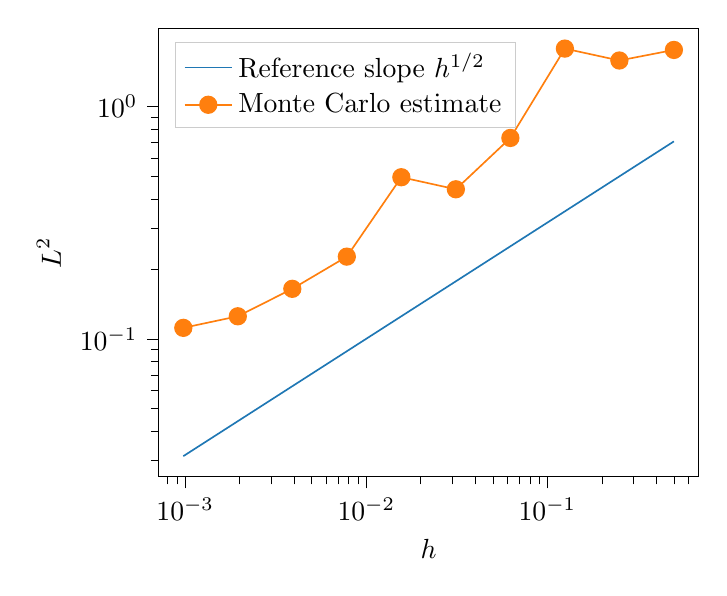
\begin{tikzpicture}

\definecolor{color0}{rgb}{0.12156862745098,0.466666666666667,0.705882352941177}
\definecolor{color1}{rgb}{1,0.498039215686275,0.0549019607843137}

\begin{axis}[
legend cell align={left},
legend style={at={(0.03,0.97)}, anchor=north west, draw=white!80.0!black},
log basis x={10},
log basis y={10},
tick align=outside,
tick pos=left,
x grid style={white!69.01960784313725!black},
xlabel={\(\displaystyle h\)},
xmin=0.000714885593723449, xmax=0.683020128377198,
xmode=log,
xtick style={color=black},
y grid style={white!69.01960784313725!black},
ylabel={\(\displaystyle L^2\)},
ymin=0.0255360184978945, ymax=2.1701192898808,
ymode=log,
ytick style={color=black}
]
\addplot [semithick, color0]
table {%
0.5 0.707106781186548
0.25 0.5
0.125 0.353553390593274
0.0625 0.25
0.03125 0.176776695296637
0.015625 0.125
0.0078125 0.0883883476483184
0.00390625 0.0625
0.001953125 0.0441941738241592
0.0009765625 0.03125
};
\addlegendentry{Reference slope $h^{1/2}$}
\addplot [semithick, color1, mark=*, mark size=3, mark options={solid}]
table {%
0.5 1.75014260105983
0.25 1.576146457538
0.125 1.77331860252908
0.0625 0.731547448485629
0.03125 0.439935234524465
0.015625 0.495737707003121
0.0078125 0.225692254063595
0.00390625 0.16405491074084
0.001953125 0.124975924343975
0.0009765625 0.11144154388575
};
\addlegendentry{Monte Carlo estimate}
\end{axis}

\end{tikzpicture}
	\caption{Log-log plot of the Monte Carlo estimate of the strong error for different $h_i, \, i = 1, \ldots, 10$,
	with the added reference slope $h^{1/2}$. \label{fig:strong_error}}
\end{figure}

\section{Assignment 4}
\subsection{Problem}
With Monte Carlo, $M = 1000$, estimate the weak error,
with the test function $\phi = \mathrm{Id}$,
for all $h_i, i = 1, \ldots, 10$.
Plot $h$ versus the weak error in a log-log plot with the added reference slope $h$.
\subsection{Theory and implementation}
For a suitable test function $\phi: \mathbb R \to \mathbb R$,
the \emph{weak error} is given by
\def\weakerror{\left|\mathbb E[\phi(X(T))] - \mathbb E[\phi(X_h(T))]\right|}
$$ \weakerror $$
The family $X_h$ \emph{converges weakly} to $X$ if
$$ \weakerror \xrightarrow[h \to 0]{} 0 \quad \forall \text{test functions} \; \phi $$
and at the \emph{rate} $\gamma$
if $\exists C, H$ such that $\forall h < H: \; \weakerror \le Ch^\gamma$.
It can be approximated with a Monte Carlo simulation by
$$ \weakerror \approx \left|\mathbb E[\phi(X(T))] - \frac1M \sum_{m=1}^M \phi(X_h(T))^{(m)}\right| $$
for a large $M \in \mathbb N$,
where we know $\mathbb E[\Id(X_h(T))] = \exp(\mu)$.

The Monte Carlo simulation of the error is sensitive to the value of $M$.
It behaves additively; the total error is
$$ \frac1{\sqrt M} + h^\gamma $$
\subsection{Results and discussion}
The plot of the weak error is found in figure~\ref{fig:weak_error}.
We see that for the larger values of $h$ the Monte Carlo estimates
of the weak error mostly seem to follow the reference slope $h$,
while for the smaller values of $h$ the weak error is larger.
This can be explained by the Monte Carlo error dominating the total error
when $h$ is small -
we see that increasing $M$ consistently decreases the total error.
Repeating the argument in section~\ref{sec:strong_error}, then,
$X_h$ would converge weakly to $X$ with the rate $1$.
This is in line with the general heuristic that
the weak rate of convergence should be twice that of the strong one.

\begin{figure}
	\centering
	%% Creator: Matplotlib, PGF backend
%%
%% To include the figure in your LaTeX document, write
%%   \input{<filename>.pgf}
%%
%% Make sure the required packages are loaded in your preamble
%%   \usepackage{pgf}
%%
%% Figures using additional raster images can only be included by \input if
%% they are in the same directory as the main LaTeX file. For loading figures
%% from other directories you can use the `import` package
%%   \usepackage{import}
%% and then include the figures with
%%   \import{<path to file>}{<filename>.pgf}
%%
%% Matplotlib used the following preamble
%%   \usepackage{fontspec}
%%   \setmainfont{DejaVuSerif.ttf}[Path=/home/axel/.local/lib/python3.6/site-packages/matplotlib/mpl-data/fonts/ttf/]
%%   \setsansfont{DejaVuSans.ttf}[Path=/home/axel/.local/lib/python3.6/site-packages/matplotlib/mpl-data/fonts/ttf/]
%%   \setmonofont{DejaVuSansMono.ttf}[Path=/home/axel/.local/lib/python3.6/site-packages/matplotlib/mpl-data/fonts/ttf/]
%%
\begingroup%
\makeatletter%
\begin{pgfpicture}%
\pgfpathrectangle{\pgfpointorigin}{\pgfqpoint{6.400000in}{4.800000in}}%
\pgfusepath{use as bounding box, clip}%
\begin{pgfscope}%
\pgfsetbuttcap%
\pgfsetmiterjoin%
\definecolor{currentfill}{rgb}{1.000000,1.000000,1.000000}%
\pgfsetfillcolor{currentfill}%
\pgfsetlinewidth{0.000000pt}%
\definecolor{currentstroke}{rgb}{1.000000,1.000000,1.000000}%
\pgfsetstrokecolor{currentstroke}%
\pgfsetdash{}{0pt}%
\pgfpathmoveto{\pgfqpoint{0.000000in}{0.000000in}}%
\pgfpathlineto{\pgfqpoint{6.400000in}{0.000000in}}%
\pgfpathlineto{\pgfqpoint{6.400000in}{4.800000in}}%
\pgfpathlineto{\pgfqpoint{0.000000in}{4.800000in}}%
\pgfpathclose%
\pgfusepath{fill}%
\end{pgfscope}%
\begin{pgfscope}%
\pgfsetbuttcap%
\pgfsetmiterjoin%
\definecolor{currentfill}{rgb}{1.000000,1.000000,1.000000}%
\pgfsetfillcolor{currentfill}%
\pgfsetlinewidth{0.000000pt}%
\definecolor{currentstroke}{rgb}{0.000000,0.000000,0.000000}%
\pgfsetstrokecolor{currentstroke}%
\pgfsetstrokeopacity{0.000000}%
\pgfsetdash{}{0pt}%
\pgfpathmoveto{\pgfqpoint{0.800000in}{0.528000in}}%
\pgfpathlineto{\pgfqpoint{5.760000in}{0.528000in}}%
\pgfpathlineto{\pgfqpoint{5.760000in}{4.224000in}}%
\pgfpathlineto{\pgfqpoint{0.800000in}{4.224000in}}%
\pgfpathclose%
\pgfusepath{fill}%
\end{pgfscope}%
\begin{pgfscope}%
\pgfsetbuttcap%
\pgfsetroundjoin%
\definecolor{currentfill}{rgb}{0.000000,0.000000,0.000000}%
\pgfsetfillcolor{currentfill}%
\pgfsetlinewidth{0.803000pt}%
\definecolor{currentstroke}{rgb}{0.000000,0.000000,0.000000}%
\pgfsetstrokecolor{currentstroke}%
\pgfsetdash{}{0pt}%
\pgfsys@defobject{currentmarker}{\pgfqpoint{0.000000in}{-0.048611in}}{\pgfqpoint{0.000000in}{0.000000in}}{%
\pgfpathmoveto{\pgfqpoint{0.000000in}{0.000000in}}%
\pgfpathlineto{\pgfqpoint{0.000000in}{-0.048611in}}%
\pgfusepath{stroke,fill}%
}%
\begin{pgfscope}%
\pgfsys@transformshift{1.042597in}{0.528000in}%
\pgfsys@useobject{currentmarker}{}%
\end{pgfscope}%
\end{pgfscope}%
\begin{pgfscope}%
\definecolor{textcolor}{rgb}{0.000000,0.000000,0.000000}%
\pgfsetstrokecolor{textcolor}%
\pgfsetfillcolor{textcolor}%
\pgftext[x=1.042597in,y=0.430778in,,top]{\color{textcolor}\sffamily\fontsize{10.000000}{12.000000}\selectfont \(\displaystyle {10^{-3}}\)}%
\end{pgfscope}%
\begin{pgfscope}%
\pgfsetbuttcap%
\pgfsetroundjoin%
\definecolor{currentfill}{rgb}{0.000000,0.000000,0.000000}%
\pgfsetfillcolor{currentfill}%
\pgfsetlinewidth{0.803000pt}%
\definecolor{currentstroke}{rgb}{0.000000,0.000000,0.000000}%
\pgfsetstrokecolor{currentstroke}%
\pgfsetdash{}{0pt}%
\pgfsys@defobject{currentmarker}{\pgfqpoint{0.000000in}{-0.048611in}}{\pgfqpoint{0.000000in}{0.000000in}}{%
\pgfpathmoveto{\pgfqpoint{0.000000in}{0.000000in}}%
\pgfpathlineto{\pgfqpoint{0.000000in}{-0.048611in}}%
\pgfusepath{stroke,fill}%
}%
\begin{pgfscope}%
\pgfsys@transformshift{2.706916in}{0.528000in}%
\pgfsys@useobject{currentmarker}{}%
\end{pgfscope}%
\end{pgfscope}%
\begin{pgfscope}%
\definecolor{textcolor}{rgb}{0.000000,0.000000,0.000000}%
\pgfsetstrokecolor{textcolor}%
\pgfsetfillcolor{textcolor}%
\pgftext[x=2.706916in,y=0.430778in,,top]{\color{textcolor}\sffamily\fontsize{10.000000}{12.000000}\selectfont \(\displaystyle {10^{-2}}\)}%
\end{pgfscope}%
\begin{pgfscope}%
\pgfsetbuttcap%
\pgfsetroundjoin%
\definecolor{currentfill}{rgb}{0.000000,0.000000,0.000000}%
\pgfsetfillcolor{currentfill}%
\pgfsetlinewidth{0.803000pt}%
\definecolor{currentstroke}{rgb}{0.000000,0.000000,0.000000}%
\pgfsetstrokecolor{currentstroke}%
\pgfsetdash{}{0pt}%
\pgfsys@defobject{currentmarker}{\pgfqpoint{0.000000in}{-0.048611in}}{\pgfqpoint{0.000000in}{0.000000in}}{%
\pgfpathmoveto{\pgfqpoint{0.000000in}{0.000000in}}%
\pgfpathlineto{\pgfqpoint{0.000000in}{-0.048611in}}%
\pgfusepath{stroke,fill}%
}%
\begin{pgfscope}%
\pgfsys@transformshift{4.371236in}{0.528000in}%
\pgfsys@useobject{currentmarker}{}%
\end{pgfscope}%
\end{pgfscope}%
\begin{pgfscope}%
\definecolor{textcolor}{rgb}{0.000000,0.000000,0.000000}%
\pgfsetstrokecolor{textcolor}%
\pgfsetfillcolor{textcolor}%
\pgftext[x=4.371236in,y=0.430778in,,top]{\color{textcolor}\sffamily\fontsize{10.000000}{12.000000}\selectfont \(\displaystyle {10^{-1}}\)}%
\end{pgfscope}%
\begin{pgfscope}%
\pgfsetbuttcap%
\pgfsetroundjoin%
\definecolor{currentfill}{rgb}{0.000000,0.000000,0.000000}%
\pgfsetfillcolor{currentfill}%
\pgfsetlinewidth{0.602250pt}%
\definecolor{currentstroke}{rgb}{0.000000,0.000000,0.000000}%
\pgfsetstrokecolor{currentstroke}%
\pgfsetdash{}{0pt}%
\pgfsys@defobject{currentmarker}{\pgfqpoint{0.000000in}{-0.027778in}}{\pgfqpoint{0.000000in}{0.000000in}}{%
\pgfpathmoveto{\pgfqpoint{0.000000in}{0.000000in}}%
\pgfpathlineto{\pgfqpoint{0.000000in}{-0.027778in}}%
\pgfusepath{stroke,fill}%
}%
\begin{pgfscope}%
\pgfsys@transformshift{0.881308in}{0.528000in}%
\pgfsys@useobject{currentmarker}{}%
\end{pgfscope}%
\end{pgfscope}%
\begin{pgfscope}%
\pgfsetbuttcap%
\pgfsetroundjoin%
\definecolor{currentfill}{rgb}{0.000000,0.000000,0.000000}%
\pgfsetfillcolor{currentfill}%
\pgfsetlinewidth{0.602250pt}%
\definecolor{currentstroke}{rgb}{0.000000,0.000000,0.000000}%
\pgfsetstrokecolor{currentstroke}%
\pgfsetdash{}{0pt}%
\pgfsys@defobject{currentmarker}{\pgfqpoint{0.000000in}{-0.027778in}}{\pgfqpoint{0.000000in}{0.000000in}}{%
\pgfpathmoveto{\pgfqpoint{0.000000in}{0.000000in}}%
\pgfpathlineto{\pgfqpoint{0.000000in}{-0.027778in}}%
\pgfusepath{stroke,fill}%
}%
\begin{pgfscope}%
\pgfsys@transformshift{0.966442in}{0.528000in}%
\pgfsys@useobject{currentmarker}{}%
\end{pgfscope}%
\end{pgfscope}%
\begin{pgfscope}%
\pgfsetbuttcap%
\pgfsetroundjoin%
\definecolor{currentfill}{rgb}{0.000000,0.000000,0.000000}%
\pgfsetfillcolor{currentfill}%
\pgfsetlinewidth{0.602250pt}%
\definecolor{currentstroke}{rgb}{0.000000,0.000000,0.000000}%
\pgfsetstrokecolor{currentstroke}%
\pgfsetdash{}{0pt}%
\pgfsys@defobject{currentmarker}{\pgfqpoint{0.000000in}{-0.027778in}}{\pgfqpoint{0.000000in}{0.000000in}}{%
\pgfpathmoveto{\pgfqpoint{0.000000in}{0.000000in}}%
\pgfpathlineto{\pgfqpoint{0.000000in}{-0.027778in}}%
\pgfusepath{stroke,fill}%
}%
\begin{pgfscope}%
\pgfsys@transformshift{1.543607in}{0.528000in}%
\pgfsys@useobject{currentmarker}{}%
\end{pgfscope}%
\end{pgfscope}%
\begin{pgfscope}%
\pgfsetbuttcap%
\pgfsetroundjoin%
\definecolor{currentfill}{rgb}{0.000000,0.000000,0.000000}%
\pgfsetfillcolor{currentfill}%
\pgfsetlinewidth{0.602250pt}%
\definecolor{currentstroke}{rgb}{0.000000,0.000000,0.000000}%
\pgfsetstrokecolor{currentstroke}%
\pgfsetdash{}{0pt}%
\pgfsys@defobject{currentmarker}{\pgfqpoint{0.000000in}{-0.027778in}}{\pgfqpoint{0.000000in}{0.000000in}}{%
\pgfpathmoveto{\pgfqpoint{0.000000in}{0.000000in}}%
\pgfpathlineto{\pgfqpoint{0.000000in}{-0.027778in}}%
\pgfusepath{stroke,fill}%
}%
\begin{pgfscope}%
\pgfsys@transformshift{1.836679in}{0.528000in}%
\pgfsys@useobject{currentmarker}{}%
\end{pgfscope}%
\end{pgfscope}%
\begin{pgfscope}%
\pgfsetbuttcap%
\pgfsetroundjoin%
\definecolor{currentfill}{rgb}{0.000000,0.000000,0.000000}%
\pgfsetfillcolor{currentfill}%
\pgfsetlinewidth{0.602250pt}%
\definecolor{currentstroke}{rgb}{0.000000,0.000000,0.000000}%
\pgfsetstrokecolor{currentstroke}%
\pgfsetdash{}{0pt}%
\pgfsys@defobject{currentmarker}{\pgfqpoint{0.000000in}{-0.027778in}}{\pgfqpoint{0.000000in}{0.000000in}}{%
\pgfpathmoveto{\pgfqpoint{0.000000in}{0.000000in}}%
\pgfpathlineto{\pgfqpoint{0.000000in}{-0.027778in}}%
\pgfusepath{stroke,fill}%
}%
\begin{pgfscope}%
\pgfsys@transformshift{2.044617in}{0.528000in}%
\pgfsys@useobject{currentmarker}{}%
\end{pgfscope}%
\end{pgfscope}%
\begin{pgfscope}%
\pgfsetbuttcap%
\pgfsetroundjoin%
\definecolor{currentfill}{rgb}{0.000000,0.000000,0.000000}%
\pgfsetfillcolor{currentfill}%
\pgfsetlinewidth{0.602250pt}%
\definecolor{currentstroke}{rgb}{0.000000,0.000000,0.000000}%
\pgfsetstrokecolor{currentstroke}%
\pgfsetdash{}{0pt}%
\pgfsys@defobject{currentmarker}{\pgfqpoint{0.000000in}{-0.027778in}}{\pgfqpoint{0.000000in}{0.000000in}}{%
\pgfpathmoveto{\pgfqpoint{0.000000in}{0.000000in}}%
\pgfpathlineto{\pgfqpoint{0.000000in}{-0.027778in}}%
\pgfusepath{stroke,fill}%
}%
\begin{pgfscope}%
\pgfsys@transformshift{2.205906in}{0.528000in}%
\pgfsys@useobject{currentmarker}{}%
\end{pgfscope}%
\end{pgfscope}%
\begin{pgfscope}%
\pgfsetbuttcap%
\pgfsetroundjoin%
\definecolor{currentfill}{rgb}{0.000000,0.000000,0.000000}%
\pgfsetfillcolor{currentfill}%
\pgfsetlinewidth{0.602250pt}%
\definecolor{currentstroke}{rgb}{0.000000,0.000000,0.000000}%
\pgfsetstrokecolor{currentstroke}%
\pgfsetdash{}{0pt}%
\pgfsys@defobject{currentmarker}{\pgfqpoint{0.000000in}{-0.027778in}}{\pgfqpoint{0.000000in}{0.000000in}}{%
\pgfpathmoveto{\pgfqpoint{0.000000in}{0.000000in}}%
\pgfpathlineto{\pgfqpoint{0.000000in}{-0.027778in}}%
\pgfusepath{stroke,fill}%
}%
\begin{pgfscope}%
\pgfsys@transformshift{2.337689in}{0.528000in}%
\pgfsys@useobject{currentmarker}{}%
\end{pgfscope}%
\end{pgfscope}%
\begin{pgfscope}%
\pgfsetbuttcap%
\pgfsetroundjoin%
\definecolor{currentfill}{rgb}{0.000000,0.000000,0.000000}%
\pgfsetfillcolor{currentfill}%
\pgfsetlinewidth{0.602250pt}%
\definecolor{currentstroke}{rgb}{0.000000,0.000000,0.000000}%
\pgfsetstrokecolor{currentstroke}%
\pgfsetdash{}{0pt}%
\pgfsys@defobject{currentmarker}{\pgfqpoint{0.000000in}{-0.027778in}}{\pgfqpoint{0.000000in}{0.000000in}}{%
\pgfpathmoveto{\pgfqpoint{0.000000in}{0.000000in}}%
\pgfpathlineto{\pgfqpoint{0.000000in}{-0.027778in}}%
\pgfusepath{stroke,fill}%
}%
\begin{pgfscope}%
\pgfsys@transformshift{2.449110in}{0.528000in}%
\pgfsys@useobject{currentmarker}{}%
\end{pgfscope}%
\end{pgfscope}%
\begin{pgfscope}%
\pgfsetbuttcap%
\pgfsetroundjoin%
\definecolor{currentfill}{rgb}{0.000000,0.000000,0.000000}%
\pgfsetfillcolor{currentfill}%
\pgfsetlinewidth{0.602250pt}%
\definecolor{currentstroke}{rgb}{0.000000,0.000000,0.000000}%
\pgfsetstrokecolor{currentstroke}%
\pgfsetdash{}{0pt}%
\pgfsys@defobject{currentmarker}{\pgfqpoint{0.000000in}{-0.027778in}}{\pgfqpoint{0.000000in}{0.000000in}}{%
\pgfpathmoveto{\pgfqpoint{0.000000in}{0.000000in}}%
\pgfpathlineto{\pgfqpoint{0.000000in}{-0.027778in}}%
\pgfusepath{stroke,fill}%
}%
\begin{pgfscope}%
\pgfsys@transformshift{2.545627in}{0.528000in}%
\pgfsys@useobject{currentmarker}{}%
\end{pgfscope}%
\end{pgfscope}%
\begin{pgfscope}%
\pgfsetbuttcap%
\pgfsetroundjoin%
\definecolor{currentfill}{rgb}{0.000000,0.000000,0.000000}%
\pgfsetfillcolor{currentfill}%
\pgfsetlinewidth{0.602250pt}%
\definecolor{currentstroke}{rgb}{0.000000,0.000000,0.000000}%
\pgfsetstrokecolor{currentstroke}%
\pgfsetdash{}{0pt}%
\pgfsys@defobject{currentmarker}{\pgfqpoint{0.000000in}{-0.027778in}}{\pgfqpoint{0.000000in}{0.000000in}}{%
\pgfpathmoveto{\pgfqpoint{0.000000in}{0.000000in}}%
\pgfpathlineto{\pgfqpoint{0.000000in}{-0.027778in}}%
\pgfusepath{stroke,fill}%
}%
\begin{pgfscope}%
\pgfsys@transformshift{2.630761in}{0.528000in}%
\pgfsys@useobject{currentmarker}{}%
\end{pgfscope}%
\end{pgfscope}%
\begin{pgfscope}%
\pgfsetbuttcap%
\pgfsetroundjoin%
\definecolor{currentfill}{rgb}{0.000000,0.000000,0.000000}%
\pgfsetfillcolor{currentfill}%
\pgfsetlinewidth{0.602250pt}%
\definecolor{currentstroke}{rgb}{0.000000,0.000000,0.000000}%
\pgfsetstrokecolor{currentstroke}%
\pgfsetdash{}{0pt}%
\pgfsys@defobject{currentmarker}{\pgfqpoint{0.000000in}{-0.027778in}}{\pgfqpoint{0.000000in}{0.000000in}}{%
\pgfpathmoveto{\pgfqpoint{0.000000in}{0.000000in}}%
\pgfpathlineto{\pgfqpoint{0.000000in}{-0.027778in}}%
\pgfusepath{stroke,fill}%
}%
\begin{pgfscope}%
\pgfsys@transformshift{3.207927in}{0.528000in}%
\pgfsys@useobject{currentmarker}{}%
\end{pgfscope}%
\end{pgfscope}%
\begin{pgfscope}%
\pgfsetbuttcap%
\pgfsetroundjoin%
\definecolor{currentfill}{rgb}{0.000000,0.000000,0.000000}%
\pgfsetfillcolor{currentfill}%
\pgfsetlinewidth{0.602250pt}%
\definecolor{currentstroke}{rgb}{0.000000,0.000000,0.000000}%
\pgfsetstrokecolor{currentstroke}%
\pgfsetdash{}{0pt}%
\pgfsys@defobject{currentmarker}{\pgfqpoint{0.000000in}{-0.027778in}}{\pgfqpoint{0.000000in}{0.000000in}}{%
\pgfpathmoveto{\pgfqpoint{0.000000in}{0.000000in}}%
\pgfpathlineto{\pgfqpoint{0.000000in}{-0.027778in}}%
\pgfusepath{stroke,fill}%
}%
\begin{pgfscope}%
\pgfsys@transformshift{3.500999in}{0.528000in}%
\pgfsys@useobject{currentmarker}{}%
\end{pgfscope}%
\end{pgfscope}%
\begin{pgfscope}%
\pgfsetbuttcap%
\pgfsetroundjoin%
\definecolor{currentfill}{rgb}{0.000000,0.000000,0.000000}%
\pgfsetfillcolor{currentfill}%
\pgfsetlinewidth{0.602250pt}%
\definecolor{currentstroke}{rgb}{0.000000,0.000000,0.000000}%
\pgfsetstrokecolor{currentstroke}%
\pgfsetdash{}{0pt}%
\pgfsys@defobject{currentmarker}{\pgfqpoint{0.000000in}{-0.027778in}}{\pgfqpoint{0.000000in}{0.000000in}}{%
\pgfpathmoveto{\pgfqpoint{0.000000in}{0.000000in}}%
\pgfpathlineto{\pgfqpoint{0.000000in}{-0.027778in}}%
\pgfusepath{stroke,fill}%
}%
\begin{pgfscope}%
\pgfsys@transformshift{3.708937in}{0.528000in}%
\pgfsys@useobject{currentmarker}{}%
\end{pgfscope}%
\end{pgfscope}%
\begin{pgfscope}%
\pgfsetbuttcap%
\pgfsetroundjoin%
\definecolor{currentfill}{rgb}{0.000000,0.000000,0.000000}%
\pgfsetfillcolor{currentfill}%
\pgfsetlinewidth{0.602250pt}%
\definecolor{currentstroke}{rgb}{0.000000,0.000000,0.000000}%
\pgfsetstrokecolor{currentstroke}%
\pgfsetdash{}{0pt}%
\pgfsys@defobject{currentmarker}{\pgfqpoint{0.000000in}{-0.027778in}}{\pgfqpoint{0.000000in}{0.000000in}}{%
\pgfpathmoveto{\pgfqpoint{0.000000in}{0.000000in}}%
\pgfpathlineto{\pgfqpoint{0.000000in}{-0.027778in}}%
\pgfusepath{stroke,fill}%
}%
\begin{pgfscope}%
\pgfsys@transformshift{3.870226in}{0.528000in}%
\pgfsys@useobject{currentmarker}{}%
\end{pgfscope}%
\end{pgfscope}%
\begin{pgfscope}%
\pgfsetbuttcap%
\pgfsetroundjoin%
\definecolor{currentfill}{rgb}{0.000000,0.000000,0.000000}%
\pgfsetfillcolor{currentfill}%
\pgfsetlinewidth{0.602250pt}%
\definecolor{currentstroke}{rgb}{0.000000,0.000000,0.000000}%
\pgfsetstrokecolor{currentstroke}%
\pgfsetdash{}{0pt}%
\pgfsys@defobject{currentmarker}{\pgfqpoint{0.000000in}{-0.027778in}}{\pgfqpoint{0.000000in}{0.000000in}}{%
\pgfpathmoveto{\pgfqpoint{0.000000in}{0.000000in}}%
\pgfpathlineto{\pgfqpoint{0.000000in}{-0.027778in}}%
\pgfusepath{stroke,fill}%
}%
\begin{pgfscope}%
\pgfsys@transformshift{4.002009in}{0.528000in}%
\pgfsys@useobject{currentmarker}{}%
\end{pgfscope}%
\end{pgfscope}%
\begin{pgfscope}%
\pgfsetbuttcap%
\pgfsetroundjoin%
\definecolor{currentfill}{rgb}{0.000000,0.000000,0.000000}%
\pgfsetfillcolor{currentfill}%
\pgfsetlinewidth{0.602250pt}%
\definecolor{currentstroke}{rgb}{0.000000,0.000000,0.000000}%
\pgfsetstrokecolor{currentstroke}%
\pgfsetdash{}{0pt}%
\pgfsys@defobject{currentmarker}{\pgfqpoint{0.000000in}{-0.027778in}}{\pgfqpoint{0.000000in}{0.000000in}}{%
\pgfpathmoveto{\pgfqpoint{0.000000in}{0.000000in}}%
\pgfpathlineto{\pgfqpoint{0.000000in}{-0.027778in}}%
\pgfusepath{stroke,fill}%
}%
\begin{pgfscope}%
\pgfsys@transformshift{4.113430in}{0.528000in}%
\pgfsys@useobject{currentmarker}{}%
\end{pgfscope}%
\end{pgfscope}%
\begin{pgfscope}%
\pgfsetbuttcap%
\pgfsetroundjoin%
\definecolor{currentfill}{rgb}{0.000000,0.000000,0.000000}%
\pgfsetfillcolor{currentfill}%
\pgfsetlinewidth{0.602250pt}%
\definecolor{currentstroke}{rgb}{0.000000,0.000000,0.000000}%
\pgfsetstrokecolor{currentstroke}%
\pgfsetdash{}{0pt}%
\pgfsys@defobject{currentmarker}{\pgfqpoint{0.000000in}{-0.027778in}}{\pgfqpoint{0.000000in}{0.000000in}}{%
\pgfpathmoveto{\pgfqpoint{0.000000in}{0.000000in}}%
\pgfpathlineto{\pgfqpoint{0.000000in}{-0.027778in}}%
\pgfusepath{stroke,fill}%
}%
\begin{pgfscope}%
\pgfsys@transformshift{4.209947in}{0.528000in}%
\pgfsys@useobject{currentmarker}{}%
\end{pgfscope}%
\end{pgfscope}%
\begin{pgfscope}%
\pgfsetbuttcap%
\pgfsetroundjoin%
\definecolor{currentfill}{rgb}{0.000000,0.000000,0.000000}%
\pgfsetfillcolor{currentfill}%
\pgfsetlinewidth{0.602250pt}%
\definecolor{currentstroke}{rgb}{0.000000,0.000000,0.000000}%
\pgfsetstrokecolor{currentstroke}%
\pgfsetdash{}{0pt}%
\pgfsys@defobject{currentmarker}{\pgfqpoint{0.000000in}{-0.027778in}}{\pgfqpoint{0.000000in}{0.000000in}}{%
\pgfpathmoveto{\pgfqpoint{0.000000in}{0.000000in}}%
\pgfpathlineto{\pgfqpoint{0.000000in}{-0.027778in}}%
\pgfusepath{stroke,fill}%
}%
\begin{pgfscope}%
\pgfsys@transformshift{4.295081in}{0.528000in}%
\pgfsys@useobject{currentmarker}{}%
\end{pgfscope}%
\end{pgfscope}%
\begin{pgfscope}%
\pgfsetbuttcap%
\pgfsetroundjoin%
\definecolor{currentfill}{rgb}{0.000000,0.000000,0.000000}%
\pgfsetfillcolor{currentfill}%
\pgfsetlinewidth{0.602250pt}%
\definecolor{currentstroke}{rgb}{0.000000,0.000000,0.000000}%
\pgfsetstrokecolor{currentstroke}%
\pgfsetdash{}{0pt}%
\pgfsys@defobject{currentmarker}{\pgfqpoint{0.000000in}{-0.027778in}}{\pgfqpoint{0.000000in}{0.000000in}}{%
\pgfpathmoveto{\pgfqpoint{0.000000in}{0.000000in}}%
\pgfpathlineto{\pgfqpoint{0.000000in}{-0.027778in}}%
\pgfusepath{stroke,fill}%
}%
\begin{pgfscope}%
\pgfsys@transformshift{4.872246in}{0.528000in}%
\pgfsys@useobject{currentmarker}{}%
\end{pgfscope}%
\end{pgfscope}%
\begin{pgfscope}%
\pgfsetbuttcap%
\pgfsetroundjoin%
\definecolor{currentfill}{rgb}{0.000000,0.000000,0.000000}%
\pgfsetfillcolor{currentfill}%
\pgfsetlinewidth{0.602250pt}%
\definecolor{currentstroke}{rgb}{0.000000,0.000000,0.000000}%
\pgfsetstrokecolor{currentstroke}%
\pgfsetdash{}{0pt}%
\pgfsys@defobject{currentmarker}{\pgfqpoint{0.000000in}{-0.027778in}}{\pgfqpoint{0.000000in}{0.000000in}}{%
\pgfpathmoveto{\pgfqpoint{0.000000in}{0.000000in}}%
\pgfpathlineto{\pgfqpoint{0.000000in}{-0.027778in}}%
\pgfusepath{stroke,fill}%
}%
\begin{pgfscope}%
\pgfsys@transformshift{5.165318in}{0.528000in}%
\pgfsys@useobject{currentmarker}{}%
\end{pgfscope}%
\end{pgfscope}%
\begin{pgfscope}%
\pgfsetbuttcap%
\pgfsetroundjoin%
\definecolor{currentfill}{rgb}{0.000000,0.000000,0.000000}%
\pgfsetfillcolor{currentfill}%
\pgfsetlinewidth{0.602250pt}%
\definecolor{currentstroke}{rgb}{0.000000,0.000000,0.000000}%
\pgfsetstrokecolor{currentstroke}%
\pgfsetdash{}{0pt}%
\pgfsys@defobject{currentmarker}{\pgfqpoint{0.000000in}{-0.027778in}}{\pgfqpoint{0.000000in}{0.000000in}}{%
\pgfpathmoveto{\pgfqpoint{0.000000in}{0.000000in}}%
\pgfpathlineto{\pgfqpoint{0.000000in}{-0.027778in}}%
\pgfusepath{stroke,fill}%
}%
\begin{pgfscope}%
\pgfsys@transformshift{5.373256in}{0.528000in}%
\pgfsys@useobject{currentmarker}{}%
\end{pgfscope}%
\end{pgfscope}%
\begin{pgfscope}%
\pgfsetbuttcap%
\pgfsetroundjoin%
\definecolor{currentfill}{rgb}{0.000000,0.000000,0.000000}%
\pgfsetfillcolor{currentfill}%
\pgfsetlinewidth{0.602250pt}%
\definecolor{currentstroke}{rgb}{0.000000,0.000000,0.000000}%
\pgfsetstrokecolor{currentstroke}%
\pgfsetdash{}{0pt}%
\pgfsys@defobject{currentmarker}{\pgfqpoint{0.000000in}{-0.027778in}}{\pgfqpoint{0.000000in}{0.000000in}}{%
\pgfpathmoveto{\pgfqpoint{0.000000in}{0.000000in}}%
\pgfpathlineto{\pgfqpoint{0.000000in}{-0.027778in}}%
\pgfusepath{stroke,fill}%
}%
\begin{pgfscope}%
\pgfsys@transformshift{5.534545in}{0.528000in}%
\pgfsys@useobject{currentmarker}{}%
\end{pgfscope}%
\end{pgfscope}%
\begin{pgfscope}%
\pgfsetbuttcap%
\pgfsetroundjoin%
\definecolor{currentfill}{rgb}{0.000000,0.000000,0.000000}%
\pgfsetfillcolor{currentfill}%
\pgfsetlinewidth{0.602250pt}%
\definecolor{currentstroke}{rgb}{0.000000,0.000000,0.000000}%
\pgfsetstrokecolor{currentstroke}%
\pgfsetdash{}{0pt}%
\pgfsys@defobject{currentmarker}{\pgfqpoint{0.000000in}{-0.027778in}}{\pgfqpoint{0.000000in}{0.000000in}}{%
\pgfpathmoveto{\pgfqpoint{0.000000in}{0.000000in}}%
\pgfpathlineto{\pgfqpoint{0.000000in}{-0.027778in}}%
\pgfusepath{stroke,fill}%
}%
\begin{pgfscope}%
\pgfsys@transformshift{5.666328in}{0.528000in}%
\pgfsys@useobject{currentmarker}{}%
\end{pgfscope}%
\end{pgfscope}%
\begin{pgfscope}%
\pgfsetbuttcap%
\pgfsetroundjoin%
\definecolor{currentfill}{rgb}{0.000000,0.000000,0.000000}%
\pgfsetfillcolor{currentfill}%
\pgfsetlinewidth{0.803000pt}%
\definecolor{currentstroke}{rgb}{0.000000,0.000000,0.000000}%
\pgfsetstrokecolor{currentstroke}%
\pgfsetdash{}{0pt}%
\pgfsys@defobject{currentmarker}{\pgfqpoint{-0.048611in}{0.000000in}}{\pgfqpoint{0.000000in}{0.000000in}}{%
\pgfpathmoveto{\pgfqpoint{0.000000in}{0.000000in}}%
\pgfpathlineto{\pgfqpoint{-0.048611in}{0.000000in}}%
\pgfusepath{stroke,fill}%
}%
\begin{pgfscope}%
\pgfsys@transformshift{0.800000in}{0.708774in}%
\pgfsys@useobject{currentmarker}{}%
\end{pgfscope}%
\end{pgfscope}%
\begin{pgfscope}%
\definecolor{textcolor}{rgb}{0.000000,0.000000,0.000000}%
\pgfsetstrokecolor{textcolor}%
\pgfsetfillcolor{textcolor}%
\pgftext[x=0.414775in,y=0.656012in,left,base]{\color{textcolor}\sffamily\fontsize{10.000000}{12.000000}\selectfont \(\displaystyle {10^{-3}}\)}%
\end{pgfscope}%
\begin{pgfscope}%
\pgfsetbuttcap%
\pgfsetroundjoin%
\definecolor{currentfill}{rgb}{0.000000,0.000000,0.000000}%
\pgfsetfillcolor{currentfill}%
\pgfsetlinewidth{0.803000pt}%
\definecolor{currentstroke}{rgb}{0.000000,0.000000,0.000000}%
\pgfsetstrokecolor{currentstroke}%
\pgfsetdash{}{0pt}%
\pgfsys@defobject{currentmarker}{\pgfqpoint{-0.048611in}{0.000000in}}{\pgfqpoint{0.000000in}{0.000000in}}{%
\pgfpathmoveto{\pgfqpoint{0.000000in}{0.000000in}}%
\pgfpathlineto{\pgfqpoint{-0.048611in}{0.000000in}}%
\pgfusepath{stroke,fill}%
}%
\begin{pgfscope}%
\pgfsys@transformshift{0.800000in}{1.948960in}%
\pgfsys@useobject{currentmarker}{}%
\end{pgfscope}%
\end{pgfscope}%
\begin{pgfscope}%
\definecolor{textcolor}{rgb}{0.000000,0.000000,0.000000}%
\pgfsetstrokecolor{textcolor}%
\pgfsetfillcolor{textcolor}%
\pgftext[x=0.414775in,y=1.896199in,left,base]{\color{textcolor}\sffamily\fontsize{10.000000}{12.000000}\selectfont \(\displaystyle {10^{-2}}\)}%
\end{pgfscope}%
\begin{pgfscope}%
\pgfsetbuttcap%
\pgfsetroundjoin%
\definecolor{currentfill}{rgb}{0.000000,0.000000,0.000000}%
\pgfsetfillcolor{currentfill}%
\pgfsetlinewidth{0.803000pt}%
\definecolor{currentstroke}{rgb}{0.000000,0.000000,0.000000}%
\pgfsetstrokecolor{currentstroke}%
\pgfsetdash{}{0pt}%
\pgfsys@defobject{currentmarker}{\pgfqpoint{-0.048611in}{0.000000in}}{\pgfqpoint{0.000000in}{0.000000in}}{%
\pgfpathmoveto{\pgfqpoint{0.000000in}{0.000000in}}%
\pgfpathlineto{\pgfqpoint{-0.048611in}{0.000000in}}%
\pgfusepath{stroke,fill}%
}%
\begin{pgfscope}%
\pgfsys@transformshift{0.800000in}{3.189147in}%
\pgfsys@useobject{currentmarker}{}%
\end{pgfscope}%
\end{pgfscope}%
\begin{pgfscope}%
\definecolor{textcolor}{rgb}{0.000000,0.000000,0.000000}%
\pgfsetstrokecolor{textcolor}%
\pgfsetfillcolor{textcolor}%
\pgftext[x=0.414775in,y=3.136385in,left,base]{\color{textcolor}\sffamily\fontsize{10.000000}{12.000000}\selectfont \(\displaystyle {10^{-1}}\)}%
\end{pgfscope}%
\begin{pgfscope}%
\pgfsetbuttcap%
\pgfsetroundjoin%
\definecolor{currentfill}{rgb}{0.000000,0.000000,0.000000}%
\pgfsetfillcolor{currentfill}%
\pgfsetlinewidth{0.602250pt}%
\definecolor{currentstroke}{rgb}{0.000000,0.000000,0.000000}%
\pgfsetstrokecolor{currentstroke}%
\pgfsetdash{}{0pt}%
\pgfsys@defobject{currentmarker}{\pgfqpoint{-0.027778in}{0.000000in}}{\pgfqpoint{0.000000in}{0.000000in}}{%
\pgfpathmoveto{\pgfqpoint{0.000000in}{0.000000in}}%
\pgfpathlineto{\pgfqpoint{-0.027778in}{0.000000in}}%
\pgfusepath{stroke,fill}%
}%
\begin{pgfscope}%
\pgfsys@transformshift{0.800000in}{0.588587in}%
\pgfsys@useobject{currentmarker}{}%
\end{pgfscope}%
\end{pgfscope}%
\begin{pgfscope}%
\pgfsetbuttcap%
\pgfsetroundjoin%
\definecolor{currentfill}{rgb}{0.000000,0.000000,0.000000}%
\pgfsetfillcolor{currentfill}%
\pgfsetlinewidth{0.602250pt}%
\definecolor{currentstroke}{rgb}{0.000000,0.000000,0.000000}%
\pgfsetstrokecolor{currentstroke}%
\pgfsetdash{}{0pt}%
\pgfsys@defobject{currentmarker}{\pgfqpoint{-0.027778in}{0.000000in}}{\pgfqpoint{0.000000in}{0.000000in}}{%
\pgfpathmoveto{\pgfqpoint{0.000000in}{0.000000in}}%
\pgfpathlineto{\pgfqpoint{-0.027778in}{0.000000in}}%
\pgfusepath{stroke,fill}%
}%
\begin{pgfscope}%
\pgfsys@transformshift{0.800000in}{0.652026in}%
\pgfsys@useobject{currentmarker}{}%
\end{pgfscope}%
\end{pgfscope}%
\begin{pgfscope}%
\pgfsetbuttcap%
\pgfsetroundjoin%
\definecolor{currentfill}{rgb}{0.000000,0.000000,0.000000}%
\pgfsetfillcolor{currentfill}%
\pgfsetlinewidth{0.602250pt}%
\definecolor{currentstroke}{rgb}{0.000000,0.000000,0.000000}%
\pgfsetstrokecolor{currentstroke}%
\pgfsetdash{}{0pt}%
\pgfsys@defobject{currentmarker}{\pgfqpoint{-0.027778in}{0.000000in}}{\pgfqpoint{0.000000in}{0.000000in}}{%
\pgfpathmoveto{\pgfqpoint{0.000000in}{0.000000in}}%
\pgfpathlineto{\pgfqpoint{-0.027778in}{0.000000in}}%
\pgfusepath{stroke,fill}%
}%
\begin{pgfscope}%
\pgfsys@transformshift{0.800000in}{1.082107in}%
\pgfsys@useobject{currentmarker}{}%
\end{pgfscope}%
\end{pgfscope}%
\begin{pgfscope}%
\pgfsetbuttcap%
\pgfsetroundjoin%
\definecolor{currentfill}{rgb}{0.000000,0.000000,0.000000}%
\pgfsetfillcolor{currentfill}%
\pgfsetlinewidth{0.602250pt}%
\definecolor{currentstroke}{rgb}{0.000000,0.000000,0.000000}%
\pgfsetstrokecolor{currentstroke}%
\pgfsetdash{}{0pt}%
\pgfsys@defobject{currentmarker}{\pgfqpoint{-0.027778in}{0.000000in}}{\pgfqpoint{0.000000in}{0.000000in}}{%
\pgfpathmoveto{\pgfqpoint{0.000000in}{0.000000in}}%
\pgfpathlineto{\pgfqpoint{-0.027778in}{0.000000in}}%
\pgfusepath{stroke,fill}%
}%
\begin{pgfscope}%
\pgfsys@transformshift{0.800000in}{1.300493in}%
\pgfsys@useobject{currentmarker}{}%
\end{pgfscope}%
\end{pgfscope}%
\begin{pgfscope}%
\pgfsetbuttcap%
\pgfsetroundjoin%
\definecolor{currentfill}{rgb}{0.000000,0.000000,0.000000}%
\pgfsetfillcolor{currentfill}%
\pgfsetlinewidth{0.602250pt}%
\definecolor{currentstroke}{rgb}{0.000000,0.000000,0.000000}%
\pgfsetstrokecolor{currentstroke}%
\pgfsetdash{}{0pt}%
\pgfsys@defobject{currentmarker}{\pgfqpoint{-0.027778in}{0.000000in}}{\pgfqpoint{0.000000in}{0.000000in}}{%
\pgfpathmoveto{\pgfqpoint{0.000000in}{0.000000in}}%
\pgfpathlineto{\pgfqpoint{-0.027778in}{0.000000in}}%
\pgfusepath{stroke,fill}%
}%
\begin{pgfscope}%
\pgfsys@transformshift{0.800000in}{1.455441in}%
\pgfsys@useobject{currentmarker}{}%
\end{pgfscope}%
\end{pgfscope}%
\begin{pgfscope}%
\pgfsetbuttcap%
\pgfsetroundjoin%
\definecolor{currentfill}{rgb}{0.000000,0.000000,0.000000}%
\pgfsetfillcolor{currentfill}%
\pgfsetlinewidth{0.602250pt}%
\definecolor{currentstroke}{rgb}{0.000000,0.000000,0.000000}%
\pgfsetstrokecolor{currentstroke}%
\pgfsetdash{}{0pt}%
\pgfsys@defobject{currentmarker}{\pgfqpoint{-0.027778in}{0.000000in}}{\pgfqpoint{0.000000in}{0.000000in}}{%
\pgfpathmoveto{\pgfqpoint{0.000000in}{0.000000in}}%
\pgfpathlineto{\pgfqpoint{-0.027778in}{0.000000in}}%
\pgfusepath{stroke,fill}%
}%
\begin{pgfscope}%
\pgfsys@transformshift{0.800000in}{1.575627in}%
\pgfsys@useobject{currentmarker}{}%
\end{pgfscope}%
\end{pgfscope}%
\begin{pgfscope}%
\pgfsetbuttcap%
\pgfsetroundjoin%
\definecolor{currentfill}{rgb}{0.000000,0.000000,0.000000}%
\pgfsetfillcolor{currentfill}%
\pgfsetlinewidth{0.602250pt}%
\definecolor{currentstroke}{rgb}{0.000000,0.000000,0.000000}%
\pgfsetstrokecolor{currentstroke}%
\pgfsetdash{}{0pt}%
\pgfsys@defobject{currentmarker}{\pgfqpoint{-0.027778in}{0.000000in}}{\pgfqpoint{0.000000in}{0.000000in}}{%
\pgfpathmoveto{\pgfqpoint{0.000000in}{0.000000in}}%
\pgfpathlineto{\pgfqpoint{-0.027778in}{0.000000in}}%
\pgfusepath{stroke,fill}%
}%
\begin{pgfscope}%
\pgfsys@transformshift{0.800000in}{1.673827in}%
\pgfsys@useobject{currentmarker}{}%
\end{pgfscope}%
\end{pgfscope}%
\begin{pgfscope}%
\pgfsetbuttcap%
\pgfsetroundjoin%
\definecolor{currentfill}{rgb}{0.000000,0.000000,0.000000}%
\pgfsetfillcolor{currentfill}%
\pgfsetlinewidth{0.602250pt}%
\definecolor{currentstroke}{rgb}{0.000000,0.000000,0.000000}%
\pgfsetstrokecolor{currentstroke}%
\pgfsetdash{}{0pt}%
\pgfsys@defobject{currentmarker}{\pgfqpoint{-0.027778in}{0.000000in}}{\pgfqpoint{0.000000in}{0.000000in}}{%
\pgfpathmoveto{\pgfqpoint{0.000000in}{0.000000in}}%
\pgfpathlineto{\pgfqpoint{-0.027778in}{0.000000in}}%
\pgfusepath{stroke,fill}%
}%
\begin{pgfscope}%
\pgfsys@transformshift{0.800000in}{1.756853in}%
\pgfsys@useobject{currentmarker}{}%
\end{pgfscope}%
\end{pgfscope}%
\begin{pgfscope}%
\pgfsetbuttcap%
\pgfsetroundjoin%
\definecolor{currentfill}{rgb}{0.000000,0.000000,0.000000}%
\pgfsetfillcolor{currentfill}%
\pgfsetlinewidth{0.602250pt}%
\definecolor{currentstroke}{rgb}{0.000000,0.000000,0.000000}%
\pgfsetstrokecolor{currentstroke}%
\pgfsetdash{}{0pt}%
\pgfsys@defobject{currentmarker}{\pgfqpoint{-0.027778in}{0.000000in}}{\pgfqpoint{0.000000in}{0.000000in}}{%
\pgfpathmoveto{\pgfqpoint{0.000000in}{0.000000in}}%
\pgfpathlineto{\pgfqpoint{-0.027778in}{0.000000in}}%
\pgfusepath{stroke,fill}%
}%
\begin{pgfscope}%
\pgfsys@transformshift{0.800000in}{1.828774in}%
\pgfsys@useobject{currentmarker}{}%
\end{pgfscope}%
\end{pgfscope}%
\begin{pgfscope}%
\pgfsetbuttcap%
\pgfsetroundjoin%
\definecolor{currentfill}{rgb}{0.000000,0.000000,0.000000}%
\pgfsetfillcolor{currentfill}%
\pgfsetlinewidth{0.602250pt}%
\definecolor{currentstroke}{rgb}{0.000000,0.000000,0.000000}%
\pgfsetstrokecolor{currentstroke}%
\pgfsetdash{}{0pt}%
\pgfsys@defobject{currentmarker}{\pgfqpoint{-0.027778in}{0.000000in}}{\pgfqpoint{0.000000in}{0.000000in}}{%
\pgfpathmoveto{\pgfqpoint{0.000000in}{0.000000in}}%
\pgfpathlineto{\pgfqpoint{-0.027778in}{0.000000in}}%
\pgfusepath{stroke,fill}%
}%
\begin{pgfscope}%
\pgfsys@transformshift{0.800000in}{1.892213in}%
\pgfsys@useobject{currentmarker}{}%
\end{pgfscope}%
\end{pgfscope}%
\begin{pgfscope}%
\pgfsetbuttcap%
\pgfsetroundjoin%
\definecolor{currentfill}{rgb}{0.000000,0.000000,0.000000}%
\pgfsetfillcolor{currentfill}%
\pgfsetlinewidth{0.602250pt}%
\definecolor{currentstroke}{rgb}{0.000000,0.000000,0.000000}%
\pgfsetstrokecolor{currentstroke}%
\pgfsetdash{}{0pt}%
\pgfsys@defobject{currentmarker}{\pgfqpoint{-0.027778in}{0.000000in}}{\pgfqpoint{0.000000in}{0.000000in}}{%
\pgfpathmoveto{\pgfqpoint{0.000000in}{0.000000in}}%
\pgfpathlineto{\pgfqpoint{-0.027778in}{0.000000in}}%
\pgfusepath{stroke,fill}%
}%
\begin{pgfscope}%
\pgfsys@transformshift{0.800000in}{2.322294in}%
\pgfsys@useobject{currentmarker}{}%
\end{pgfscope}%
\end{pgfscope}%
\begin{pgfscope}%
\pgfsetbuttcap%
\pgfsetroundjoin%
\definecolor{currentfill}{rgb}{0.000000,0.000000,0.000000}%
\pgfsetfillcolor{currentfill}%
\pgfsetlinewidth{0.602250pt}%
\definecolor{currentstroke}{rgb}{0.000000,0.000000,0.000000}%
\pgfsetstrokecolor{currentstroke}%
\pgfsetdash{}{0pt}%
\pgfsys@defobject{currentmarker}{\pgfqpoint{-0.027778in}{0.000000in}}{\pgfqpoint{0.000000in}{0.000000in}}{%
\pgfpathmoveto{\pgfqpoint{0.000000in}{0.000000in}}%
\pgfpathlineto{\pgfqpoint{-0.027778in}{0.000000in}}%
\pgfusepath{stroke,fill}%
}%
\begin{pgfscope}%
\pgfsys@transformshift{0.800000in}{2.540680in}%
\pgfsys@useobject{currentmarker}{}%
\end{pgfscope}%
\end{pgfscope}%
\begin{pgfscope}%
\pgfsetbuttcap%
\pgfsetroundjoin%
\definecolor{currentfill}{rgb}{0.000000,0.000000,0.000000}%
\pgfsetfillcolor{currentfill}%
\pgfsetlinewidth{0.602250pt}%
\definecolor{currentstroke}{rgb}{0.000000,0.000000,0.000000}%
\pgfsetstrokecolor{currentstroke}%
\pgfsetdash{}{0pt}%
\pgfsys@defobject{currentmarker}{\pgfqpoint{-0.027778in}{0.000000in}}{\pgfqpoint{0.000000in}{0.000000in}}{%
\pgfpathmoveto{\pgfqpoint{0.000000in}{0.000000in}}%
\pgfpathlineto{\pgfqpoint{-0.027778in}{0.000000in}}%
\pgfusepath{stroke,fill}%
}%
\begin{pgfscope}%
\pgfsys@transformshift{0.800000in}{2.695627in}%
\pgfsys@useobject{currentmarker}{}%
\end{pgfscope}%
\end{pgfscope}%
\begin{pgfscope}%
\pgfsetbuttcap%
\pgfsetroundjoin%
\definecolor{currentfill}{rgb}{0.000000,0.000000,0.000000}%
\pgfsetfillcolor{currentfill}%
\pgfsetlinewidth{0.602250pt}%
\definecolor{currentstroke}{rgb}{0.000000,0.000000,0.000000}%
\pgfsetstrokecolor{currentstroke}%
\pgfsetdash{}{0pt}%
\pgfsys@defobject{currentmarker}{\pgfqpoint{-0.027778in}{0.000000in}}{\pgfqpoint{0.000000in}{0.000000in}}{%
\pgfpathmoveto{\pgfqpoint{0.000000in}{0.000000in}}%
\pgfpathlineto{\pgfqpoint{-0.027778in}{0.000000in}}%
\pgfusepath{stroke,fill}%
}%
\begin{pgfscope}%
\pgfsys@transformshift{0.800000in}{2.815814in}%
\pgfsys@useobject{currentmarker}{}%
\end{pgfscope}%
\end{pgfscope}%
\begin{pgfscope}%
\pgfsetbuttcap%
\pgfsetroundjoin%
\definecolor{currentfill}{rgb}{0.000000,0.000000,0.000000}%
\pgfsetfillcolor{currentfill}%
\pgfsetlinewidth{0.602250pt}%
\definecolor{currentstroke}{rgb}{0.000000,0.000000,0.000000}%
\pgfsetstrokecolor{currentstroke}%
\pgfsetdash{}{0pt}%
\pgfsys@defobject{currentmarker}{\pgfqpoint{-0.027778in}{0.000000in}}{\pgfqpoint{0.000000in}{0.000000in}}{%
\pgfpathmoveto{\pgfqpoint{0.000000in}{0.000000in}}%
\pgfpathlineto{\pgfqpoint{-0.027778in}{0.000000in}}%
\pgfusepath{stroke,fill}%
}%
\begin{pgfscope}%
\pgfsys@transformshift{0.800000in}{2.914013in}%
\pgfsys@useobject{currentmarker}{}%
\end{pgfscope}%
\end{pgfscope}%
\begin{pgfscope}%
\pgfsetbuttcap%
\pgfsetroundjoin%
\definecolor{currentfill}{rgb}{0.000000,0.000000,0.000000}%
\pgfsetfillcolor{currentfill}%
\pgfsetlinewidth{0.602250pt}%
\definecolor{currentstroke}{rgb}{0.000000,0.000000,0.000000}%
\pgfsetstrokecolor{currentstroke}%
\pgfsetdash{}{0pt}%
\pgfsys@defobject{currentmarker}{\pgfqpoint{-0.027778in}{0.000000in}}{\pgfqpoint{0.000000in}{0.000000in}}{%
\pgfpathmoveto{\pgfqpoint{0.000000in}{0.000000in}}%
\pgfpathlineto{\pgfqpoint{-0.027778in}{0.000000in}}%
\pgfusepath{stroke,fill}%
}%
\begin{pgfscope}%
\pgfsys@transformshift{0.800000in}{2.997040in}%
\pgfsys@useobject{currentmarker}{}%
\end{pgfscope}%
\end{pgfscope}%
\begin{pgfscope}%
\pgfsetbuttcap%
\pgfsetroundjoin%
\definecolor{currentfill}{rgb}{0.000000,0.000000,0.000000}%
\pgfsetfillcolor{currentfill}%
\pgfsetlinewidth{0.602250pt}%
\definecolor{currentstroke}{rgb}{0.000000,0.000000,0.000000}%
\pgfsetstrokecolor{currentstroke}%
\pgfsetdash{}{0pt}%
\pgfsys@defobject{currentmarker}{\pgfqpoint{-0.027778in}{0.000000in}}{\pgfqpoint{0.000000in}{0.000000in}}{%
\pgfpathmoveto{\pgfqpoint{0.000000in}{0.000000in}}%
\pgfpathlineto{\pgfqpoint{-0.027778in}{0.000000in}}%
\pgfusepath{stroke,fill}%
}%
\begin{pgfscope}%
\pgfsys@transformshift{0.800000in}{3.068960in}%
\pgfsys@useobject{currentmarker}{}%
\end{pgfscope}%
\end{pgfscope}%
\begin{pgfscope}%
\pgfsetbuttcap%
\pgfsetroundjoin%
\definecolor{currentfill}{rgb}{0.000000,0.000000,0.000000}%
\pgfsetfillcolor{currentfill}%
\pgfsetlinewidth{0.602250pt}%
\definecolor{currentstroke}{rgb}{0.000000,0.000000,0.000000}%
\pgfsetstrokecolor{currentstroke}%
\pgfsetdash{}{0pt}%
\pgfsys@defobject{currentmarker}{\pgfqpoint{-0.027778in}{0.000000in}}{\pgfqpoint{0.000000in}{0.000000in}}{%
\pgfpathmoveto{\pgfqpoint{0.000000in}{0.000000in}}%
\pgfpathlineto{\pgfqpoint{-0.027778in}{0.000000in}}%
\pgfusepath{stroke,fill}%
}%
\begin{pgfscope}%
\pgfsys@transformshift{0.800000in}{3.132399in}%
\pgfsys@useobject{currentmarker}{}%
\end{pgfscope}%
\end{pgfscope}%
\begin{pgfscope}%
\pgfsetbuttcap%
\pgfsetroundjoin%
\definecolor{currentfill}{rgb}{0.000000,0.000000,0.000000}%
\pgfsetfillcolor{currentfill}%
\pgfsetlinewidth{0.602250pt}%
\definecolor{currentstroke}{rgb}{0.000000,0.000000,0.000000}%
\pgfsetstrokecolor{currentstroke}%
\pgfsetdash{}{0pt}%
\pgfsys@defobject{currentmarker}{\pgfqpoint{-0.027778in}{0.000000in}}{\pgfqpoint{0.000000in}{0.000000in}}{%
\pgfpathmoveto{\pgfqpoint{0.000000in}{0.000000in}}%
\pgfpathlineto{\pgfqpoint{-0.027778in}{0.000000in}}%
\pgfusepath{stroke,fill}%
}%
\begin{pgfscope}%
\pgfsys@transformshift{0.800000in}{3.562480in}%
\pgfsys@useobject{currentmarker}{}%
\end{pgfscope}%
\end{pgfscope}%
\begin{pgfscope}%
\pgfsetbuttcap%
\pgfsetroundjoin%
\definecolor{currentfill}{rgb}{0.000000,0.000000,0.000000}%
\pgfsetfillcolor{currentfill}%
\pgfsetlinewidth{0.602250pt}%
\definecolor{currentstroke}{rgb}{0.000000,0.000000,0.000000}%
\pgfsetstrokecolor{currentstroke}%
\pgfsetdash{}{0pt}%
\pgfsys@defobject{currentmarker}{\pgfqpoint{-0.027778in}{0.000000in}}{\pgfqpoint{0.000000in}{0.000000in}}{%
\pgfpathmoveto{\pgfqpoint{0.000000in}{0.000000in}}%
\pgfpathlineto{\pgfqpoint{-0.027778in}{0.000000in}}%
\pgfusepath{stroke,fill}%
}%
\begin{pgfscope}%
\pgfsys@transformshift{0.800000in}{3.780866in}%
\pgfsys@useobject{currentmarker}{}%
\end{pgfscope}%
\end{pgfscope}%
\begin{pgfscope}%
\pgfsetbuttcap%
\pgfsetroundjoin%
\definecolor{currentfill}{rgb}{0.000000,0.000000,0.000000}%
\pgfsetfillcolor{currentfill}%
\pgfsetlinewidth{0.602250pt}%
\definecolor{currentstroke}{rgb}{0.000000,0.000000,0.000000}%
\pgfsetstrokecolor{currentstroke}%
\pgfsetdash{}{0pt}%
\pgfsys@defobject{currentmarker}{\pgfqpoint{-0.027778in}{0.000000in}}{\pgfqpoint{0.000000in}{0.000000in}}{%
\pgfpathmoveto{\pgfqpoint{0.000000in}{0.000000in}}%
\pgfpathlineto{\pgfqpoint{-0.027778in}{0.000000in}}%
\pgfusepath{stroke,fill}%
}%
\begin{pgfscope}%
\pgfsys@transformshift{0.800000in}{3.935814in}%
\pgfsys@useobject{currentmarker}{}%
\end{pgfscope}%
\end{pgfscope}%
\begin{pgfscope}%
\pgfsetbuttcap%
\pgfsetroundjoin%
\definecolor{currentfill}{rgb}{0.000000,0.000000,0.000000}%
\pgfsetfillcolor{currentfill}%
\pgfsetlinewidth{0.602250pt}%
\definecolor{currentstroke}{rgb}{0.000000,0.000000,0.000000}%
\pgfsetstrokecolor{currentstroke}%
\pgfsetdash{}{0pt}%
\pgfsys@defobject{currentmarker}{\pgfqpoint{-0.027778in}{0.000000in}}{\pgfqpoint{0.000000in}{0.000000in}}{%
\pgfpathmoveto{\pgfqpoint{0.000000in}{0.000000in}}%
\pgfpathlineto{\pgfqpoint{-0.027778in}{0.000000in}}%
\pgfusepath{stroke,fill}%
}%
\begin{pgfscope}%
\pgfsys@transformshift{0.800000in}{4.056000in}%
\pgfsys@useobject{currentmarker}{}%
\end{pgfscope}%
\end{pgfscope}%
\begin{pgfscope}%
\pgfsetbuttcap%
\pgfsetroundjoin%
\definecolor{currentfill}{rgb}{0.000000,0.000000,0.000000}%
\pgfsetfillcolor{currentfill}%
\pgfsetlinewidth{0.602250pt}%
\definecolor{currentstroke}{rgb}{0.000000,0.000000,0.000000}%
\pgfsetstrokecolor{currentstroke}%
\pgfsetdash{}{0pt}%
\pgfsys@defobject{currentmarker}{\pgfqpoint{-0.027778in}{0.000000in}}{\pgfqpoint{0.000000in}{0.000000in}}{%
\pgfpathmoveto{\pgfqpoint{0.000000in}{0.000000in}}%
\pgfpathlineto{\pgfqpoint{-0.027778in}{0.000000in}}%
\pgfusepath{stroke,fill}%
}%
\begin{pgfscope}%
\pgfsys@transformshift{0.800000in}{4.154200in}%
\pgfsys@useobject{currentmarker}{}%
\end{pgfscope}%
\end{pgfscope}%
\begin{pgfscope}%
\pgfpathrectangle{\pgfqpoint{0.800000in}{0.528000in}}{\pgfqpoint{4.960000in}{3.696000in}}%
\pgfusepath{clip}%
\pgfsetrectcap%
\pgfsetroundjoin%
\pgfsetlinewidth{1.505625pt}%
\definecolor{currentstroke}{rgb}{0.121569,0.466667,0.705882}%
\pgfsetstrokecolor{currentstroke}%
\pgfsetdash{}{0pt}%
\pgfpathmoveto{\pgfqpoint{5.534545in}{4.056000in}}%
\pgfpathlineto{\pgfqpoint{5.033535in}{3.682667in}}%
\pgfpathlineto{\pgfqpoint{4.532525in}{3.309333in}}%
\pgfpathlineto{\pgfqpoint{4.031515in}{2.936000in}}%
\pgfpathlineto{\pgfqpoint{3.530505in}{2.562667in}}%
\pgfpathlineto{\pgfqpoint{3.029495in}{2.189333in}}%
\pgfpathlineto{\pgfqpoint{2.528485in}{1.816000in}}%
\pgfpathlineto{\pgfqpoint{2.027475in}{1.442667in}}%
\pgfpathlineto{\pgfqpoint{1.526465in}{1.069333in}}%
\pgfpathlineto{\pgfqpoint{1.025455in}{0.696000in}}%
\pgfusepath{stroke}%
\end{pgfscope}%
\begin{pgfscope}%
\pgfpathrectangle{\pgfqpoint{0.800000in}{0.528000in}}{\pgfqpoint{4.960000in}{3.696000in}}%
\pgfusepath{clip}%
\pgfsetrectcap%
\pgfsetroundjoin%
\pgfsetlinewidth{1.505625pt}%
\definecolor{currentstroke}{rgb}{1.000000,0.498039,0.054902}%
\pgfsetstrokecolor{currentstroke}%
\pgfsetdash{}{0pt}%
\pgfpathmoveto{\pgfqpoint{5.534545in}{4.008458in}}%
\pgfpathlineto{\pgfqpoint{5.033535in}{3.937624in}}%
\pgfpathlineto{\pgfqpoint{4.532525in}{2.548070in}}%
\pgfpathlineto{\pgfqpoint{4.031515in}{2.660307in}}%
\pgfpathlineto{\pgfqpoint{3.530505in}{2.356606in}}%
\pgfpathlineto{\pgfqpoint{3.029495in}{3.479209in}}%
\pgfpathlineto{\pgfqpoint{2.528485in}{2.763962in}}%
\pgfpathlineto{\pgfqpoint{2.027475in}{2.575075in}}%
\pgfpathlineto{\pgfqpoint{1.526465in}{2.737336in}}%
\pgfpathlineto{\pgfqpoint{1.025455in}{3.259308in}}%
\pgfusepath{stroke}%
\end{pgfscope}%
\begin{pgfscope}%
\pgfsetrectcap%
\pgfsetmiterjoin%
\pgfsetlinewidth{0.803000pt}%
\definecolor{currentstroke}{rgb}{0.000000,0.000000,0.000000}%
\pgfsetstrokecolor{currentstroke}%
\pgfsetdash{}{0pt}%
\pgfpathmoveto{\pgfqpoint{0.800000in}{0.528000in}}%
\pgfpathlineto{\pgfqpoint{0.800000in}{4.224000in}}%
\pgfusepath{stroke}%
\end{pgfscope}%
\begin{pgfscope}%
\pgfsetrectcap%
\pgfsetmiterjoin%
\pgfsetlinewidth{0.803000pt}%
\definecolor{currentstroke}{rgb}{0.000000,0.000000,0.000000}%
\pgfsetstrokecolor{currentstroke}%
\pgfsetdash{}{0pt}%
\pgfpathmoveto{\pgfqpoint{5.760000in}{0.528000in}}%
\pgfpathlineto{\pgfqpoint{5.760000in}{4.224000in}}%
\pgfusepath{stroke}%
\end{pgfscope}%
\begin{pgfscope}%
\pgfsetrectcap%
\pgfsetmiterjoin%
\pgfsetlinewidth{0.803000pt}%
\definecolor{currentstroke}{rgb}{0.000000,0.000000,0.000000}%
\pgfsetstrokecolor{currentstroke}%
\pgfsetdash{}{0pt}%
\pgfpathmoveto{\pgfqpoint{0.800000in}{0.528000in}}%
\pgfpathlineto{\pgfqpoint{5.760000in}{0.528000in}}%
\pgfusepath{stroke}%
\end{pgfscope}%
\begin{pgfscope}%
\pgfsetrectcap%
\pgfsetmiterjoin%
\pgfsetlinewidth{0.803000pt}%
\definecolor{currentstroke}{rgb}{0.000000,0.000000,0.000000}%
\pgfsetstrokecolor{currentstroke}%
\pgfsetdash{}{0pt}%
\pgfpathmoveto{\pgfqpoint{0.800000in}{4.224000in}}%
\pgfpathlineto{\pgfqpoint{5.760000in}{4.224000in}}%
\pgfusepath{stroke}%
\end{pgfscope}%
\begin{pgfscope}%
\definecolor{textcolor}{rgb}{0.000000,0.000000,0.000000}%
\pgfsetstrokecolor{textcolor}%
\pgfsetfillcolor{textcolor}%
\pgftext[x=3.280000in,y=4.307333in,,base]{\color{textcolor}\sffamily\fontsize{12.000000}{14.400000}\selectfont Weak error of |E[X(1)] - E[X\_h(1)]|}%
\end{pgfscope}%
\begin{pgfscope}%
\pgfsetbuttcap%
\pgfsetmiterjoin%
\definecolor{currentfill}{rgb}{1.000000,1.000000,1.000000}%
\pgfsetfillcolor{currentfill}%
\pgfsetfillopacity{0.800000}%
\pgfsetlinewidth{1.003750pt}%
\definecolor{currentstroke}{rgb}{0.800000,0.800000,0.800000}%
\pgfsetstrokecolor{currentstroke}%
\pgfsetstrokeopacity{0.800000}%
\pgfsetdash{}{0pt}%
\pgfpathmoveto{\pgfqpoint{0.897222in}{3.909032in}}%
\pgfpathlineto{\pgfqpoint{2.586919in}{3.909032in}}%
\pgfpathquadraticcurveto{\pgfqpoint{2.614697in}{3.909032in}}{\pgfqpoint{2.614697in}{3.936809in}}%
\pgfpathlineto{\pgfqpoint{2.614697in}{4.126778in}}%
\pgfpathquadraticcurveto{\pgfqpoint{2.614697in}{4.154556in}}{\pgfqpoint{2.586919in}{4.154556in}}%
\pgfpathlineto{\pgfqpoint{0.897222in}{4.154556in}}%
\pgfpathquadraticcurveto{\pgfqpoint{0.869444in}{4.154556in}}{\pgfqpoint{0.869444in}{4.126778in}}%
\pgfpathlineto{\pgfqpoint{0.869444in}{3.936809in}}%
\pgfpathquadraticcurveto{\pgfqpoint{0.869444in}{3.909032in}}{\pgfqpoint{0.897222in}{3.909032in}}%
\pgfpathclose%
\pgfusepath{stroke,fill}%
\end{pgfscope}%
\begin{pgfscope}%
\pgfsetrectcap%
\pgfsetroundjoin%
\pgfsetlinewidth{1.505625pt}%
\definecolor{currentstroke}{rgb}{0.121569,0.466667,0.705882}%
\pgfsetstrokecolor{currentstroke}%
\pgfsetdash{}{0pt}%
\pgfpathmoveto{\pgfqpoint{0.925000in}{4.042088in}}%
\pgfpathlineto{\pgfqpoint{1.202778in}{4.042088in}}%
\pgfusepath{stroke}%
\end{pgfscope}%
\begin{pgfscope}%
\definecolor{textcolor}{rgb}{0.000000,0.000000,0.000000}%
\pgfsetstrokecolor{textcolor}%
\pgfsetfillcolor{textcolor}%
\pgftext[x=1.313889in,y=3.993477in,left,base]{\color{textcolor}\sffamily\fontsize{10.000000}{12.000000}\selectfont Reference slope h}%
\end{pgfscope}%
\end{pgfpicture}%
\makeatother%
\endgroup%

	\caption{Log-log plot of the Monte Carlo estimate of the weak error for different $h_i, i = 1, \ldots, 10$,
	with the added reference slope $h$. \label{fig:weak_error}}
\end{figure}

\clearpage
\appendix % Start appendix sections

\section{Python code}
\lstinputlisting[language=Python]{lab6.py}

\end{document}
